%% ----------------------------------------------------------------
%% Thesis.tex -- MAIN FILE (the one that you compile with LaTeX)
%% ----------------------------------------------------------------

% Set up the document
\documentclass[a4paper, 11pt, oneside]{Thesis}  % Use the "Thesis" style, based on the ECS Thesis style by Steve Gunn
\graphicspath{Figures/}  % Location of the graphics files (set up for graphics to be in PDF format)


\usepackage[table,xcdraw]{xcolor}
\usepackage{fancyvrb}
% Include any extra LaTeX packages required
\usepackage[square, authoryear, comma]{natbib}  % 
%Use the "Natbib" style for the references in the Bibliography
%\usepackage[backend=biber,style=alphabetic,sorting=nyt]{biblatex}
\usepackage{verbatim}  % Needed for the "comment" environment to make LaTeX comments
\usepackage{vector}  % Allows "\bvec{}" and "\buvec{}" for "blackboard" style bold vectors in maths
\hypersetup{urlcolor=blue, colorlinks=true}  % Colours hyperlinks in blue, but this can be distracting if there are many links.

\newcommand{\bilinearroot}{Chapters/bilinear}

\newcommand{\fig}[1]{Figure~\ref{fig:#1}}
\newcommand{\pr}[1]{Problem~\ref{pr:#1}}
\newcommand{\sect}[1]{Section~\ref{sect:#1}}
\newcommand{\chapt}[1]{Chapter~\ref{chapt:#1}}
\newcommand{\tab}[1]{Table~\ref{tab:#1}}
\newcommand{\alg}[1]{Algorithm~\ref{alg:#1}}
\newcommand{\eq}[1]{(\ref{eq:#1})}
\newcommand*{\tran}{^{\mkern-1.5mu\mathsf{T}}}
\usepackage{verbatimbox}
\usepackage{todonotes}
\usepackage{gensymb}
\usepackage{enumitem}

%\usepackage{subfigure}
\usepackage{graphicx}
%\usepackage{caption}
\usepackage{subcaption}
\newcommand{\ie}{\textit{i}.\textit{e}.,}
\newcommand{\eg}{\textit{e}.\textit{g}.,}
%\newcommand{\todo}[1][]{\@latex@warning{TODO #1}\fbox{TODO\dots}}


\usepackage{tabularx,lipsum,environ,amsmath,amssymb}
\newcounter{problemcounter}
\renewcommand{\theproblemcounter}{\arabic{problemcounter}}
\makeatletter
\newcommand{\problemtitle}[1]{\gdef\@problemtitle{#1}}% Store problem title
\newcommand{\probleminput}[1]{\gdef\@probleminput{#1}}% Store problem input
\newcommand{\problemquestion}[1]{\gdef\@problemquestion{#1}}% Store problem question
\NewEnviron{problem}{
\refstepcounter{problemcounter}
\label{#1}%

   \problemtitle{}
   \probleminput{}\problemquestion{}% Default input is empty
  \BODY% Parse input
  \par\addvspace{.5\baselineskip}
  \noindent
  \begin{tabularx}{\textwidth}{@{\hspace{\parindent}} l X c}
    \multicolumn{2}{@{\hspace{\parindent}}l}{Problem~\theproblemcounter. \textit{\@problemtitle}} \\% Title
    \hline
    \textbf{Input:} & \@probleminput \\% Input
    \textbf{Task:} & \@problemquestion% Question
    \\\hline
  \end{tabularx}
  \par\addvspace{.5\baselineskip}
}

%\usepackage{amsmath,amssymb} % define this before the line numbering.
%\usepackage{placeins}
%\usepackage{color}
%\usepackage[width=122mm,left=12mm,paperwidth=146mm,height=193mm,top=12mm,paperheight=217mm]{geometry}
%\usepackage{subfigure}
%\usepackage{subcaption}
%\usepackage{xr-hyper}
%\usepackage[colorlinks=true]{hyperref}
%\usepackage{textcomp}

% Tikz-related stuff.
\usepackage{tikz}
\usetikzlibrary{arrows.meta}
\usetikzlibrary{backgrounds}
\usetikzlibrary{calc}
\usetikzlibrary{decorations.markings}
\usetikzlibrary{decorations.text}
\usetikzlibrary{fit}
\usetikzlibrary{positioning}
\usetikzlibrary{shapes.geometric}
\usetikzlibrary{3d}

% PGF-plots-related stuff.
\usepackage{pgfplots}
\usepgfplotslibrary{groupplots}
\pgfplotsset{compat=newest}

% \usepgfplotslibrary{external}
% \tikzexternalize

\usepackage{nomencl}
\makenomenclature
\renewcommand{\nomname}{List of Abbreviations}

\newcommand{\Sp}{{\mathcal S}^{+}}
\newcommand{\Sgen}{{\mathcal S}}
\newcommand{\Sm}{{\mathcal S}^{-}}
\newcommand{\spr}[2]{{\langle{}#1,#2\rangle}}
\newcommand{\prp}{p^{+}}
\newcommand{\prm}{p^{-}}
\newcommand{\Hp}{H^{+}}
\newcommand{\Hm}{H^{-}}
\newcommand{\hp}{h^{+}}
\newcommand{\hm}{h^{-}}

%%%%%%%%GRADREV HEADER

  
    \usepackage{subfig}
    \usepackage{algorithm}
    \usepackage{algorithmic}
    \usepackage{amsmath}
    \usepackage{amssymb}
    \usepackage{amsfonts}
    \usepackage{dsfont}
    \usepackage{xspace}
    \usepackage{xr}
    \usepackage{multirow}
    \usepackage{multicol}
    \usepackage{siunitx}
    \usepackage{afterpage}
    \usepackage{bbm}
    \usepackage{enumerate}
    \usepackage{booktabs}
    \usepackage{natbib}
    \usepackage{soul}
    \usepackage{mathtools}
    %\usepackage[colorlinks=false,allbordercolors={1 1 1}]{hyperref}
    %\usepackage[hidelinks]{hyperref}
    
    % Moscow header
  %  \newcommand{\theHalgorithm}{\arabic{algorithm}}
    \newcommand{\dataset}{{\cal D}}
    \newcommand{\fracpartial}[2]{\frac{\partial #1}{\partial  #2}}
    
     
    \def\x{{\mathbf x}}
    \def\f{{\mathbf f}}
    
    \def\S{{\cal S}}
    \def\T{{\cal T}}
    
    \def\R{{\mathds R}}
    
    \def\tf{{\theta_f}}
    \def\td{{\theta_d}}
    \def\ty{{\theta_y}}
    \def\htf{{\hat\theta_f}}
    \def\htd{{\hat\theta_d}}
    \def\hty{{\hat\theta_y}}
    \newcommand{\ys}{y}
    \newcommand{\yt}{y}

    % uncertainty is separated with a "plus-minus" symbol
    \sisetup{separate-uncertainty=true}
    
    \usepackage{tikz}
    \usetikzlibrary{positioning}
    \usetikzlibrary{calc}
    
    \usepackage{pgfplots}
    \pgfplotsset{compat=newest} 
    \pgfplotsset{plot coordinates/math parser=false}
    
    % This is needed for plots.
    \newlength\figureheight
    \newlength\figurewidth
    
    
    %\newcommand{\subfig}[1]{{\em(#1)}}
    
    %\renewcommand{\topfraction}{0.85}
    %\renewcommand{\textfraction}{0.1}
    %\renewcommand{\floatpagefraction}{0.85}
    %\parskip 0pt
    
    \makeatletter
    \newcommand{\todo}[1][]{\@latex@warning{TODO #1}\fbox{TODO\dots}}
    \makeatother
    
    
    % Quebec's header
    
    
    \newcommand{\phib}{{\pmb \phi}}
    \newcommand{\uu}{{\mathbf{u}}}
    %\renewcommand{\ww}{\uu}
    
    \newcommand{\redplus}{``\red{$\boldsymbol{{+}}$}''}
    \newcommand{\greenminus}{``\green{$\boldsymbol{{\pmb{-}}}$}''}
    
    % To harmonize the transatlantic notation! 
    \renewcommand{\eqdef}{=}
    \newcommand{\Acal}{{\mathcal{A}}}
    \newcommand{\Xcal}{{\mathcal{X}}}
    \newcommand{\Ycal}{{\mathcal{Y}}}
    \newcommand{\Lcal}{{\mathcal{L}}}
    \newcommand{\Dcal}{{\mathcal{D}}}
    \newcommand{\Hcal}{{\mathcal{H}}}
    \renewcommand{\Xcal}{X}
    \renewcommand{\Ycal}{Y}
    \newcommand{\dsum}{\displaystyle\sum}
    \newcommand{\dprod}{\displaystyle\prod}
    
    
    \DeclareMathOperator*{\argmax}{\mathrm{argmax}}
    \DeclareMathOperator*{\argmin}{\mathrm{argmin}}
    
    \newcommand{\DS}{{\Dcal_\textsc{S}}}
    \newcommand{\DT}{{\Dcal_\textsc{T}}}
    \newcommand{\DSX}{{\Dcal_\textsc{S}^{_\Xcal}}}
    \newcommand{\DTX}{{\Dcal_\textsc{T}^{_\Xcal}}}
    
    \newcommand{\RDS}{R_{\DS}}
    \newcommand{\RDT}{R_{\DT}}
    \newcommand{\RS}{R_{S}}
    \newcommand{\RD}{R_{D}}
    \renewcommand{\S}{\DSX}
    \renewcommand{\T}{\DTX}
    \newcommand{\xb}{{\mathbf x}}
    \newcommand{\yb}{{\mathbf y}}



\usepackage{nomencl}
\makenomenclature
 
\renewcommand{\nomname}{List of abbreviations}

%%%%%%%%
\def\mystrut{\rule[-.3\baselineskip]{0pt}{0.5\baselineskip}}

\definecolor{inodefill}{HTML}{D9EAD3}
\definecolor{inodedraw}{HTML}{B6D7A8}
\definecolor{pnodefill}{HTML}{CFE2F3}
\definecolor{pnodedraw}{HTML}{9FC5E8}
\definecolor{onodefill}{HTML}{E6B8AF}
\definecolor{onodedraw}{HTML}{CC4125}
\definecolor{mnodefill}{HTML}{EAD1DC}
\definecolor{mnodedraw}{HTML}{D5A6BD}
\definecolor{goldfill}{HTML}{EAD7AC}
\definecolor{golddraw}{HTML}{D1AC71}
\definecolor{bluefill}{HTML}{5AB1F2}
\definecolor{bluedraw}{HTML}{0083E5}


%% ----------------------------------------------------------------
\begin{document}

\begin{titlepage}
 \begin{center}
 \phantom{a}\vspace{3.2cm}
 

\includegraphics[width=6cm]{sk.png}
  
  \large% SKOLKOVO INSTITUTE OF SCIENCE AND TECHNOLOGY
  \vspace{3.2cm}
  
  {\LARGE\bf Deep learning systems for 3D Reconstruction problems}
  \vspace{3cm}
  
  { \sl Doctoral Thesis\medskip
  
  by}\medskip
  
  Alexandr Notchenko
  \vspace{2cm}

  
  
  
 \end{center}

\end{titlepage}


\frontmatter      % Begin Roman style (i, ii, iii, iv...) page numbering

% Set up the Title Page
\title  {Deep learning systems for 3D Reconstruction problems}
\authors  {Alexandr Notchenko}
\addresses  {\groupname\\\deptname\\\univname}  % Do not change this here, instead these must be set in the "Thesis.cls" file, please look through it instead
\date       {\today}
\subject    {}
\keywords   {}

\maketitle
%% ----------------------------------------------------------------

\setstretch{1.3}  % It is better to have smaller font and larger line spacing than the other way round

% Define the page headers using the FancyHdr package and set up for one-sided printing
\fancyhead{}  % Clears all page headers and footers
\rhead{\thepage}  % Sets the right side header to show the page number
\lhead{}  % Clears the left side page header

\pagestyle{fancy}  % Finally, use the "fancy" page style to implement the FancyHdr headers

%% ----------------------------------------------------------------
% Declaration Page required for the Thesis, your institution may give you a different text to place here
%\Declaration{

%\addtocontents{toc}{\vspace{1em}}  % Add a gap in the Contents, for aesthetics

%I, AUTHOR NAME, declare that this thesis titled, `THESIS TITLE' and the work presented in it are my own. I confirm that:

%\begin{itemize}
%\item[\tiny{$\blacksquare$}] This work was done wholly or mainly while in candidature for a research degree at this University.

%\item[\tiny{$\blacksquare$}] Where any part of this thesis has previously been submitted for a degree or any other qualification at this University or any other institution, this has been clearly stated.

%\item[\tiny{$\blacksquare$}] Where I have consulted the published work of others, this is always clearly attributed.

%\item[\tiny{$\blacksquare$}] Where I have quoted from the work of others, the source is always given. With the exception of such quotations, this thesis is entirely my own work.

%\item[\tiny{$\blacksquare$}] I have acknowledged all main sources of help.

%\item[\tiny{$\blacksquare$}] Where the thesis is based on work done by myself jointly with others, I have made clear exactly what was done by others and what I have contributed myself.
%\\
%\end{itemize}


%Signed:\\
%\rule[1em]{25em}{0.5pt}  % This prints a line for the signature

%Date:\\
%\rule[1em]{25em}{0.5pt}  % This prints a line to write the date
%}
%\clearpage  % Declaration ended, now start a new page

%% ----------------------------------------------------------------
% The "Funny Quote Page"
%\pagestyle{empty}  % No headers or footers for the following pages

%\null\vfill
% Now comes the "Funny Quote", written in italics
%\textit{``You're just too good to be true \\
%Can't take my eyes off you.''}

%\begin{flushright}
%Bob Crewe, Bob Gaudio
%\end{flushright}

%\vfill\vfill\vfill\vfill\vfill\vfill\null
%\clearpage  % Funny Quote page ended, start a new page
%% ----------------------------------------------------------------

% The Abstract Page
\addtotoc{Abstract}  % Add the "Abstract" page entry to the Contents
\abstract{
\addtocontents{toc}{\vspace{1em}}  % Add a gap in the Contents, for aesthetics

This work considers two popular human recognition problems,   namely, person re-identification and face recognition. For both of these tasks, similarity estimation for pairs of images is the core problem. Generally, no examples of test identities are exposed
during the training stage, so the system should be able to learn the similarity concept from the training data and to generalize it onto unseen identities.

Training of siamese neural networks is at the center of this work. Provided with an appropriate objective function, they are able to learn a mapping from an input image space to a high-dimensional descriptor space in such a way that the semantic similarity of input images can be estimated using Euclidean distance or angular similarity between the corresponding embeddings (descriptors). Three important aspects of building siamese deep neural networks for person re-identification are considered: the architecture design, the objective function design, and deep domain adaptation techniques. Domain adaptation is additionally considered for face recognition. 

While deep learning has approached human performance in face recognition, the results for person re-identification have been relatively modest during recent time. Two improvements related to training siamese neural networks for person re-identification are suggested in this work. First of them is a loss function for siamese training, called Histogram loss. The new loss does not introduce parameters that need to be tuned and shows favorable results across a range of datasets and problems compared to recently proposed alternatives. Second, a new architecture for person re-identification is suggested. As the task of re-identification is inherently associated with non-rigid appearance description, the suggested architecture is based on the deep bilinear convolutional network (Bilinear CNN) that has been proposed recently for fine-grained classification of highly non-rigid objects. Finally, domain adaptation is addressed for both person re-identification and a special case of face recognition related to using surveillance data at the test stage. Domain adversarial training is adopted for person re-identification and shown to improve the results in the cross-domain setting. Feature-level and more recent image-level deep adaptation techniques are evaluated and viable strategies are suggested for surveillance face recognition.



}

\clearpage  % Abstract ended, start a new page
%% ----------------------------------------------------------------

{\large
 List of publications:}



\begin{itemize}
    \item 
Yaroslav Ganin, Evgeniya Ustinova, Hana Ajakan, Pascal Germain, Hugo Larochelle, Fran\c{c}ois Laviolette, Mario Marchand and Victor Lempitsky. Domain-adversarial training of neural networks. The Journal of Machine Learning Research, JMLR, 17(1), pages 2096-2030, 2016.
 \textit{Personal contribution: developing the variant of the method for similarity learning, designing and conducting the experiments for person re-identification, text writing (partially)}
           
    \item
Evgeniya Ustinova and Victor Lempitsky. Learning deep embeddings with histogram loss. Advances in Neural Information Processing Systems, NIPS, 2016.
\textit{Personal contribution: existing approaches analysis, method development, designing and conducting the experiments, text writing (partially).}
       
    \item
    Evgeniya Ustinova, Yaroslav Ganin and Victor Lempitsky,  Multi-region bilinear convolutional neural networks for person re-identification. IEEE International Conference on Advanced Video Signal-based Surveillance, AVSS, 2017.
    \textit{Personal contribution: existing approaches analysis, method development, designing and conducting the experiments, text writing (partially).}
    
\end{itemize}

\clearpage
\setstretch{1.3}  % Reset the line-spacing to 1.3 for body text (if it has changed)

% The Acknowledgements page, for thanking everyone
%\acknowledgements{
%\addtocontents{toc}{\vspace{1em}}  % Add a gap in the Contents, for aesthetics

%The acknowledgements and the people to thank go here, don't forget to include your project advisor\ldots

%}
%\clearpage  % End of the Acknowledgements
%% ----------------------------------------------------------------

\pagestyle{fancy}  %The page style headers have been "empty" all this time, now use the "fancy" headers as defined before to bring them back


%% ----------------------------------------------------------------
%\lhead{\emph{Contents}}  % Set the left side page header to "Contents"
\tableofcontents  % Write out the Table of Contents

%% ----------------------------------------------------------------
%\lhead{\emph{List of Figures}}  % Set the left side page header to "List if Figures"
%\listoffigures  % Write out the List of Figures

%% ----------------------------------------------------------------
%\lhead{\emph{List of Tables}}  % Set the left side page header to "List of Tables"
%\listoftables  % Write out the List of Tables

%% ----------------------------------------------------------------
\setstretch{1.5}  % Set the line spacing to 1.5, this makes the following tables easier to read

%\clearpage  % Start a new page
%\lhead{\emph{Abbreviations}}  % Set the left side page header to "Abbreviations"
%\listofsymbols{ll}  % Include a list of Abbreviations (a table of two columns)
%{
% \textbf{Acronym} & \textbf{W}hat (it) \textbf{S}tands \textbf{F}or \\
%\textbf{LAH} & \textbf{L}ist \textbf{A}bbreviations \textbf{H}ere \\
%
%}

%% ----------------------------------------------------------------
%\clearpage  % Start a new page
%\lhead{\emph{Physical Constants}}  % Set the left side page header to "Physical Constants"
%\listofconstants{lrcl}  % Include a list of Physical Constants (a four column table)
%{
% Constant Name & Symbol & = & Constant Value (with units) \\
%Speed of Light & $c$ & $=$ & $2.997\ 924\ 58\times10^{8}\ \mbox{ms}^{-\mbox{s}}$ (exact)\\

%}

%% ----------------------------------------------------------------
%\clearpage  %Start a new page
%\lhead{\emph{Symbols}}  % Set the left side page header to "Symbols"
%\listofnomenclature{lll}  % Include a list of Symbols (a three column table)
%{
% symbol & name & unit \\
%$a$ & distance & m \\
%$P$ & power & W (Js$^{-1}$) \\
%& & \\ % Gap to separate the Roman symbols from the Greek
%$\omega$ & angular frequency & rads$^{-1}$ \\
%}
%% ----------------------------------------------------------------
% End of the pre-able, contents and lists of things
% Begin the Dedication page

\setstretch{1.3}  % Return the line spacing back to 1.3

%\pagestyle{empty}  % Page style needs to be empty for this page
%\dedicatory{For/Dedicated to/To my\ldots}

\addtocontents{toc}{\vspace{2em}}  % Add a gap in the Contents, for aesthetics


%% ----------------------------------------------------------------
\mainmatter	  % Begin normal, numeric (1,2,3...) page numbering
\pagestyle{fancy}  % Return the page headers back to the "fancy" style

% Include the chapters of the thesis, as separate files
% Just uncomment the lines as you write the chapters




\nomenclature{CNN}{Convolutional Neural Network}
\nomenclature{PCA}{Principal Component Analysis}
\nomenclature{t-SNE}{t-distributed Stochastic Neighbor Embedding}

\nomenclature{CMC curve}{Cumulative Matching Characteristic curve}
\nomenclature{SGD}{Stochastic Gradient Descent}
\nomenclature{ReLU}{Rectified Linear Unit}
\nomenclature{CycleGAN}{Cycle-Consistent Generative Adversarial Network}
\nomenclature{DML}{Deep Metric Learning}
\nomenclature{LSSS loss}{Lifted Structured Softmax Similarity loss} 
 
 
\printnomenclature


% !TEX root = ../Thesis_main.tex
\chapter{Introduction}

%video surveillance+
%person re-id+
% originates from Multi-Target Multi-Camera Tracking 
%open world / closed world+
%face : verification/identification
%common aspects: detection , processing, recognition
%deep learning

%retrieval
%fine-grained recognition
%adaptation

%datasets (cut from the papers) + table with reid dataset?
%architectures
%definitions?
%contribution - what is done
\section{Context}
\subsection{Problem of 3D reconstruction}

\subsection{Approaches for solving 3D Reconstruction problem}

Solutions for a reconstruction problem can be grouped in two major groups: 1) Geometric approach - when problem is represented as optimisation of scene state given constrains on projections of scene state to data, 2) Machine Learning approach - inverse model is optimisation.

If $X$ - is scene data, $z$ - is the state of the scene, and $g_i(z)$ - projection function of 3D scene $z$ state to perspective $i$, then to find an optimal 3D reconstruction, one solves this minimisation problem:
\begin{equation}
z_{rec} = \min_z\sum_i|X_i-g_i(z)|_2 .
\end{equation}

This approach only solves problem for once scene and does not provide any semantic information about it, only basic geometric information. 
The second approach is more modern and better fitted for machine learning applications, because instead of optimizing state of the scene, it's optimizes a model that performs computation from input data to some semantic (intrinsic) parameters, and can be described as following optimisation procedure:
\begin{equation}
\min_\theta\sum_i|X_i-g_i(f_\theta(\pi))|_2,\ \ \pi=I_\theta(\{X_i\}_i),\ \ z=f_\theta(\pi),
\end{equation}
where $\pi$ - are scene parameters, $f_\theta(\pi)$ - is a generative model that generates 3D state $z$ and it's function is determined by tunable parameters $\theta$.

In reconstruction process information can be introduced in two possible ways: 1) input signal - data measured by some spatial sensor, 2) by adding a priori knowledge while training the Inverse model or by design choice of reconstruction algprithm. Between the two source exist a fundamental trade-off and detirmination of which is dominant can be quite difficult \cite{tatarchenko2019single}.


\subsection{Objectives and Motivations}

The goal of this work to improve methods of 3D reconstruction in holistic context using deep learning systems. For efficient applications such as robotics in human environments and mixed reality more advanced machine perception systems are needed. Human perception is a complex system with several properties not all of which are replicated in modern machine perception systems. From cognitive sciences it's known that ability to model environments is one of the most important for perception system, in area of computer vision this is known as an ability to perform \textit{3D reconstruction} of scenes and environments. To solve this problem in a general case requires application of machine learning.

In particular, the development of such holistic deep 3D reconstruction system includes several important tasks:

\begin{itemize}
􏰀    \item Capturing scenes, complete with colour and depth data of a sufficient quality,
    \item Recalling objects from large scale database of objects,
    \item Segmenting variety of most common elements from sensor data, such as household objects and architectural components,
    \item Detecting and reconstructing shape and pose of and human bodies.
\end{itemize}

Each of these sub-tasks constitutes a challenge in the context of human perception.

The presence of noise in sensor data (e.g., consumer grade depth cameras) is a serious problem for all downstream sub-tasks, low fidelity of this data causes a considerable compaunding performance drop.

\subsection{3D data representations}

We can describe a 3D object in multiple ways, and codification of it's properties has ramifications about capturing different information about objects and scenes, as well as kinds of models that can regenerate them or computational resources needed to process it.
Each representation has it's own pros and cons. We assume 3D information representation to be positive effective and usefull if it captures more relevant information with less storage requirement (compression), increases signal to noise ratio of data, captures shape and texture properties with minimum trade-off.

Here are some popular examples of 3D data representations:
\begin{enumerate}
	\item Multiple 2D projections - captures surface texture, highly redundant representation if images overlap, also vulnerable to optic illusions.
	\item Voxels - simple, most of the time can be sparse, represents rough volumetric properties vell but losses most of surface properties.
	\item Point Cloud - are sparse in a sense that they don't capture empty space, losing all surface properties besides color and estimated normals and most of volumetric properties.
	\item 2.5D (RGB-D) images are widespread because of cheap measurement devices, capture volumentric depth but succeptable to occlusion of bodies in a scene and records a lot of noise with actual signal.
\end{enumerate}



%Motivation: RGB-D scanning is here and we want to have a fine-grained understanding of the 3D captures
In the recent years, a wide variety of consumer-grade RGB-D sensors, such as the Intel Real Sense, Microsoft Kinect, depth-sensor enabled smartphones, enabled inexpensive and rapid RGB-D data acquisition. Increasing availability of large, labeled datasets (e.g.,~\cite{chang2017matterport3d,dai2017scannet})  made possible development of deep learning methods for 3D object classification and semantic segmentation. At the same time, acquired 3D data is often incomplete and noisy; while one can identify and segment the objects in the scene, reconstructing high-quality geometry of objects remains a challenging problem.  

An example of the new approach in recent work 
\cite{avetisyan2019scan2cad}, uses a large dataset of clean, labeled geometric shapes
\cite{chang2015shapenet}, for classification/segmentation associating the input point or voxel data with object labels from the dataset, along with adapting geometry to 3D data.  This approach ensures that the output geometry has high quality, and is robust with respect to noise and missing data in the input.  
At the same time, a ``flat'' classification/segmentation approach, with each object in the database corresponding to a separate label and matched to a subpart of the input data corresponding to the whole object, does not scale well as the number of classes grows and often runs into difficulties in the cases of extreme occlusion (only a relatively small part of an object is visible). 
Significant improvements can be achieved by considering object \emph{parts}, or more generally part hierarchies. 
Part-based segmentation of 3D datasets promises to offer a significant improvement both in finding the best matching shape in the dataset, recognizing objects from  highly incomplete data (e.g., from a couple of parts) from  as well as more precise geometry adaptation as well as, potentially, assembly of new shapes out of existing parts yielding a closer match to the input data. 

large collection of 3D models in database can be reduced to structured representations, 
objects with occluded sub-parts still can be recognized by parts available in the scan and the rest can be guessed with high probability, using parts, we can reconstruct new objects that are not yet present in the database of shapes.

Based on different approaches for volumetric information integration, from enhancements of  methods such as volumetric fusion \cite{curless1996volumetric}, to probabilistic  methods, and plethora of methods based on their combinations.

Compared to computer graphics models manually created by 3D professionals, 3D scans are noisy and incomplete.
Amount of noise and limited resolution of consumer-grade scanning hardware pose significant challenges for solving this important problem of scene reconstruction. 
Approaches of reconstruction based on fitting existing 3D assets into scene scans, have shown a lot of promise but still had problems with finding exact models from large database such as ShapeNet \cite{chang2015shapenet}, because of occlusion and lack of spatial context.

Learning-based approaches are very good at extracting features representative of objects and scenes as a whole, allowing to fill in occluded areas or guess parts affected by noise \cite{dai2017shape,dai2018scancomplete,song2017semantic}. These features are sufficient for scene completion, but they are not as good at recovering geometric primitives like: sharp edges, planar surfaces or borders between sub-parts, resulting in reconstruction quality much poorer than that of 3D content created by humans.

In this work, we focus on the key problem of semantic part segmentation of objects in the scenes, enabling further improvements in  dataset-based reconstruction. 
Semantic part-segmentation, can help in these situations, when sufficient number of the object parts is visible model can infer the non-visible parts essentially completing an object in sense of maximum probability conditioned on input data.

In human-made environments, a lot of objects have naturally defined semantic sub-parts, and those sub-parts can, in turn, have their sub-parts, i.e., parts form \emph{hierarchies}.  In our work, we use scene and object representation based on such part hierarchies.  We show how a part-labeled dataset of scanned 3D data suitable for machine learning applications can be constructed, and used to improve the performance of segmentation algorithms. 

Definitions of sub-parts are based on a set of primitive elements that were manufactured by one formation method or from one material.

Because of that and the fact that static scenes have other relationships between objects (fixed to each other or in direct surface contact), it's reasonable to suggest a scene description format that possesses a property of hierarchy (e.g., trees or other kinds of graphs).
Representing scenes as a discrete structures with multiple relationships between nodes. Such relationships like composability of its parts and affordances between whole objects, in turn allowing to compose a scene from separate objects.

\todo{merge these paragraphs}

In domain of human-made environments a lot of objects have sub-parts and those sub-parts can in turn have their own sub-parts. Definition of sub-part is often based on a set of primitive elements that were manufactured by one formation method or from one material. Because of that and the fact that static scenes have other relationships between objects (fixed to each other or in direct surface contact), it's reasonable to suggest a scene description format that possess a property of hierarchy (e.g. trees or other subgraphs).
A lot of researchers over the last 20 years came to the same conclusion. A lot of work on that problem was done by Mumford and Zhu in \cite{zhu2006stochastic}.

One of the papers dealt with problem of modeling Images as a hierarchy of super-pixels. \cite{russell2009associative}, or as a tree of geometric primitives (e.g. cylinders, spheres or 3D boxes) \cite{li2017grass}.

% point cloud (PC) turned in to a graph (based on proximity) point-cloud parser network reduces number of nodes and edges and enriches their feature vectors. First part of the decoder network functions similar to Feature Pyramid Network in CNNs, which performs local computations on different scales, followed by "pooling or convolutions" with reduced spatial component and increased feature components, thus leaving only small number of "keypoints" required to outline shapes of objects.



CAD constructor network translates that graph into CAD object (tree with primitives and combination rules). CAD rendered makes a mesh out of that object thus a residual between original PC and Mesh can be calculated.

Proximity Graphs - concept that allows to build a bridge between Point Clouds and Graph Processing. This area of computational geometry has a lot of theoretical results to offer for Deep Learning piplene designer.


\subsection{Definitions and examples}
\subsection{Data sources and devices}

\section{Inverse Graphics Problem formulation}

\cite{rezende2016unsupervised,eslami2016attend,kulkarni2015deep,wu20153d,izadinia2017im2cad}

Inverse graphics approach enables to solve a problem of "real-world" scene understanding through reconstruction of that scene and comparison it to measured data in some form.

Because it's a fairly new method it has some unexplored facets:
\begin{enumerate}
    \item How can we scale to hundreds and thousands of objects with different parameters.
    \item Embedded representations better than procedural generation
    \item Are there format that can have all advantages of CAD models and probabilistic properties that arise from real-world uncertainties.
\end{enumerate}

Central goals of computational perception is to get structured description of scenes from measurements such as photographic images, scans and videos.

Computer Vision as Inverse Graphics is the most rational formulations that could help us achieve this goal.

In the past, it has been hard to directly solve these problems in practice because of computational limitations.

However, it may be right time to take another look at this idea due to significant advances in deep learning for computer vision, probabilistic programming, and computer graphics.

Probabilistic programming - a tool that allows us to implement complex models while keeping ability to perform inference, extend with other probabilistic models by being general-purpose.

Re-formalizing inverse graphics in terms of probabilistic programming and deep learning allow us to solve even more complicated vision problems with off-the-shelf computational technology.

To make this approach scalable, my research can incorporate effective techniques such as: approximate Bayesian computation, differentiable programming for rendering.

Computer Graphics nowadays seems to be improving at a great pace in terms of designing solutions for hard image synthesis problems, but these solutions are usually hand-made and not flexible enough to cover all needs for general-purpose real world object generating, latest advances in generative models can help with that.


\subsection{Overcoming lack of information}

\section{Datasets}

Only recently research community started accumuulating sugnifficant amount of algined sensor data to solve large scale 3D reconstruction problems in deep learning context. In last 4 years we saw an explosion of 3D shape databases and 2D-to-3D indoor scene datasets, such as ShapeNet, 2D-3D Semantic, Scannet and Matterport3D datasets. Because accuracy and reacall properties of deep learning models scale with amount and variety of data, number of state-of-the-art models grew as well.

\section{Architectures}

PanopticFusion~\cite{narita2019panopticfusion} is a model that is able to segment large indoor scenes and separate \textit{Stuff} and \textit{Things}.


For outdoor datasets Point Cloud representation of data is more common because of large empty spaces and the way LiDAR sensor collects data. In such setting instance segmentation is nessesary first step for reconstruction~\cite{zhang2020instance}.

\subsection{Multi-view models}

Detailed comparision of multi-view 2D CNN model and 3D volumetric CNN can be found in \cite{qi2016volumetric}.

\subsection{Implicit 2D models}

Like inverse graphics network. Model takes 2D images and returns 2D images with 3D properties changed. 

\subsection{3D convolutional models}

Model generates or processes voxel image with 3D convolutional operation implemented Dense or Sparse.

Semantic information can boost the reconstruction performance because deep learning systems are able to pick up onto consistent signal \cite{jiao2018look,tatarchenko2019single,kendall2018multi}.

\subsection{2D to 3D Projection models}

Model uses camera parameters to compute 3D representation using 2D/2.5D images and projection operation.

\subsection{Point Set layers}

Neural Network processes a set of points to classify, segment or predict new set of points.

\subsection{Graph-Convolutional layers}

Model processes Geometric Graph where nodes represent points registered on a surface of objects or parts of objects, and has geometric or other information representing edges between points. Layers process activations associated with nodes taking into account the connectivity.

\subsection{Differentiable rendering layers}

Rendering operation is implemented in a differentiable way, allowing backpropogation of gradient information from 2D images to meshes and textures of the objects being rendered.

\subsection{Mesh generating layers}

Neaural Network layers that can create a mesh by way of processing a template 3D shape with parametracised operation or meshing other 3D shape representation generated by computation from weights and input.

\subsection{Implicit 3D models}

Models like NeRF, PIFU3D, neural network implements a rendering function depending on view angle and other graphics parameters, one model represents one scene and don't generalise for viriety of scene inputs.



\section{Contributions}

% \chapt{hist}, \chapt{bilinear} and \chapt{gradrev} use  person re-identification architecture of \citep{Yi14} as a baseline method (it is also  described in \sect{intro_architectures}).  \chapt{bilinear} is based on the results of \chapt{hist}: the loss function introduced in \chapt{hist} is used for 
% all the experiments in \chapt{bilinear} as it was demonstrated to show the best performance for person re-identification. 
% The results of \chapt{gradrev} were chronologically the earliest among all the results presented in this work, therefore  methods  from \chapt{hist} and \chapt{bilinear} were not used there. 
% Although the contributions of each of the chapters are independent, they are all parts of building a person re-identification pipeline and can be applied simultaneously. 
% \chapt{wildface} considers domain adaptation for surveillance face recognition and uses the method from \chapt{gradrev} as one of the baselines.
 


\newpage 
\chapter{Related work}
%\section{Dimensionality reduction}
% LLE MDS
\section{Metric learning}
\label{sec:metric_learning}
%Distance metric learning has been a hot topic for a long time in machine learning.
There is a wide range of practical tasks where the estimation of distances or similarities between data points is the central problem. These, for example, include face recognition, person re-identification, document ranking, and also improving the effectiveness of metric-dependent methods, \eg{} k-nearest neighbors and k-means clustering.

Generally, the main goal of building a distance learning framework is to be able to assess the proximity of pairs of objects (here, images) given their feature representations. In more detail, the metric learning method should be able to perform the linear or non-linear mapping of an input space into a new space where the distance between the similar objects should be small, and the distance between the non-similar objects should be substantial. The particular semantics of similarity relation depends on a particular task. 

%todo metntion the intuition of the true mahalanobis metric
\citep{BelletHS13} name three main classes of metric learning tasks in accordance with the available level of  supervision: 
\begin{itemize}
    \item supervised, where the class labels are given for each object, so the objects are considered similar if they belong to the same class \citep{globerson2006metric, NIPS2005_2795, weinberger2009distance},
    \item weakly-supervised, where the similarity labels are given for the pairs of objects \citep{hirzer2012person,koestinger2012large,liao2015person}; it should also be mentioned that for some tasks, the information is given in the form of triplet rankings \citep{schultz2004learning}, 
    \item semi-supervised, where the labels or side information is given for a small number of examples \citep{xing2003distance,davis2007information,mignon2012pcca}.
\end{itemize}
The supervised setting can be considered as having the full side information because in this case, we can generate pairwise labels for every pair in the training set. Additionally, some related works also include more specific scenarios, for example, the case where each object may have several labels, and as a consequence, a pair of objects may have both similar and non-similar labels \citep{GoukPC16}. Generally, the supervision level is defined by the particular problem, \eg{} clustering with the side information implies only knowing which pairs of points should be assigned to the same cluster, for k-NN classification, the full supervision should be available.  % (how is the supervision information related to the following taxonomy???)

In terms of the classification mentioned above, training protocols for face recognition and person re-identification tasks typically imply either supervised setting (\ie{} class labels that correspond to the identities are given) or semi-supervised (\ie{} pairwise labels are given for matching and non-matching pairs of images). The available supervision is most often used to generate the training examples (constraints) of one of the following types: 
\begin{itemize}
    \item pairs \citep{davis2007information,mignon2012pcca,hirzer2012person,koestinger2012large,liao2015person}), \item triplets (\citep{Zheng13}, 
    \item or even quadruplets \citep{law2013quadruplet}. 
\end{itemize}
The methods for metric learning that use more complex types of constraints are not only applicable to classification or verification tasks but may also be used for broader applications that require much richer annotations and therefore cannot be approached using only pairwise constraints. For example, tripletwise constraints allow for ranking problems formulations, whereas quadruplet-based methods can be applied to either ranking problems or hierarchical metric learning. The latter aims at learning  such metric that images from 
sibling classes with respect to the class semantic hierarchy
are more similar than images from more distant classes (\citep{law2013quadruplet}). 
In other words, more flexible types of constraints allow for learning more complex data relations.


%The taxonomy of metric learning methods (\citep{LiT18}) includes several important categories depending on the optimization task formulation: whether the point-wise constraints are used (pairwise, tripletwise), whether the formulation is probabilistic, whether the learned metric is linear or non-linear. The examples of these categories are considered further.


%, whether the solution of the formulated problem is global optimal or local optimal and whether the dimensionality reduction is performed by the method.
%The important features of the metric learning algorithms also include (\citep{BelletHS13}) the scalability with respect to the data dimensionality and to the size of a  training set (number of constraints). Indeed, \citep{weinberger2009distance} and \citep{koestinger2012large} have to apply PCA to reduce the  number of features (up to several hundred) and make the computation feasible, \citep{davis2007information} use feature selection techniques for a similar purpose. %(paisitkriangkrai2015learning --learning to rank)
%\citep{liao2015person} suggests using the specially designed feature descriptor of moderate size. Finally, \citep{mignon2012pcca} state an  optimization problem that allows for learning fewer parameters (linear in the number of input dimensions) which alleviates the problem of using the high-dimensional features. \citep{Qian15} suggests a multistage learning scheme, so that only a part of constraints are to be handled at the same time. 



One important class of distance metric learning algorithms use Mahalanobis distance as it is a generalization of the Euclidean distance that allows for linear feature transformation. Such methods aim at solving an optimization problem with respect to the corresponding positive-semidefinite matrix $\bold{M}$. The goal of such optimization is to pull the similarly labeled points closer and to push further from each other those points that are labeled differently. One of the difficulties of such methods lies in imposing the semi-positive definite matrix for the Mahalanobis distance. To handle this problem, some works suggest iterative schemes including a projection step where the current solution is projected onto the positive semi-definite cone \citep{globerson2006metric,xing2003distance, NIPS2005_2795} or more efficient eigenvalue optimization techniques \citep{ying2012distance}. Some other methods reformulate the task that allows for more efficient solving:  \citep{schultz2004learning} constraint the matrix to be diagonal and thus solve the quadratic program instead of semi-definite one. \citep{hirzer2012person} formulate an optimization problem with equality constraints which allows for closed-form solution.%,  \citep{davis2007information} introduces special regularization term and show that the new formulation is equivalent to low-rank kernel learning.
%\citep{liao2015person} and \citep{hirzer2012person} use the decomposition \ref{eq:mahalanobis_l} that implies positive-semidefiniteness without the need for additional constraints. %, the dimensionality reduction can be easily incorporated by constraining the matrix $L$ to be rectangular. %However, such decomposition makes the optimization problem non-convex; for convex problems, the dimensionality reduction task requires additional low-rank constraints that can make it hard for solving efficiently. 

Non-linear transforms of the initial feature-space can be achieved by kernelization, and some of the Mahalanobis distance learning works \citep{davis2007information,globerson2006metric,NIPS2005_2795,schultz2004learning} suggest the kernelized versions along with the linear ones. 



\bigskip\ident\textbf{Mahalanobis distance learning}\\
\label{sec:mahalanobis}
For the two data points $x_i$ and $x_j$, the Mahalanobis distance is defined as 

\begin{equation}
\label{eq:mahalanobis}
    D_M(x_i, x_j) = \sqrt{(x_i - x_j)\tran \bold{M} (x_i - x_j)},
\end{equation}
where $x_i, x_j \in R^d$, $\bold{M} \in R^{d\times d}$ is a symmetric positive-semidefinite matrix, which ensures that $D_M$ satisfies the pseudo-distance properties. Originally \citep{chandra1936generalised} the term referred to a case when the $\bold{M}$ matrix was equal to the inverse of the sample covariance matrix: $\bold{M} = \sum^{-1}$, but later in metric learning literature, it acquired the broader meaning. 
The goal of the Mahalanobis metric learning methods is to learn the matrix $\bold{M}$. 
Additionally, Mahalanobis distance defined by symmetric positive-semidefinite matrix $\bold{M} = \bold{L}\tran \bold{L}$ can be considered as Euclidean distance after the linear projection $\bold{L}$ of the original inputs:
% \begin{equation}
%  \label{eq:mahalanobis}
% \begin{aligned}

%     D_M(x_i, x_j) = & \sqrt{(x_i - x_j)^T L^T L (x_i - x_j)} = \\ & \sqrt{(L(x_i - x_j))^T L (x_i - x_j)},

% \end{aligned}
% \end{equation}, 

\begin{equation}
  \begin{aligned}
  \label{eq:mahalanobis_l}
    D_M(x_i, x_j) & = \sqrt{(x_i - x_j)\tran \bold{L}\tran \bold{L} (x_i - x_j)} & \\
      & = \sqrt{(\bold{L}(x_i - x_j))\tran \bold{L} (x_i - x_j)} & \\
  \end{aligned}
\end{equation}

which corresponds to simple Euclidean distance in the case of identity matrix $\bold{L}$.


\citep{xing2003distance} are known to suggest the pioneering approach in the metric learning field. The authors aimed at learning Mahalanobis distance to improve the results of clustering with side information. The supervision was given in the form of pairwise constraints defining which data points should be assigned to the same cluster and which of them should be assigned to different clusters. \citep{xing2003distance} formulate the convex optimization task for minimizing the sum of the distances for positive pairs and simultaneously keeping the sum of the distances between negative pairs above the predefined margin. %One disadvantage of this approach is that the suggested optimization algorithm requires the full eigenvalue decomposition at each step, which makes it inefficient for high-dimensional data.

\citep{schultz2004learning} consider using relative constraints in the form of triplets to formulate the optimization task for Mahalanobis distance \ref{eq:mahalanobis}. The authors note that this type of constraints is more suited for the task of ranging documents than pairwise constraints. The learned distance was shown to reduce the percentage of the violated constraints on the test set if compared to non-learned Euclidean distance. Unlike \citep{xing2003distance}, the authors avoid semi-definite programming by
decomposing the $\bold{M}$ matrix as $\bold{M}=\bold{A}\bold{W}\bold{A}\tran$ where $\bold{W}$ is diagonal and $\bold{A}$ is fixed,  which allowed for quadratic program formulation. This implies just learning the re-scaling of the features defined by $A$ instead of an arbitrary linear transform. 

\citep{NIPS2005_2795} approach k-NN classification by introducing local constraints that are more suitable for multimodal class distributions. Like in \citep{schultz2004learning}, the constraints are in the triplet form, but as opposed to the previous works, they are only used  locally. In more details, at the training stage, instead of using all the matching pairs for building the constraints, the authors only use the pairs within some predefined neighborhoods of the initial space. In order to find such neighborhoods, for each training datapoint, the set of its \textit{target} neighbors is defined using Euclidean distance. By using the above-mentioned subset of constraints, the authors ensure to preserve the initial neighborhood structure. To ensure good k-NN classification quality, the large margin approach is used: the task is formulated as minimizing the distance for similarly labeled points with triplet-based constraints. The suggested formulation is positive-semidefinite and an  Alternating projection  algorithm is used for optimization. The bottlenecks of the approach are the lack of regularisation and dependence on the performance of Euclidean distance. %efficient activeset approach% mention the kernelized version mention the dimensionality reduction?


Similar to \citep{NIPS2005_2795}, \citep{globerson2006metric} solve nearest neighbours classification task. Unlike the aforementioned approaches, the authors do not use explicit pairwise or triplet constraints. Instead, for each point $x_i$, the authors consider a conditional distribution over all other points $x_j$ depending in the distance $D_M(x_i, x_j)$. The approach aims to fit all such distributions to the ideal 'bi-level' distribution using Kullback-Leibler divergence as minimization objective. This implies pulling all the similarly labeled points into one and pushing all the points with different labels infinitely far from each other. Projected gradient approach is used for the convex optimization similar to \citep{xing2003distance}. %Different to \citep{koestinger2012large}, the method does not imply the Gaussian distribution of the difference space, because the covariance matrices are only computed for %kernel version, dimensionality reduction? gaussian assumptions???


%\citep{davis2007information} uses special regularization term that ensures the closeness of the multivariate Gaussian distribution corresponding to the learned Mahalanobis metric defined by $\bold{M}$ to the Gaussian distribution corresponding to some predefined $\bold{M_0}$. %This approach allows to reduce the objective to a particular type of Bregman divergence. The latter allows in turn to use an efficient optimization process that enforces positive-semidefiniteness without the need for eigenvalue decomposition. The method is applied to semi-supervised clustering and nearest neighbors classification.
%http://www.cs.utexas.edu/users/inderjit/Talks/LogDetTalk.pdf


Several important works approaching person re-identification and face recognition by metric learning should also be mentioned.

\citep{koestinger2012large} suggest to use the special form of the $\bold{M}$ matrix that can be acquired in a parameter-free way without the need for optimization. Assuming the zero-mean Gaussian distribution of the difference vectors, the suggested form of $\bold{M}$ corresponds to the log-likelihood ratio test for the two hypotheses for the pair of points of being similar or non-similar. The method has been shown to be effective for various tasks, including face recognition and person re-identification \citep{koestinger2012large,roth2014mahalanobis} outperforming other more computationally consuming methods. %check this

\citep{liao2015person} extends the approach of \citep{koestinger2012large} by additionally learning the data projection that defines a discriminant subspace. The learning is based on the fact that the distributions of the differences for positive and negative pairs have different variances (while the means are equal to zero by the earlier assumption). Therefore the idea is to learn such a projection so these variances differ as much as possible. The resulting projection is ensured to be cross-view by the choice of each pair in the training data: the two images come from the different camera viewpoints. It should also be noted, that this method performs dimensionality reduction by the choice of the dimensionality of the aforementioned subspace.


\citep{hirzer2012person} only consider the negative pairs that contain the element invading the perimeters of some positive pair in the initial Euclidean space. Unlike \citep{NIPS2005_2795}, such impostors are predefined based on the pairwise Euclidean distances and need not be re-evaluated during training. The optimization objective is to minimize the sum of the squared distances for positive pairs after the linear projection $\bold{L}$ (\ref{eq:mahalanobis_l}) and to maximize the sum of those for negative pairs. The $\bold{L}$ matrix is constrained to be orthogonal. The resulting optimization problem has a closed-form solution imposing efficient training. % problem reduces to an eigenproblem and

\citep{mignon2012pcca} consider distance metric learning for the tasks of person re-identification and face recognition.
Differently to the above-mentioned works, \citep{mignon2012pcca} utilize the decomposition \ref{eq:mahalanobis_l} to formulate the non-convex optimization problem in terms of the matrix $\bold{L}$. This makes it possible for simultaneous dimensionality reduction by setting $\bold{L}$ rectangular. Another advantageous implication of optimizing $\bold{L}$ instead of $\bold{M}$ is a decrease in the number of learned parameters, which in turn allows for using higher data dimensionalities. The authors use the generalized logistic function as an objective. Only the pairwise relations are used in the formulation, which allows for sparse training data: pairwise constraints instead of full class labeling that is useful for triplet generation. Additionally, the used formulation allows for kernelization by reparametrization of the matrix $\bold{L}$: $\bold{L} = \bold{A}\bold{X}\tran$, where $\bold{X}$ is a matrix whose columns are the training datapoints.  
%TODO: mention the comparison in Mahalanobis for person reid

%looks like learning to rank but is based on quadruplets
\citep{law2013quadruplet} limits the learned matrix to be diagonal. As opposed to the aforementioned methods, the authors use quadruplet-based constraints to formulate a convex optimization objective. Given the rich expressive properties of the quadruplets (\eg{} in comparison to pairwise constraints), the authors demonstrate that the method is applicable to a wide range of tasks, including relative attributes recognition and hierarchical metric learning.

Although many of the mentioned methods were initially introduced for other tasks, most of them were compared in the context of person re-identification in \citep{roth2014mahalanobis}.

%todo insert citations, explain 
\bigskip\ident\textbf{Learning non-linear metrics}

%todo what?
\citep{NIPS2012_4840} use an ensemble of multivariate regression trees to build a mapping to a new feature space. The authors suggest to optimize the hinge loss-based objective similar to \citep{NIPS2005_2795} using gradient boosting. Dimensionality reduction is naturally performed by training the regression trees with the low dimensional output.

\citep{weinberger2009distance} improves over the earlier work  \citep{NIPS2005_2795} by learning multiple local linear metrics. The training data are first partitioned into a number of disjoint clusters using either clustering or label information. The Mahalanobis distance metric is then learned separately for each of the partitions. All the metrics are learned simultaneously when solving the sole optimization problem. 

%todo fix reference
\citep{NIPS2012_4818} address the overfitting inherent to learning multiple local metrics \citep{weinberger2009distance} by enforcing smooth changing of the metric matrix over the data manifold. This is done by learning a local metric at each point as a linear combination of the local metrics defined by a number of predefined anchor points, the latter can be chosen as clustering centroids.

%TODO add the mahalanobis metric learning paper with comparison on the same features
%todo check ITML how steps are done? constraint-wise?
%todo check ME one more time : learinign to rank - score mix.
\section{Learning to rank} %1.5pp
\label{sec:learning_to_rank}

Another closely related line of work is dedicated to the \textit{learning to rank} task. The topic has been initially developed in the field of information retrieval with the search engines being its main application. 
It is more general then metric learning, as there are no constraints (like the particular type of distance) defining the way of computing the relevance value. Additionally, the task formulation does not only consider the binary relations between the search output items and the query ('relevant' or 'not relevant') but also implies  that some items can be more relevant to the query than others. The similar type of relations is also widely used in metric learning literature \citep{weinberger2009distance} for formulating the triplet-based constraints for optimization tasks, but they are most often generated from the less general pairwise of class labeling. 

More formally, for the given query $q$ and a set of items $D = \{x_1, ..., x_m\}$, the ranking system should output a ranking $r^*(q)$ that orders the items in correspondence to their relevance to the query: $x_i <_{r^*(q)} x_j \Leftrightarrow (x_i, x_j) \in r^*(q)$, where $r^*(q)$ defines weak ordering. The goal of the ranking algorithm is to estimate the ordering $r^*(q)$ by ordering $r_{f(q)}$ defined by some retrieval function $f(q)$.

%rankSVM
\citep{joachims2002optimizing} considers the family of linear ranking functions to estimate $r^*(q)$: 
\begin{equation}
\label{eq:rank}
    (x_i, x_j) \in f_w(q) \Leftrightarrow  w\tran \Phi(q, x_i) - w\tran \Phi(q, x_j) > 0,
\end{equation}
where $w$ is a learned weight vector, $\Phi(q, x)$ is a  mapping onto features that describe the match between query $q$ and document $x$ (\eg{} the number of shared words). The work also gives a strategy for automatically acquiring the training data in the form of triplets $(q, x_i, x_j)$ from clickthrough data that is usually available in the search engine logs by default. These training data are then used to formulate the corresponding soft constraints. Finally,  the SVM \citep{cortes1995support} optimization problem, called RankSVM, is formulated for the ranking task. The above-mentioned approach to formulating the relative constraints was then adopted in the metric learning context \citep{Schultz04}.

The same approach was later adopted for person re-identification in \citep{prosser2010person}. The task of re-identification was reformulated as the ranking problem where for each query all the matching gallery images are considered relevant and therefore should be ranked higher then the non-matched images that are considered irrelevant. The mapping $\Phi(q, x)$ in \ref{eq:rank} is defined as the absolute difference of the arguments:
\begin{equation*}
\Phi(q, x) = | q - x | = (| q_1 - x_1|, ..., | q_d - x_d |),     
\end{equation*}
where $d$ is the feature dimensionality. 
Further, to reduce the memory consumption, \citep{prosser2010person} suggest the learning of RankSVM ensemble where each of the weak rankers is learned using the overlapping subsets of learning data.

%rankBoost
\citep{kuo2013person} suggest another ranking approach based on the RankBoost algorithm \citep{freund2003efficient} for the person re-identification problem. The ranking function is based on the combination of the scores associated with different local features:


\begin{equation}
  \begin{aligned}
    (x_i, x_j) \in f_{\alpha}(q) & \Leftrightarrow H(q, x_i) - H(q, x_j) > 0, & \\
     H(q, x) & = \sum_{m,n}{\alpha_{m,n}s_{m,n}} & \\
  \end{aligned}
\end{equation}


where $\alpha_{m,n}$ and $s_{m,n}$ are the learned coefficient and the similarity score corresponding to the particular location of image patch $m$ and the particular feature channel $n$. Similar to the method suggested in \citep{prosser2010person}, the goal is to build the ranking function as the weighted sum of the similarity or dissimilarity measures corresponding to each of the features. While \citep{prosser2010person} suggest to use the absolute difference of the corresponding feature values, the formulation of \citep{kuo2013person} allows more generality in defining of such similarity or dissimilarity measures (\eg{} different similarity measures can be used for different feature channels).
Differently from \citep{prosser2010person}, where the weak rankers correspond to different subsets of learning data, boosting is performed here by adding the rankers that correspond to the particular local features. Thus $\alpha$ weights are sequentially computed at each of the boosting rounds.

The person re-identification problem is also approached in \citep{paisitkriangkrai2015learning}. The authors aim directly at optimizing the Cumulative Matching Characteristic curve (CMC) that is used as the main performance measure for this problem. The two different formulations of the problem are considered: the first one, called $CMC^{triplet}$, is to minimize $k$ for which the CMC value (or the rank-k recognition rate) approaches $100\%$, the second one, called $CMC^{TOP}$, is to maximize the top-$k$ recognition rate. The second formulation is motivated by the fact that in re-identification systems, the user typically only views the limited number of top matches for the query. Therefore the authors note that in this setting, it is more reasonable to maximize the quality of the top-$k$ search results instead of minimizing the number of resulting examples necessary to achieve $100\%$ recognition rate. The optimization problems are formulated for each of the two tasks.
The goal of the both tasks is to learn the weight vector $w$ to combine the individual distance functions into one: $D(q,x) = w\tran \Phi(q, x)$, where  $\Phi(q, x) = (d_1(q, x), ..., d_T(q, x))$. 
For the $CMC^{triplet}$ formulation, the optimization problem coincides with the those suggested in \citep{joachims2002optimizing} and \citep{prosser2010person}. 

Differently from $CMC^{triplet}$, the $CMC^{TOP}$ formulation considers a set of constraints, each of them corresponding to one of the possible relative orderings within the training data.
Each relative ordering of the training data corresponds to a number of reversions:  the situations where the non-matching example is placed higher than the matched example for some query. 
The $CMC^{TOP}$ formulation includes the triplet-based constraints, one for each of the possible orderings: the $w\tran \Phi(q, x_i) - w\tran \Phi(q, x_j)$ values that correspond to reversions are averaged for each ordering. The margins for the corresponding constraints are set to the number of reversions among the first $k$ results of the corresponding ordering. Thus each additional reversion within the first $k$ matches for one of the queries induces the new ordering and therefore the new constraint with margin value increased by one.  As demonstrated in the experiments,  $CMC^{TOP}$ is most likely to result in higher recognition rate for smaller $k$ values of the CMC curve then $CMC^{triplet}$.




\section{Hand-crafted representations for person re-identification} %1.5pp
%TODO add about feature dimensionality for re-id and face verification
\label{sec:reid_features}

While the distance metric learning and learning to rank are quite general frameworks applicable to a wide range of tasks, many works focus on the design of feature extracting methods specifically useful for human recognition and re-identification: \citep{liao2015person,DBLP:journals/cviu/BazzaniCM13,ma2012bicov, ma2012local}. Moreover, some approaches, \eg{}  the approach suggested in \citep{liao2015person}, combine the special feature design and metric learning.

%TODO: add connection to the previous paragraph (wchich methods use which features)
In person re-identification, an ideal image representation should be robust to strong cross-view illumination changes and, at the same time, it is supposed to be highly discriminative in order to achieve  successful recognition.
There are many different types of image features that are mentioned in the pedestrian recognition literature. Color-based features (namely color histograms) are used in \citep{liao2015person} and \citep{DBLP:journals/cviu/BazzaniCM13}. Texture-based features achieved by the application of Gabor \citep{fogel1989gabor} and Schmidt \citep{schmid2001constructing} filters are utilized in \citep{gray2008viewpoint}. Texture information captured by LBPs (Local Binary Patterns) \citep{ojala2002multiresolution} was also used in \citep{koestinger2012large}. \citep{jungling2011person} use SIFT (Scale-invariant feature transform) \citep{lowe2004distinctive}, \ie{} the features based on interest points, for re-identification. The region based approaches include those suggested in \citep{tuzel2008pedestrian,DBLP:journals/cviu/BazzaniCM13}. 

It is also a common practice to combine different representation types either at the stage of computing the final image descriptor (\eg{} simple concatenation) or at the stage of estimating the similarity between the two images. The latter, for example, is done in \citep{DBLP:journals/cviu/BazzaniCM13}, \citep{ma2012local} and \citep{ma2012bicov}. 


% add how examples how the features are usually aggregated, the dimensionality 
% TODO somthing about the second-order features
%todo something about faces?
% TODO add the sentence about features used in the mtric learning methods and about the combination of the different features

% stuff about having to apply PCA on SIFT which is not optimal
%Maximally Stable Colour Regions for Recognitionmay be added

%something about local and global features

\citep{ma2012bicov} apply Gabor filters for different image scales and orientations followed by calculation of the Covariance descriptor suggested in \citep{tuzel2008pedestrian} for a set of image regions. This combination is motivated by the fact the both components are known to be rather tolerant to illumination changes.

\citep{DBLP:journals/cviu/BazzaniCM13} aims at reducing the influence of background on the pedestrian image representation. The image regions based on the body structure are first defined: the two  horizontal axes of asymmetry are first found, they should separate parts of an image that contain head, torso and legs correspondingly. Then the three vertical axes of symmetry are found for each of these parts. The features coming from different spatial locations are weighted in correspondence to the proximity to those symmetry axes to avoid taking background into account. 


\citep{liao2015person} introduces a feature representation called Local Maximal Occurrence (LOMO). To handle the severe illumination variation, the color restoration technique introduced in \citep{JobsonRW97a} is first applied.  The local histogram-based features are then extracted from the horizontal stripes of the image, and, as opposed to the earlier methods suggested in \citep{zheng2011person} and \citep{prosser2010person}, are maximized within each of the stripes, which allows for higher invariance to the viewpoint changes. This feature extraction scheme is repeated for the three image scales. It should also be noted that the authors also suggest a metric learning technique earlier mentioned in \ref{sec:metric_learning}. 


%TODO add fisher vector faces in the wild

The non-trivial method for local descriptor aggregation is proposed in \citep{ma2012local}. The Gaussian Mixture Model is first learned for a set of local descriptors,  then image representation is computed using the Fisher
vector \citep{perronnin2007fisher}. It is a notable fact, that the authors use a simple $7$-dimensional local descriptors that only contain the information about the spatial location, raw pixel intensity and its derivatives. Nevertheless, it is demonstrated that the proposed representation results in better re-identification performance than other more sophisticated (\eg{} SIFT) types of local descriptors.


\section{Training deep neural networks for similarity estimation}

%Deep neural networks have immensely improved the  state-of-the-art in classification and many other visual recognition tasks including image retrieval.
Further, we give a short description of several approaches within the deep learning field dedicated to image retrieval and specifically to human recognition. 
%TODO write about the two lines of research : using the pre-trained neural network for classification for other tasks and using separate siamese neural networks (after reading chopra).


\bigskip\ident\textbf{Classification deep neural networks for retrieval}\\
The performance of the features extracted from a deep neural network trained for the classification task has been first assessed in \citep{Krizhevsky12}.  Images with small Euclidean distances between their deep representations were compared. It has been qualitatively demonstrated that such images are semantically close: they often represent the same class. While at the same time, they can be very different at the pixel level: the poses, orientation and illumination may vary greatly. 
Thus, along with the new state-of-the-art level for image classification, \citep{Krizhevsky12} have started the whole line of work dedicated to using deep features for image retrieval.

Afterward, \citep{Razavian14} have shown that the generic deep features in combination with simple classifiers (or just calculation of Euclidean distance)  outperform traditional specially tuned systems for various recognition tasks, including object detection, attribute recognition, fine-grained recognition and image retrieval. Thus, the universal nature of such features has been demonstrated and additionally confirmed by the fact that the initial neural network used for the feature extraction had not been trained specially for any of the aforementioned tasks. 

The using of deep representations for image retrieval has been further explored in \citep{babenko2014neural,babenko2015aggregating}. Unlike \citep{Razavian14} where the local descriptors are extracted at different locations and scales, the works of \citep{babenko2014neural} and \citep{babenko2015aggregating} are focused on the construction of the holistic image descriptors either extracted from fully connected layers or computed as the aggregation of local convolutional descriptors. Thus, for a pair of images, Euclidean distance is only computed once: for the pair of their deep representations.

%todo add deepface and ME[general purpose classification features] deepreid2 [using classification features!!] 
%TODO add something about instance retrieval?
\bigskip\ident\textbf{Siamese neural networks}\\
%signatures, chopra for face, constrastive loss, other losses
The term of \textit{siamese} neural networks has been first introduced in  \citep{Bromley93} dedicated to the signature verification. Later works of \citep{Chopra05} and \citep{hadsell2006dimensionality} continued this line of work by approaching face verification and dimensionality reduction tasks with similar techniques. 

A siamese neural network consists of two identical subnetworks, often sharing their weights. Such a system is trained to optimize some predefined similarity measure (\eg{} $L_2$ distance or cosine similarity). Generally, each of the two subnetworks defines a non-linear mapping from the image space to the output descriptor space where the similarity or distance estimation is finally performed. 

Differently from the above-mentioned works of \citep{Krizhevsky12, Razavian14,babenko2014neural,babenko2015aggregating}, that show how  classification deep neural networks can be used for extracting features useful for retrieval, \textit{siamese} neural networks are specially trained to pull the matching images together in the output space and separate the non-matching images. 

Similar to most deep learning approaches developed for a wide variety of visual recognition tasks, siamese neural networks allow to learn useful features that are specifically optimized for the target objective (incorporating similarity measure) instead of using hand-crafted features that may be sub-optimal for a particular case. This is in contrast to the methods described in the sections \ref{sec:metric_learning}, \ref{sec:learning_to_rank} and \ref{sec:reid_features}. In more details, section \ref{sec:metric_learning} describes methods for learning a linear transform for the predefined features. Section \ref{sec:learning_to_rank} mentions approaches for  learning weights to aggregate the per-feature similarities. Algorithms mentioned in section  
\ref{sec:reid_features}, aim at extracting special task-oriented features in such a way that the similarity for an image pair can be estimated by computing $L_2$ distance between the corresponding representations.



Thus, in light of the previously described methods, two important advantages of siamese architecture should be named.
\begin{itemize}
    \item The ability to optimize specific similarity-based (or distance-based) objective functions. This advantage comes from the nature of siamese architecture and a large amount of the developed loss functions;
	\item The ability to merge the steps of feature learning and metric learning. This is an implication of the existence of the appropriate loss functions combined with a general property of neural networks to automatically learn necessary features. 
\end{itemize}

This may result in learning the features that are robust to sources of variation inherent to a particular task, \eg{} poor alignment and even variation in pose and illumination. Indeed, \citep{Chopra05} note that the use of the convolutional siamese neural network helps to alleviate imprecise registration of face images and some lighting variations. Also, \citep{hadsell2006dimensionality} show that the siamese neural network is able to capture the neighborhood relations based on pose information while ignoring strong illumination changes.

As many metric learning and ranking methods, siamese neural networks are applied to a wide variety of tasks: hashing \citep{Lin15}, dimensionality reduction \citep{hadsell2006dimensionality}, patch matching \citep{Simo15}, image retrieval \citep{Song16}, face verification \citep{Chopra05,Sun14,parkhi2015deep,SchroffKP15} and person re-identification \citep{Yi14}.
%Additional advantage, however inherent to neural networks in general, is the ability to perform dimensionality reduction. 


%todo add somethong about losses in general
\bigskip\indent\textbf{Pairwise losses}


\bigskip\indent\textbf{Contrastive loss}
 
\begin{figure}
\begin{center}
    \begin{tabular}{cc}
        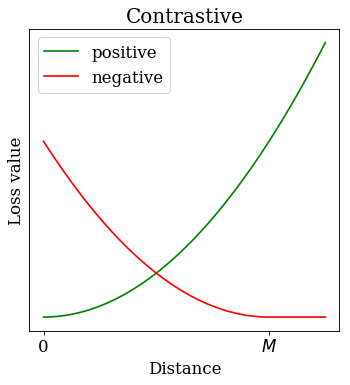
\includegraphics[width=0.48\textwidth]{Figures/contrastive.png}&
        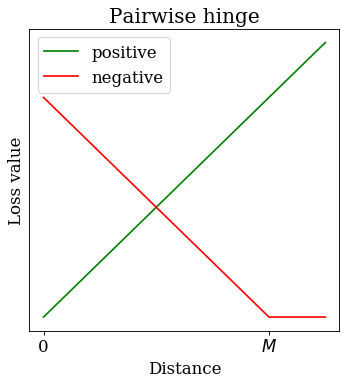
\includegraphics[width=0.48\textwidth]{Figures/pairwise_hinge.png}
    \end{tabular}
    \caption{The values of the Contrastive loss variants: (a) - \eq{contrastive}, (b) - \eq{coherence}. The losses are considered as functions of distance between a pair of image representations. The plots for positive and negative pairs are shown in green and red correspondingly.}
    \label{fig:contrastive}
\end{center}
\end{figure}
Contrastive loss has been first introduced in \citep{hadsell2006dimensionality} for dimensionality reduction and visualization. Later it was used for training a face recognition system in \citep{Sun14} in combination with the cross-entropy classification loss. For a pair of image descriptors $x_i$ and $x_j$ it is defined as:

%todo add more based i=on dimensionality reduction literature (LLE)
\begin{equation}
\label{eq:contrastive}
J_{contrastive}(x_i, x_j) = \begin{cases} \| x_i - x_j \|^{2}_{2}, & \text{if $(i,j)$ is a positive pair,} &\\  (\max(0, M - \| x_i - x_j \|_{2}))^2, & \text{if $(i,j)$ is a negative pair,}\end{cases}
\end{equation}
where $M$ is a hyperparameter, it defines a margin, or minimal distance for a negative pair that does not affect the loss value. In other words, it states when the non-matching examples are far enough and there is no need to push them farther.
The values of the Contrastive loss function for positive and negative pairs are shown in \fig{contrastive}a.

An analogous loss function, called Coherence loss or pairwise hinge loss, was utilized in \citep{mobahi2009deep} and \citep{Simo15} (see \fig{contrastive}b for the corresponding plots):
\begin{equation}
\label{eq:coherence}
J_{coherence}(x_i, x_j) = \begin{cases} \| x_i - x_j \|, & \text{if $(i,j)$ is a positive pair,} &\\  (\max(0, M - \| x_i - x_j \|)), & \text{if $(i,j)$ is a negative pair.}\end{cases}
\end{equation}

However, \citep{Lin15} show that forcing every positive pair to be represented by one point may lead to performance collapse, so the authors introduce the double-margin version of the loss function: 

\begin{equation}
\label{eq:double}
J_{double}(x_i, x_j) = \begin{cases} \max(0,\| x_i - x_j \|^{2}_{2} -M_1), & \text{if $(i,j)$ is a positive pair,} &\\  \max(0, M_2 - \| x_i - x_j \|_{2}^2), & \text{if $(i,j)$ is a negative pair,}\end{cases}
\end{equation}
where $M_1$ and $M_2$ are the two margin hyperparameters for positive and negative pairs correspondingly.\\\\


\bigskip\indent\textbf{Binomial Deviance loss}
 
\begin{figure}
\begin{center}
    \begin{tabular}{cc}
       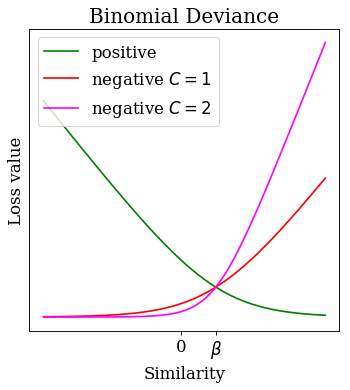
\includegraphics[width=0.48\textwidth]{Figures/bindev.png}&
        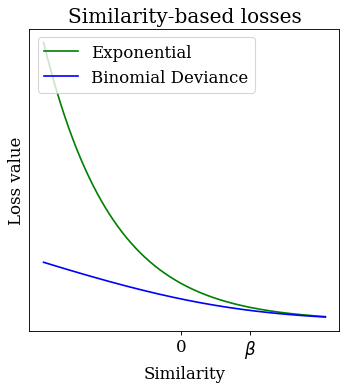
\includegraphics[width=0.48\textwidth]{Figures/similarity.png} \\
        (a) & (b)
    \end{tabular}
    \caption{(a) - the values of the Binomial Deviance loss \eq{bindev}. The plot for negative pairs is shown for $C=1$ and $C=2$, higher values of $C$ mean higher penalty for negative pairs violating the threshold $\beta$. (b) the values of the Binomial Deviance loss \eq{bindev} and the Exponential loss \eq{exp_sim_loss} for positive pairs. The losses are considered as functions of distance between a pair of image representations.}
    \label{fig:bindev}
\end{center}
\end{figure}

Binomial Deviance loss (generalized logistic loss) was considered in \citep{yi2014deep} for training a siamese neural network for person re-identification. Differently to Constrastive loss \eq{contrastive}, it is defined in terms of similarity for a pair of image descriptors. However, it should be noted, that the similar loss was also used in \citep{mignon2012pcca,hu2014discriminative}, but for Euclidean distance instead of cosine similarity. 

Binomial Deviance loss in defined as
\begin{equation}
\label{eq:bindev}
J_{dev}(s_{i,j}) = \ln (\exp^{-\alpha (s_{i,j}-\beta) m_{i,j}} +1 )\,,
\end{equation}
where $s_{i,j}$ is the cosine similarity measure between $i$th and $j$th examples, $\alpha$ and $\beta$ are the hyper-parameters. Furthermore,
$m_{i,j}$ differ for positive and negative pairs: % and scaling factors for the positive and negative pairs, so that:
\begin{align}
    \label{eq:bindev_weights}
    m_{i, j} = \left\{
	\begin{array}{l l}
		1, & \text{if $(i,j)$ is a positive pair,} & \\ 
	   -C, & \text{if $(i,j)$ is a negative pair,} &
	\end{array}\right.
% 	\\
%      w_{i, j}= \left\{
% 	\begin{array}{l l}
% 		\frac {1}{n_1}, & \text{if $(i,j)$ is a positive pair,} &\\
% 		\frac {1}{n_2}, & \text{if $(i,j)$ is a negative pair,} &
% 	\end{array}\right.
\end{align}	
%where $n_1$ and $n_2$ are the number of positive and negative pairs in the training set. 
The parameter $C$ is the negative cost for balancing weights for positive and negative pairs that was introduced in~\citep{yi2014deep}. The authors demonstrate that this parameter may influence the re-identification quality and results in better performance if tuned carefully.
The plots of the Binomial Deviance loss for different similarity values and different values of $C$ are shown in \fig{bindev}a. 

\citep{yi2014deep} have additionally considered the exponential similarity-based loss: 
% \begin{equation*}
%     J_{square}(s_{i,j}) = (s_{i,j} - l)^2,
% \end{equation*}

\begin{equation}
\label{eq:exp_sim_loss}
    J_{exp}(s_{i,j}) = \exp^{-\alpha (s_{i,j}-\beta) m_{i,j}}.
\end{equation}

The corresponding plots for different similarity-based losses are shown in \fig{bindev}b. 
The authors note that $J_{exp}$ \eq{exp_sim_loss} assigns a higher penalty value to the most violating pairs (\ie{} positive pairs with low similarity), whereas $J_{dev}$ \eq{bindev} is more robust to outliers. 

%todo write about classification on same-not same loss 
\citep{Li14, ahmed2015improved} also use binary cross-entropy for pairs of images as an objective. But instead of using a mapping from image to descriptor space first, they map a couple of images straight to the similarity score.

%todo find 2 papers based on comparing distributions


\begin{figure}
\begin{center}
    \begin{tabular}[t]{cc}
    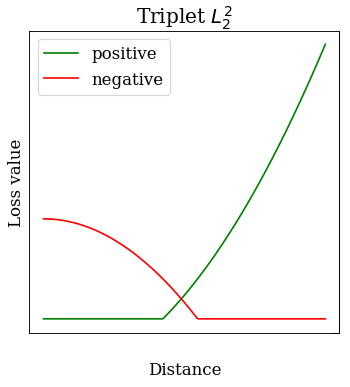
\includegraphics[width=0.48\textwidth]{Figures/triplet_l22.png}&
        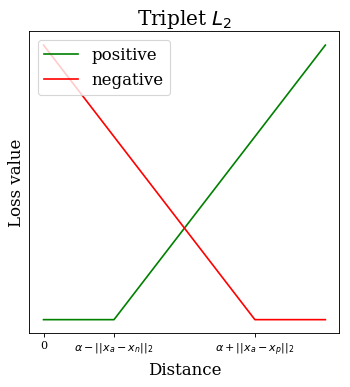
\includegraphics[width=0.48\textwidth]{Figures/triplet_l2.png} 
    \end{tabular}
    \caption{(a) plots the loss \eq{triplet}, (b) plots the loss \eq{triplet_l}. Green and red are for the loss as a function of $\|x_a - x_p \|_2$ and $\|x_a - x_n \|_2$ correspondingly (the other addend remains fixed).}
    \label{fig:triplet}
\end{center}
\end{figure}

\newpage
\bigskip\indent\textbf{Tripletwise losses}\\
\bigskip\indent\textbf{Triplet loss}

\citep{SchroffKP15} and \citep{parkhi2015deep} use the triplet loss (similar to \citep{weinberger2009distance}) for face verification:
\begin{equation}
\label{eq:triplet}
J_{triplet}^{L_2^2}(x_a,x_n,x_p)= \max(0, \alpha - \|x_a - x_n \|^2_{2} + \|x_a - x_p \|^2_{2})
\end{equation}

The loss is defined for a triplet of image representations $x_a$, $x_p$ and $x_n$, where $(x_a,x_p)$ is a positive pairs and $(x_a,x_n)$ is a negative pair. The idea of this loss is different to that of the pairwise losses: now we do not have any predefined threshold (or margin) that should separate all distances between positive pairs from all distances between negative pairs. In the triplet loss, such separation is learned independently for each anchor $x_a$. $\alpha$ is a hyperparameter that forces positive and negative distances to be additionally separated. 

\citep{SchroffKP15} also point out the problem of sampling the training triplets: it is important to select such triplets that violate the condition of the ordering of $x_p$ and $x_n$ in terms of distance to the anchor $x_a$:
\begin{equation*}
    \|x_a - x_p \|^2_{2} + \alpha <  \|x_a - x_n \|^2_{2}
\end{equation*}

In other words, the triplet affects the learning process if the corresponding loss value \eq{triplet} is positive. However, the authors also note that using the hardest (or most violating) triplets may lead to poor performance in practice. Therefore, the semi-hard sampling strategy was suggested. In more details, the triplet $(x_a, x_p, x_n)$ violating a margin $\alpha$ is considered to be semi-hard if the following condition is satisfied:
\begin{equation*}
    \|x_a - x_p \|^2_{2} <  \|x_a - x_n \|^2_{2}
\end{equation*}
Later, it was also shown in \citep{wu2017sampling} that the Contrastive loss \eq{contrastive} also benefits from utilizing this sampling scheme and the final results are on par with those of the triplet loss \eq{triplet}.

\citep{wu2017sampling} argue that the poor results of training using hardest examples come from the concave shape of the loss \eq{triplet} with respect to the distance between the negative pair $D_n = \|x_a - x_n \|_{2}$. The authors point out that the derivative of the loss with respect to $D_n$ is approaching zero for small values of $D_n$, which corresponds to hard triplets. At the same time the derivative of the loss with respect to $D_p = \|x_a - x_p \|_{2}$ remains large. This may lead to imbalance in handling positive and negative components and result in collapsing all representations to one point. \citep{wu2017sampling} suggest that this effect may be reduced by using the following loss function instead:
\begin{equation}
\label{eq:triplet_l}
J_{triplet}^{L_2}(x_a,x_n,x_p)= \max(0, \alpha - \|x_a - x_n \|_{2} + \|x_a - x_p \|_{2})
\end{equation}

The plots for the variants $J_{triplet}^{L_2^2}$ \eq{triplet} and $J_{triplet}^{L_2}$ \eq{triplet_l} are shown in \fig{triplet}.

\bigskip\indent\textbf{Lifted Structured Similarity Softmax loss}

The previously described loss functions are defined for separate pairs or triplets of training examples. The loss values for every such pair or triplet are averaged resulting in the final loss value. Differently from this scheme, \citep{Song16} define the loss function for a whole set of examples. In practice, the loss is calculated for all the examples in the training mini-batch. 

The idea of the \textit{Lifted Structured Similarity Softmax loss} (LSSS) suggested in \citep{Song16} is to take into account the hardest triplets. To make the loss function smooth, the logarithm of the sum of exponents is used. The LSSS loss is defined as follows: 

\begin{equation}
  \begin{aligned}
  \label{eq:lifted}
   J  = \tfrac{1}{2 \left| \mathcal{P} \right|} & \sum_{(i,j) \subseteq \mathcal{P}}  \max(0, \bar{J_{i,j}})^{2}, & \\
    \bar{J_{i,j}}  = \log(& \sum_{(i,k)\subseteq \mathcal{N}} \exp\{\alpha - \|x_i - x_k \|_2\} + &\\
   & \sum_{(j, l)\subseteq  \mathcal{N}}\exp\{\alpha -\|x_j - x_l \|_2\})  + \|x_i - x_j \|_2, & \\
  \end{aligned}
\end{equation}


where $\mathcal{P}$ and $\mathcal{N}$ are the sets of positive and negative pairs in the mini-batch, $\alpha$ is a hyperparameter.

The LSSS loss works with the batch of images and for each positive pair $(x_i, x_j)$ it samples all the related negative pairs $(x_i, x_k)$ and $(x_j, x_l)$. Thus, this approach is based on tripletwise learning. Another feature of this loss is that it is biased towards hard negatives.
%it also does something with mining

\bigskip\indent\textbf{N-pair loss}\\
\citep{sohn2016improved} introduce another loss function based on triplets. 

\begin{equation}
 \label{eq:npair}
 \begin{aligned}
    J_{N-pair}(\{x_i, x_i^+\}_i^N) = \frac1  N \sum_{i=1}^N  \log (1 + \sum_{i \neq j} \exp^{x_i\tran x_j^+ -x_i\tran x_i^+ })\\ = - \frac1  N \sum_{i=1}^N \log \frac {\exp^{x_i\tran x_i^+}}{\exp^{x_i\tran x_i^+} + \sum_{i \neq j} \exp^{x_i\tran x_j^+}}, 
\end{aligned}
\end{equation}
where $\{x_i, x_i^+\}_i^N$ - $N$ example pairs from $N$ different classes.
Similar to LSSS \eq{lifted}, it also uses triplet-based tuple structure where for each example pair multiple negatives are considered.


A similar loss (previously introduced in \citep{goldberger2005neighbourhood,globerson2006metric}), called Proxy-NCA loss, is used by \citep{movshovitz2017no}. The difference is that the positive and negative examples for triplets are replaced by learnable per-class proxies. This results in reduced number of triplets and alleviates the problem of sampling (choosing useful triplets for training). This loss is shown to outperform previously discussed triplet \eq{triplet}, LSSS \eq{lifted} and N-pair \eq{npair} losses.



\bigskip\indent\textbf{Quadruplet losses}
%todo mention that this was suggested simoultaneously or later than our work
%todo_minor: read how the classification problem s harder than verification?

The following loss function is suggested in \citep{Tadmor2016LearningAM} and \citep{wu2017sampling}:

\begin{equation}
\label{eq:margin}
J_{margin}(x_i, x_j) = \begin{cases}  \max(0,\alpha + (\| x_i - x_j \|_{2} - \beta)), & \text{if $(i,j)$ is a positive pair,} &\\  \max(0,\alpha - (\| x_i - x_j \|_{2} - \beta)), & \text{if $(i,j)$ is a negative pair,}\end{cases}
\end{equation}
Where $\alpha$ is a hyperparameter and $\beta$ is a learnable threshold separating the values of distances between positive and negative pairs. This loss is called \textit{margin-based} loss in  \citep{wu2017sampling}, so I follow this notation. Although this loss is defined for a pair of representations $(x_i, x_j)$, it is still related to the quadruplet learning, as the threshold $\beta$ is learned. Note, that the contrastive loss \eq{contrastive} does not allow to learn the margin parameter $M$ as it will converge to zero (the trivial solution). The margin-based loss \eq{margin} also resembles the double-margin contrastive loss \eq{double}.%it also has a trivial soulution if M1 and M2 are not the same!


%+sampling matters and quadruplet loss - the same? yes
%+why M should not be learned in contrastive, but okay for margin-based loss?: hypothesis: in "sampling matters" only  beta_class and beta_i are learned, b_0 remains fixed!- no the reason is that the same beta is used and therefore there is no trivial solution any more
%-+check the multibatch paper-+
%+how the sampling is practically done? - all positives are sampled, for each example in a positive pair, a negative pair is sampled according to the distance weighted sampling procedure.
%todo переделать графики триплето+


%todo say something about sampling
%TODO pcca and bin dev +


%\bigskip\indent\textbf{Other losses}
%center loss
%+ n pairs
%something about local structure?


%one problem is to choose good batches - example magnet loss
%another problem - to sample good examples inside the batch
%there are O(n^3) triplets so there should be more interations to cover all possible triplets, than fow example pairs, but it also has been shown that online sampling and distance reweighting helps triplet training.

%magnet loss uses the same idea of NCA loss, and also use some sort of proxies - clusters. also proxies are used by ProxyNCA and SoftTripleLoss

%softmax loss: it was shown that softmax and 

Besides the loss function choice, another important part of the training scheme is sampling. Hard-negative mining has been initially adopted by \citep{SchroffKP15} for triplet-based learning. Later has been also shown by \citep{wu2017sampling} that the results of contrastive \eq{contrastive} and margin \eq{margin} can be affected by the sampling scheme for negative examples. \citep{wu2017sampling} propose the distance-weighted sampling. \citep{movshovitz2017no}, however, avoid the sampling issue by introducing learnable proxies each of which is representing multiple training data points.



\section{CNN architectures for human recognition}
Several CNN-based methods for person re-identification have been proposed recently: \citep{Li14, yi2014deep, ahmed2015improved, chen2016deep, VariorHW16, VariorSLXW16,SuZX0T16}. 

\citep{yi2014deep} were among the first to build \textit{siamese} architectures that embeds of pedestrian images into the descriptor space, where they can be further compared using angular distance. 

In \citep{yi2014deep}, a peculiar architecture specific to pedestrian images is proposed that includes three independent sub-networks corresponding to three regions (legs, torso, head-and-shoulders). This is done in order to take into account the variability of the statistics of textures, shapes, and articulations between the three regions. %Our architecture includes the network of \citep{yi2014deep} as its part.

Apart from \citep{yi2014deep}, \citep{Li14} and \citep{ahmed2015improved} learn classification networks that can categorize a pair of images as either depicting  the same subjects or different subjects. In both approaches, the two images are fed into the network, and the difference in their mid-level representation is processed by additional special layers. Patch matching layer is used in \citep{Li14} and cross-input neighbourhood difference - in \citep{ahmed2015improved}). After that, extra convolutional and inner product layers are applied to the combined representation of the pair of images. Finally, the classification for the pair of images is performed using the softmax layer. The proposed deep learning approaches \citep{ahmed2015improved, yi2014deep, Li14}, while competitive, do not clearly outperform more traditional approaches based on ``hand-engineered'' features \citep{paisitkriangkrai2015learning, zhao2014person}.

When searching for matches in a dataset, the methods proposed in \citep{Li14}, \citep{ahmed2015improved} and \citep{chen2016deep} need to process pairs that include the query and every image in the dataset, and hence cannot directly utilize fast retrieval methods based on Euclidean and other simple distances. %Here we aim at the approach that can learn per-image descriptors and then compare them with cosine similarity measure. This justifies starting with the architecture proposed in  \citep{yi2014deep} and then modifying it by inserting new layers.
%TODO: VariorHW16, VariorSLXW16,SuZX0T16

Overall, the closest works to our approach described in \chapt{bilinear} are \citep{Yi14,cheng2016person} as they used separate streams to process horizontal stripes of the pedestrian image, both works consider $2$-depth convolutional streams.

The later work \citep{li2017learning} (after our work) use the same approach of multistream CNN (with a deeper $4$-layer architecture), but the authors additionally use Spatial Transformer Networks on each of the substreams, showing the results better than ours. Even better results were shown in \citep{zhao2017spindle}, where a special pose-predicting subnetwork is utilized to propose part-based regions for feature pooling.

\citep{saquib2018pose, suh2018part, kalayeh2018human} continue the idea of using the pose information explicitly. \citep{li2017learning} has a view point predictor as a part of architecture. \citep{suh2018part} and \citep{kalayeh2018human} incorporate sub-networks for pose prediction and semantic segmentation correspondingly.

%in 17 they started to use the pretrained networks!http://openaccess.thecvf.com/content_cvpr_2017/papers/Chen_Beyond_Triplet_Loss_CVPR_2017_paper.pdf http://openaccess.thecvf.com/content_cvpr_2018/papers/Sarfraz_A_Pose-Sensitive_Embedding_CVPR_2018_paper.pdf http://openaccess.thecvf.com/content_cvpr_2018/papers/Kalayeh_Human_Semantic_Parsing_CVPR_2018_paper.pdf http://openaccess.thecvf.com/content_cvpr_2018/papers/Chang_Multi-Level_Factorisation_Net_CVPR_2018_paper.pdf




\section{Multiplicative interactions of features}

\bigskip\ident\textbf{Covariance descriptor and second order pooling}\\
The multiplicative interactions between separate elements of feature vectors have been utilized for different visual recognition tasks. For example, 
the covariance descriptor has been introduced in \citep{tuzel2008pedestrian} for pedestrian detection and was further used for person re-identification and face verification in \citep{ma2012bicov}. 
The covariance descriptor of a region $R$ covering local features $X = \{x_i\}_1^S, x_i \in \mathbb{R}^d$ is defined as:
\begin{equation}
   \label{eq:covariance}
    C_R =\frac{1}{S-1} \sum_{i=1}^{S}(x_i-\mu)(x_i-\mu)\tran
\end{equation}
%compared with first order max and average pooling

Later, in  \citep{carreira2012semantic}, a similar operation has been used to pool the local descriptors in the context of semantic segmentation and classification.  %\citep{tuzel2008pedestrian} and \citep{carreira2012semantic} map the resulting features from the Riemannian manifold of symmetric positive definite matrices to the Euclidean tangent space before learning the final classifiers.

\bigskip\ident\textbf{Bilinear convolutional neural networks}\\
The Bilinear architecture suggested in \citep{lin2015bilinear} are much related to the two aforementioned approaches \citep{tuzel2008pedestrian,carreira2012semantic}). 

%todo fix
The bilinear operation is defined by \eq{bilinear}. It can be noticed that it performs a second-order pooling operation similar to \eq{covariance}.


Differently to \citep{tuzel2008pedestrian} and \citep{carreira2012semantic}, the features outer product is computed for two sets of local features $A$ and $B$ instead of one set of features $X$. The pooling is done over all the spatial locations, so the region $R$ in \eq{covariance} here corresponds to the whole featuremap.  The final architecture can be trained end-to-end which allows to fine-tune the feature extractors.

The Bilinear neural networks are also related to several popular feature aggregation techniques: BoVW \citep{csurka2004visual}, VLAD \citep{jegou2010aggregating} and Fisher Vector \citep{Perronnin10}. The reason is that these methods incorporate the encoding step. Each feature vector is encoded by a number of soft or hard assignments to the corresponding codes in the vocabulary. The resulting descriptor can be represented as an outer product of this encoding and the other part that is specific to the particular aggregation technique. The authors note that such encoding can be also viewed as part detectors. This analogy between the traditional feature aggregation approaches and the Bilinear architecture is described in details in  \citep{roychowdhury2015face}. The authors also show that the Bilinear architecture outperforms the Fisher Vector pooling applied to the local features extracted using a convolutional neural network.

Interestingly, the Bilinear neural networks are able to outperform other methods that rely on the part labeling, \eg{} \citep{branson2014bird}. It should be mentioned that the reported performance is on par with the performance of the Spatial Transformer Network \citep{jaderberg2015spatial}, that may learn the pose normalization without additional pose supervision.

Another important observation made in \citep{roychowdhury2015face} was about the performance of the Bilinear architecture for the birds species categorization. In turned out that the Bilinear architecture performs equally well for the initial images and for their tightly cropped versions. This is a piece of  evidence that the Bilinear model is able to implicitly learn to detect the important image parts.

The authors have initially suggested the Bilinear neural networks for fine-grained recognition problems. These type of recognition is characterized by high intra-category variations and low inter-category variations. The difficulty is that in some cases the intra-category variations may overcome the inter-category ones. For example, when recognizing the bird species, one should be able to take aside the pose and illumination variation an at the same time see the subtle differences in the beak shapes. 

The tasks of human recognition can also be described as fine-grained recognition. Moreover, the Bilinear neural networks have been successfully applied to face recognition with high pose variation in  \citep{lin2015bilinear}. Interestingly, in the latter, it was shown that the Bilinear architecture performs better than simple neural networks even without fine-tuning the feature extractors.  %the feature extractors 

After computing the outer products of the feature vectors, the dimensionality of the resulting feature is squared. This does not constitute a storage or computational problem when operating the low-dimensional features like \citep{tuzel2008pedestrian}, where $8$-length local descriptors were used resulting in the $64$-element covariance matrices. %what about bicov??
But for a large number of feature maps, the result of applying the bilinear operation \eq{bilinear} may be overwhelming. \citep{gao2016compact} address this problem by incorporating Random Maclaurin projection into the deep learning framework, which allows for the lower-dimensional results of the bilinear operation \eq{bilinear} with only a small performance drop.

Later (after the publication of the results of this work), \citep{suh2018part} has  also successfully approached person re-identification using Bilinear architecture. The two feature extractors explicitly model body part detection and appearance recognition: the former has been initialized by the pose detection model of \citep{cao2017realtime}, and the latter - is the GoogLeNet model \citep{szegedy2015going} pre-trained for classification.

%is not cited in introduction because they do not cite us
The latest work in \citep{kalayeh2018human} also applied similar a two-stream-multiplication approach to person re-identification (but is not considered as Bilinear by the authors). Like in the discussed works, one stream extracts appearance information. The other explicitly outputs probability maps for each of the semantic regions associated with different body parts. These maps are used as masks to pool the appearance features inside each semantic region.



\bigskip
\ident\textbf{Attention}\\
Another related line of work aims at explicitly modeling the attention mechanism of perceiving natural sentences and images. At a high level, this can also be described as learning "what" and "where" concepts and combining them using multiplication.

Initially, the simultaneous learning of the deep representations and the corresponding attention weights were introduced in the seminal work of \citep{BahdanauCB14} for neural machine translation. The goal is to encode the input sentence into a sequence of so-called annotation vectors and choose which of them to use (or attend) when generating the next word of the resulting translation. To perform this selection of annotation vectors, a set of corresponding weights is learned. This technique is developed to avoid encoding the whole sentence into a single vector, which leads to poor performance in some cases, \eg{} for long sentences. 

The following work of \citep{xu2015show} use the attention approach to learn visual attention maps for image captioning. \citep{BahdanauCB14} compute annotation vectors for a word sequence as activations of a bidirectional recurrent neural network, similarly, \citep{xu2015show} use a convolutional neural network to produce annotation vectors for a set of image locations.
%todo attention re-id
%todo: the paper citing the ours?

 %face, fine grained recognition

%todo : b-cnn for fine-grained recognition+
%       b-cnn compared to stns & other pose-based models+
%       VLAD FV BoW as bilinear model+-
%       faces with b-cnn: what to mention?-+


%todo other examples of factorization:
%     wavenet?
%gram matrices and style transfer?
%     attention+
%    covariance descriptor+
% todo: deep reid is also here!

\section{Domain adaptation} % and data augmentation

\bigskip\ident\textbf{Domain adaptation}\\
%todo add the notations  from pan2010survey to the introduction???
One popular direction in \textit{transfer learning} is \textit{domain adaptation}. This refers to a case when a  task is being solved for two different domains, as defined in \citep{pan2010survey}. The goal is to adapt the predictive algorithm trained on the labeled source data to the data in the target domain. %todo unsuperwised domain adaptation?

The common assumption in domain adaptation, called \textit{covariate shift} assumption, is that the difference between the two domains mainly comes from the difference in the feature distributions. In more details, under the \textit{covariate shift} assumption, only the marginal distributions of two domains differ, whereas the posterior probabilities of the labels in each domain coincide. This assumption also implies that the feature space is the same for the two domains. Under this assumption, the domain adaptation task is to make the domain marginal distributions closer to each other.   

%\textbf{Maximum Mean Discrepancy}

\citep{huang2007correcting, pan2008transfer, pan2011domain,baktashmotlagh2013unsupervised} estimate the domain distribution difference using Maximum Mean Discrepancy (MMD). The latter has been introduced in \citep{borgwardt2006integrating} to perform the comparison of two samples without the need to estimate the corresponding distributions (in a parametric or non-parametric way). The latter is achieved by utilizing a Reproducing Kernel Hilbert Space (RKHS) and the fact that squared MMD can be expressed in terms of the corresponding kernel function.

The empirical estimate of Maximum Mean Discrepancy is given by:
\begin{equation}
    \label{eq:MMD}
    MMD(X_\S, X_\T) = \| \frac{1}{n_{\S}} \sum_{i=1}^{n_{\S}} \phi \left(x^{\S}_i \right) - \frac{1}{n_{\T}} \sum_{i=1}^{n_{\T}} \phi \left(x^{\T}_i \right) \|_{\mathcal{H}},
\end{equation}
where $\{x^{\S}_i\}_{i=1}^{n_{\S}}$  and $\{x^{\T}_i\}_{i=1}^{n_{\T}}$ are the samples from the source and the target domains correspondingly, $\mathcal{H}$ is RKHS and $\phi$ is the corresponding feature mapping.

However, the mentioned works approach reducing the Maximum Mean Discrepancy differently.
\citep{huang2007correcting} use sample reweighting to choose the most 'useful' examples of the source domain. The idea is to reweight the exampled from the source domain in such a way that the expected risk (associated with the task being solved), for the reweighted source data will be equal to the expected risk for the target data. Such weights are given by $\beta(x,y) = \frac{ P_{\T}(x,y)}{P_{\S}(x,y)}$. And given the covariate shift assumption, $\beta(x) = \frac{ P_{\T}(x)}{P_{\S}(x)}$. To avoid estimating the domain distributions, the authors learn the weights $\beta$ by minimizing the empirical estimate of Maximum Mean Discrepancy between the target domain and the 'reweighted' source domain. 

Differently to \citep{huang2007correcting}, many other approaches seek the transformation of the source feature space (or source and target together) so that the source and target distributions match better. The point of such approaches is to extract the information that
is invariant across the source and target domains. 

\citep{pan2008transfer} aim at finding the lower dimensional space of features for this purpose, the method is called Maximum Mean Discrepancy Embedding. The motivation behind this approach is to get rid of those variation factors of the feature space that cause the marginal distributions of the domains to differ. The authors construct a semidefinite program in terms of the kernel matrix based on \eq{MMD} (with constraints ensuring that the distances between the nearest neighbors are preserved). PCA is then applied to the solution to get the final low-dimensional representations of the source and target examples. One disadvantage of this method is that it does not include any parametrization corresponding to a mapping onto the new feature space, therefore it cannot be used for the out-of-sample data. Such parametrization is introduced in the following work \citep{pan2011domain}, where the learning problem of \citep{huang2007correcting} is reformulated in terms of factorized and parametrized kernel matrix to enable the out-of-sample kernel evaluations. However, this causes the comparison of the sample means in a lower-dimension space rather than in Reproducing Kernel Hilbert Space. A somewhat similar approach correcting this drawback has been suggested in \citep{baktashmotlagh2013unsupervised}. In the latter, the MMD minimization is formulated in terms of the linear projection of the initial data, therefore an explicit transformation of the feature space is learned.

%golapan fernando is also here
While many approaches use Maximum Mean Discrepancy \eq{MMD}, another way of matching different domains is used in \citep{gong2012geodesic}. The authors model the gradual change between the domains. The two domains may have very different axes of variations, therefore the two d-dimensional subspaces, where the corresponding variances for each domain are maximized (\ie{} found using PCA), will be far from each other on the Grassmann manifold. The goal is to explore the intermediate subspaces on this manifold to extract the domain-invariant features. Moreover, the authors apply the kernel trick to take into account all the intermediate subspaces along the curve connecting the source and target domains. %is there any explicit mapping to a new feature space? yes it is shown in gong2013connecting (just square root of the kernel matrix)

The resampling technique similar to \citep{huang2007correcting} is utilized in \citep{gong2013connecting} in combination with the approach of \citep{gong2012geodesic}. The approach is based on the idea of solving multiple easier domain adaptation subtasks and then using their solutions as a basis for the final domain-invariant representation. Subtasks correspond different combinations of the examples in each of the two domains: to formulate each subtask, some examples are removed from the source domain and added to the target domain. Such examples are denoted \textit{landmarks} and are chosen by thresholding the results of sample reweighting (each subtask - with different kernel parameters). Therefore the examples from the source domain that are closest to the target domain are chosen in different ways. This allows to solve easier adaptation tasks, moreover, this gives multiple different perspectives on the initial task. The representations achieved by solving each of the subtasks are scaled and concatenated, and the scaling weights are learned discriminatively using the landmark examples and their labels.


\bigskip\ident\textbf{Deep domain adaptation}
%problem the re-id in the context of da is nor modelled

\bigskip\ident\textbf{Feature-level domain adaptation.} Like many of the above-mentioned methods, deep learning methods for domain adaptation aim at learning a data representation that would be the best at explaining both domains simultaneously. However, deep learning gives the tools for learning such features at multiple levels, whereas non-deep techniques work with data descriptions that are fixed and extracted beforehand. Deep learning methods, in contrast, are able to work with the raw input and extract a hierarchy of features. Thus, like for many other recognition tasks, multiple successful deep learning methods have been suggested for domain adaptation. 

One of the first deep domain adaptation methods was suggested in \citep{glorot2011domain} for sentiment analysis. The Denoising Autoencoder \citep{vincent2008extracting} is trained on the mixed data from both domains to capture their common concepts. Like in the non-deep approaches, described above, the transformed labeled data are then used for training the final domain-invariant classifier.

\citep{chopra2013dlid} combines the ideas of \citep{gong2012geodesic} and \citep{glorot2011domain} to propose a deep learning framework interpolating between the two domains. Unlike \citep{glorot2011domain}, both the task-specific prediction algorithm and domain-invariant feature extractors are neural networks. This allows finetuning the parameters of both these parts simultaneously by propagating the gradients from the task-specific network to the feature extractors. The gradual change between the domains is modeled by constructing multiple variants of the mixture of the two domains: different proportions of the data from the two domains are used. Each of the feature extractors is trained in an unsupervised manner using one of such mixtures. The final representation is composed as a concatenation of outputs of all of these feature extractors.

Finally, \citep{LongC0J15} suggest a deep neural network, called DAN (Deep Adaptation
Network), that is trained with the two objectives: one is a task-specific loss and another is to match the distributions of the two domains using Maximum Mean Discrepancy \eq{MMD}. The matching is performed for several higher-level layers of the main neural network to ensure that the domains are aligned well, as the last layers of a neural network are considered to be the most domain-specific ones. \citep{tzeng2014deep} similarly use \eq{MMD} as an additional objective to train a domain-invariant neural network. In the latter, the authors use only one layer for matching the domain distributions. This layer is chosen among the last layers of the neural network so that the corresponding MMD value is minimized.

Notably, the deep approaches of \citep{chopra2013dlid, tzeng2014deep, LongC0J15} outperform the previous non-deep methods, \eg{} the strong method of \citep{gong2012geodesic}, by a large margin on the cross-domain classification.
%todo which of them are better? compared to non-deep?

\bigskip\ident\textbf{Image-level domain adaptation.}
%to do last layers are
%this is extracted from da face paper
%todo: rewrite ?
%model
Since the CycleGAN \citep{ZhuPIE17} architecture for image-to-image translation and stylization appeared, domain adaptation has become one of its active fields of application. This approach differs from the feature-level domain adaptation techniques of \citep{LongC0J15} and \citep{tzeng2014deep} or the method presented in the \chapt{gradrev}, because rather than finding deep domain-invariant representations, it works on the pixel level and aims at building mappings between the image domains. Thus the domain adaptation is done in two steps: building a mapping the source domain to target and retraining the predictor on the transferred source data. (Although it is also possible to combine these two steps into one optimization process.)%cycada


The methods of \citep{Hoffman17,Deng_2018_CVPR,Murez_2018_CVPR} employ CycleGAN framework to change the domain of training data for various tasks, including classification, segmentation, and person re-identification. 

%pedestrians
In particular, for person re-identification, the pixel-level domain adaptation with CycleGAN has been applied in several recent works \citep{zhong2018camera, Deng_2018_CVPR} (after the results of the \chapt{gradrev} were published). Some of them consider different datasets as domains, others aim at utilizing synthetic re-identification data to improve the results on real data \citep{bak2018domain}. As demonstrated by these works, image-to-image translation may help a lot to overcome the visual (\eg{} caused by different illumination) differences between the source and target camera sets.


 \citep{HongIRY17} and
 \citep{SohnLZY0C17} approach face recognition tasks for low-quality image domain. They consider image degradation as a domain shift and perform feature-level unsupervised domain adaptation based on adversarial learning showing better recognition results. 
In works \citep{HongIRY17} and \citep{SohnLZY0C17} it is shown that domain-specific data augmentation is essential for training face recognition systems. 
 However, in both works, the data augmentation is performed 'by hand' (the degradation types and hyper-parameters for transforms are chosen and fixed).%, while we augment the training data in an automatic manner utilizing the CycleGAN framework, which can also be viewed as an image-level domain adaptation.
%Additionally, in contrast to \citep{HongIRY17}, we do not consider extremely large pose variation. Instead, we are more focused on the image degradation factors (e.g. the combination of small size, blur, JPEG-compression). 
%Differently from \citep{SohnLZY0C17}, where evaluation is performed for the Youtube faces dataset, we approach the task in the presence of the somewhat stronger domain shift, as our test data are captured by surveillance cameras and are mostly of much lower quality.


%\subsection{Adversarial learning for augmentation}

%todo in hist loss check the @cumber@ problem if there are too many bins (and some are empty)

\newpage 
\newcommand{\histroot}{Chapters/histloss}

\chapter{Learning Deep Embeddings with Histogram Loss}
\label{chapt:hist}
 


%todo something about the importance of the loss function compared to architecture from israel paper?
\section{Motivation}
%: objective functions for similarity learning

% The problem of learning deep embeddings is considered in this chapter. Usually, such learning is performed using siamese architectures described in  \sect{intro_siamese} to solve the similarity estimation \pr{similarity_estimation}. Under this approach, complex input patterns (\eg{} images) are mapped into a high-dimensional space through a chain of feed-forward transformations, while the parameters of the transformations are learned from a large amount of supervised data. The \textit{objective} of the learning process is to achieve the proximity of semantically related patterns (\eg{} images of the same person) and avoid the proximity of semantically unrelated (\eg{} images of different people) in the target space. It should be noted that this work is focused on simple similarity measures such as Euclidean distance or scalar products, as they allow fast evaluation.

% The formulation of an objective function for learning embeddings depends on the exact formulation of \pr{similarity_estimation}. It can be formalized in several different ways depending on the setting: 
% \begin{enumerate}
% \item \label{assumption_1} whether we need all the positive pairs to have higher similarity values than \textit{all} the negative pairs,

% \item \label{assumption_2} or we only need this condition fulfilled for each separate identity. 
% \end{enumerate}

In more detail, the latter means that positive pairs ${(x_i^a, x_j^a)}_{i,j}$ that consist of images of some identity $a$ should have the higher similarity value compared only to corresponding negative pairs ${(x_i^a, x_k^{n})}_{i,k}$, that contain one image for the identity $a$ and the second image - for some other identity $n$. 

According to one of the two described assumptions, the training data for the similarity-learning tasks may be formed in one of the following basic ways:

\begin{itemize}
    \item a set of positive pairs and a set of negative pairs:
        \begin{equation}
          \begin{aligned}
          \label{c:pairs_constraints}
                   S = \{(x_i^a, x_j^a): x_i^a \text{ and }& x_j^a \text{ are similar}\}, & \\
                   D = \{(x_i^b, x_j^c): x_i^b \text{ and }& x_j^c \text{ are not similar}\};&\\
          \end{aligned}
        \end{equation}

     
    \item a set of triplets:
     \begin{equation}
     \label{c:triplets_constraints}
          R = \{(x_i^a, x_j^a, x_k^n): x_i^a \text{ is more similar to } x_j^p \text{ than to } x_k^n\}; 
     \end{equation}
     
     \item a set of quadruplets:
     \begin{equation}
         \label{c:quadruplets_constraints}
          Q = \{(x_i^a, x_j^a, x_k^b, x_l^c): x_i^a \text{ and } x_j^a \text{ are more similar than } x_k^b \text{ and } x_l^c\}.
      \end{equation}
\end{itemize}

\bigskip\textbf{Training with pairs and quadruplets}\\
The training data forms \ref{c:pairs_constraints} and \ref{c:quadruplets_constraints} correspond to the assumption \ref{assumption_1}. The pairwise data \ref{c:pairs_constraints} require comparing the similarity of each pair to some pre-defined threshold in the process of training (such threshold should separate similarity values of positive and negative pairs). The using of quadruplet data \ref{c:quadruplets_constraints} usually implies comparing the similarity values between the independent pairs (so no predefined threshold is necessary). While pairwise data case is more rigid and requires more assumptions about the data (the threshold value), handling of quadruplet data  is more computationally expensive (number of comparisons will be quadratic in the number of pairs).
%examples

The pairwise form of training data is widely used in metric learning \citep{xing2003distance,globerson2006metric,davis2007information,koestinger2012large,liao2015person,mignon2012pcca}, and also for training siamese architectures by \citep{Bromley93,hadsell2006dimensionality}, including those for face verification by \citep{Sun14, hu2014discriminative} and person re-identification by \citep{yi2014deep, Yi14}.

Quadruplet-based learning is less popular. The metric learning method of \citep{law2013quadruplet} is one of the examples under this category. 
The loss function suggested by \citep{Tadmor2016LearningAM} (it was published simultaneously with the corresponding results of this work) on deep face verification can also be considered quadruplet-based. The reason is that the threshold for separating similarities of positive and negative pairs is a learned parameter in this work. 


\bigskip\textbf{Training with triplets}\\
The triplet form of training data \ref{c:triplets_constraints} corresponds to the assumption \ref{assumption_2}. Differently to pairwise \ref{c:pairs_constraints} and quadruplet data \ref{c:quadruplets_constraints}, for triplets, only relative similarities/distances are compared. This means that the neighborhoods corresponding to different training classes are allowed to be of a different radius in the descriptor space. This is in contrast to using pairs and quadruplets, which implies that all distance (negative similarity) value for positive pairs should not exceed a  certain threshold. 

Training data organized as triplets are usually used for ranking formulations: either linear ranking functions like in methods by
\citep{joachims2002optimizing,prosser2010person,kuo2013person,paisitkriangkrai2015learning} or non-linear ranking functions parametrized by CNN \citep{chen2016deep}. Triplet-based approach is also used for metric learning \citep{schultz2004learning,weinberger2009distance}, and for training siamese neural networks for re-identification \citep{Song16} and even for the verification formulation of the face recognition problem \citep{SchroffKP15,parkhi2015deep}. 
%something about sampling?? but it is also important for pairwise losses, so it probably should not be mentioned
%maybe computational complexity?

\bigskip\textbf{Classification objective}\\
%from the histloss paper
It has been observed in \citep{Krizhevsky12} and confirmed later in multiple works (\eg{} \citep{Razavian14}) that deep networks trained for classification can be used for deep embedding. In particular, it is sufficient to consider an intermediate representation arising in one of the last layers of the deep network. In human recognition task, identity numbers can be used as class labels in order to apply the classification training. \citep{Taigman14} dramatically improved the results for face verification using the classification objective for training a CNN. \citep{parkhi2015deep} use pre-training for classification followed by triplet-based training for the same task. 

Overall, using classification objectives can help the final results \citep{Sun14}, however, this work considers objective functions that are specially designed for learning deep embeddings. 

\bigskip\indent\textbf{Sampling}\\
It has been later demonstrated in literature \citep{sohn2016improved, wu2017sampling}, that sampling scheme for training tuples may be very important and can affect the results. In this chapter, we, however, use simple sampling: we generate all the possible pairs within the mini-batch.



%using pre-trained on imagenet networks? face , re-id, instance retrieval? paper ME (pretrained CNN features are bad for reid?)

%tell what is bad about triplets? computational complexity?
\bigskip\textbf{Motivation for a new loss function}\\
As it was mentioned in the several last paragraphs, the training objectives for embedding learning are most often based on using point-wise constraints \ref{c:pairs_constraints}, \ref{c:triplets_constraints}, \ref{c:quadruplets_constraints}. 
This leads to 
\begin{itemize}
    \item either presence of hyperparameters, (like thresholds, whose optimal values can vary for different training datasets),
    \item or using more complex structures of training data (like triplets or quadruplets).
\end{itemize}  

In this chapter a new loss function that helps to avoid both of these issues is suggested. In designing this function we strive to avoid highly-sensitive parameters such as margins or thresholds of any kind. While processing a batch of data points, the proposed loss is computed in two stages. 
\begin{enumerate}
\item Firstly, the two one-dimensional distributions of similarities in the embedding space are estimated, one corresponding to similarities between matching (\textit{positive}) pairs, the other corresponding to similarities between non-matching (\textit{negative}) pairs. The distributions are estimated in a simple non-parametric way (as histograms with linearly-interpolated values-to-bins assignments).
\item In the second stage, the overlap between the two distributions is computed by estimating the probability that the two points sampled from the two distribution are in a wrong order, i.e.\ that a random negative pair has a higher similarity than a random positive pair.
\end{enumerate}

It should be noted that the way of estimating the overlap between the similarity distributions in the second stage is quite important. The reason we choose the reverse order probability described above is that this loss forces the similarity distribution for positive pairs to the right and the distribution for negative pairs - to the left with respect to the similarity value axis. The latter means that during the process of training, each positive pair gets a pulling signal and each negative pair - a repelling signal. For such measures as Kullback-Leibler divergence \citep{kullback1951information} or Bhattacharyya distance \citep{bhattacharyya1943measure}, this may not be a case, especially if the similarity distributions given by untrained network are highly overlapping. The problem is that, in contrast to the suggested method, these measures do not imply the ordering of distribution means. However, it should be noted that this problem could be fixed by introducing an additional optimization objective, \eg{} the difference between means of the two distributions. 



The two stages are implemented in a piecewise-differentiable manner, thus allowing to minimize the loss (i.e.\ the overlap between distributions) using standard backpropagation.
The number of bins in the histograms is the only tunable parameter associated with our loss, and it can be set according to the batch size independently of the data itself. In the experiments, we fix this parameter (and the batch size) and demonstrate the versatility of the loss by applying it to four different image datasets of varying complexity and nature. Comparing the new loss to state-of-the-art reveals its favorable performance. Overall, we hope that the proposed loss will be used as an ``out-of-the-box'' solution for learning deep embeddings that requires little tuning and leads to close to the state-of-the-art results.


% \begin{abstract}
% We suggest a loss for learning deep embeddings. The new loss does not introduce parameters that need to be tuned and results in very good embeddings across a range of datasets and problems. The loss is computed by estimating two distribution of similarities for positive (matching) and negative (non-matching) sample pairs, and then computing the probability of a positive pair to have a lower similarity score than a negative pair based on the estimated similarity distributions. We show that such operations can be performed in a simple and piecewise-differentiable manner using 1D histograms with soft assignment operations. This makes the proposed loss suitable for learning deep embeddings using stochastic optimization. In the experiments, the new loss performs favourably compared to recently proposed alternatives. 
% \end{abstract}



% %-------------------------------------------------------------------------
% \section{Introduction}

% Deep feed-forward embeddings play a crucial role across a wide range of tasks and applications in image retrieval \citep{Krizhevsky12,Razavian14,Arandjelovic15}, biometric verification \citep{Bromley93,Chopra05,Taigman14,Sun14,Schroff15,parkhi2015deep,Yi14}, visual product search \citep{Song16}, finding sparse and dense image correspondences \citep{Simo15,Zbontar15}, etc. Under this approach, complex input patterns (\eg{} images) are mapped into a high-dimensional space through a chain of feed-forward transformations, while the parameters of the transformations are learned from a large amount of supervised data. The \textit{objective} of the learning process is to achieve the proximity of semantically-related patterns (\eg{} faces of the same person) and avoid the proximity of semantically-unrelated (\eg{} faces of different people) in the target space. In this work, we focus on simple similarity measures such as Euclidean distance or scalar products, as they allow fast evaluation, the use of approximate search methods, and ultimately lead to faster and more scalable systems. 

% Despite the ubiquity of deep feed-forward embeddings, learning them still poses a challenge and is relatively poorly understood. While it is not hard to write down a loss based on tuples of training points expressing the above-mentioned objective, optimizing such a loss rarely works ``out of the box'' for complex data. This is evidenced by the broad variety of losses, which can be based on pairs, triplets or quadruplets of points, as well as by a large number of optimization tricks employed in recent works to reach state-of-the-art, such as pretraining for the classification task while restricting fine-tuning to top layers only~\citep{Taigman14,parkhi2015deep}, combining the embedding loss with the classification loss~\citep{Sun14}, using complex data sampling such as mining ``semi-hard'' training triplets \citep{Schroff15}. Most of the proposed losses and optimization tricks come with a certain number of tunable parameters, and the quality of the final embedding is often sensitive to them.

% Here, we propose a new loss function for learning deep embeddings. In designing this function we strive to avoid highly-sensitive parameters such as margins or thresholds of any kind. While processing a batch of data points, the proposed loss is computed in two stages. Firstly, the two one-dimensional distributions of similarities in the embedding space are estimated, one corresponding to similarities between matching (\textit{positive}) pairs, the other corresponding to similarities between non-matching (\textit{negative}) pairs. The distributions are estimated in a simple non-parametric ways (as histograms with linearly-interpolated values-to-bins assignments). In the second stage, the overlap between the two distributions is computed by estimating the probability that the two points sampled from the two distribution are in a wrong order, i.e.\ that a random negative pair has a higher similarity than a random positive pair. The two stages are implemented in a piecewise-differentiable manner, thus allowing to minimize the loss (i.e.\ the overlap between distributions) using standard backpropagation. The number of bins in the histograms is the only tunable parameter associated with our loss, and it can be set according to the batch size independently of the data itself. In the experiments, we fix this parameter (and the batch size) and demonstrate the versatility of the loss by applying it to four different image datasets of varying complexity and nature. Comparing the new loss to state-of-the-art reveals its favourable performance. Overall, we hope that the proposed loss will be used as an ``out-of-the-box'' solution for learning deep embeddings that requires little tuning and leads to close to the state-of-the-art results.
% %---------------------------------------

\begin{figure}
    \centering
    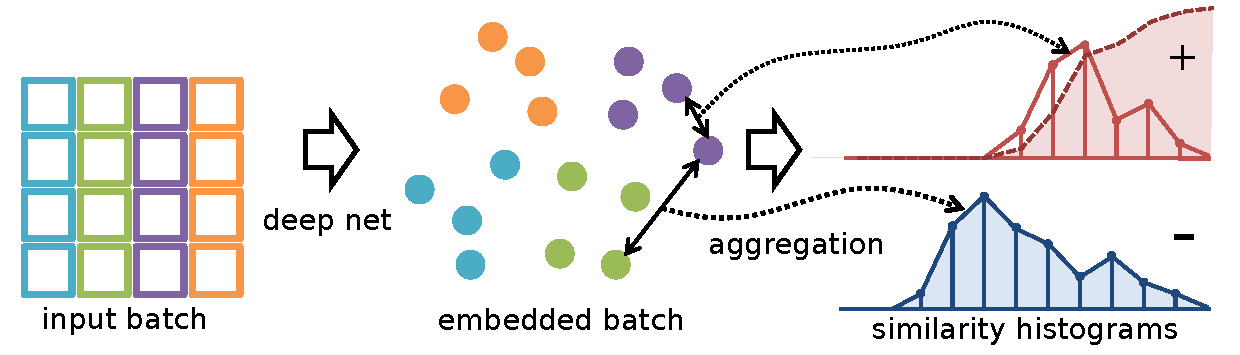
\includegraphics[width=\textwidth]{\histroot/figures/nPLoss.pdf}
    \caption{The histogram loss computation for a batch of examples 
    (color-coded; same color indicates matching samples). After the batch (left) is embedded into a high-dimensional space by a deep network (middle), we compute the histograms of similarities of positive (top-right) and negative pairs (bottom-right). We then evaluate the integral of the product between the negative distribution and the cumulative density function for the positive distribution (shown with a dashed line), which corresponds to a probability that a randomly sampled positive pair has smaller similarity than a randomly sampled negative pair. Such histogram loss can be minimized by backpropagation. The only associated parameter of such loss is the number of histogram bins, to which the results have very low sensitivity.}
    \label{fig:scheme}
\end{figure}


% \section{Related work}

% Recent works on learning embeddings use deep architectures (typically ConvNets \citep{LeCun89,Krizhevsky12}) and stochastic optimization. Below we review the loss functions that have been used in recent works.% Overall, previous works consider mapping from input patterns to a unit sphere in a high-dimensional space (normalized descriptors). Normalization to a unit length has been invariably reported to improve the performance both for deep and for ``shallow'' embeddings \citep{Perronnin10}. The training points are assumed to come with some sort of supervision, typically with class labels, so that for any pair of samples it is known whether they should end up close in the embedding space (positive pair) or whether they should be separated by some distance (negative pair). Some loss functions (including ours) can be extended to a weaker form of supervision, where ``same'' or ``different'' relations are known for only subset of pairs.

% {\bf Classification losses.} It has been observed in \citep{Krizhevsky12} and confirmed later in multiple works (\eg{} \citep{Razavian14}) that deep networks trained for classification can be used for deep embedding. In particular, it is sufficient to consider an intermediate representation arising in one of the last layers of the deep network. The normalization is added post-hoc. Many of the works mentioned below pre-train their embeddings as a part of the classification networks.

% {\bf Pairwise losses.} Methods that use pairwise losses sample pairs of training points and score them independently. The pioneering work on deep embeddings \citep{Bromley93} penalizes the deviation from the unit cosine similarity for positive pairs and the deviation from $-1$ or $-0.9$ for negative pairs.
% Perhaps, the most popular of pairwise losses is the \textit{contrastive} loss \citep{Chopra05,Simo15}, which minimizes the distances in the positive pairs and tries to maximize the distances in the negative pairs as long as these distances are smaller than some margin $M$. Several works pointed to the fact  that attempting to collapse all positive pairs may lead to excessive overfitting and therefore suggested losses that mitigate this effect, \eg{} a double-margin contrastive loss \citep{Lin15}, which drops to zero for positive pairs as long as their distances fall beyond the second (smaller) margin. Finally, several works use non-hinge based pairwise losses such as log-sum-exp and cross-entropy on the similarity values that softly encourage the similarity to be high for positive values and low for negative values (\eg{} \  \citep{Yi14,Taigman14}). The main problem with pairwise losses is that the margin parameters might be hard to tune, especially since the distributions of distances or similarities can be changing dramatically as the learning progresses. While most works ``skip'' the burn-in period by initializing the embedding to a network pre-trained for classification \citep{Taigman14}, \citep{Sun14} further demonstrated the benefit of admixing the classification loss during the fine-tuning stage (which brings in another parameter).

% {\bf Triplet losses.} While pairwise losses care about the absolute values of distances of positive and negative pairs, the quality of embeddings ultimately depends on the relative ordering between positive and negative distances (or similarities). Indeed, the embedding meets the needs of most practical applications as long as the similarities of positive pairs are greater than similarities of negative pairs \citep{Schultz04,Weinberger09}. The most popular class of losses for metric learning therefore consider triplets of points $x_0,x_+,x_-$, where $x_0,x_+$ form a positive pair and $x_0,x_-$ form a negative pair and measure the difference in their distances or similarities. Triplet-based loss can then \eg{} be aggregated over all triplets using a hinge function of these differences. Triplet-based losses are popular for large-scale embedding learning \citep{Chechik10} and in particular for deep embeddings~\citep{parkhi2015deep,Schroff15,Qian15,Zbontar15,Song16}. Setting the margin in the triplet hinge-loss still represents the challenge, as well as sampling ``correct'' triplets, since the majority of them quickly become associated with zero loss. On the other hand, focusing sampling on the hardest triplets can prevent efficient learning \citep{Schroff15}. Triplet-based losses generally make learning less constrained than pairwise losses. This is because for a low-loss embedding, the characteristic distance separating positive and negative pairs can vary across the embedding space (depending on the location of $x_0$), which is not possible for pairwise losses. In some situations, such added flexibility can increase overfitting.

% {\bf Quadruplet losses.} Quadruplet-based losses are similar to triplet-based losses as they are computed by looking at the differences in distances/similarities of positive pairs and negative pairs. In the case of quadruplet-based losses, the compared positive and negative pairs do not share a common point (as they do for triplet-based losses). Quadruplet-based losses do not allow the flexibility of triplet-based losses discussed above (as they includes comparisons of positive and negative pairs located in different parts of the embedding space). At the same time, they are not as rigid as pairwise losses, as they only penalize the relative ordering for negative pairs and positive pairs. Nevertheless, despite these appealing properties, quadruplet-based losses remain rarely-used and confined to ``shallow'' embeddings \citep{Law13,Zheng13}. We are unaware of deep embedding approaches using quadruplet losses. A potential problem with quadruplet-based losses in the large-scale setting is that the number of all quadruplets is even larger than the number of triplets. Among all groups of losses, our approach is most related to quadruplet-based ones, and can be seen as a way to organize learning of deep embeddings with a quarduplet-based loss in an efficient and (almost) parameter-free manner.


%---------------------------------------
\section{Histogram loss}
\label{sect:loss}

We now describe our loss function and then relate it to the quadruplet-based loss. Our loss (\fig{scheme}) is defined for a batch of examples $X = \{x_1,x_2,\dots x_N\}$ and a deep feedforward network $f(\cdot;\theta)$, where $\theta$ represents learnable parameters of the network. We assume that the last layer of the network performs length-normalization, so that the embedded vectors $\{y_i = f(x_i;\theta)\}$ are $L2$-normalized.

We further assume that we know which elements should match to each other and which ones are not. Let $m_{ij}$ be $+1$ if $x_i$ and $x_j$ form a positive pair (correspond to a match) and $m_{ij}$ be $-1$ if $x_i$ and $x_j$ are known to form a negative pair  (these labels can be derived from class labels or be specified otherwise). Given $\{m_{ij}\}$ and $\{y_i\}$ we can estimate the two probability distributions $\prp$ and $\prm$ corresponding to the similarities in positive and negative pairs respectively. In particular $\Sp = \{ s_{ij} = \spr{x_i}{x_j}\,|\,m_{ij} = +1\}$ and $\Sm = \{s_{ij} = \spr{x_i}{x_j}\,|\,m_{ij} = -1\}$ can be regarded as sample sets from these two distributions. Although samples in these sets are not independent, we keep all of them to ensure a large sample size. 

Given sample sets $\Sp$ and $\Sm$, we can use any statistical approach to estimate $\prp$ and $\prm$. The fact that these distributions are one-dimensional and bounded to $[-1;+1]$ simplifies the task. Perhaps, the most obvious choice in this case is fitting simple histograms with uniformly spaced bins, and we use this approach in our experiments. We therefore consider $R$-dimensional histograms $\Hp$ and $\Hm$, with the nodes $t_1=-1,t_2,\dots,t_R=+1$ uniformly filling $[-1;+1]$ with the step $\Delta=\frac{2}{R-1}$. We estimate the value $\hp_r$ of the histogram $\Hp$ at each node as:
\begin{equation} \label{eq:hist}
    \hp_r = \frac{1}{|\Sp|}\sum_{(i,j)\,:\,m_{ij}=+1} \delta_{i,j,r}\, 
\end{equation}
where $(i,j)$ spans all positive pairs of points in the batch. The weights $\delta_{i,j,r}$ are chosen so that each pair sample is assigned to the two adjacent nodes:
\begin{equation} \label{eq:histweight}
\delta_{i,j,r} = \begin{cases} 
    (s_{ij}-t_{r-1})/\Delta,\; &\text{if $s_{ij} \in [t_{r-1};t_r]$},\\
    (t_{r+1}-s_{ij})/\Delta,\; &\text{if $s_{ij} \in [t_r;t_{r+1}]$},\\
    0,\; &\text{otherwise}\,.
    \end{cases}
\end{equation}
 We thus use linear interpolation for each entry in the pair set, when assigning it to the two nodes. The estimation of $\Hm$ proceeds analogously. Note, that the described approach is equivalent to using ''triangular'' kernel for density estimation; other kernel functions can be used as well. %\citep{GVK233599487}.

Once we have the estimates for the  distributions $\prp$ and $\prm$, we use them to estimate the probability of the similarity in a random negative pair to be more than the similarity in a random positive pair ( \textit{the probability of reverse}). Generally, this probability can be estimated as:
\begin{equation} \label{eq:reverse}
p_\text{reverse} = \int_{-1}^{1} \prm(x) \left[\int_{-1}^x \prp(y)\,dy\right]\, dx \, =
\int_{-1}^{1} \prm(x)\,\Phi^{+}(x)\, dx = \mathbb{E}_{x \sim \prm}[\Phi^{+}(x)]\,,
\end{equation}
where $\Phi^{+}(x)$ is the CDF (cumulative density function) of $\prp(x)$. The integral \eq{reverse} can then be approximated and computed as:
\begin{equation} \label{eq:loss}
L(X,\theta) = \sum_{r=1}^R \left( \hm_r \sum_{q=1}^r \hp_q  \right)= \sum_{r=1}^R  \hm_r \phi^{+}_r\,,
\end{equation}
where $L$ is our loss function (the \textit{histogram loss}) computed for the batch $X$ and the embedding parameters $\theta$, which approximates the reverse probability; $\phi^{+}_r=\sum_{q=1}^r \hp_q$ is the cumulative sum of the histogram $\Hp$.

Importantly, the loss \eq{loss} is differentiable w.r.t.\ the pairwise similarities $s\in\Sp$ and $s\in\Sm$. Indeed, it is straightforward to obtain $\frac{\partial L}{\partial \hm_r} = \sum_{q=1}^{r} \hp_q$ and $\frac{\partial L}{\partial \hp_r}=\sum_{q=r}^{R} \hm_q$ from \eq{loss}. Furthermore, from \eq{hist} and \eq{histweight} it follows that:
\begin{equation} \label{eq:histder}
\frac{\partial \hp_r}{\partial s_{ij}} = \begin{cases} 
     \frac{+1}{\Delta |\Sp|} ,\; &\text{if $s_{ij} \in [t_{r-1};t_r]$},\\
     \frac{-1}{\Delta |\Sp|},\; &\text{if $s_{ij} \in [t_r;t_{r+1}]$},\\
    0,\; &\text{otherwise}\,,
    \end{cases}
\end{equation}
for any $s_{ij}$ such that $m_{ij}=+1$ (and analogously for $\frac{\partial \hm_r}{\partial s_{ij}}$). Finally, $\frac{\partial s_{ij}}{\partial x_i}=x_j$ and $\frac{\partial s_{ij}}{\partial x_j}=x_i$. One can thus backpropagate the loss to the scalar product similarities, then further to the individual embedded points, and then further into the deep embedding network.

{\bf Relation to quadruplet loss.} \\
Our loss first estimates the probability distributions of similarities for positive and negative pairs in a semi-parametric ways (using histograms), and then computes the probability of reverse using these distributions via equation \eq{loss}. An alternative and purely non-parametric way would be to consider all possible pairs of positive and negative pairs contained in the batch and to estimate this probability from such set of pairs of pairs. This would correspond to evaluating a quadruplet-based loss similarly to \citep{Law13,Zheng13}. The number of pairs of pairs in a batch, however tends to be quartic (fourth degree polynomial) of the batch size, rendering exhaustive sampling impractical. This is in contrast to our loss, for which the separation into two stages brings down the complexity to quadratic in batch size. Another efficient loss based on quadruplets is introduced in \citep{Tadmor2016LearningAM}. The training is done pairwise, but the threshold separating positive and negative pairs is also learned.

We note that quadruplet-based losses as in \citep{Law13,Zheng13} often encourage the positive pairs to be more similar than negative pairs by some non-zero margin. It is also easy to incorporate such non-zero margin into our method by defining the loss to be:
\begin{equation} \label{eq:margin}
L_\mu(X,\theta) = \sum_{r=1}^R \left( \hm_r \sum_{q=1}^{r+\mu} \hp_q  \right)\,,
\end{equation}
where the new loss effectively enforces the margin $\mu\,\Delta$. We however do not use such modification in our experiments (preliminary experiments do not show any benefit of introducing the margin).


{\bf Computational complexity.} \\
The complexity of computing the Histogram loss in the batch size $n$ and the number of histogram bins $R$ is $O(n^2 \log{R} + R)$, as first each pair is assigned to the corresponding bin, then the estimates of two cumulative density functions are computed, and finally, the loss \eq{loss} is computed.




\begin{figure}
\begin{center}
\begin{tabular}{c}
  
      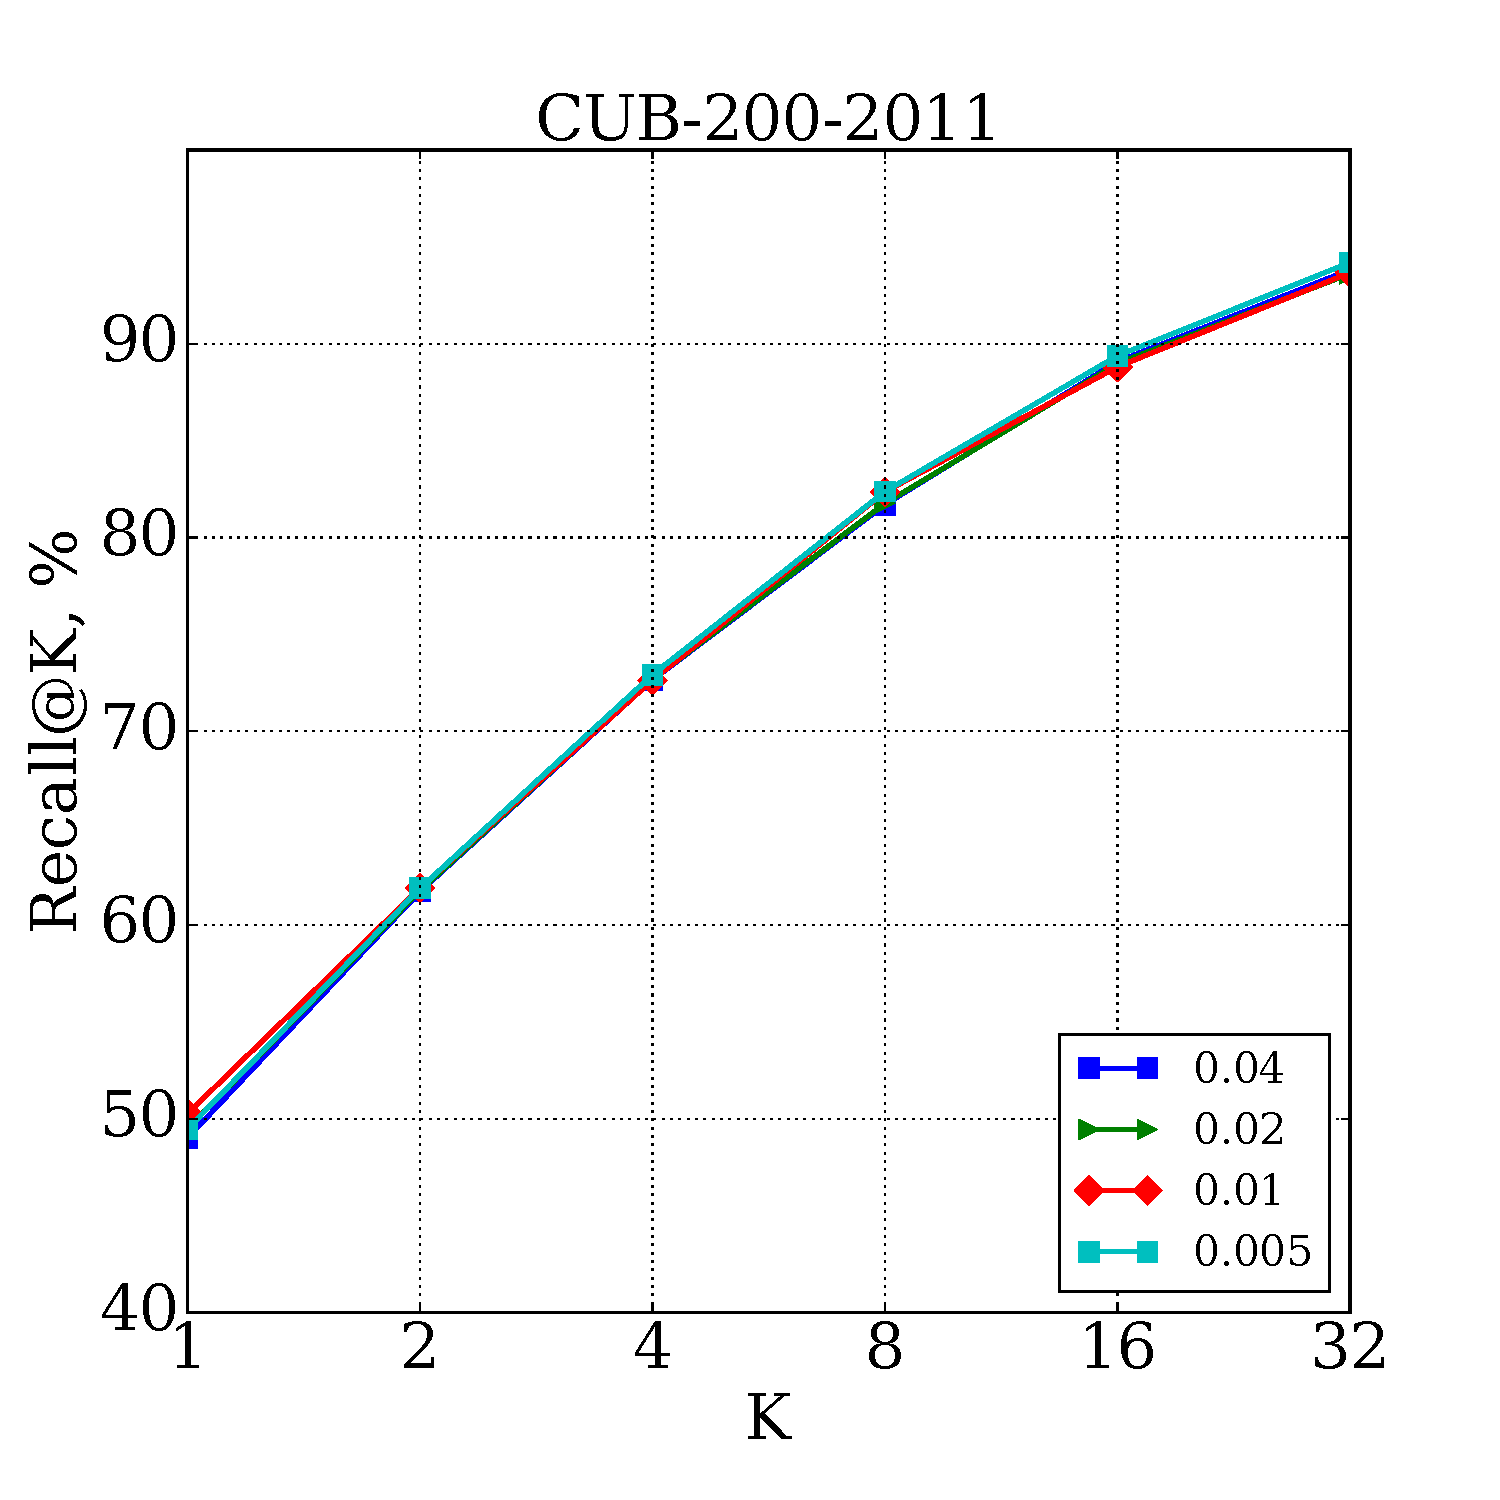
\includegraphics[width=0.7\textwidth]{\histroot/figures/birds_recall_grids.pdf}\\
      (a)\\
    % \begin{subfigure}{0.33\textwidth}
    %   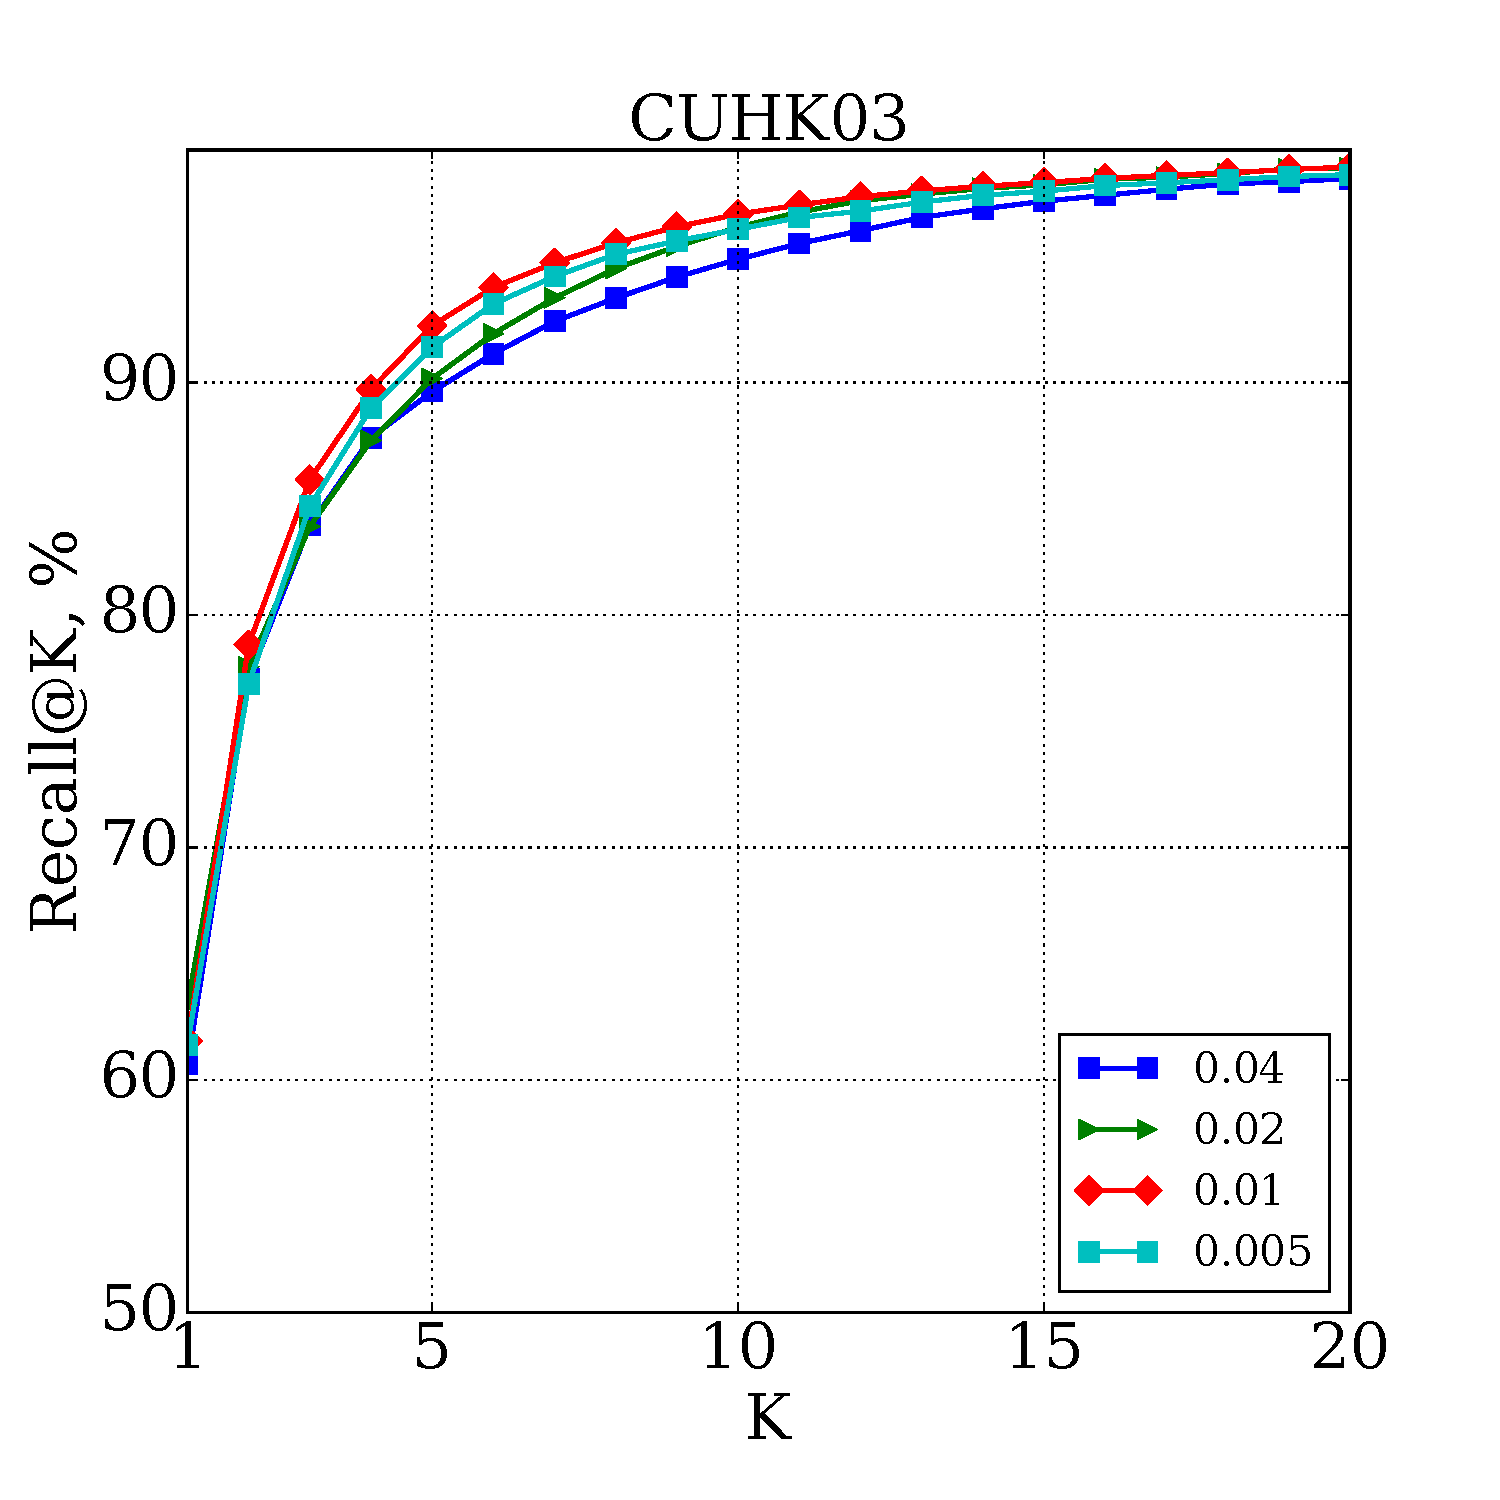
\includegraphics[width=\linewidth]{\histroot/figures/cuhk03_labeled_split1_recall_grids.pdf}
    % \end{subfigure}

        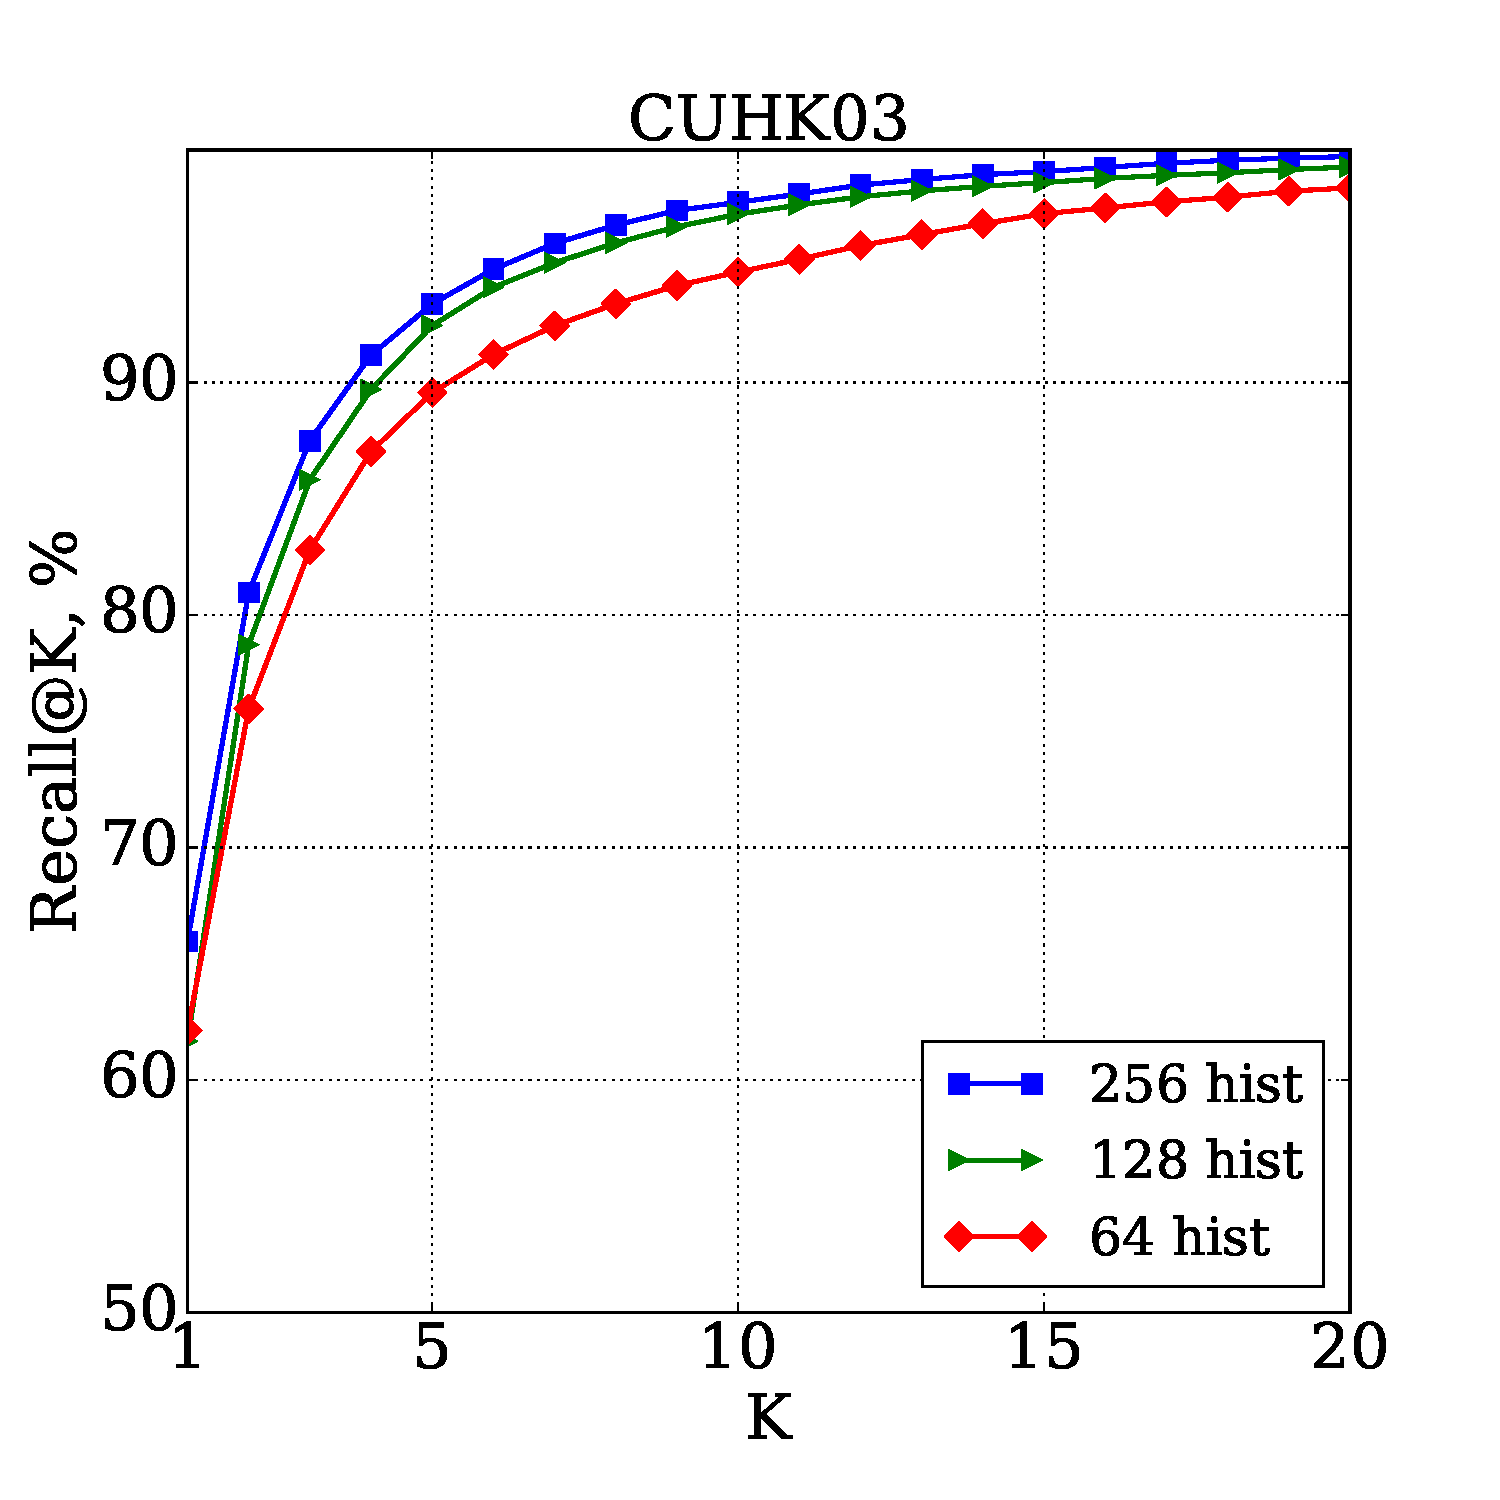
\includegraphics[width=0.7\textwidth]{\histroot/figures/cuhk03_labeled_split1_recall_batch_size.pdf}\\
        (b)\\
\end{tabular}
    \caption{(a) - Recall@K for the CUB-200-2011 dataset for the Histogram loss \eq{loss}. Different curves correspond to variable histogram step $\Delta$, which is the only parameter inherent to our loss.  The curves are very similar for CUB-200-2011. (b) - Recall@K for the CUHK03 labeled dataset for different batch sizes. Results for batch size $256$ is uniformly better than those for smaller values.
    }
    \label{fig:additional}
\end{center}
\end{figure}





\section{Experiments}
In this section we present the results of embedding learning. %for four image datasets: two datasets for person re-identification, one for product image search, and one for fine-grained bird recognition. 
We compare our loss to state-of-the-art pairwise and triplet losses, which have been reported in recent works to give state-of-the-art performance on these datasets.

{\bf Baselines.} \\
In particular, we have evaluated the Binomial Deviance loss \eq{bindev} \citep{Yi14}. While we are aware only of its use in person re-identification approaches, in our experiments it performed very well for product image search and bird recognition significantly outperforming the baseline pairwise (contrastive) loss reported in \citep{Song16}, once its parameters are tuned. %The binomial deviance loss is defined as:

% \begin{equation}
% \label{eq:bindev}
% J_{dev} = \sum_{i,j \in I} w_{i,j} \ln (\exp^{-\alpha (s_{i,j}-\beta) m_{i,j}} +1 ), 
% \end{equation}
% where $I$ is the set of training image indices, and $s_{i,j}$ is the similarity measure between $i$th and $j$th images (i.e.\ $s_{i,j} = cosine(x_{i}, x_{j}$).

% Furthermore,  $m_{i,j}$ and $w_{i, j}$ are the learning supervision and scaling factors respectively:
% \begin{equation}
%     \label{eq:bindev_weights}
%     m_{i, j} = \left\{
% 	\begin{array}{l l}
% 		1,  ${if $(i,j)$ is a positive pair,}$ &\\
% 	   -C,  ${if $(i,j)$ is a negative pair,}$ &
% 	\end{array}\right.
%      w_{i, j}= \left\{
% 	\begin{array}{l l}
% 		\frac {1}{n_1},  ${if $(i,j)$ is a positive pair,}$ &\\
% 		\frac {1}{n_2},  ${if $(i,j)$ is a negative pair,}$ &
% 	\end{array}\right.
% \end{equation}	

% where $n_1$ and $n_2$ are the number of positive and negative pairs in the training set (or mini-batch) correspondingly, $\alpha$ and $\beta$ are hyper-parameters. Parameter $C$ is the negative cost for balancing weights for positive and negative pairs that was introduced in \citep{Yi14}. 
Our experimental results suggest that the quality of the embedding is sensitive to parameter $C$ of the Binomial Deviance loss. Therefore, in the experiments we report results for the two versions of the loss: with $C=10$ that is close to optimal for re-identification datasets, and with $C=25$ that is close to optimal for the product and bird datasets.

We have also computed the results for the Lifted Structured Similarity Softmax (LSSS) loss \eq{lifted} \citep{Song16} on CUB-200-2011 \citep{Wah11} and Online Products \citep{Song16} datasets  and additionally applied it to  re-identification datasets. Lifted Structured Similarity Softmax loss is triplet-based and uses sophisticated triplet sampling strategy that was shown in \citep{Song16} to outperform standard triplet-based loss. 


Additionally, we performed experiments for the triplet loss \citep{SchroffKP15} that uses ``semi-hard negative'' triplet sampling. Such sampling considers only triplets violating the margin, but still having the positive distance smaller than the negative distance.


\begin{figure}
\begin{center}
\begin{tabular}{c}

        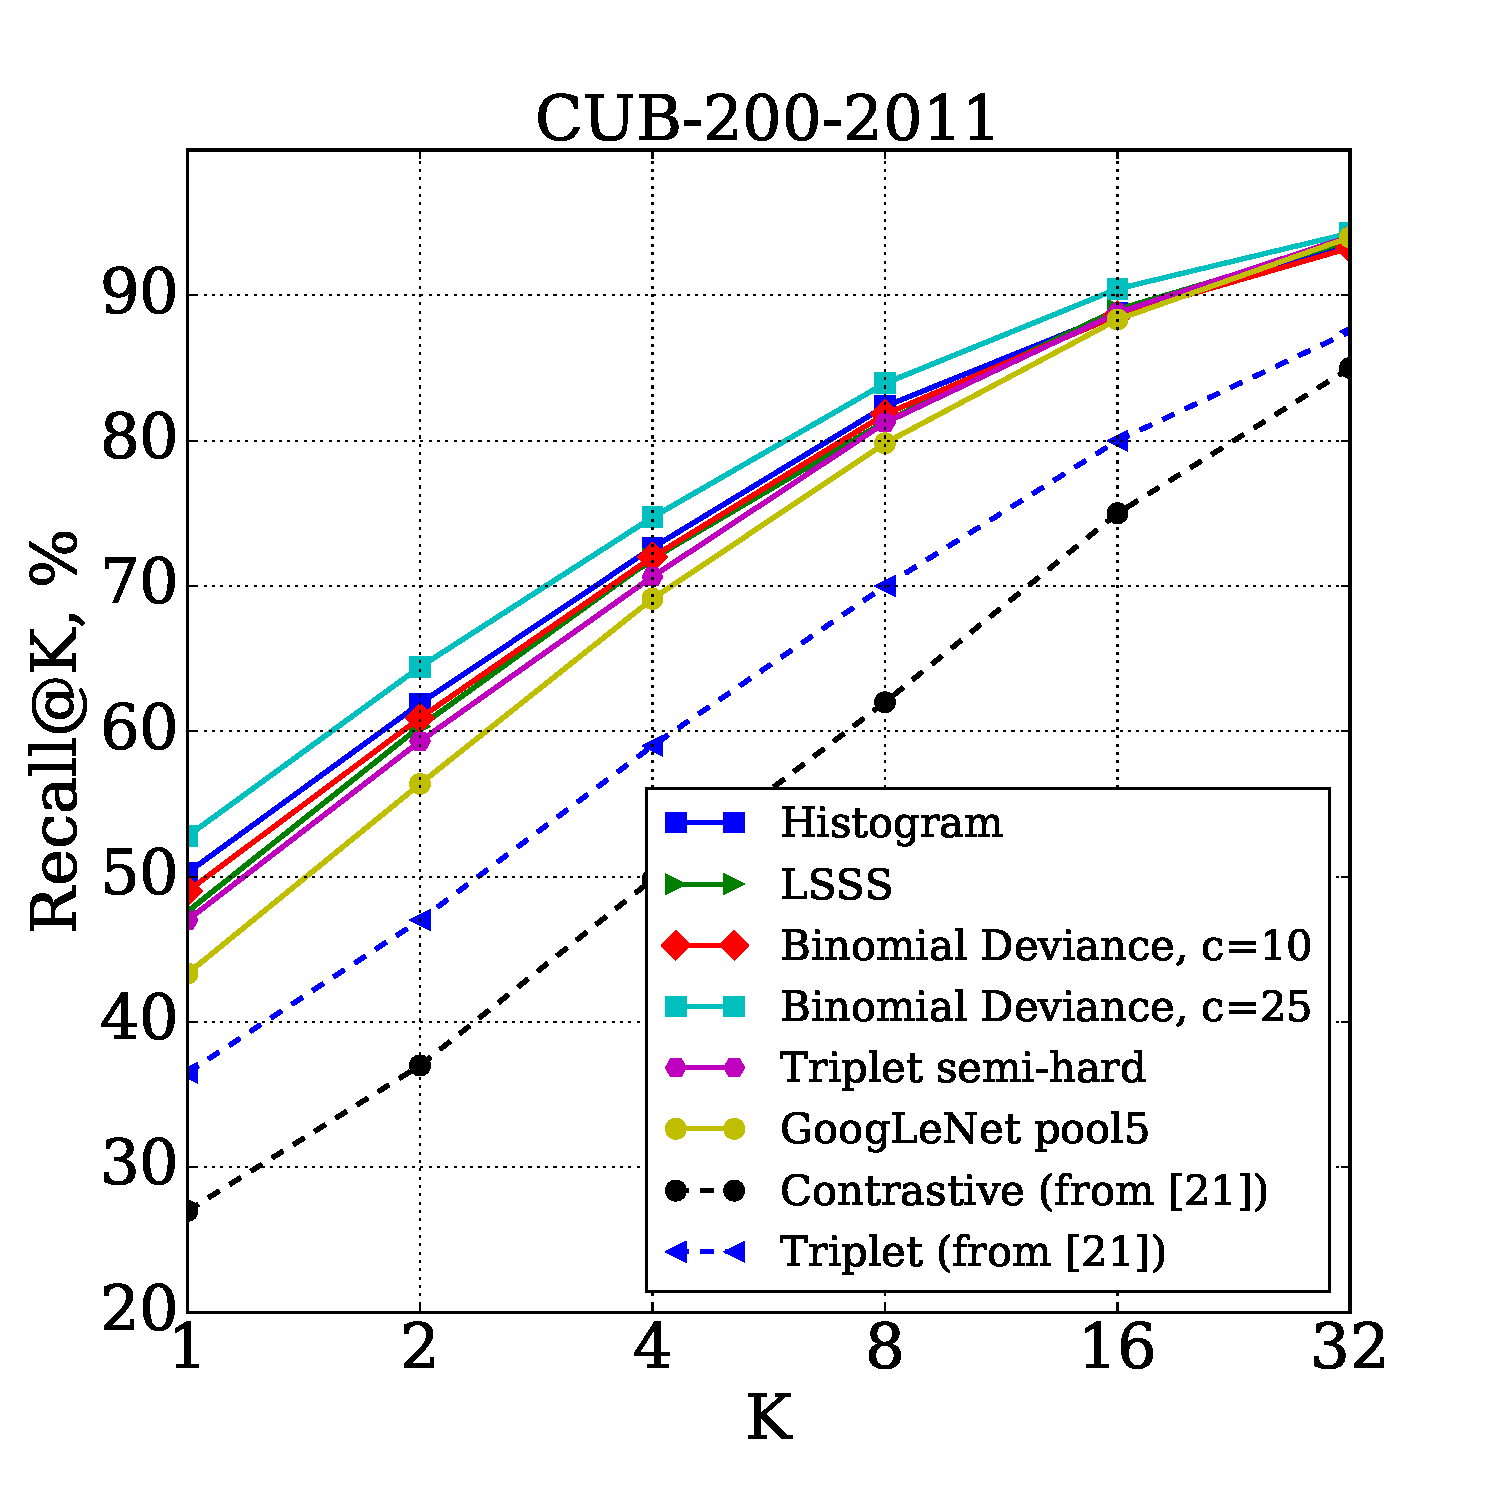
\includegraphics[width=0.7\textwidth]{\histroot/figures/birds_recall.pdf}\\
        (a)\\
    %    \caption{}
    %    \label{fig:birds_recall}


        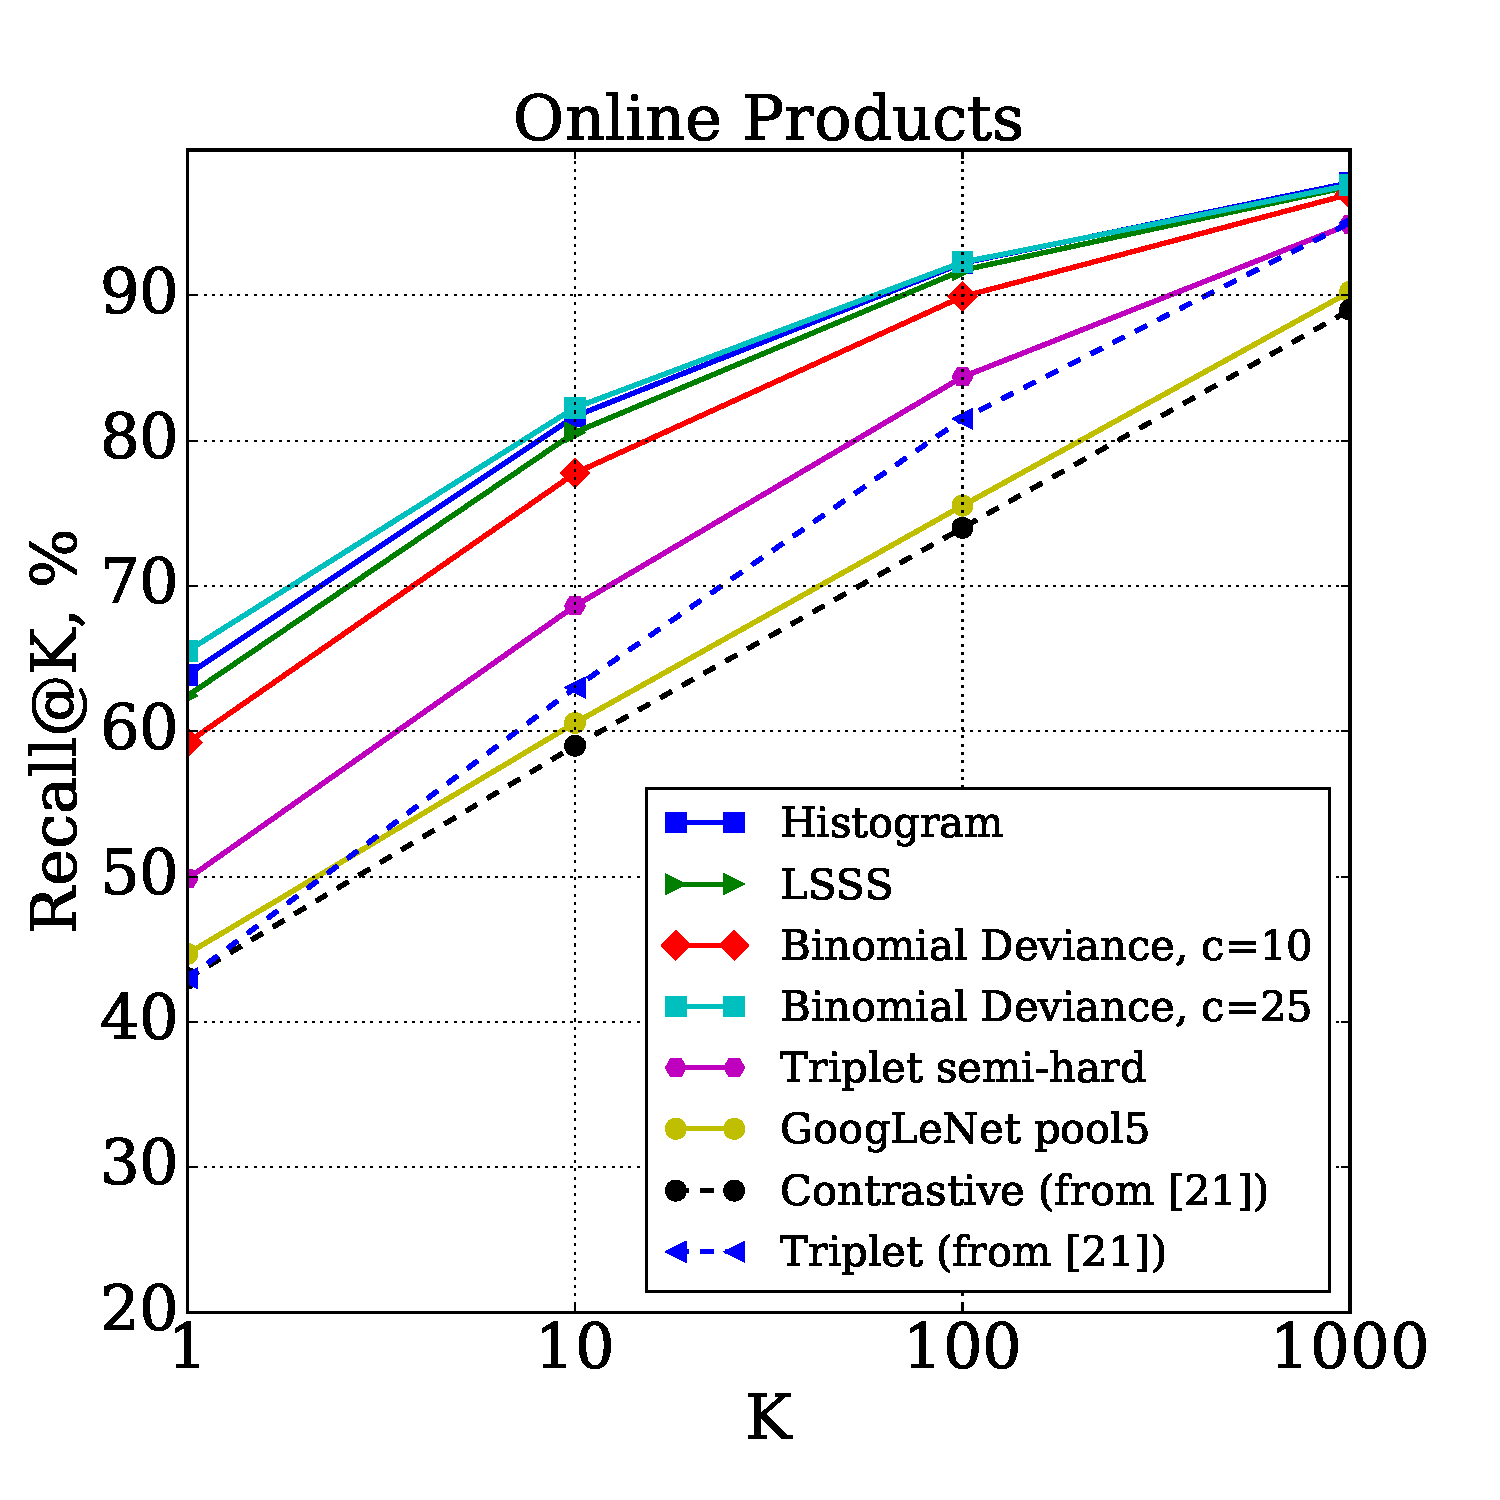
\includegraphics[width=0.7\textwidth]{\histroot/figures/products_recall.pdf}\\
        (b)\\
    %    \caption{}
    %    \label{fig:products_recall}
\end{tabular}
    \caption{Recall@K for (a) - CUB-200-2011 and (b) - Online Products datasets for different methods. Results for the Histogram loss \eq{loss}, Binomial Deviance \eq{bindev}, LSSS \eq{lifted} \citep{Song16} and Triplet \eq{triplet} \citep{SchroffKP15} losses are present. Binomial Deviance loss for $C=25$ outperforms all other methods. The best-performing method is Histogram loss. We also include results for contrastive and triplet losses from \citep{Song16}.
    }
    \label{fig:birds_products}
\end{center}
\end{figure}


%------------- to main into------------
\noindent\textbf{Datasets and evaluation metrics.}\\
We have evaluated the above mentioned loss functions on the four datasets : CUB200-2011 \citep{Wah11}, CUHK03 \citep{Li14}, Market-1501 \citep{Zheng15} and Online Products \citep{Song16}. All these datasets have been used for evaluating methods of solving embedding learning tasks. 
Specifically, the Online Products dataset introduced in \citep{Song16} along with CUB200-2011 was used for training a deep image retrieval model \citep{Song16}. CUHK03 and  Market-1501 are the largest datasets for person re-identification available at the moment. 

Commonly, for the retrieval tasks training and testing are done using disjoint sets of classes. For many datasets, including above mentioned ones, the standard splits for evaluation are provided.
The CUB-200-2011 dataset includes 11,788 images of 200 classes corresponding to different birds species. As in \citep{Song16} we use the first 100 classes for training
(5,864 images) and the remaining classes for testing
(5,924 images).
% %Online products
The Online Products dataset includes 120,053 images of 22,634 classes. Classes correspond to a number of online products from eBay.com. There are approximately 5.3 images for each product. We used the standard split from \citep{Song16}: 11,318 classes (59,551 images)  are used for training and 11,316 classes (60,502 images) are used for testing.
The images from the CUB-200-2011 and the Online Products datasets are resized to 256 by 256, keeping the original aspect ratio (padding is done when needed). The Recall@K metric is calculated for the set of queries consisting of all the images in the test set.

% %CUHK03
% The CUHK03 dataset is commonly used for the person re-identification task. It includes 13,164 images of 1,360 pedestrians captured from 3 pairs of cameras. Each identity is observed by two cameras and has 4.8 images in each camera on average.  Following most of the previous works we use the ``CUHK03-labeled'' version of the dataset with manually-annotated bounding boxes. According to the CUHK03 evaluation protocol, 1,360 identities are split into 1,160 identities for training, 100 for validation and 100 for testing. We use the first split from the CUHK03 standard split set which is provided with the dataset. 
% %MVS
% % The Multi-view Stereo Correspondence dataset (MVS) contains over 1.5M grayscale image patches of size 64$\times$64. The patches are sampled around more than 500K 3D points in different views. There are three patches subsets in MVS: patches are sampled from 3D reconstructions of the Statue of Liberty (New York), Notre Dame (Paris) and Half Dome (Yosemite). For each of the three subsets a number of patches pairs with their ground truth labels are provided for evaluation. The common protocol used for MVS is training on the one subset and testing on the two other subsets.
% %The second re-identification dataset we use is Market-1501, introduced in \citep{Zheng15}.
% %(See figure \ref{fig:datasets_market} for sample images). 
% The Market-1501 dataset includes 32,643 images of 1,501 pedestrians, each pedestrian is captured by several cameras (from two to six). The dataset is divided randomly  into the test set of 750 identities and the train set of 751 identities. %We use 51 identities from the train set for validation. In the test set there are several query images for each identity: one image from each camera is selected for each pedestrian. When testing, all the images of the query person captured from the same camera as the query image are excluded from the gallery.% Manually drawn bounding boxes are used for query images, and automatically detected ones for training images as well as for the gallery images in the test set. %Market-1501 also contains ''distractor'' images as a part of the gallery set. These images correspond to false detections and are ''negatives'' to all the queries, which makes evaluation on the dataset even more challenging. 
% %the test data

%\footnote{Recall@K is the probability of getting the right match among first K gallery candidates sorted by similarity.}
Following \citep{Song16,Yi14,Zheng15}, we report Recall@K metric for all the datasets.  For CUB-200-2011 and Online products,  every test image is used as the query in turn and remaining images are used as the gallery correspondingly. In contrast, for CUHK03 \textit{single-shot} results are reported. This means that one image for each identity from the test set is chosen randomly in each of its two camera views. Recall@K values for 100 random query-gallery sets are averaged to compute the final result for a given split. For the Market-1501 dataset, we use the \textit{multi-shot} protocol (as is done in most other works), as there are many images of the same person in the gallery set.
%----------------------------------
%\begin{wrapfigure}
% \begin{figure}
% \centering
%   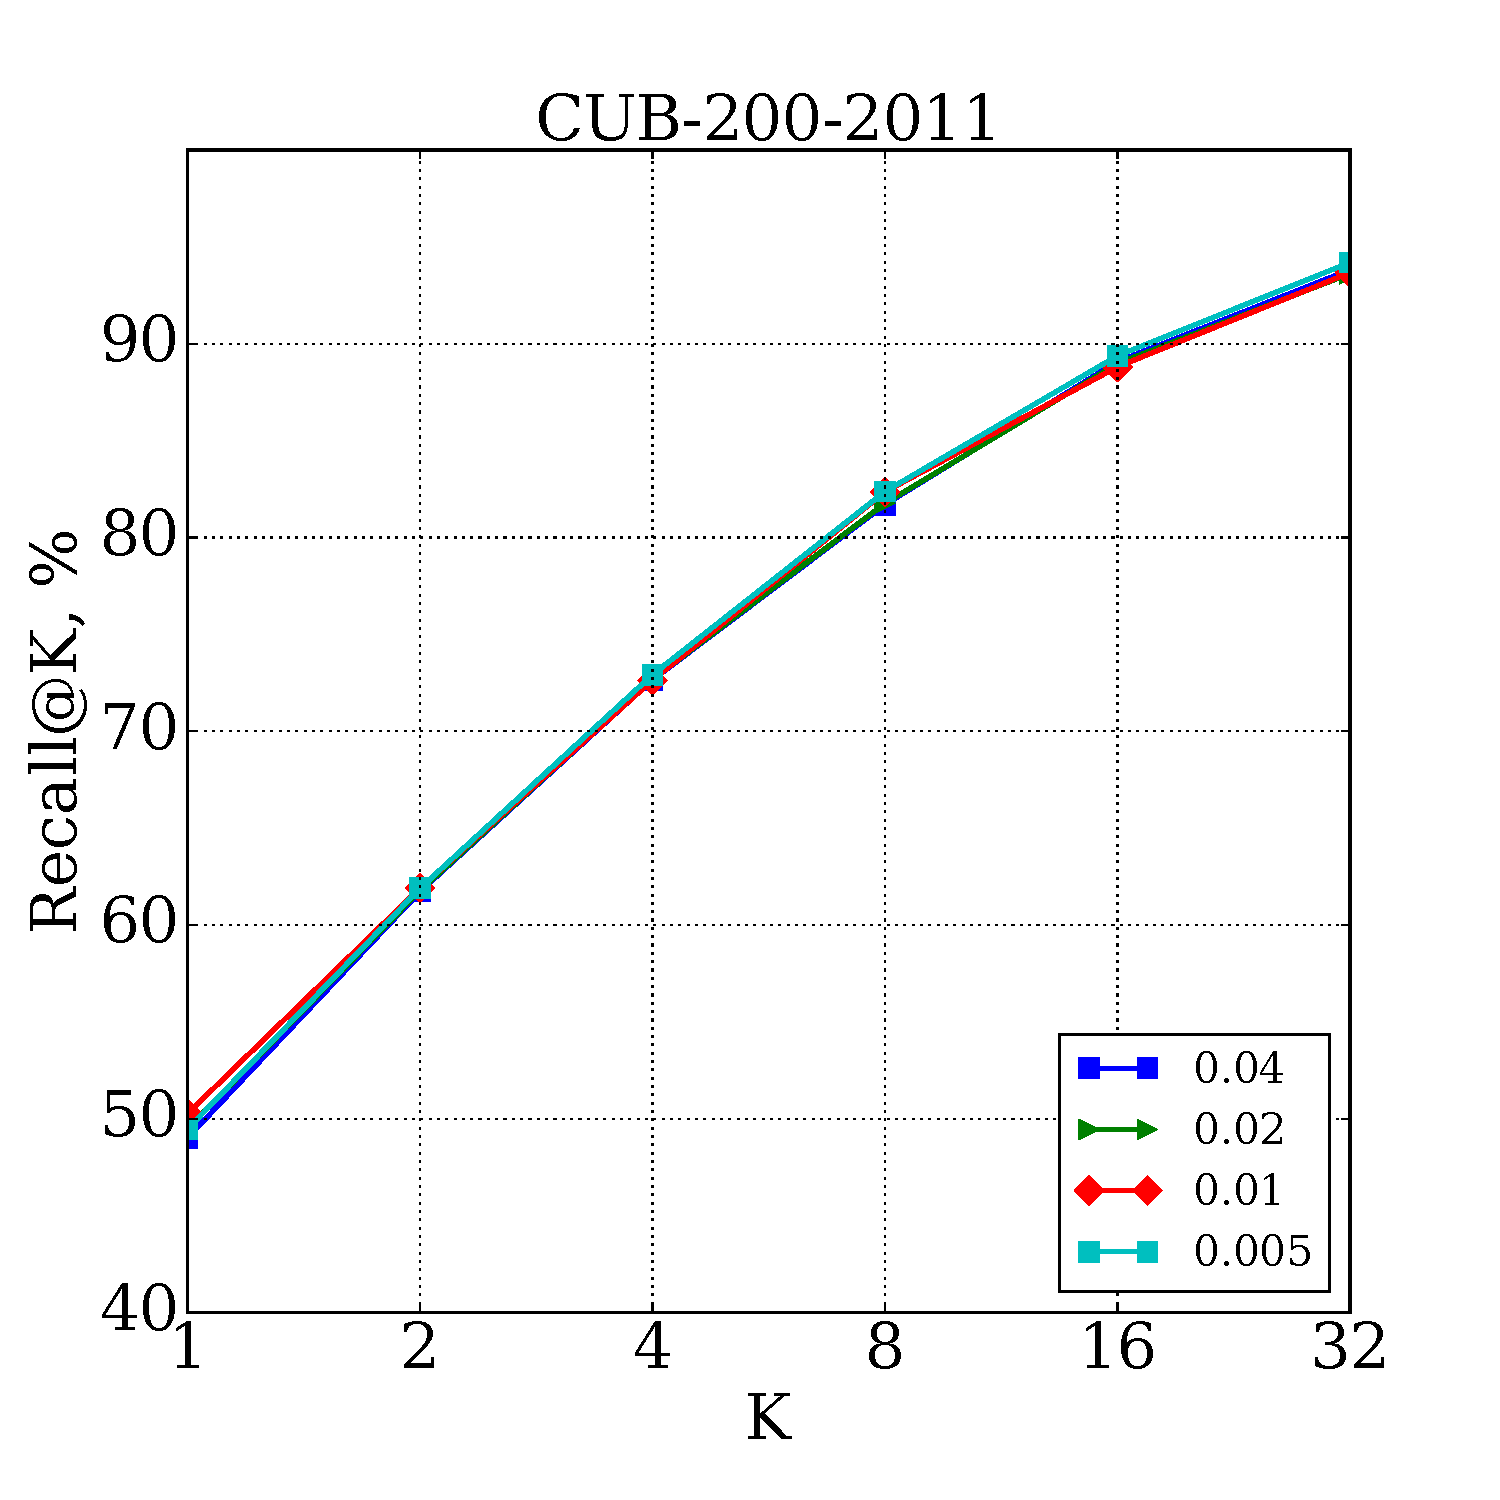
\includegraphics[width=0.4\linewidth]{\histroot/figures/birds_recall_grids.pdf}
%          \caption{Recall@K for the CUB-200-2011 dataset for the Histogram loss \eq{loss}. Different curves correspond to variable histogram step $\Delta$, which is the only parameter inherent to our loss.  The curves are very similar despite an order of magnitude variation.}
%          \label{fig:birds_recall_grids}
%   % \end{left}
 
% \end{figure}

\begin{figure}
\begin{center}
\begin{tabular}{c}
 
        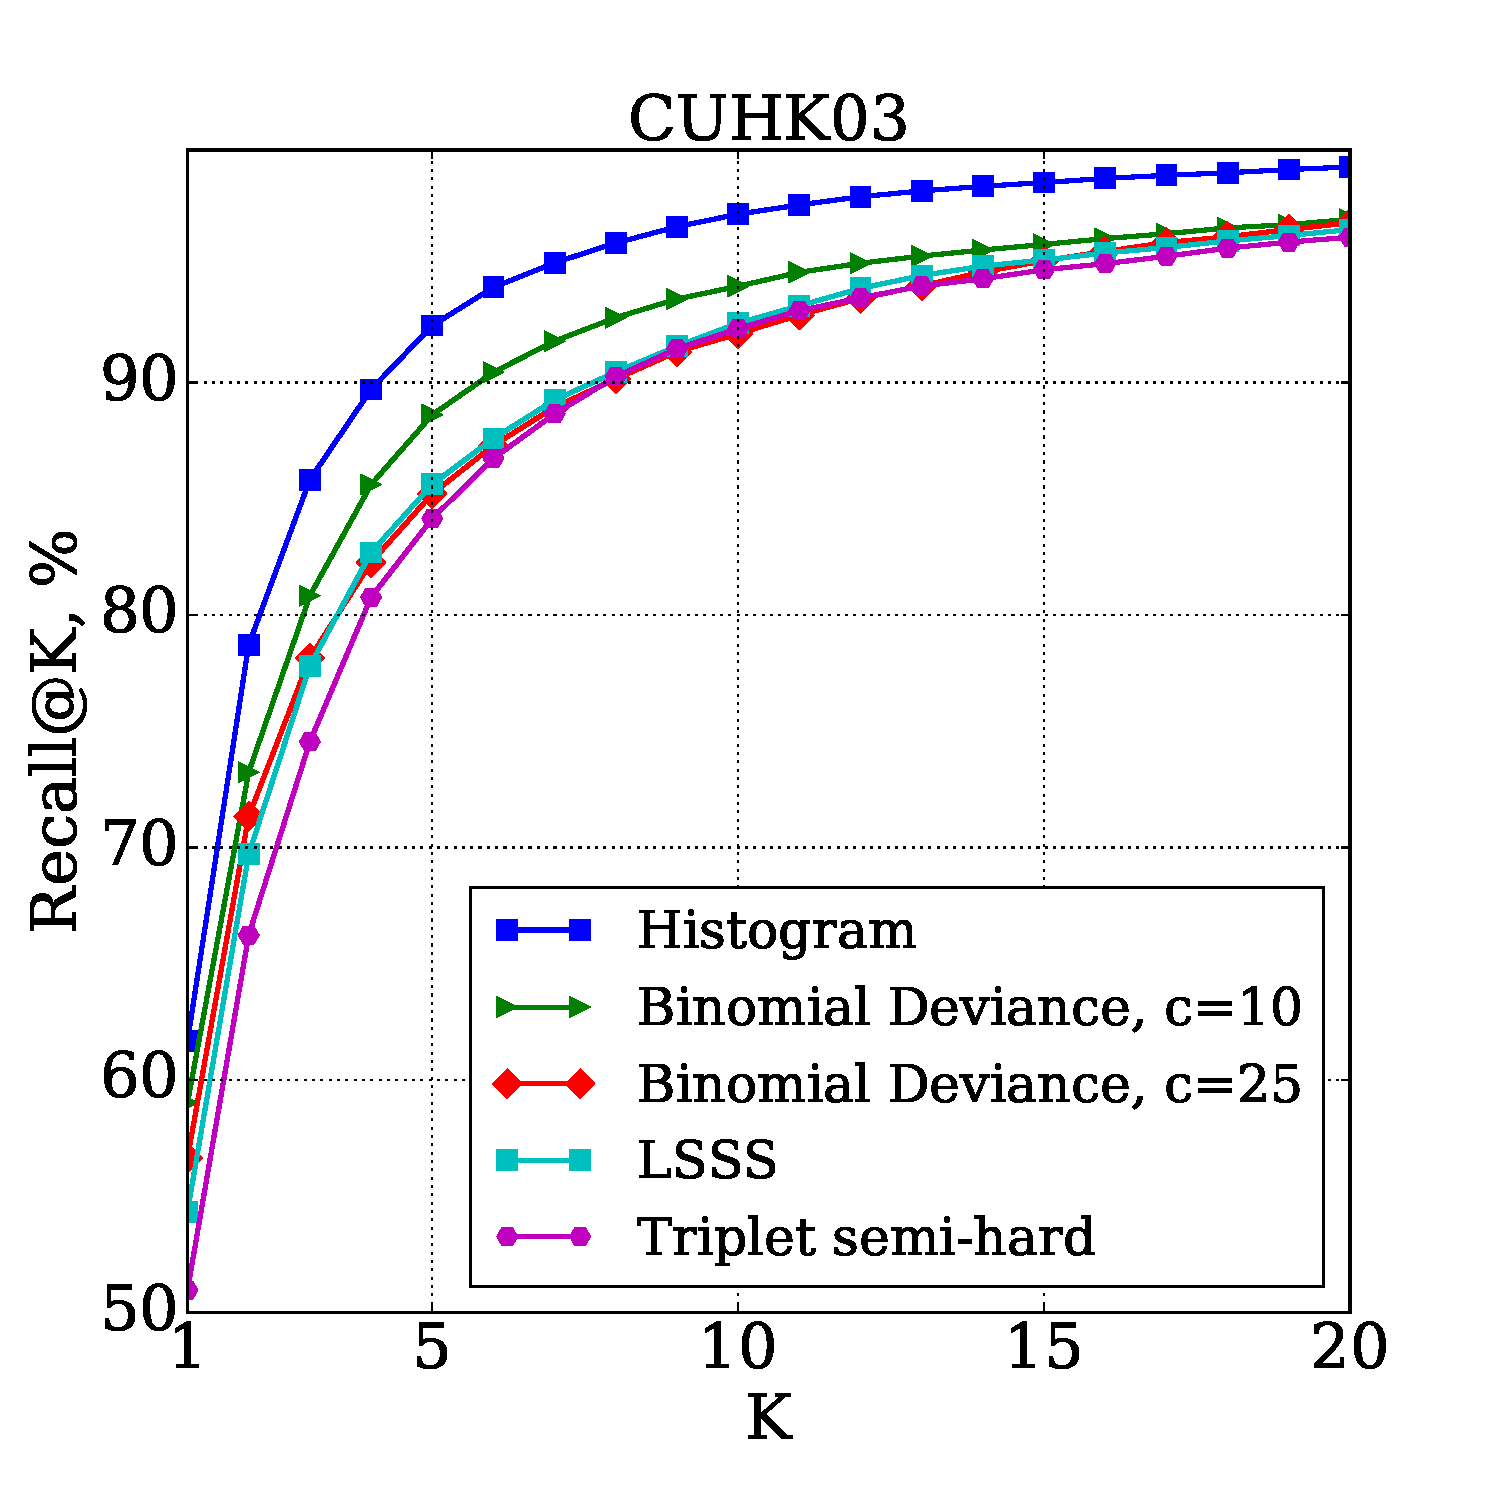
\includegraphics[width=0.7\textwidth]{\histroot/figures/cuhk03_labeled_split1_recall.pdf} \\
        (a) \\
      %  \caption{}
      %  \label{fig:cuhk03_labeled_split1_recall}
  
    
        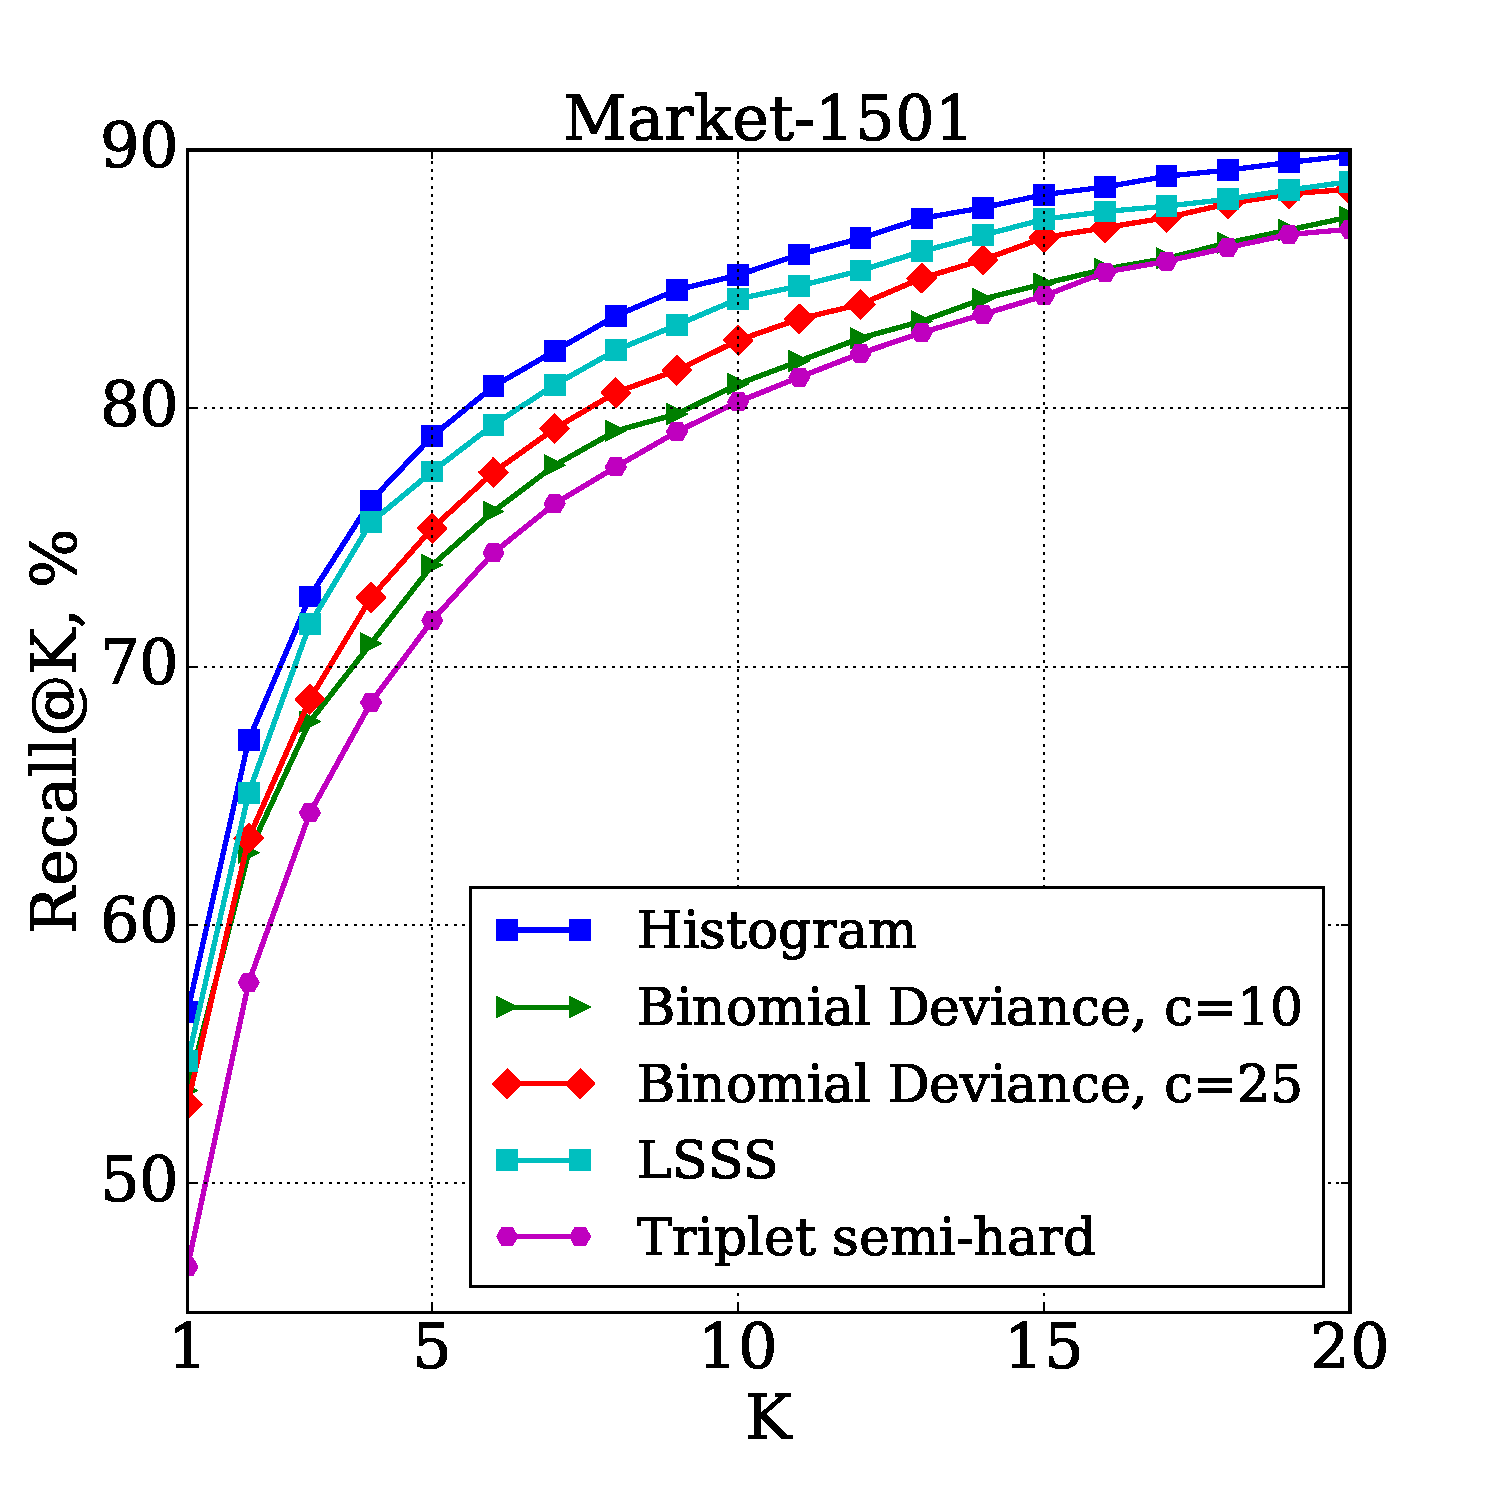
\includegraphics[width=0.7\textwidth]{\histroot/figures/market_recall.pdf}\\
        (b) \\
      %  \caption{}
      %  \label{fig:market_recall}

\end{tabular}
    \caption{Recall@K for (a) - CUHK03 and (b) -  Market-1501 datasets. The Histogram loss \eq{loss} outperforms Binomial Deviance, LSSS and Triplet losses. }
    \label{fig:reid_recall}   
\end{center}
\end{figure}

\noindent\textbf{Architectures used.}\\
For training on the CUB-200-2011 and the Online Products datasets we used the same architecture as in \citep{Song16}, which conincides with the GoogleNet architecture \citep{szegedy2015going} up to the `pool5' and the inner product layers, while the last layer is used to compute the embedding vectors. The GoogleNet part is pretrained on ImageNet ILSVRC \citep{ILSVRC15} and the last layer is trained from scratch. As in \citep{Song16}, all GoogLeNet layers are fine-tuned with the learning rate that is ten times less than the learning rate of the last layer. We set the embedding size to 512 for all the experiments with this architecture. We reproduced the results for the LSSS loss \eq{lifted} \citep{Song16} for these two datasets. For the architectures that use the Binomial Deviance loss, Histogram loss and Triplet loss the iteration number and the parameters value (for the former) are chosen using the validation set.    


For training on CUHK03 and Market-1501 we used the Deep Metric Learning (DML) architecture introduced in \citep{Yi14}. It has been described in \sect{intro_architectures}. 

\begin{table}%{0.6\textwidth}
\begin{center}
\caption{Final results for CUHK03-labeled and Market-1501. For CUHK03-labeled results for 5 random splits were averaged. Batch of size 256 was used for both experiments.}\label{tab:reid}
\begin{tabular}{cccccc}\\\toprule  
Dataset      & r = 1     &  r = 5     & r = 10    & r = 15     & r = 20 \\\midrule
 CUHK03      & 65.77 & 92.85 & 97.62 &  98.94 & 99.43\\  %\midrule
 Market-1501 & 59.47 & 80.73 & 86.94 &  89.28 & 91.09 \\  \bottomrule
\end{tabular}
\end{center}
\end{table} 

\noindent\textbf{Implementation details.}\\
For all the experiments with loss functions \eq{loss} and \eq{bindev} we used quadratic number of pairs in each batch (all the pairs that can be sampled from batch). For triplet loss ``semi-hard'' triplets chosen from all the possible triplets in the batch are used. For comparison with other methods the batch size was set to $128$. We sample batches randomly in such a way that there are several images for each  sampled class in the batch. We iterate over all the classes and all the images corresponding to the classes, sampling images in turn. The sequences of the classes and of the corresponding images are shuffled for every new epoch. CUB-200-2011 and Market-1501 include more than ten images per class on average, so we limit the number of images of the same class in the batch to ten for the experiments on these datasets. We used ADAM \citep{Kingma14} for stochastic optimization in all of the experiments. For all losses the learning rate is set to $1e-4$ for all the experiments except ones on the CUB-200-2011 datasets, for which we have found the learning rate of $1e-5$ more effective. 
For the re-identification datasets the learning rate was decreased by 10 after the 100K iterations, for the other experiments learning rate was fixed. The iterations number for each method was chosen using the validation set.

\noindent\textbf{Results.}\\
The Recall@K values for the experiments on CUB-200-2011, Online Products, CUHK03 and Market-1501 are shown in \fig{birds_products} and \fig{reid_recall}. The Binomial Deviance loss \eq{bindev} gives the best results for CUB-200-2011 and Online Products with the $C$ parameter set to $25$. We previously checked several values of $C$ on the CUB-200-2011 dataset and found the value $C=25$ to be the optimal one. We also observed that with smaller values of $C$ the results are significantly worse than those presented in the \fig{birds_products}a (for $C$ equal to $2$ the best Recall@1 is 43.50\%). For CUHK03 the situation is reverse: the Histogram loss gives the boost of 2.64\% over the Binomial Deviance loss with $C=10$ (which we found to be optimal for this dataset). The results are shown in the figure \fig{reid_recall}a. Embedding distributions of the positive and negative pairs from CUHK03 test set for different methods are shown in Figure  \ref{fig:distr}.
For the Market-1501 dataset our method also outperforms the Binomial Deviance loss for both values of $C$. In contrast to the experiments with CUHK03, the Binomial Deviance loss appeared to perform better with $C$ set to $25$ than to $10$ for Market-1501. We have also investigated how the size of the histogram bin affects the model performance for the Histogram loss. As shown in the \fig{additional}a, the results for CUB-200-2011 remain stable for the sizes equal to 0.005, 0.01, 0.02 and 0.04 (these values correspond to 400, 200, 100 and 50 bins in the histograms). In our method,  distributions of similarities of training data are estimated by distributions of similarities within mini-batches. Therefore we also show results for the Histogram loss for various batch size values (\fig{additional}b). The larger batches are more preferable: for CUHK03, Recall@K for batch size equal to $256$ is uniformly better than Recall@K for $128$ and $64$. We also observed similar behaviour for Market-1501. Additionally, we present our final results (batch size set to 256) for CUHK03 and Market-1501 in \tab{reid}. For CUHK03, Rekall@K values for 5 random splits were averaged. To the best of our knowledge, these results corresponded to state-of-the-art on CUHK03 and Market-1501 at the moment of submission. 
To summarize the results of the comparison: the new (Histogram) loss gives the best results on the two person re-identification problems. For CUB-200-2011 and Online Products it came very close to the best loss (Binomial Deviance with $C=25$). Interestingly, the histogram loss uniformly outperformed the triplet-based LSSS loss \eq{lifted} \citep{Song16} in our experiments including two datasets from \citep{Song16}. Importantly, the new loss does not require to tune parameters associated with it (though we have found learning with our loss to be sensitive to the learning rate).








% \begin{wraptable}{r}{5.5cm}
% \caption{Final results for CUHK03-labeled and Market-1501. For CUHK03-labeled results for 5 random splits were used. Batch of size 256 was user for both experiments.}\label{reid}
% \begin{tabular}{\linewidth}{c|ccccc}
%     \hline
%  %  & \multicolumn{2}{c}{CUHK03} & \multicolumn{2}{c}{Market}\\
   
%     % \hline
%     % rank & 128 & 256 & 128 & 256  \\
%     % 1    & 64.15 & 65.77 & 56.62 & 59.47 \\
%     % 5    & 91.66 & 92.85 & 78.92 & 80.73 \\
%     % 10   & 96.97 & 97.62 & 85.15 & 86.94 \\
%     % 15   & 98.58 & 98.94 & 88.27 & 89.28 \\
%     % 20   & 99.26 & 99.43 & 89.79 & 91.09 \\
%     % \hline

%     Dataset     & \multicolumn{5}{c}{rank} \\
%                 & 1     & 5     & 10    & 15     & 20 \\ 
%     CUHK03      & 65.77 & 92.85 & 97.62 &  98.94 & 99.43 \\
%     Market-1501 & 59.47 & 80.73 & 86.94 &  89.28 & 91.09 \\
% \end{tabular}    
% \end{wraptable} 


\begin{figure}

\begin{center}
\begin{tabular}{c}
  
        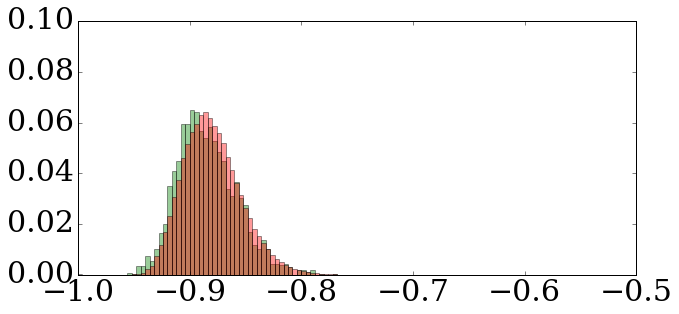
\includegraphics[width=0.7\textwidth]{\histroot/figures/initial_distr_cuhk03.png} \\
        (a) \\
      %  \caption{}
       % \label{fig:initial}
   
  
        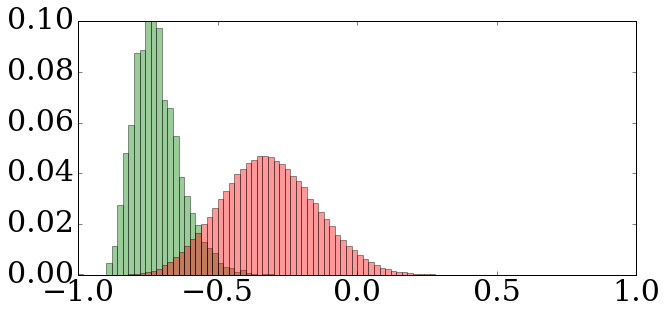
\includegraphics[width=0.7\textwidth]{\histroot/figures/np.png} \\
        (b) \\
     %   \caption{}
     %   \label{fig:np}
  
 
        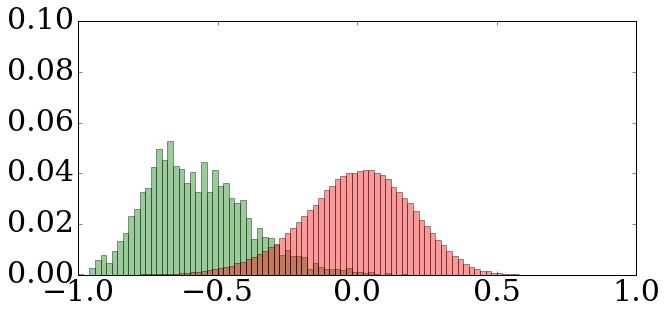
\includegraphics[width=0.7\textwidth]{\histroot/figures/bindev10.png} \\
        (c) \\
    %    \caption{}
  %      \label{fig:bindev10}
    
  %  \begin{subfigure}{\textwidth}
        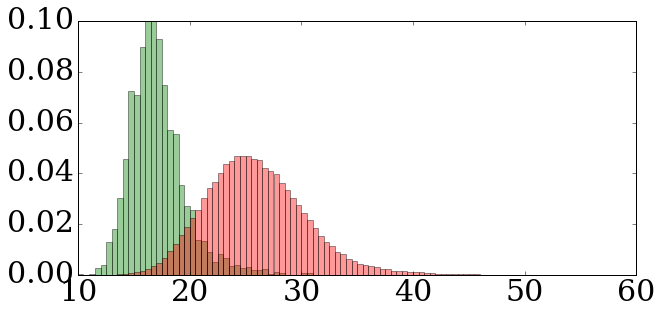
\includegraphics[width=0.7\textwidth]{\histroot/figures/lifted.png} \\
        (d) \\
  %      \caption{}
   %     \label{fig:lifted}
   %     \end{subfigure}   
 \end{tabular}
\end{center}      
    
    \caption{Histograms for positive and negative distance distributions on the CUHK03 test set for: (a) Initial state: randomly initialized net, (b) Network training with the Histogram loss, (c) same for the Binomial Deviance loss, (d) same for the LSSS loss. Red is for negative pairs, green is for positive pairs. Negative cosine distance measure is used for Histogram and Binomial Deviance losses, Euclidean distance is used for the LSSS loss. Initially the two distributions are highly overlapped. For the Histogram loss the distribution overlap is less than for the LSSS. }
    \label{fig:distr}    
    

\end{figure}



%-------------------------------------------------------------------------
\section{Conclusion}
In this chapter we have suggested a new loss function for learning deep embeddings, called the Histogram loss. Like most previous losses, it is based on the idea of making the distributions of the similarities of the positive and negative pairs less overlapping. Unlike other losses used for deep embeddings, the new loss comes with virtually no parameters that need to be tuned. It also incorporates information across a large number of quadruplets formed from training samples in the mini-batch and implicitly takes into account all of such quadruplets. We have demonstrated the competitive results of the new loss on a number of datasets. In particular, the Histogram loss outperformed other losses for the person re-identification problem on CUHK03 and Market-1501 datasets. The code for Caffe~\citep{jia2014caffe} is available at: \url{https://github.com/madkn/HistogramLoss}.



\textbf{Acknowledgement:} This research is supported by the Russian Ministry of Science and Education grant RFMEFI57914X0071.

%-------------------------------------------------------------------------

\newpage 



\chapter{Multi-region Bilinear Convolutional Neural Networks for Person Re-Identification}

\label{chapt:bilinear}

\section{Motivation}
%: relation to fine-grained recognition and Bilinear CNNs
%TODO relocate images (false positive-left, )
\begin{figure*}[t]%{R}{0.5\textwidth}
\centering

\begin{tabular}{c c}

    False positives & False negatives \\
    \begin{tabular}{c c }
    % 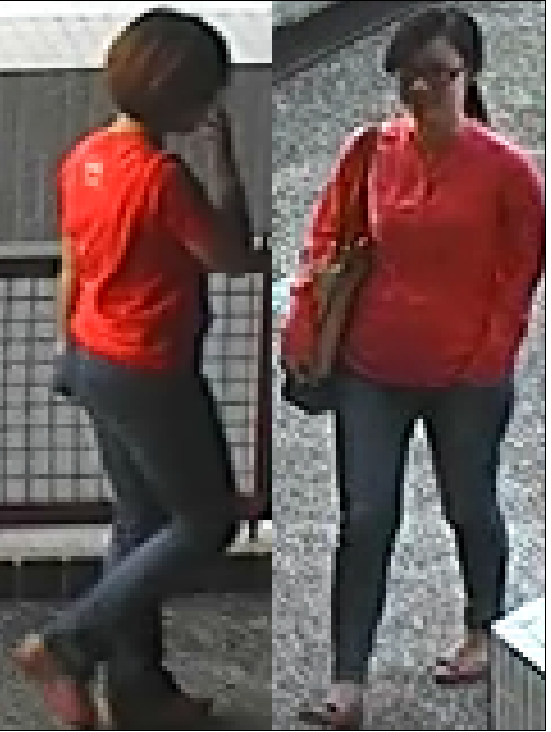
\includegraphics[ height=3.5cm, width=2.5cm]{\bilinearroot/figures/pedestrians_pairs/false_pos1.png}&
    % 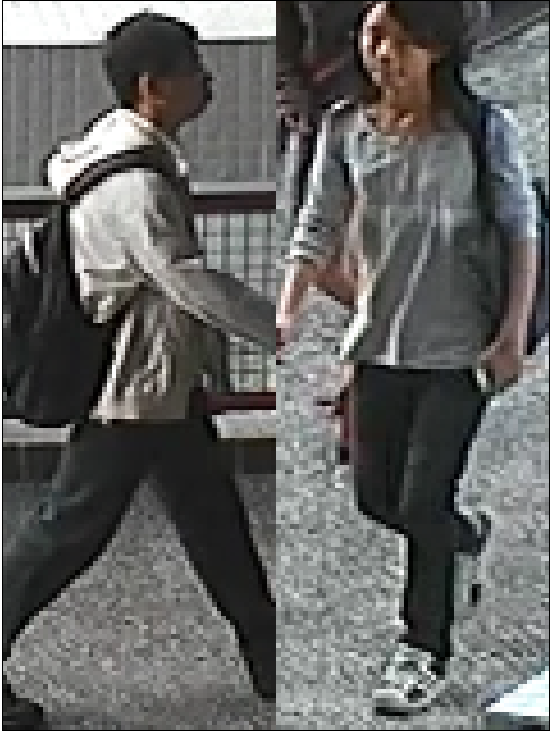
\includegraphics[ height=3.5cm, width=2.5cm]{\bilinearroot/figures/pedestrians_pairs/false_pos2.png}\\
    % 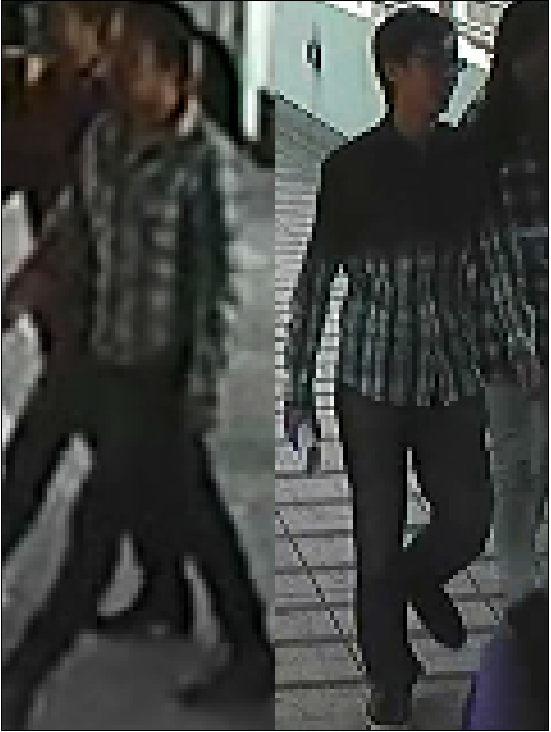
\includegraphics[ height=3.5cm, width=2.5cm]{\bilinearroot/figures/pedestrians_pairs/false_pos3.png}&
    % 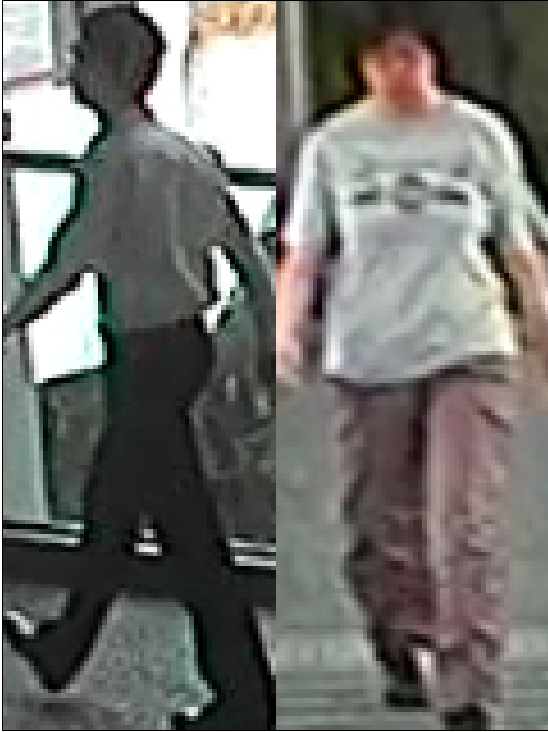
\includegraphics[ height=3.5cm, width=2.5cm]{\bilinearroot/figures/pedestrians_pairs/false_pos4.png}
    
    
    \end{tabular} &
    
    
    \begin{tabular}{c c }

    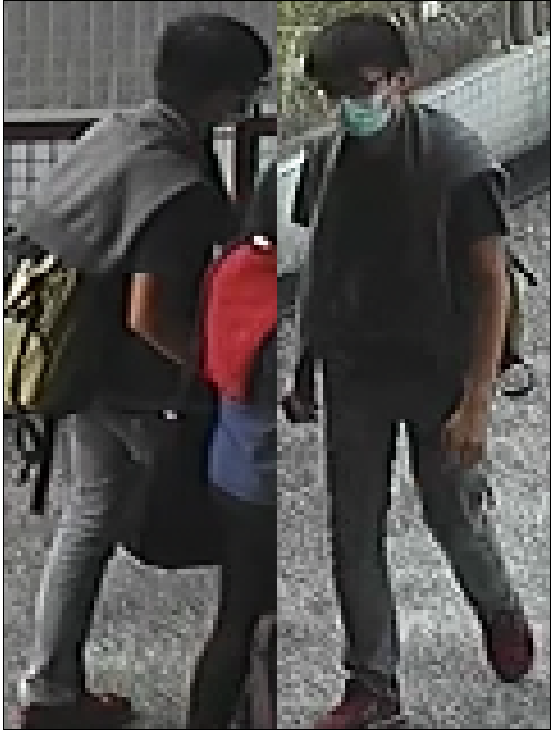
\includegraphics[ height=3.5cm, width=2.5cm]{\bilinearroot/figures/pedestrians_pairs/false_neg1.png}&
    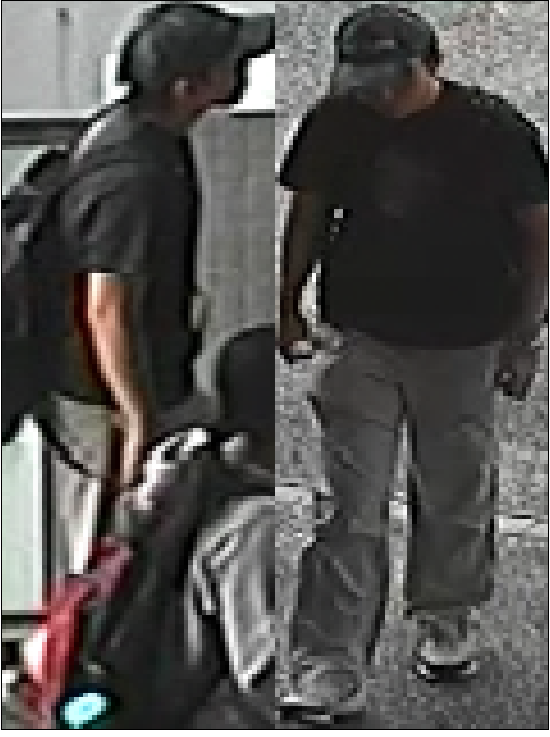
\includegraphics[ height=3.5cm, width=2.5cm]{\bilinearroot/figures/pedestrians_pairs/false_neg2.png}\\
    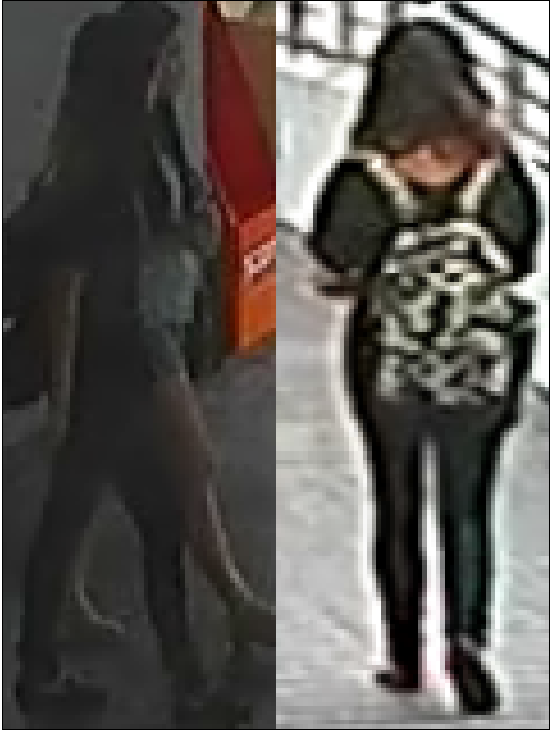
\includegraphics[ height=3.5cm, width=2.5cm]{\bilinearroot/figures/pedestrians_pairs/false_neg3.png}&
    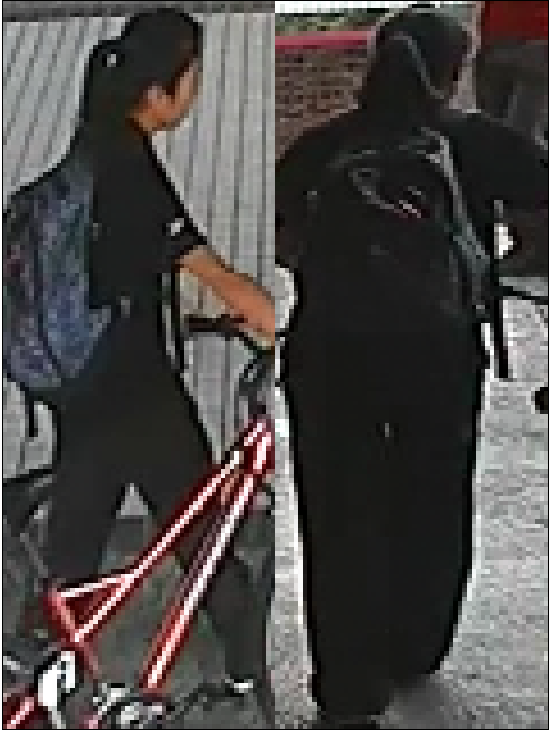
\includegraphics[ height=3.5cm, width=2.5cm]{\bilinearroot/figures/pedestrians_pairs/false_neg4.png}
    
    
    \end{tabular}
    \\

    
    \begin{tabular}{c }
    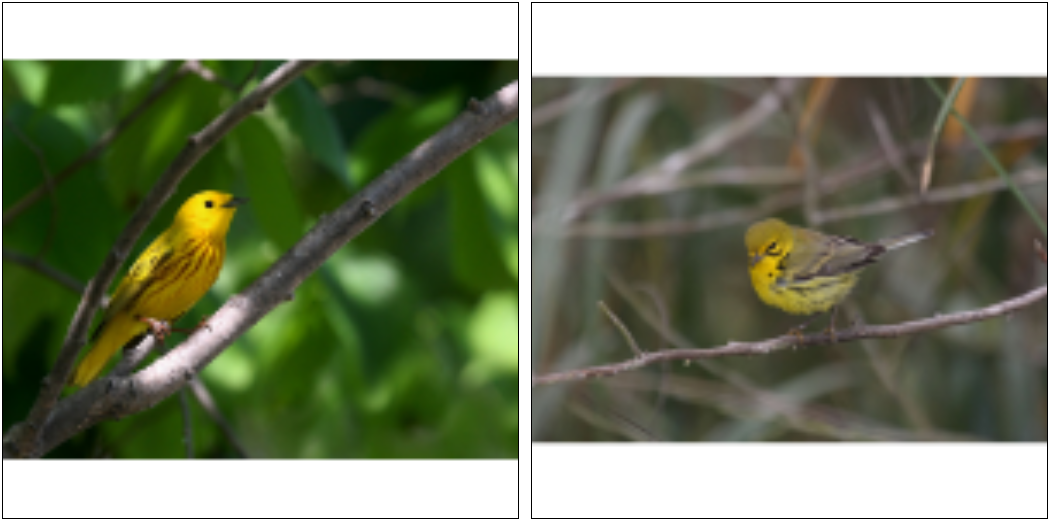
\includegraphics[ height=3cm, width=5.5cm]{\bilinearroot/figures/birds/birds_false_pos1.png}\\
    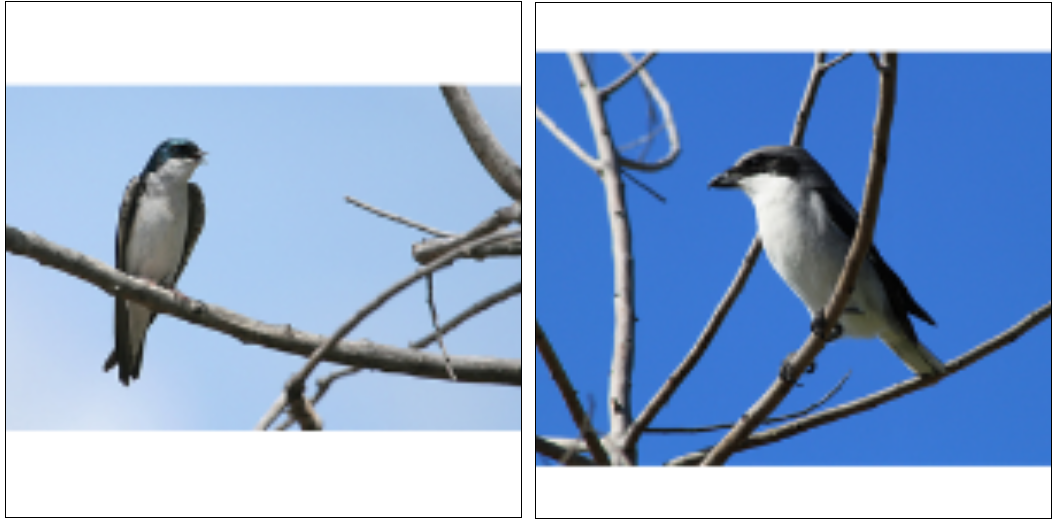
\includegraphics[ height=3cm, width=5.2cm]{\bilinearroot/figures/birds/birds_false_pos2.png}
    
    \end{tabular} &
    \begin{tabular}{c }

    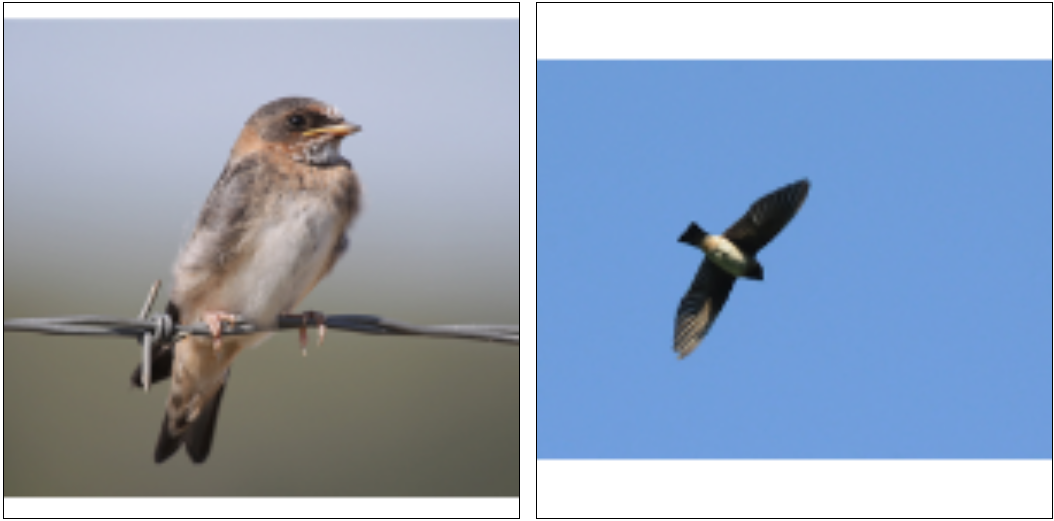
\includegraphics[ height=3cm, width=5.5cm]{\bilinearroot/figures/birds/birds_false_neg1.png}\\
    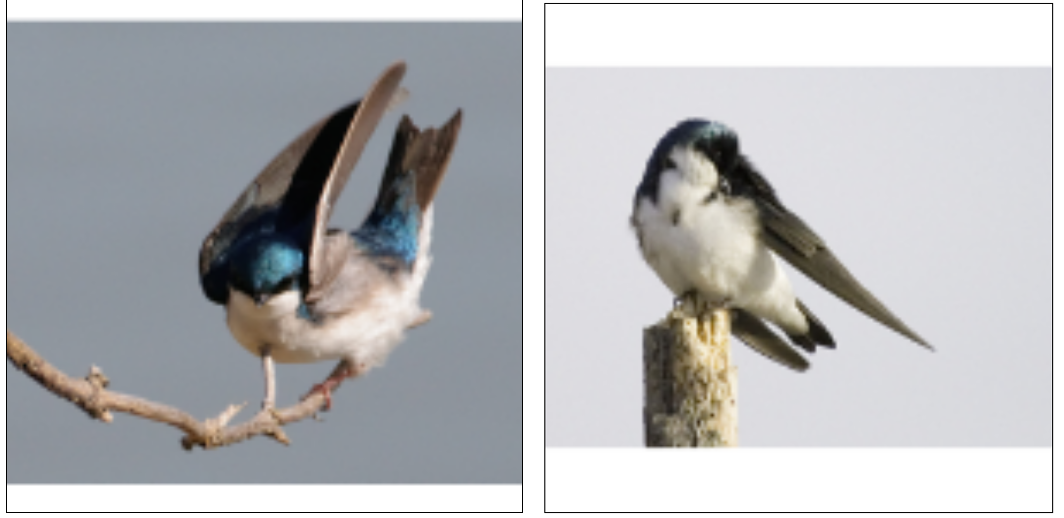
\includegraphics[ height=3cm, width=5.5cm]{\bilinearroot/figures/birds/birds_false_neg2.png}
    
    \end{tabular} 
    \\
    (a) & (b)


\end{tabular} 
\caption{Difficult re-identification cases in the CUHK03 dataset and the CUB-Birds dataset for the fine-grained classification~\citep{Wah11}. (a) -- the pairs of very similar images depicting different persons/bids species (b) -- the pairs of dissimilar images depicting the same person/bird species. There is a clear similarity between the challenges posed by the two tasks. Both re-identification and fine-grained classification deal with strong viewpoint variations, and often need to focus on small-scale fragments in order to distinguish subjects/classes. At the same time the re-identification task has a greater degree of alignment, and we therefore suggest a modification of the bilinear CNN exploiting the presenсe of such weak alignment in the re-identification case.}
\label{fig:teaser}
\end{figure*}

\textit{Fine-grained recognition tasks} are usually characterized by small visual differences between the categories and possibly large intra-category differences. The examples of the former are different bird species of similar color and pedestrians wearing similar clothes, the latter is often due to high variations caused by such factors as pose and lighting. 

The task of person re-identification shares considerable similarity with fine-grained categorization (see the example pairs in \fig{teaser}), as the matching process in both cases often needs to resort to the analysis of fine texture details and parts that are hard to localize. 

\textit{Bilinear convolutional neural networks} have been first suggested by \citep{lin2015bilinear} for fine-grained categorization tasks. The idea of this architecture is to utilize multiplicative interactions between different features computed using two feature extractor subnetworks. The intuition behind this suggests that such factorization may allow the model to learn such functions as detection (some parts may be detected, \eg{} birds beaks, heads) and recognition (\eg{} colors and textures). When the features carrying information about parts are combined in a  multiplicative way with the features carrying some texture information, the result may capture more complex concepts, \eg{} particular parts of particular color/texture.

The bilinear layer suggested by \citep{lin2015bilinear} is defined as follows:

\begin{equation}
   \label{eq:bilinear}
    x_{bilinear} = A^T B,
\end{equation}
where $A$ and $B$ are the outputs of the two deep feature extractors $f_A$ and $f_B$ (convolutional neural networks). $A \in \mathbb{R}^{S \times M}$, $B \in \mathbb{R}^{S \times N}$, $S$ is the number of spatial locations, $M$ and $N$ are the number of the featuremaps that the extractors $f_A$ and $f_B$ produce. The result of this operation is a matrix of size $M \times N$, but is reshaped to a vector $MN \times 1$.

Another characteristic that differs Bilinear CNNs from regular models is related to the way of handling the image spatial information. Non-bilinear architectures (\eg{} \citep{simonyan2014very}) apply fully-connected layers to the output of the last convolution layer to compute the final representation. In this case, each output element is computed by applying different weights to the input elements. It is easy to see that such operation may preserve some spatial information by assigning bigger weights for particular regions of the input feature maps. 

Bilinear CNNs, however, rather radically discard spatial information in the process of the sum-pooling. For very deep and powerful architectures like \citep{simonyan2014very}, such spatial information may be rather irrelevant and therefore can be easily discarded. In contrast, for more shallow architectures, like those that have been recently most popular for person re-identification, the radical pooling over all spatial locations may lead to a noticeable performance drop.

Moreover, as evidenced by the experiments of \citep{lin2015bilinear}, Bilinear CNNs with global pooling and powerful feature extractors are very appropriate for the tasks where pose variability may be very high, \eg{} bird species recognition  (for example of very different poses, see the lower picture in \fig{teaser}b). At the same time, the variability of geometric pose and viewpoints in re-identification problems is more restricted.

Thus the CNN architecture for person re-identification should be developed in the light of the discussed circumstances of this task, namely:
\begin{itemize}
    \item moderate-size architectures being used for person re-identification,
    \item more restricted pose variation of pedestrians, compared to other fine-grained recognition problems.
\end{itemize}
   
Given these preliminaries, it is appropriate to consider some intermediate variant that would preserve the features of both Bilinear and standard architectures. Indeed, such a variant, called Multi-region Bilinear CNN, is discussed later in this chapter. It can be regarded as a middle ground between the traditional CNNs and the Bilinear CNNs. In the experiments presented in this chapter, it is also shown that such a compromise achieves an optimal performance across a range of person re-identification benchmarks, while also performing favorably compared to the  previous state-of-the-art. The success of such architecture confirms the promise hold by deep architectures with multiplicative interactions such as Bilinear CNNs and the Multi-region Bilinear CNNs for hard pattern recognition tasks.

It should also be mentioned, that the Bilinear CNN with global pooling has been successfully applied to person re-identification by \citep{suh2018part} (after this work). The authors used powerful models of \citep{szegedy2015going} and \citep{cao2017realtime} (pre-trained for human pose estimation) for the recognition and detection streams correspondingly. This work presents some earlier (and lower) results, for which no explicit body part detection has been used. However, this work is the earliest to consider person re-identification a fine-grained problem and to adopt the Bilinear architecture for it. %discuss the results without pose estimation to our results?


%%%%%%%%% ABSTRACT
% \subsection{abstract}
% In this work we propose a new architecture for person re-identification. As the task of re-identification is inherently associated with embedding learning and non-rigid appearance description, our architecture is based on the deep bilinear convolutional network (Bilinear-CNN) that has been proposed recently for fine-grained classification of highly non-rigid objects. While the last stages of the original Bilinear-CNN architecture completely removes the geometric information from consideration by performing orderless pooling, we observe that a better embedding can be learned by performing bilinear pooling in a more local way, where each pooling is confined to a predefined region. Our architecture thus represents a compromise between traditional convolutional networks and bilinear CNNs and strikes a balance between rigid matching and completely ignoring spatial information.

% We perform the experimental validation of the new architecture on the three popular benchmark datasets (Market-1501, CUHK01, CUHK03), comparing it to baselines that include Bilinear-CNN as well as prior art. The new architecture outperforms the baseline on all three datasets, while performing better than state-of-the-art on two out of three. The code and the pretrained models of the approach can be found at \url{https://github.com/madkn/MultiregionBilinearCNN-ReId}.



%% !TEX root = ../Thesis_main.tex
\chapter{Introduction}

%video surveillance+
%person re-id+
% originates from Multi-Target Multi-Camera Tracking 
%open world / closed world+
%face : verification/identification
%common aspects: detection , processing, recognition
%deep learning

%retrieval
%fine-grained recognition
%adaptation

%datasets (cut from the papers) + table with reid dataset?
%architectures
%definitions?
%contribution - what is done
\section{Context}
\subsection{Problem of 3D reconstruction}

\subsection{Approaches for solving 3D Reconstruction problem}

Solutions for a reconstruction problem can be grouped in two major groups: 1) Geometric approach - when problem is represented as optimisation of scene state given constrains on projections of scene state to data, 2) Machine Learning approach - inverse model is optimisation.

If $X$ - is scene data, $z$ - is the state of the scene, and $g_i(z)$ - projection function of 3D scene $z$ state to perspective $i$, then to find an optimal 3D reconstruction, one solves this minimisation problem:
\begin{equation}
z_{rec} = \min_z\sum_i|X_i-g_i(z)|_2 .
\end{equation}

This approach only solves problem for once scene and does not provide any semantic information about it, only basic geometric information. 
The second approach is more modern and better fitted for machine learning applications, because instead of optimizing state of the scene, it's optimizes a model that performs computation from input data to some semantic (intrinsic) parameters, and can be described as following optimisation procedure:
\begin{equation}
\min_\theta\sum_i|X_i-g_i(f_\theta(\pi))|_2,\ \ \pi=I_\theta(\{X_i\}_i),\ \ z=f_\theta(\pi),
\end{equation}
where $\pi$ - are scene parameters, $f_\theta(\pi)$ - is a generative model that generates 3D state $z$ and it's function is determined by tunable parameters $\theta$.

In reconstruction process information can be introduced in two possible ways: 1) input signal - data measured by some spatial sensor, 2) by adding a priori knowledge while training the Inverse model or by design choice of reconstruction algprithm. Between the two source exist a fundamental trade-off and detirmination of which is dominant can be quite difficult \cite{tatarchenko2019single}.


\subsection{Objectives and Motivations}

The goal of this work to improve methods of 3D reconstruction in holistic context using deep learning systems. For efficient applications such as robotics in human environments and mixed reality more advanced machine perception systems are needed. Human perception is a complex system with several properties not all of which are replicated in modern machine perception systems. From cognitive sciences it's known that ability to model environments is one of the most important for perception system, in area of computer vision this is known as an ability to perform \textit{3D reconstruction} of scenes and environments. To solve this problem in a general case requires application of machine learning.

In particular, the development of such holistic deep 3D reconstruction system includes several important tasks:

\begin{itemize}
􏰀    \item Capturing scenes, complete with colour and depth data of a sufficient quality,
    \item Recalling objects from large scale database of objects,
    \item Segmenting variety of most common elements from sensor data, such as household objects and architectural components,
    \item Detecting and reconstructing shape and pose of and human bodies.
\end{itemize}

Each of these sub-tasks constitutes a challenge in the context of human perception.

The presence of noise in sensor data (e.g., consumer grade depth cameras) is a serious problem for all downstream sub-tasks, low fidelity of this data causes a considerable compaunding performance drop.

\subsection{3D data representations}

We can describe a 3D object in multiple ways, and codification of it's properties has ramifications about capturing different information about objects and scenes, as well as kinds of models that can regenerate them or computational resources needed to process it.
Each representation has it's own pros and cons. We assume 3D information representation to be positive effective and usefull if it captures more relevant information with less storage requirement (compression), increases signal to noise ratio of data, captures shape and texture properties with minimum trade-off.

Here are some popular examples of 3D data representations:
\begin{enumerate}
	\item Multiple 2D projections - captures surface texture, highly redundant representation if images overlap, also vulnerable to optic illusions.
	\item Voxels - simple, most of the time can be sparse, represents rough volumetric properties vell but losses most of surface properties.
	\item Point Cloud - are sparse in a sense that they don't capture empty space, losing all surface properties besides color and estimated normals and most of volumetric properties.
	\item 2.5D (RGB-D) images are widespread because of cheap measurement devices, capture volumentric depth but succeptable to occlusion of bodies in a scene and records a lot of noise with actual signal.
\end{enumerate}



%Motivation: RGB-D scanning is here and we want to have a fine-grained understanding of the 3D captures
In the recent years, a wide variety of consumer-grade RGB-D sensors, such as the Intel Real Sense, Microsoft Kinect, depth-sensor enabled smartphones, enabled inexpensive and rapid RGB-D data acquisition. Increasing availability of large, labeled datasets (e.g.,~\cite{chang2017matterport3d,dai2017scannet})  made possible development of deep learning methods for 3D object classification and semantic segmentation. At the same time, acquired 3D data is often incomplete and noisy; while one can identify and segment the objects in the scene, reconstructing high-quality geometry of objects remains a challenging problem.  

An example of the new approach in recent work 
\cite{avetisyan2019scan2cad}, uses a large dataset of clean, labeled geometric shapes
\cite{chang2015shapenet}, for classification/segmentation associating the input point or voxel data with object labels from the dataset, along with adapting geometry to 3D data.  This approach ensures that the output geometry has high quality, and is robust with respect to noise and missing data in the input.  
At the same time, a ``flat'' classification/segmentation approach, with each object in the database corresponding to a separate label and matched to a subpart of the input data corresponding to the whole object, does not scale well as the number of classes grows and often runs into difficulties in the cases of extreme occlusion (only a relatively small part of an object is visible). 
Significant improvements can be achieved by considering object \emph{parts}, or more generally part hierarchies. 
Part-based segmentation of 3D datasets promises to offer a significant improvement both in finding the best matching shape in the dataset, recognizing objects from  highly incomplete data (e.g., from a couple of parts) from  as well as more precise geometry adaptation as well as, potentially, assembly of new shapes out of existing parts yielding a closer match to the input data. 

large collection of 3D models in database can be reduced to structured representations, 
objects with occluded sub-parts still can be recognized by parts available in the scan and the rest can be guessed with high probability, using parts, we can reconstruct new objects that are not yet present in the database of shapes.

Based on different approaches for volumetric information integration, from enhancements of  methods such as volumetric fusion \cite{curless1996volumetric}, to probabilistic  methods, and plethora of methods based on their combinations.

Compared to computer graphics models manually created by 3D professionals, 3D scans are noisy and incomplete.
Amount of noise and limited resolution of consumer-grade scanning hardware pose significant challenges for solving this important problem of scene reconstruction. 
Approaches of reconstruction based on fitting existing 3D assets into scene scans, have shown a lot of promise but still had problems with finding exact models from large database such as ShapeNet \cite{chang2015shapenet}, because of occlusion and lack of spatial context.

Learning-based approaches are very good at extracting features representative of objects and scenes as a whole, allowing to fill in occluded areas or guess parts affected by noise \cite{dai2017shape,dai2018scancomplete,song2017semantic}. These features are sufficient for scene completion, but they are not as good at recovering geometric primitives like: sharp edges, planar surfaces or borders between sub-parts, resulting in reconstruction quality much poorer than that of 3D content created by humans.

In this work, we focus on the key problem of semantic part segmentation of objects in the scenes, enabling further improvements in  dataset-based reconstruction. 
Semantic part-segmentation, can help in these situations, when sufficient number of the object parts is visible model can infer the non-visible parts essentially completing an object in sense of maximum probability conditioned on input data.

In human-made environments, a lot of objects have naturally defined semantic sub-parts, and those sub-parts can, in turn, have their sub-parts, i.e., parts form \emph{hierarchies}.  In our work, we use scene and object representation based on such part hierarchies.  We show how a part-labeled dataset of scanned 3D data suitable for machine learning applications can be constructed, and used to improve the performance of segmentation algorithms. 

Definitions of sub-parts are based on a set of primitive elements that were manufactured by one formation method or from one material.

Because of that and the fact that static scenes have other relationships between objects (fixed to each other or in direct surface contact), it's reasonable to suggest a scene description format that possesses a property of hierarchy (e.g., trees or other kinds of graphs).
Representing scenes as a discrete structures with multiple relationships between nodes. Such relationships like composability of its parts and affordances between whole objects, in turn allowing to compose a scene from separate objects.

\todo{merge these paragraphs}

In domain of human-made environments a lot of objects have sub-parts and those sub-parts can in turn have their own sub-parts. Definition of sub-part is often based on a set of primitive elements that were manufactured by one formation method or from one material. Because of that and the fact that static scenes have other relationships between objects (fixed to each other or in direct surface contact), it's reasonable to suggest a scene description format that possess a property of hierarchy (e.g. trees or other subgraphs).
A lot of researchers over the last 20 years came to the same conclusion. A lot of work on that problem was done by Mumford and Zhu in \cite{zhu2006stochastic}.

One of the papers dealt with problem of modeling Images as a hierarchy of super-pixels. \cite{russell2009associative}, or as a tree of geometric primitives (e.g. cylinders, spheres or 3D boxes) \cite{li2017grass}.

% point cloud (PC) turned in to a graph (based on proximity) point-cloud parser network reduces number of nodes and edges and enriches their feature vectors. First part of the decoder network functions similar to Feature Pyramid Network in CNNs, which performs local computations on different scales, followed by "pooling or convolutions" with reduced spatial component and increased feature components, thus leaving only small number of "keypoints" required to outline shapes of objects.



CAD constructor network translates that graph into CAD object (tree with primitives and combination rules). CAD rendered makes a mesh out of that object thus a residual between original PC and Mesh can be calculated.

Proximity Graphs - concept that allows to build a bridge between Point Clouds and Graph Processing. This area of computational geometry has a lot of theoretical results to offer for Deep Learning piplene designer.


\subsection{Definitions and examples}
\subsection{Data sources and devices}

\section{Inverse Graphics Problem formulation}

\cite{rezende2016unsupervised,eslami2016attend,kulkarni2015deep,wu20153d,izadinia2017im2cad}

Inverse graphics approach enables to solve a problem of "real-world" scene understanding through reconstruction of that scene and comparison it to measured data in some form.

Because it's a fairly new method it has some unexplored facets:
\begin{enumerate}
    \item How can we scale to hundreds and thousands of objects with different parameters.
    \item Embedded representations better than procedural generation
    \item Are there format that can have all advantages of CAD models and probabilistic properties that arise from real-world uncertainties.
\end{enumerate}

Central goals of computational perception is to get structured description of scenes from measurements such as photographic images, scans and videos.

Computer Vision as Inverse Graphics is the most rational formulations that could help us achieve this goal.

In the past, it has been hard to directly solve these problems in practice because of computational limitations.

However, it may be right time to take another look at this idea due to significant advances in deep learning for computer vision, probabilistic programming, and computer graphics.

Probabilistic programming - a tool that allows us to implement complex models while keeping ability to perform inference, extend with other probabilistic models by being general-purpose.

Re-formalizing inverse graphics in terms of probabilistic programming and deep learning allow us to solve even more complicated vision problems with off-the-shelf computational technology.

To make this approach scalable, my research can incorporate effective techniques such as: approximate Bayesian computation, differentiable programming for rendering.

Computer Graphics nowadays seems to be improving at a great pace in terms of designing solutions for hard image synthesis problems, but these solutions are usually hand-made and not flexible enough to cover all needs for general-purpose real world object generating, latest advances in generative models can help with that.


\subsection{Overcoming lack of information}

\section{Datasets}

Only recently research community started accumuulating sugnifficant amount of algined sensor data to solve large scale 3D reconstruction problems in deep learning context. In last 4 years we saw an explosion of 3D shape databases and 2D-to-3D indoor scene datasets, such as ShapeNet, 2D-3D Semantic, Scannet and Matterport3D datasets. Because accuracy and reacall properties of deep learning models scale with amount and variety of data, number of state-of-the-art models grew as well.

\section{Architectures}

PanopticFusion~\cite{narita2019panopticfusion} is a model that is able to segment large indoor scenes and separate \textit{Stuff} and \textit{Things}.


For outdoor datasets Point Cloud representation of data is more common because of large empty spaces and the way LiDAR sensor collects data. In such setting instance segmentation is nessesary first step for reconstruction~\cite{zhang2020instance}.

\subsection{Multi-view models}

Detailed comparision of multi-view 2D CNN model and 3D volumetric CNN can be found in \cite{qi2016volumetric}.

\subsection{Implicit 2D models}

Like inverse graphics network. Model takes 2D images and returns 2D images with 3D properties changed. 

\subsection{3D convolutional models}

Model generates or processes voxel image with 3D convolutional operation implemented Dense or Sparse.

Semantic information can boost the reconstruction performance because deep learning systems are able to pick up onto consistent signal \cite{jiao2018look,tatarchenko2019single,kendall2018multi}.

\subsection{2D to 3D Projection models}

Model uses camera parameters to compute 3D representation using 2D/2.5D images and projection operation.

\subsection{Point Set layers}

Neural Network processes a set of points to classify, segment or predict new set of points.

\subsection{Graph-Convolutional layers}

Model processes Geometric Graph where nodes represent points registered on a surface of objects or parts of objects, and has geometric or other information representing edges between points. Layers process activations associated with nodes taking into account the connectivity.

\subsection{Differentiable rendering layers}

Rendering operation is implemented in a differentiable way, allowing backpropogation of gradient information from 2D images to meshes and textures of the objects being rendered.

\subsection{Mesh generating layers}

Neaural Network layers that can create a mesh by way of processing a template 3D shape with parametracised operation or meshing other 3D shape representation generated by computation from weights and input.

\subsection{Implicit 3D models}

Models like NeRF, PIFU3D, neural network implements a rendering function depending on view angle and other graphics parameters, one model represents one scene and don't generalise for viriety of scene inputs.



\section{Contributions}

% \chapt{hist}, \chapt{bilinear} and \chapt{gradrev} use  person re-identification architecture of \citep{Yi14} as a baseline method (it is also  described in \sect{intro_architectures}).  \chapt{bilinear} is based on the results of \chapt{hist}: the loss function introduced in \chapt{hist} is used for 
% all the experiments in \chapt{bilinear} as it was demonstrated to show the best performance for person re-identification. 
% The results of \chapt{gradrev} were chronologically the earliest among all the results presented in this work, therefore  methods  from \chapt{hist} and \chapt{bilinear} were not used there. 
% Although the contributions of each of the chapters are independent, they are all parts of building a person re-identification pipeline and can be applied simultaneously. 
% \chapt{wildface} considers domain adaptation for surveillance face recognition and uses the method from \chapt{gradrev} as one of the baselines.
 




% \begin{figure*}[t]%{R}{0.5\textwidth}
% \centering

% \begin{tabular}{c c}

% \begin{tabular}{c c c c}

% 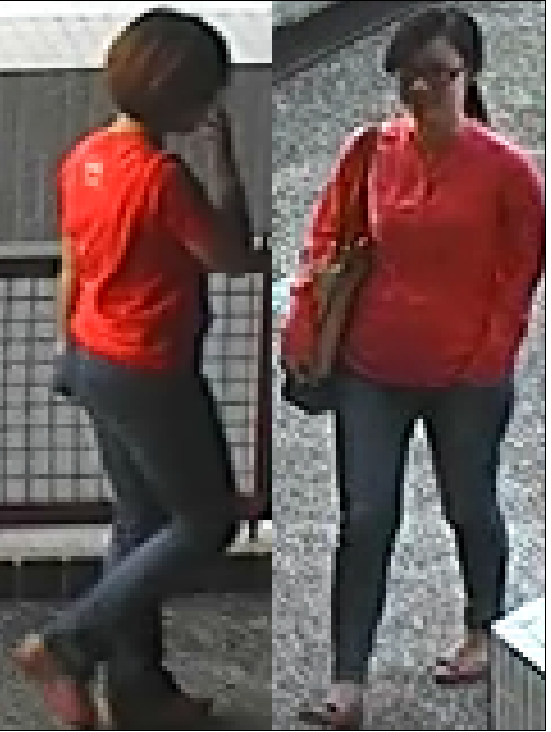
\includegraphics[ height=2cm, width=1.2cm]{\bilinearroot/figures/pedestrians_pairs/false_pos1.png}&
% 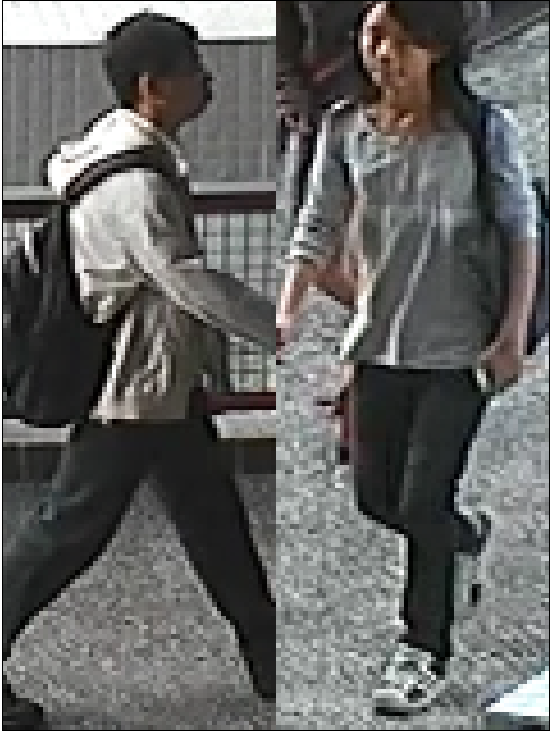
\includegraphics[ height=2cm, width=1.2cm]{\bilinearroot/figures/pedestrians_pairs/false_pos2.png}&
% 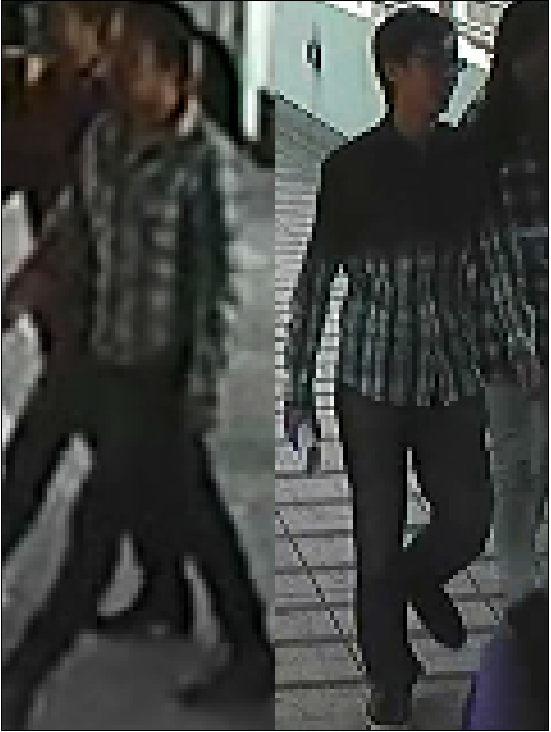
\includegraphics[ height=2cm, width=1.2cm]{\bilinearroot/figures/pedestrians_pairs/false_pos3.png}&
% 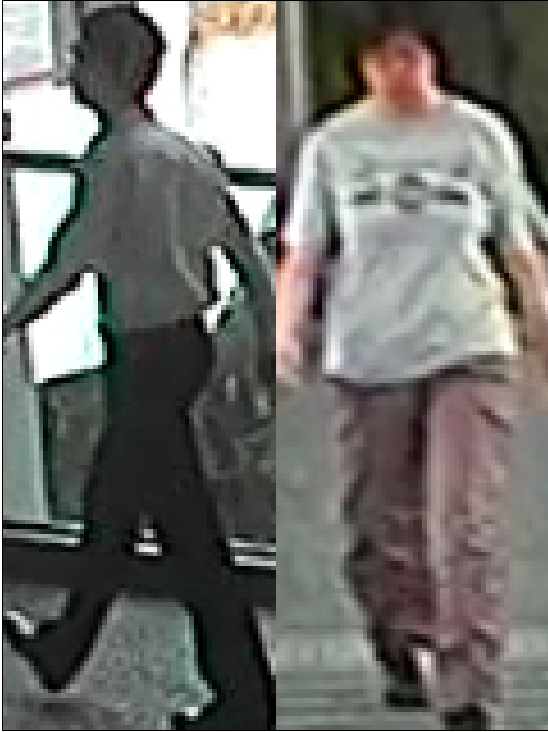
\includegraphics[ height=2cm, width=1.2cm]{\bilinearroot/figures/pedestrians_pairs/false_pos4.png}
% \\
% 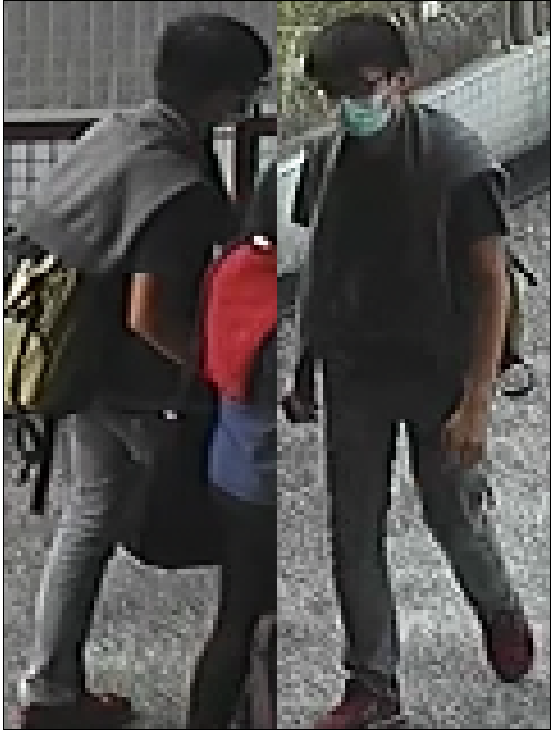
\includegraphics[ height=2cm, width=1.2cm]{\bilinearroot/figures/pedestrians_pairs/false_neg1.png}&
% 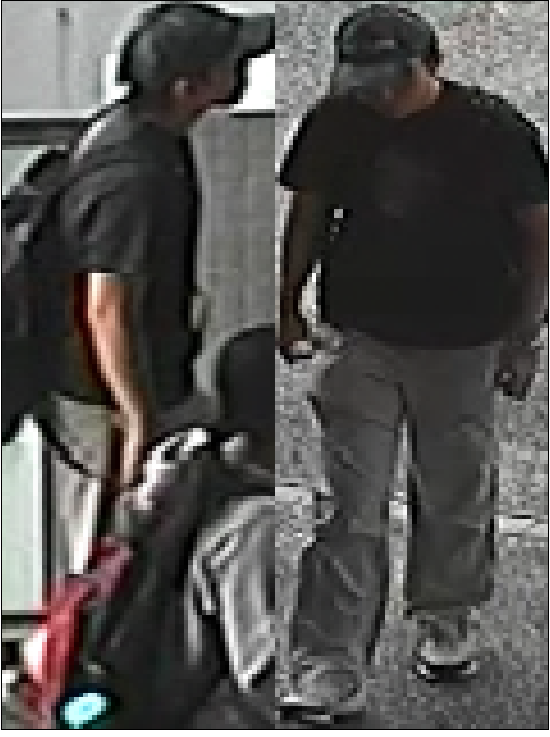
\includegraphics[ height=2cm, width=1.2cm]{\bilinearroot/figures/pedestrians_pairs/false_neg2.png}&
% 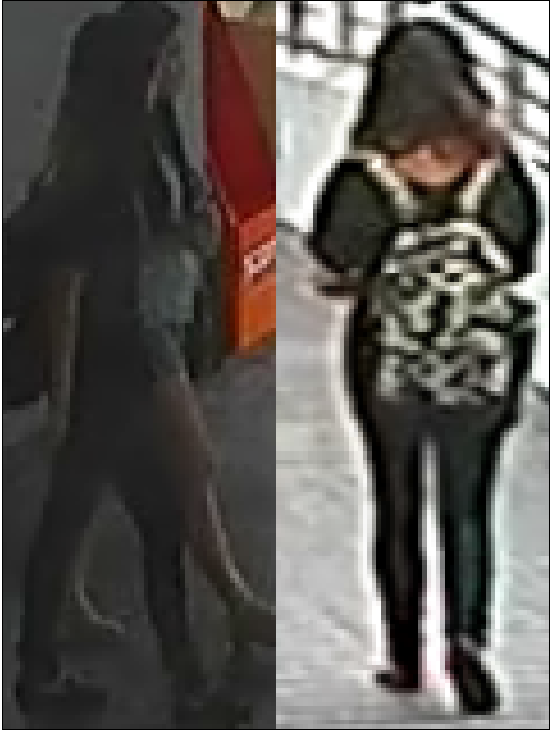
\includegraphics[ height=2cm, width=1.2cm]{\bilinearroot/figures/pedestrians_pairs/false_neg3.png}&
% 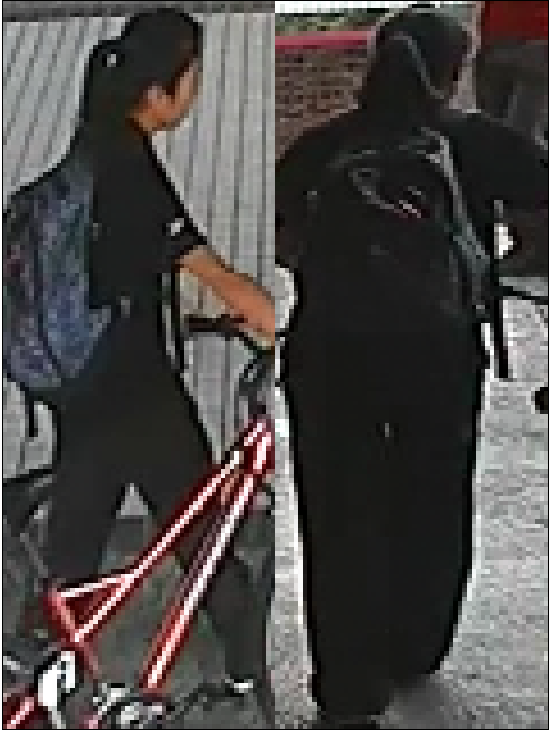
\includegraphics[ height=2cm, width=1.2cm]{\bilinearroot/figures/pedestrians_pairs/false_neg4.png}
% \end{tabular} &
% \begin{tabular}{c c}
% 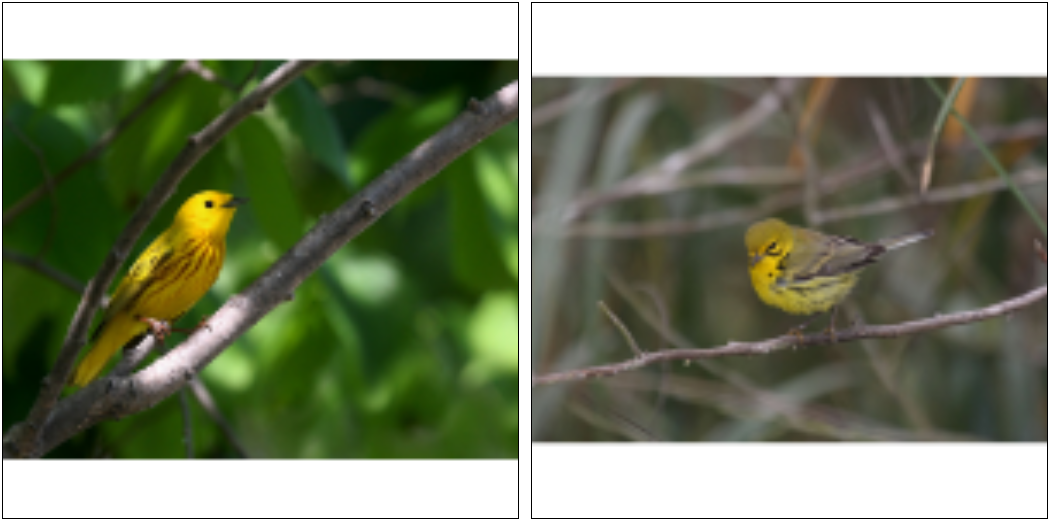
\includegraphics[ height=2cm, width=4cm]{\bilinearroot/figures/birds/birds_false_pos1.png}&
% 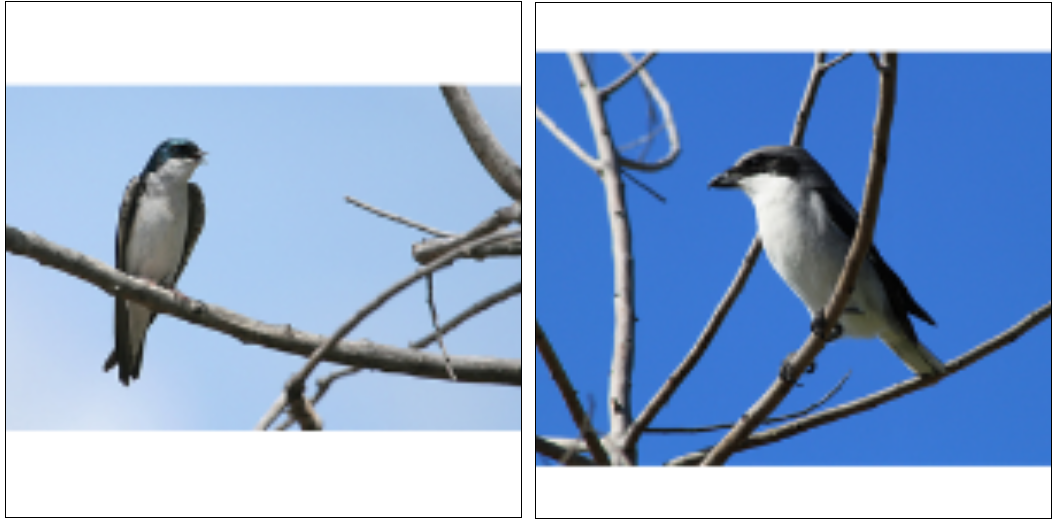
\includegraphics[ height=2cm, width=4cm]{\bilinearroot/figures/birds/birds_false_pos2.png}


% \\
% 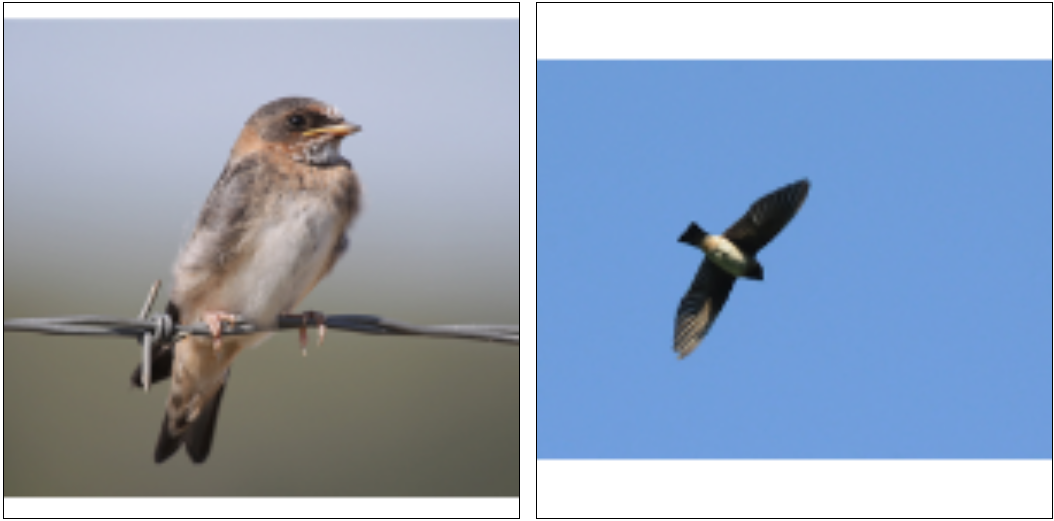
\includegraphics[ height=2cm, width=4cm]{\bilinearroot/figures/birds/birds_false_neg1.png}&
% 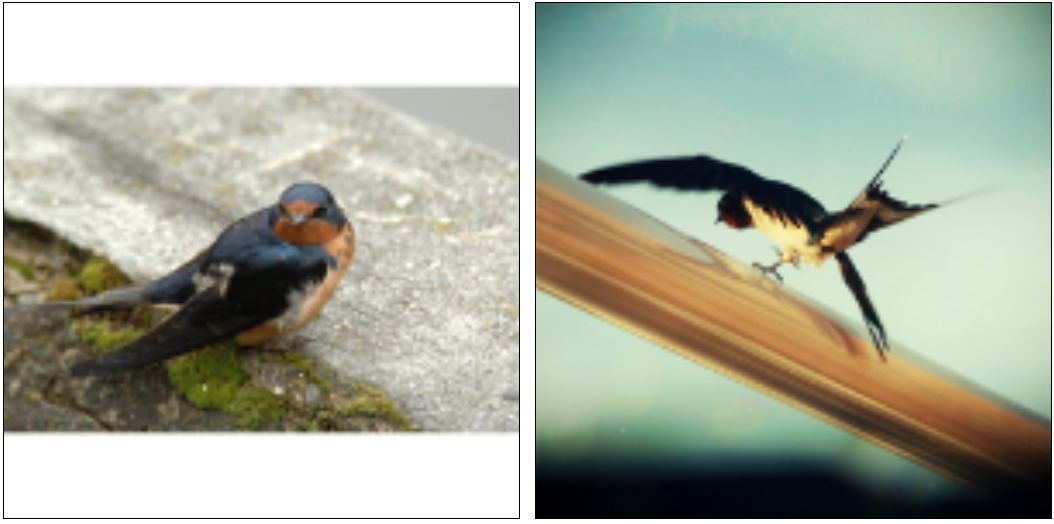
\includegraphics[ height=2cm, width=4cm]{\bilinearroot/figures/birds/birds_false_neg3.png}

% \end{tabular}
% \end{tabular} 
% \caption{Left-- difficult re-identification cases in the CUHK03 dataset \citep{li2014deepreid}. The pairs in the upper row show very similar images depicting different persons, the pairs in the lower row show dissimilar images depicting the same person. Right -- analogous cases for the CUB-Birds dataset for the fine-grained classification~\citep{Wah11}. There is a clear similarity between the challenges posed by the two tasks. Both re-identification and fine-grained classification deal with strong viewpoint variations, and often need to focus on small-scale fragments in order to distinguish subjects/classes. At the same time the re-identification task has a greater degree of alignment, and we therefore suggest a modification of the bilinear CNN exploiting the presenсe of such weak alignment in the re-identification case.}
% \label{fig:teaser}
% \end{figure*}


\begin{figure*}
\begin{center}
    

\begin{tabular}{c}
 
    
            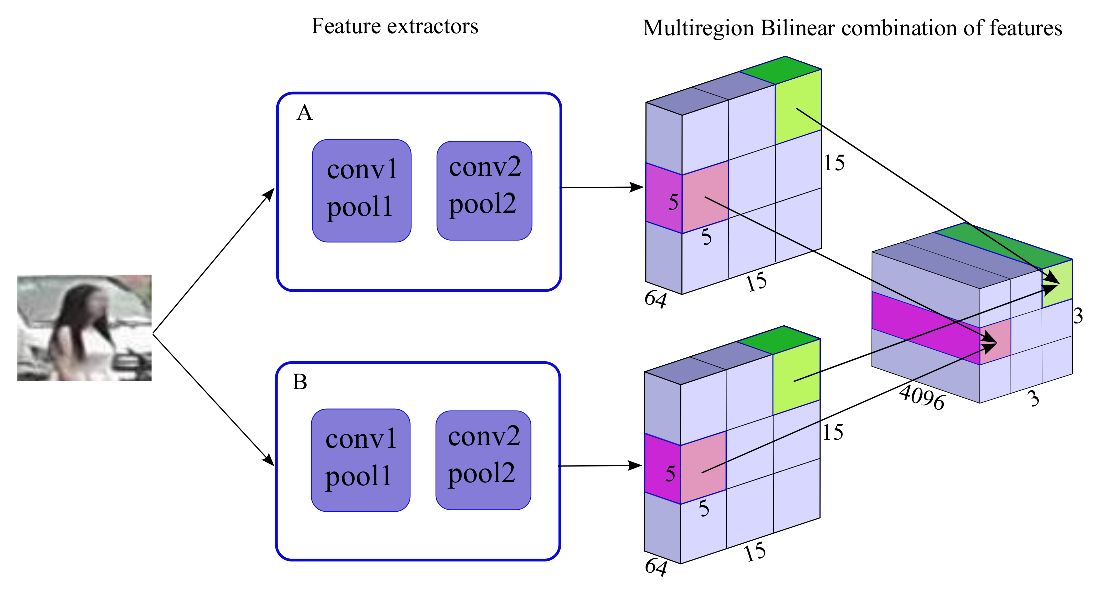
\includegraphics[width=0.7\textwidth]{\bilinearroot/figures/architecture/multiregion_bilinear.eps}\\
    (a)\\
            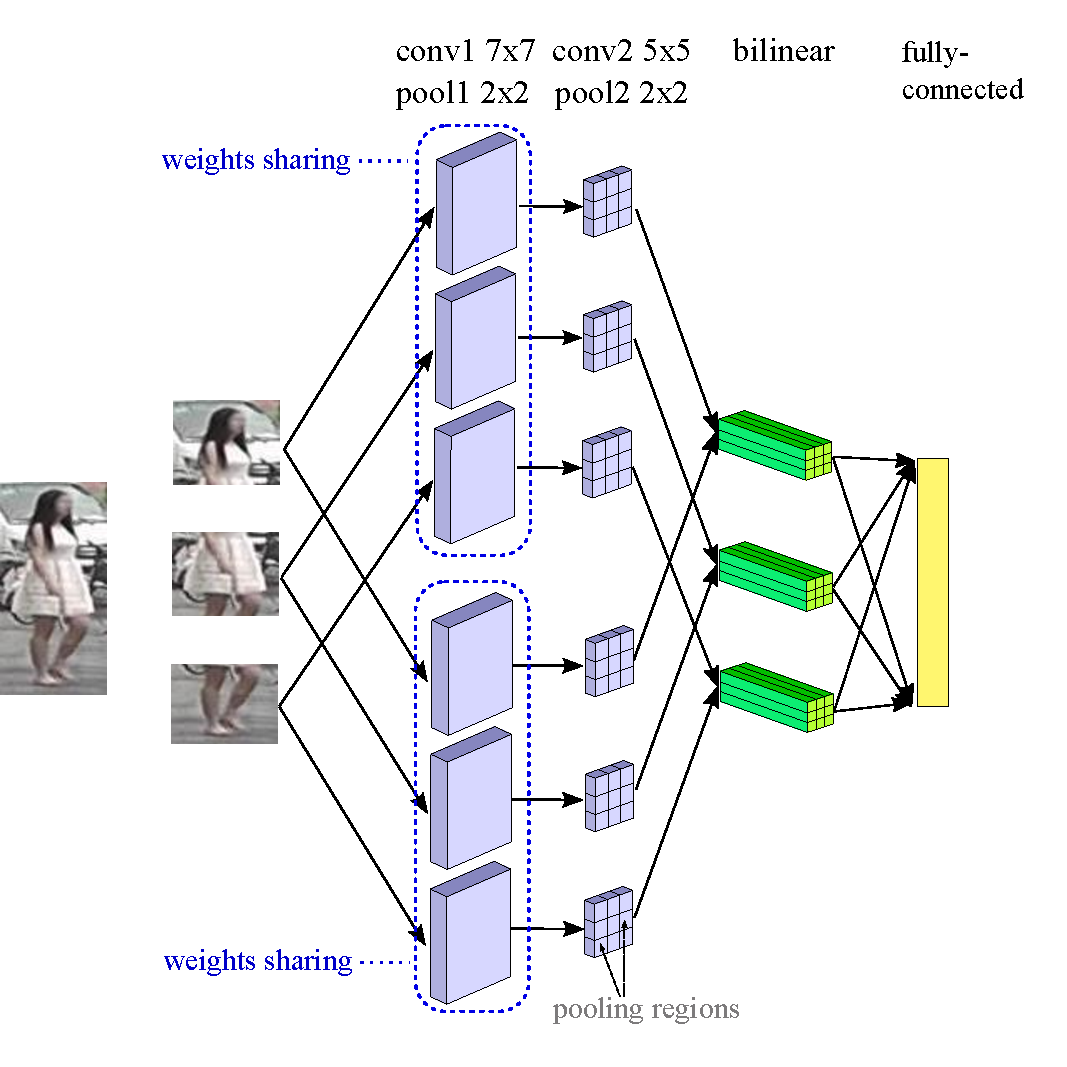
\includegraphics[width=0.7\textwidth]{\bilinearroot/figures/architecture/architecture.pdf}
            \\
    (b)\\
   
 \end{tabular}
        \caption{The proposed architecture for person re-identification: (a) - multi-region bilinear sub-network used for each of the three parts of the input image, (b) - the whole multi-region Bilinear CNN architecture that uses bilinear pooling over regions rather than the entire image. The new architecture achieves state-of-the-art performance over a range of benchmark datasets.}
        \label{fig:architecture}
    \end{center}
\end{figure*}

%\section{Related work}
\label{sect:related}

There are two main research directions dedicated to face recognition for low-quality data: (i) the face restoration approach and (ii) the domain adaptation approach. In the face restoration-based approach, low-quality images are enhanced and restored to facilitate recognition. The ability to reuse existing recognition systems that were developed for high-quality data comes as a natural benefit of such methods. Domain adaptation methods are conversely aimed to change the existing recognition systems so that they are better suited for the target domain (i.e.\ low resolution/quality images). We now provide a brief review of both approaches.

\subsection{Face restoration methods}

There is a vast range of methods that perform face restoration. In most of them, different degradation types are considered separately. Pan \textit{et al.} \cite{pan2014deblurring} propose an effective face deblurring method based on approximating blur kernel followed by non-blind deconvolution. The blur kernel  approximation is guided by the known non-blurred exemplar with the structure similar to the input image structure. 

In Zhang \textit{et al.}~\cite{ZhangYZNH11}, deblurring and recognition tasks are considered simultaneously. They use a sparse representation of the input image in terms of the gallery image set. The blur kernel and representation coefficients are estimated iteratively. Classification is finally performed based on the classes with the highest coefficients in the sparse representation.  


A number of recent methods \cite{TuzelTH16,ZhuLLT16,xu2017learning,huang2017wavelet} explore the task of restoration of extremely low-resolution images using deep neural networks. All these works utilize the paired (aligned) learning scheme, where the high-resolution ground truth is known for every low-resolution image in the training set. The low-resolution training data are simulated using synthetic degradation of the initial high-resolution images. In \cite{xu2017learning} and \cite{TuzelTH16}, a generative adversarial network~(GAN)~\cite{goodfellow2014generative} is used to force the restoration network to produce more natural images. In \cite{huang2017wavelet}, an additional structure-based loss that uses wavelet transform is suggested for the same goal. While the results of these methods are impressive, there is no direct way to use the paired learning approaches for the arbitrary combination of degradation factors that one may encounter when analyzing real images captured by surveillance cameras. 

\subsection{Domain adaptation methods}

Several recent works are dedicated to domain adaptation in the context of different recognition tasks \cite{Volpi_2018_CVPR,Hong_2018_CVPR,Deng_2018_CVPR,Bousmalis_2017_CVPR,Murez_2018_CVPR}. In \cite{Murez_2018_CVPR}, 
\cite{Bousmalis_2017_CVPR} and \cite{Deng_2018_CVPR}, image-level domain adaptation is performed for segmentation, classification and similarity learning (person re-identification) correspondingly. Hong \textit{et al.} \cite{Hong_2018_CVPR} and Volpi \textit{et al.} \cite{Volpi_2018_CVPR} resort to feature-level domain adaptation for segmentation and classfication tasks. Both feature-level and image-level techniques are used in \cite{Hoffman17}.

Some of the aforementioned methods \cite{Hoffman17,Deng_2018_CVPR,Murez_2018_CVPR} employ CycleGAN framework  to change the domain of training data for classification, segmentation, and person re-identification. Here we explore a similar approach for the task of face recognition in the presence of complex degradation factors.

Hong \textit{et al.} \cite{HongIRY17} and
Sohn \textit{et al.} \cite{SohnLZY0C17} approach face recognition tasks for low-quality image domain. They consider image degradation as a domain shift and perform feature-level unsupervised domain adaptation based on adversarial learning showing better recognition results. 
The works \cite{HongIRY17} and \cite{SohnLZY0C17} are very related to ours: the authors show that domain-specific data augmentation is essential for training face recognition systems. 
 However, in both works, the data augmentation is performed 'by hand' (the degradation types and hyper-parameters for transforms are chosen and fixed), while we augment the training data in an automatic manner utilizing the CycleGAN framework, which can also be viewed as an image-level domain adaptation.
%Additionally, in contrast to \cite{HongIRY17}, we do not consider extremely large pose variation. Instead, we are more focused on the image degradation factors (e.g. the combination of small size, blur, JPEG-compression). 
Differently from \cite{SohnLZY0C17}, where evaluation is performed for the Youtube faces dataset, we approach the task in the presence of the somewhat stronger domain shift, as our test data are captured by surveillance cameras and are mostly of much lower quality.




%Some works already successfully use CycleGAN technique to perform an unsupervised domain adaptation. \cite{CYCADA} approached semantic segmentation. % add avput CYCADA

%recognition and reconstruction approaches
% Several existing works consider restoration and recognition problems jointly. In some works, authors apply the recognition-based priors to achieve better restoration results. \cite{TODO , Xu} 

% There are also approaches jointly performing explicit recognition and restoration
% In \cite{TODO Close  the  loop:  Jointblind  image  restoration  and  recognition  with sparse representation prior , Baker} The  proposed  approaches  perform  recognition  using  a  limited  number  of  gallery  images.   In parallel, they reconstruct the input image and classify it based on labels of the most relevant examples found in the train set.

 
% One of the baselines used in this work applies the similar scheme: CycleGAN framework is used to transfer the low-quality test data into the high-quality domain, the domain classifier serves as 'restoration' loss. We additionally introduce the recognition component into this scheme: another baseline is the same CycleGAN but with domain classifier based that is learned using features calculated with the pre-trained face recognition network.




\section{Evaluated approaches}
\label{sect:method}
\bigskip
\indent\textbf{Face recognition for the low-quality image domain}\\
%\subsubsection{Face recognition for the low-quality image domain}
\label{sect:strategies}
In this work we consider and compare two main approaches to face recognition for surveillance data: 1) restoration-based approach and 2) domain adaptation of existing face recognition neural networks. 

We consider two facial image domains: \begin{itemize}
\item domain $T: \{X^{T}_{i} \}_{i=0}^{N_T}$ that includes low-quality facial images $X^{T}_{i}$ captured using surveillance cameras. Usually, there are no identity labels provided, as assigning identity labels is quite challenging and may not even be feasible.
\item domain $S: \{(X^{S}_{i}, Y^{S}_{i})\}_{i=0}^{N_S}$ that includes facial images $X^{S}_{i}$ harvested from the Internet. These images are usually of higher quality and are taken in good lighting conditions. We assume that the data in this domain are supplied with identity labels $Y_i$.
\end{itemize}  

According to the available labeling, we can consider two different pipelines for building face recognition systems for surveillance data. The first option is the restoration-based approach when we use transform $F^{T \rightarrow S}: T \longrightarrow S$ as a face restoration method and then apply existing recognition neural network $R^{S}$ that is pre-trained on images from the domain $S$. The second option is to use the transform $F^{S \rightarrow T}: S \longrightarrow T$ to transfer the large collections of labeled training data to the target domain of surveillance images. In this scenario, we retrain the existing face recognition networks resulting in the new adapted model $R^{T}$.

More formally, we consider the following two pipelines for face recognition in the domain $T$.  We denote $d^{T}$ and $d^{S}$ the descriptors produced by the domain-specific face recognition models $R^{T}$ and $R^{S}$. These descriptors may be used e.g.\ to identify matching and non-matching faces based on the distances between them. 
 
$F^{T \rightarrow S}: T \longrightarrow S$ and $F^{S \rightarrow T}: B \longrightarrow A$ are the image-level domain transfer mappings. In the restoration-based approach, we train the recognition model $R^{S}$ using labeled data  $\{(X^{S}_{i}, Y^{S}_{i})\}$ where $X^{S}_{i} \subseteq B$. We then test the learned model by computing the descriptors $d^{S}$ after applying the network $F^{T \rightarrow S}$:  $d^{S} = R^{S}(X^{T\rightarrow S}) = R^{S}(F^{T \rightarrow S}(X^{T}))$

In the domain adaptation approach, we train the recognition network $R^{T}$ using labeled data $\{(X^{S \rightarrow T}_{i}, Y^{S}_{i})\}$, where the training examples $X^{S \rightarrow T }_{i} = F^{S \rightarrow T}(X^{S}_i)$, $X^{S}_i \subseteq S$ are obtained by transforming the high-quality images to the low-quality domain using the learned transformation $F^{S \rightarrow T}$. In this case, we apply the learned network directly to the low-quality images by computing and working with their descriptors $d^{T} = R^{T}(X^{T})$. The two approaches are compared below.


%image describing train and test time for both schemes
\bigskip
\indent\textbf{Learning domain transfer mappings}\\
%\subsubsection{Learning domain transfer mappings}
\label{sect:domain_transfer}
We use the CycleGAN approach~\citep{ZhuPIE17} to simultaneously learn the domain transfer mappings in both directions: $ F^{T \rightarrow S}: T  \longrightarrow S$ (restoration-based approach) and  $F^{S \rightarrow T}: S \longrightarrow T$ (domain adaptation approach). Here we describe the objective functions used for learning the domain transfer architecture.

We use the variant of CycleGAN similar to the one introduced in \citep{LiuNIPS2017} as we found it resulting in more stable and visually more plausible results for our task than the original framework \citep{ZhuPIE17}. Following \citep{LiuNIPS2017}, we decompose the domain transfer mappings into the compositions of encoders and generators: $F^{T \rightarrow S} = G^{S} \odot E^{T} $ and $F^{S \rightarrow T} = G^{T} \odot E^{S} $. Here, the encoders $E^{T}$ and $E^{S}$ transfer input images to the latent space, and generators $G^{S}$ and $G^{T}$ map the input latent codes to the domains $S$ and $T$.
 
For inputs $X^{T} \subseteq T $ and $X^{S} \subseteq S $ the results of their transfer to the opposite domain will be:
\begin{equation}
    X^{T \rightarrow S} = F^{T \rightarrow S}(X^{T}; \theta^{T}_F) = G^{S}(E^{T}(X^{T}))  
\end{equation}
\begin{equation}
    X^{S \rightarrow T} = F^{S \rightarrow T}(X^{S}; \theta^{S}_F) = G^{T}(E^{S}(X^{S}))
\end{equation}

The objective function used by the CycleGAN approach for learning is composed of the two symmetric parts:
\begin{equation}
\mathcal{L} = \mathcal{L}^{T} + \mathcal{L}^{S},
\end{equation} where $\mathcal{L}^{T}$ further decomposes as:
\begin{equation}\label{eq:domain_loss}
     \mathcal{L}^{T} = \mathcal{L}_{\text{GAN}}^T + \lambda_1 \mathcal{L}_{\text{cycle}}^T + \lambda_2 \mathcal{L}_{\text{rec}}^T,
\end{equation}
while $\mathcal{L}^{S}$ has same structure as $\mathcal{L}^{T}$:
\begin{equation}\label{eq:domain_loss2}
     \mathcal{L}^{S} = \mathcal{L}_{\text{GAN}}^S + \lambda_1 \mathcal{L}_{\text{cycle}}^S + \lambda_2 \mathcal{L}_{\text{rec}}^S,
\end{equation}


We now describe each of the terms in \eq{domain_loss}.
The GAN loss serves as the optimization objective for the domain transfer: 

\begin{dmath}
\mathcal{L}_{\text{GAN}}^A = 
    \min_{\theta^{S}_F} \max_{\theta^{T}_D} \mathbb{E}_{x \sim p_{X^{T}}} \log D^{T}(x) +
    \mathbb{E}_{x \sim p_{X^{S}}} \log \big(1 - D^{T}(F^{S \rightarrow T}(x)) \big)\,
\end{dmath}


Here, $D^{T}(X;\theta^{T}_D)$ and $D^{S}(X;\theta^{S}_D)$ are discriminators for the domains $T$ and $S$ that are trained in parallel with the training of the domain transforms.

The other two terms are the so-called cycle consistency loss: 
\begin{equation}
\mathcal{L}_{\text{cycle}}^T = L_1(F^{S \rightarrow T}(F^{T \rightarrow S}(X^{T})), X^{T})  
\end{equation}
and the reconstruction loss:
\begin{equation}
\mathcal{L}_{\text{rec}}^T = L_1(G^{T}(E^{T}(X^{T})), X^{T}) 
\end{equation}
In both terms, $L_1(\cdot,\cdot)$ denotes the $L_1$ distance.

We show the results of transferring the Internet and surveillance images to the other domain in figure \ref{fig:lr_hr_gan_res_ytube_initial_degraded}. While these results look interesting, we do not analyze their visual quality, as we are ultimately interested in the recognition performance rather than obtained visually-convincing images.

\bigskip
\indent\textbf{Learning face recognition models}\\
%\subsubsection{Learning face recognition models}
\label{sect:face_recognition}
In both scenarios that we compare in this paper, we need to train a face recognition model that turns images into vectorial descriptors. This happens either in domain $S$ (in the face restoration approach) or in domain $T$ (in the domain adaptation approach).

In either case, the goal of the training is to build a deep convolutional network that converts face images to the descriptors, such that matching face images have close descriptors and non-matching face descriptors have dissimilar descriptors. We use the Binomial Deviance loss~\citep{Yi14} to perform such training \eq{bindev}. We note that the choice of a particular metric learning loss is orthogonal to our study.

Alternatively to the models trained using the setting discussed above, we also consider reusing the VGG face model trained by the authors of~\citep{parkhi2015deep} on the VGG-face dataset.
\section{Experiments}
\label{sec:4}
\subsection{ModelNet40 dataset}
In our experiments we used well known data set of 3D objects ModelNet40.
It is a subset of 40 classes of larger data set called ModelNet \cite{wu20153d} that contains different 3D CAD models in OFF format.

The total size of ModelNet40 data set $12311$.
The data set is split into training and test subsets, their sizes are $9843$ and $2468$ correspondingly.
The data set is not balanced.
Number of samples per class vary: from 64 to 889, see Figure \ref{fig:modelnet_classes}.

\begin{figure}
	\centering
    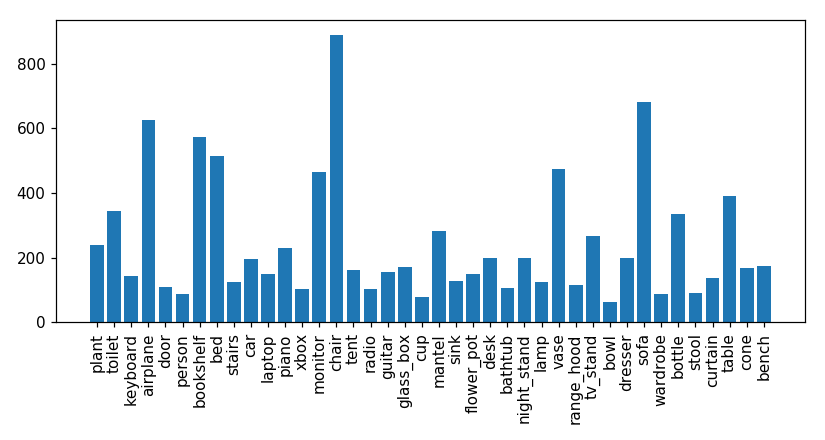
\includegraphics[width=\textwidth]{Figures/shape_retrieval/modelnet_classes.png}
    \caption{ModelNet40 data set: distribution of samples per class.}
    \label{fig:modelnet_classes}
\end{figure}

\subsection{Implementation details}
To demonstrate the impact that the triplet based training has on the performance of CNN descriptors
we use a deep network architecture shown in a Table~\ref{tab:net-architecture}. This network was implemented in PySparseConvNet, which is our modification of the SparseConvNet library \cite{graham2014spatially}. Besides new loss functions PySparseConvNet can be accessed from Python for a more interactive usage.

When forming a triplet for training we choose uniformly randomly a positive pair of objects from one class
and select a negative sample uniformly randomly from one of other classes.

For the optimization we use the SGD \cite{bottou-tricks-2012}, and the training is done
\begin{itemize}
\item in batches of size from $45$ to $90$ depending on a GPU video memory,
\item with a learning rate of $0.002$,
\item and a momentum equal to $0.99$.
\end{itemize}
Training can take up to a week on a server with advanced GPU, such as NVIDIA Titan X or GTX980ti.

\begin{figure}
\centering
\begin{tabular}{ccccc}
  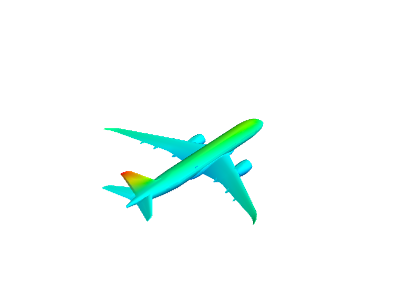
\includegraphics[width=0.19\columnwidth]{Figures/shape_retrieval/pic_airplane_solid.png} &
  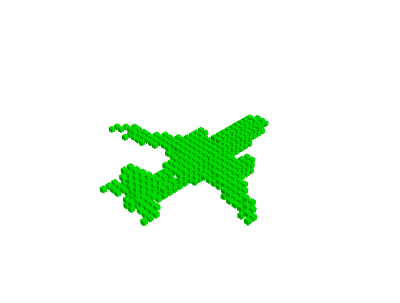
\includegraphics[width=0.19\columnwidth]{Figures/shape_retrieval/pic_airplane_30_solid.png} &
  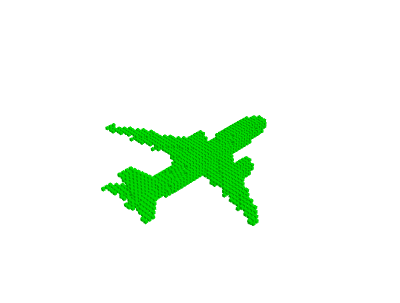
\includegraphics[width=0.19\columnwidth]{Figures/shape_retrieval/pic_airplane_50_solid.png} &
  \includegraphics[width=0.19\columnwidth]{Figures/shape_retrieval/pic_airplane_70_solid.png} &
  \includegraphics[width=0.19\columnwidth]{Figures/shape_retrieval/pic_airplane_100_solid.png} \\
% (a) first & (b) second \\
 \includegraphics[width=0.19\columnwidth]{Figures/shape_retrieval/pic_person_solid.png} &
 \includegraphics[width=0.19\columnwidth]{Figures/shape_retrieval/pic_person_30_solid.png} &
 \includegraphics[width=0.19\columnwidth]{Figures/shape_retrieval/pic_person_50_solid.png} &
 \includegraphics[width=0.19\columnwidth]{Figures/shape_retrieval/pic_person_70_solid.png} &
 \includegraphics[width=0.19\columnwidth]{Figures/shape_retrieval/pic_person_100_solid.png} \\

 \includegraphics[width=0.19\columnwidth]{Figures/shape_retrieval/pic_car_solid.png} &
 \includegraphics[width=0.19\columnwidth]{Figures/shape_retrieval/pic_car_30_solid.png} &
 \includegraphics[width=0.19\columnwidth]{Figures/shape_retrieval/pic_car_50_solid.png} &
 \includegraphics[width=0.19\columnwidth]{Figures/shape_retrieval/pic_car_70_solid.png} &
 \includegraphics[width=0.19\columnwidth]{Figures/shape_retrieval/pic_car_100_solid.png} \\
\end{tabular}
\caption{Examples of some objects voxelizations at different resolutions $30$, $50$, $70$, $100$ (from left to right), left-most objects are depicted using original meshes}
\label{fig:voxels-examples}
\end{figure}


We train Sparse 3D Convolutional Neural Network (S3DCNN) on the 3D shape classification dataset by splitting it into  training and validation subsets, adding augmentation of data to achieve rotational and translational invariance. After training a model on a dataset of pairs, we use it to embed voxel representations of 3D meshes into $192$-dimensional space. The retrieval consist of ranking search objects by a cosine distance of vectors from a query vector.

The most popular metrics for evaluating retrieval performance are
\begin{itemize}
\item Precision-Recall Curve shows a trade-off between these two measures and how quickly the precision drops with the recall increase,
\item Mean average precision (mAP). Given a query, its average precision is the average of all precision values computed on all relevant objects in the retrieved list. Given several queries, the mean average precision (mAP) is the mean of average precisions for these queries. 
\end{itemize}
We evaluated mAP for different voxel rendering sizes of 3D shapes both at train and test times, see also Figure~\ref{fig:voxels-examples}.

To check if our model is comparable with other architectures, we consider a classification task. So, we trained our model for the classification task using the ModelNet40 train subset with 
\begin{itemize}
\item SoftMax last layer for $200$ epochs,
\item with exponentially discounting learning rate,
\item and performed retrieval evaluation on the test subset,
\item taking $20$ images from every class, and ranking them w.r.t their $L2$-norm by activations taken from the $17$-th layer.
\end{itemize}

Results of these experiments are provided in Table~\ref{tab:classification}. We can see that in case of classification task setup our model is comparable in terms of the classification accuracy, but mAP values are worse. But in case of metric learning performace of S3DCNN on mAP metric is much better.
Superior performance of retrieval task with MVCNN is not a surprising result, since MVCNN uses neural nets, pre-trained on ImageNet. On the other hand our model only requires 3D Shape dataset to learn.

In Figure~\ref{fig:map_for_rs} we provide the dependence of mAP on the input spatial resolution. We can see that the retrieval performance improves with increase in the input spatial resolution up to around $45-50$, after that it drops slightly and goes to plateau. It can be attributed to the insufficient amount of layers for the same scale of features, that can be separated in higher layers. Light blue color shows range of mAP on validation for top $30$ trained architectures.


\begin{figure}[!tbp]
\vspace{-20pt}
\centering
\begin{minipage}[b]{0.45\textwidth}
  \centering
  \includegraphics[width=\columnwidth]{Figures/shape_retrieval/new_map_to_rs.pdf}
  \caption{Dependence of the retrieval performance on the input spatial resolution}
  \label{fig:map_for_rs}
\end{minipage}
\begin{minipage}[b]{0.45\textwidth}
  \centering
  \includegraphics[width=\columnwidth]{Figures/shape_retrieval/pr_curves_comp}
  \caption{Precision-Recall curve for our method}
  \label{fig:pr_curve}
\end{minipage}
\end{figure}


We would like to note that in Figure~\ref{fig:map_for_rs} mAP values provided for different validation epochs and variability of best model can be explained by difference in total learning time.

% \begin{itemize}
% \item In Table~\ref{tab:classification} for the retrieval we used features from the last but one layer of the network,
% \item In Figure~\ref{fig:map_for_rs} we used learning with the triplet loss, for which we still have to better adjust the architecture and learning rate schedule.
% \end{itemize}


\begin{figure}
\includegraphics[height=0.76\textheight]{\bilinearroot/figures/market_random.png}
\caption{The result of the proposed architecture on the Market-1501 dataset for a random subset of queries. The queries are shown on the left, and the remaining images in each row show the closest matches in the gallery dataset.}
\label{fig:market_retrieval}
\end{figure}


\section{Conclusion}
\label{sect:conclusion}

% Discuss your conclusions in order of most to least important.

In this chapter, we have compared the image-based domain adaptation techniques for face recognition in the presence of strong image degradation. We consider the recently proposed CycleGAN approach for learning mappings between the two domains of surveillance data and Internet face images. We demonstrate that the strategy of transferring the labeled Internet data to the surveillance domain and subsequent retraining the face recognition network helps to improve the recognition quality on real surveillance test data. We have investigated the variants of this approach, and have demonstrated that training on both transferred and original Internet data leads to the optimal performance. Finally, we show that in the case of our domain pair, the image-level adaptation approach outperforms feature-level domain adaptation. 

%Compare your results with those from other studies: Are they consistent? If not, discuss possible reasons for the difference.
We found our results consistent with \cite{SohnLZY0C17}, where face recognition for the low-quality is also considered. In \cite{SohnLZY0C17},  verification accuracy was improved using carefully chosen data augmentation. It is an interesting fact, that the improvement remained noticeable even when the data augmentation and the feature-level domain adaptation were applied simultaneously. Here, in contrast, we suggest performing the data augmentation in a more automatic way. Although we do not experiment with the combination of feature-level and image-level approaches to domain adaptation, we compare them independently. The combination of these adaptation techniques may further improve the results.


% Mention any inconclusive results and explain them as best you can. You may suggest additional experiments needed to clarify your results.
In our experiments, best results were achieved with training on both domains. An explanation can be given that the domain transfer model is imperfect and may push different images of the same identity too far as we do not use any kind of verification loss for training (ideally, this would require another pre-trained network for the low-quality domain, which essentially is the goal of this work). Therefore, keeping the initial data in the training set may result in less overfitting. %This can be explained by the fact that our target domain is not uniform in terms of data quality. We use two parts of the same track to generate matching pairs for each identity: e.g. these parts of each track differ in resolution (see \ref{fig:lr_hr_gan_res_ytube_initial_degraded}, columns $1$ and $3$). Therefore, using training data of diverse quality may lead to better results.  -- not true, checked.

% Briefly describe the limitations of your study to show reviewers and readers that you have considered your experiment’s weaknesses. Many researchers are hesitant to do this as they feel it highlights the weaknesses in their research to the editor and reviewer. However doing this actually makes a positive impression of your paper as it makes it clear that you have an in depth understanding of your topic and can think objectively of your research.

As an important negative result, we show that using CycleGAN-based restoration of lower-quality domain images by transferring them to the higher-quality domain does not bring consistent improvement to the recognition performance. We speculate that such transfer may distort some details of the images in a non-identity preserving way.

Our study considers a practically important domain of image data. 
We note, however, that our findings might not transfer to other pairs of domains in image adaptation.


% Discuss what your results may mean for researchers in the same field as you, researchers in other fields, and the general public. How could your findings be applied?
 
% State how your results extend the findings of previous studies.
% If your findings are preliminary, suggest future studies that need to be carried out.
% At the end of your Discussion and Conclusions sections, state your main conclusions once again.



\newpage 
\chapter{Domain-adversarial adaptation by backpropagation}
\label{chapt:gradrev}
%\section{Deep Domain Adaptation}

\def\x{{\mathbf x}}
\def\f{{\mathbf f}}

\def\S{{\cal S}}
\def\T{{\cal T}}

\def\R{{\mathds R}}

\def\tf{{\theta_f}}
\def\td{{\theta_d}}
\def\ty{{\theta_y}}
\def\htf{{\hat\theta_f}}
\def\htd{{\hat\theta_d}}
\def\hty{{\hat\theta_y}}

\subsection{The model}

We now detail the proposed model for the domain adaptation. We assume that the model works with input samples $\x \in X$, where $X$ is some input space and certain labels (output) $y$ from the label space $Y$. Below, we assume classification problems where $Y$ is a finite set ($Y=\{1,2,\dots L\}$), however our approach is generic and can handle any output label space that other deep feed-forward models can handle. We further assume that there exist two distributions $\S(x,y)$ and $\T(x,y)$ on $X\otimes Y$, which will be referred to as the source distribution and the target distribution (or the source domain and the target domain). Both distributions are assumed complex and unknown, and furthermore similar but different (in other words, $\S$ is ``shifted'' from $\T$ by some {\em domain shift}). 

Our ultimate goal is to be able to predict labels $y$ given the input $\x$ for the target distribution. At training time, we have an access to a large set of training samples $\{\x_1,\x_2,\dots,\x_N\}$ from both the source and the target domains distributed according to the marginal distributions $\S(\x)$ and $\T(\x)$. We denote with $d_i$ the binary variable ({\em domain label}) for the $i$-th example, which indicates whether $x_i$ come from the source distribution ($\x_i{\sim}\S(\x)$ if $d_i{=}0$) or from the target distribution ($\x_i{\sim}\T(\x)$ if $d_i{=}1$). For the examples from the source distribution ($d_i{=}0$) the corresponding labels $y_i \in Y$ are known at training time. For the examples from the target domains, we do not know the labels at training time, and we want to predict such labels at test time.

We now define a deep feed-forward architecture that for each input $\x$ predicts its label $y \in Y$ {\em and} its domain label $d \in \{0,1\}$. We decompose such mapping into three parts. We assume that the input $\x$ is first mapped by a mapping $G_f$ (a {\em feature extractor}) to a $D$-dimensional feature vector $\f \in \R^D$. The feature mapping may also include several feed-forward layers and we denote the vector of parameters of all layers in this mapping as $\tf$, i.e.\ $\f = G_f(\x;\tf)$. Then, the feature vector $\f$ is mapped by a mapping $G_y$ ({\em label predictor}) to the label $y$, and we denote the parameters of this mapping with $\ty$. Finally, the same feature vector $\f$ is mapped to the domain label $d$ by a mapping $G_d$ ({\em domain classifier}) with the parameters $\td$ (\fig{arch}).

During the learning stage, we aim to minimize the label prediction loss on the annotated part (i.e.\ the source part) of the training set, and the parameters of both the feature extractor and the label predictor are thus optimized in order to minimize the empirical loss for the source domain samples. This ensures the discriminativeness of the features $\f$ and the overall good prediction performance of the combination of the feature extractor and the label predictor on the source domain.

At the same time, we want to make the features $\f$ domain-invariant. That is, we want to make the distributions $S(\f) = \{G_f(\x; \tf)\,|\, \x{\sim}S(\x)\}$ and $T(\f) = \{G_f(\x; \tf)\,|\, \x{\sim}T(\x)\}$ to be similar. Under the {\em covariate shift} assumption, this would make the label prediction accuracy on the target domain to be the same as on the source domain~\cite{Shimodaira00}. Measuring the dissimilarity of the distributions $S(\f)$ and $T(\f)$ is however non-trivial, given that $\f$ is high-dimensional, and that the distributions themselves are constantly changing as learning progresses. One way to estimate the dissimilarity is to look at the loss of the domain classifier $G_d$, provided that the parameters $\td$ of the domain classifier have been trained to discriminate between the two feature distributions in an optimal way. 

This observation leads to our idea. At training time, in order to obtain domain-invariant features, we seek the parameters $\tf$ of the feature mapping that {\em maximize} the loss of the domain classifier (by making the two feature distributions as similar as possible), while simultaneously seeking the parameters $\td$ of the domain classifier that {\em minimize} the loss of the domain classifier. In addition, we seek to minimize the loss of the label predictor. 

More formally, we consider the functional:
\begin{gather} 
E(\tf,\ty,\td) =  \sum_{\substack{i=1..N\\d_i = 0}} L_y\left( \strut G_y(G_f(\x_i;\tf);\ty), y_i\right) -\nonumber\\ \lambda \sum_{i=1..N} L_d \left( \strut G_d(G_f(\x_i;\tf);\td), y_i\right) = \nonumber\\= \sum_{\substack{i=1..N\\d_i = 0}} L^i_y( \tf, \ty) - \lambda \sum_{i=1..N} L^i_d( \tf, \td) 
\label{eq:func}
\end{gather}
Here, $L_y(\cdot,\cdot)$ is the loss for label prediction (e.g.\ multinomial), $L_d(\cdot,\cdot)$ is the loss for the domain classification (e.g.\ logistic), while $L^i_y$ and $L^i_d$ denote the corresponding loss functions evaluated at the $i$-th training example. 

Based on our idea, we are seeking the parameters $\htf,\hty,\htd$ that deliver a saddle point of the functional \eq{func}:

\begin{gather}
(\htf,\hty) = \arg\min_{\tf,\ty} E(\tf,\ty,\htd)\,\label{eq:opt1}\\\label{eq:opt2}
\htd = \arg\max_\td E(\htf,\hty, \td)\,.
\end{gather}

At the saddle point, the parameters $\td$ of the domain classifier $\td$ minimize the domain classification loss (since it enters into \eq{func} with the minus sign) while the parameters $\ty$ of the label predictor minimize the label prediction loss. The feature mapping parameters $\tf$ {\em minimize} the label prediction loss (i.e.\ the features are discriminative), while {\em maximizing} the domain classification loss (i.e.\ the features are domain-invariant). The parameter $\lambda$ controls the trade-off between the two objectives that shape the features during learning.

Below, we demonstrate that standard stochastic gradient solvers (SGD) can be adapted for the search of the saddle point \eq{opt1}-\eq{opt2}.

\subsection{Optimization with backpropagation}

A saddle point \eq{opt1}-\eq{opt2} can be found as a stationary point of the following stochastic updates:

\begin{align}
\tf \quad &\longleftarrow \quad \tf \;-\; \mu \left(\frac{\partial L^i_y}{\partial \tf}-\lambda\frac{\partial L^i_d}{\partial \tf} \right) \label{eq:upd1}\\
\ty \quad &\longleftarrow \qquad \ty \;-\; \mu \frac{\partial L^i_y}{\partial \ty}\label{eq:upd2}\\
\td \quad &\longleftarrow \qquad \td \;-\; \mu \frac{\partial L^i_d}{\partial \td} \label{eq:upd3}
\end{align}
where $\mu$ is the learning rate (which can vary over time).

The updates \eq{upd1}-\eq{upd3} are very similar to stochastic gradient descent (SGD) updates for a feed-forward deep model that comprises feature extractor fed into the label predictor and into the domain classifier. The difference is the $-\lambda$ factor in \eq{upd1} (the difference is important, as without such factor, stochastic gradient descent would try to make features dissimilar across domains in order to minimize the domain classification loss). Although direct implementation of \eq{upd1}-\eq{upd3} as SGD is not possible, it is highly desirable to reduce the updates \eq{upd1}-\eq{upd3} to some form of SGD, since SGD (and its variants) is the main learning algorithm implemented in most packages for deep learning. 

Fortunately, such reduction can be accomplished by introducing a special {\bf gradient reversal layer} (GRL) defined as follows. The gradient reversal layer has no parameters associated with it (apart from the meta-parameter $\lambda$, which is not updated by backpropagation). During the forward propagation, GRL acts as an identity transform. During the backpropagation though, GRL takes the gradient from the subsequent level, multiplies it by $-\lambda$ and passes it to the preceding layer. Implementing such layer using existing object-oriented packages for deep learning is simple, as defining procedures for forwardprop (identity transform), backprop (multiplying by a constant), and parameter update (nothing) is trivial. 

The GRL as defined above is inserted between the feature extractor and the domain classifier, resulting in the architecture depicted in \fig{arch}. As the backpropagation process passes through the GRL, the partial derivatives of the loss that is downstream the GRL (i.e.\ $L_d$) w.r.t.\ the layer parameters that are upstream the GRL (i.e.\ $\tf$) get multiplied by $-\lambda$, i.e.\ $\frac{\partial L_d}{\partial \tf}$ is effectively replaced with $-\lambda\frac{\partial L_d}{\partial \tf}$. Therefore, running SGD in the resulting model implements the updates \eq{upd1}-\eq{upd3} and converges to a saddle point of \eq{func}.

Mathematically, we can formally treat the gradient reversal layer as a ``pseudo-function'' $R_\lambda(\x)$ defined by two (incompatible) equations describing its forward- and backpropagation behaviour:
\begin{align}
R_\lambda(\x) = \x\\
\frac{dR_\lambda}{d\x} = -\lambda \mathbf{I}
\end{align}
where $\mathbf{I}$ is an identity matrix.
We can then define the objective ``pseudo-function'' of $(\tf,\ty,\td)$ that is being optimized by the stochastic gradient descent within our method:
\begin{gather}
\tilde E(\tf,\ty,\td) =  \sum_{\substack{i=1..N\\d_i = 0}} L_y\left( \strut G_y(G_f(\x_i;\tf);\ty), y_i\right) +\nonumber\\ \sum_{i=1..N} L_d \left( \strut G_d(R_\lambda(G_f(\x_i;\tf));\td), y_i\right) \label{eq:pseudoobj}
\end{gather}

Running updates \eq{upd1}-\eq{upd3} can then be implemented as doing SGD for \eq{pseudoobj} and leads to the emergence of features that are domain-invariant and discriminative at the same time. After the learning, the label predictor $y(\x) = G_y(G_f(\x;\tf);\ty)$ can be used to predict labels for samples from the target domain (as well as from the source domain).

The simple learning procedure outlined above can be re-derived/generalized along the lines suggested in \cite{Goodfellow14} (see \cite{SuppMat}).

% \subsection{Relation to $ \mathcal{H} \Delta \mathcal{H} $-distance}
% \label{sect:theory}

% In this section we give a brief analysis of our method in terms of $ \mathcal{H} \Delta \mathcal{H} $-distance \cite{Ben10,Cortes11} which is widely used in the theory of non-conservative domain adaptation. Formally,
% \begin{multline}
%   d_{\mathcal{H} \Delta \mathcal{H}} (\mathcal{S}, \mathcal{T}) = 2 \sup_{h_1, h_2 \in \mathcal{H}} \left| P_{\mathbf{f} \sim \mathcal{S}} [h_1(\mathbf{f}) \neq h_2(\mathbf{f})] - \right. \\
%   \left. - P_{\mathbf{f} \sim \mathcal{T}} [h_1(\mathbf{f}) \neq h_2(\mathbf{f})] \right|
% \label{eq:hdh_dist}
% \end{multline}
% defines a discrepancy distance between two distributions $ \mathcal{S} $ and $ \mathcal{T} $ w.r.t. a hypothesis set $ \mathcal{H} $. Using this notion one can obtain a probabilistic bound \cite{Ben10} on the performance $ \varepsilon_\mathcal{T}(h) $ of some classifier $ h $ from $ \mathcal{T} $ evaluated on the target domain given its performance $ \varepsilon_\mathcal{S}(h) $ on the source domain:
% \begin{equation}
%   \varepsilon_\mathcal{T}(h) \leq \varepsilon_\mathcal{S}(h) + \frac{1}{2} d_{\mathcal{H} \Delta \mathcal{H}} (\mathcal{S}, \mathcal{T}) + C \, ,
% \end{equation}
% where $ \mathcal{S} $ and $ \mathcal{T} $ are source and target distributions respectively, and $ C $ does not depend on particular $ h $. 

% Consider fixed $ \mathcal{S} $ and $ \mathcal{T} $ over the representation space produced by the feature extractor $ G_f $ and a family of label predictors $ \mathcal{H}_p $. We assume that the family of domain classifiers $ \mathcal{H}_d $ is rich enough to contain the symmetric difference hypothesis set of $ \mathcal{H}_p $:
% \begin{equation}
%   \mathcal{H}_p \Delta \mathcal{H}_p = \left\{ h \, | \, h = h_1 \oplus h_2 \, , \; h_1, h_2 \in \mathcal {H}_p \right\} \, .
% \end{equation}
% It is not an unrealistic assumption as we have a freedom to pick $ \mathcal{H}_d $ whichever we want. For example, we can set the architecture of the domain discriminator to be the layer-by-layer concatenation of two replicas of the label predictor followed by a two layer non-linear perceptron aimed to learn the \texttt{XOR}-function. Given the assumption holds, one can easily show that training the $ G_d $ is closely related to the estimation of $ d_{\mathcal{H}_p \Delta \mathcal{H}_p} (\mathcal{S}, \mathcal{T}) $. Indeed, 
% \begin{equation}
% \begin{split}
%   &d_{\mathcal{H}_p \Delta \mathcal{H}_p}  (\mathcal{S}, \mathcal{T}) =\\ 
%   & = 2 \sup_{h \in \mathcal{H}_p \Delta \mathcal{H}_p} \left| P_{\mathbf{f} \sim \mathcal{S}} [h(\mathbf{f}) = 1] - P_{\mathbf{f} \sim \mathcal{T}} [h(\mathbf{f}) = 1] \right| \leq \\
%   & \leq 2 \sup_{h \in \mathcal{H}_d} \left| P_{\mathbf{f} \sim \mathcal{S}} [h(\mathbf{f}) = 1] - P_{\mathbf{f} \sim \mathcal{T}} [h(\mathbf{f}) = 1] \right| = \\
%   & = 2 \sup_{h \in \mathcal{H}_d} \left| 1 - \alpha(h) \right| = 2 \sup_{h \in \mathcal{H}_d} \left[ \alpha(h) - 1 \right]
% \end{split}
% \end{equation}
% where $ \alpha(h) = P_{\mathbf{f} \sim \mathcal{S}} [h(\mathbf{f}) = 0] + P_{\mathbf{f} \sim \mathcal{T}} [h(\mathbf{f}) = 1] $ is maximized by the optimal $ G_d $.

% Thus, optimal discriminator gives the upper bound for $ d_{\mathcal{H}_p \Delta \mathcal{H}_p}  (\mathcal{S}, \mathcal{T}) $. At the same time, backpropagation of the reversed gradient changes the representation space so that $ \alpha(G_d) $ becomes smaller effectively reducing $ d_{\mathcal{H}_p \Delta \mathcal{H}_p}  (\mathcal{S}, \mathcal{T}) $ and leading to the better approximation of $ \varepsilon_\mathcal{T}(G_y) $ by $ \varepsilon_\mathcal{S}(G_y) $.

%
\subsection{Experiments with Deep Image Descriptors for Re-Identification}

% In this section we discuss the application of the described adaptation method to person re-identification \textit{(re-id}) problem.  The task of person re-identification is to associate people seen from different camera views. More formally, it can be defined as follows: given two sets of images from different cameras (\textit{probe} and \textit{gallery}) such that each person depicted in the probe set has an image in the gallery set,  for each image of a person from the probe set find an image of the same person in the gallery set.  Disjoint camera views, different illumination conditions, various poses and low quality of data make this problem difficult  even for humans (\eg, \citet{LiuLGW13} reports human performance at Rank1=$71.08\%$).  

% Unlike classification problems that are discussed above, re-identification problem implies that each image is mapped to a vector descriptor. The distance between descriptors is then used to match images from the probe set and the gallery set.
% To evaluate results of re-id methods the \textit{Cumulative Match Characteristic} (CMC) curve is commonly used. It is a plot of the identification rate (recall) at rank-$k$, that is the probability of the matching gallery image to be within the closest $k$ images (in terms of descriptor distance) to the probe image.

% Most existing works train descriptor mappings and evaluate them within the same data set containing images from a certain camera network with similar imaging conditions. Several papers, however, observed that the performance of the resulting re-identification systems drops very considerably when descriptors trained on one data set and tested on another. It is therefore natural to handle such cross-domain evaluation as a domain-adaptation problem, where each camera network (data set) constitutes a domain.

% Recently, several papers  with significantly improved re-identification performance \citep{ZhangS14a,ZhaoOW14,Paisitkriangkrai15} have been presented, with \citet{MaLYL15} reporting good results in cross-data-set evaluation scenario. At the moment, deep learning methods \citep{YiLL14} do not achieve state-of-the-art results probably because of the limited size of the training sets. Domain adaptation thus represents a viable direction for improving deep re-identification descriptors.

% \subsubsection{Data Sets and Protocols} 

% Following \citet{MaLYL15}, we use PRID \citep{Hirzer_h.:person}, VIPeR \citep{Gray07evaluatingappearance}, CUHK \citep{LiW13} as target data sets for our experiments.  

%------------------------to main intro------------
%The \textit{PRID} data set exists in two versions, and as in \citep{MaLYL15} we use a single-shot variant. It contains images of $385$ persons viewed from camera A and images of $749$ persons viewed from camera B,  $200$ persons appear in both cameras. The \textit{VIPeR} data set also contains images taken with two cameras, and in total $632$ persons are captured, for every person there is one image for each of the two camera views. The \textit{CUHK} data set consists of images from five pairs of cameras, two images for each person from each of the two cameras. We refer to the subset of this data set that includes the first pair of cameras only as \textit{CUHK/p1} (as most papers use this subset).

% We perform extensive experiments for various pairs of data sets, where one data set serves as a source domain, \ie, it is used to train a descriptor mapping in a supervised way with known correspondences between probe and gallery images. The second data set is used as a target domain, so that images from that data set are used without probe-gallery correspondence.

% In more detail, CUHK/p1 is used for experiments when CUHK serves as a target domain and two settings (``whole CUHK'' and CUHK/p1) are used for experiments when CUHK serves as a source domain. Given PRID as a target data set, we randomly choose 100 persons appearing in both camera views as training set. The images of the other 100 persons from camera A are used as probe, all images from camera B excluding those used in training (649 in total) are used as gallery at test time. For VIPeR, we use random 316 persons for training and all others for testing. For CUHK, 971 persons are split into 485 for training and 486 for testing.
% Unlike \citet{MaLYL15}, we use all images in the first  pair of cameras of CUHK instead of choosing one image of a person from each camera view. We also performed two experiments with all images of the whole CUHK data set as source domain and VIPeR and PRID data sets as target domains as in the  original paper \citep{YiLL14}.
------------------
\newlength\reidheight
\setlength{\reidheight}{2.5cm}

\addtolength{\tabcolsep}{-3pt}

\begin{figure*}
\centering
\begin{tabular}{cccc|cccc|cccc}
\includegraphics[height=\reidheight]{Chapters/gradrev/figures/dataset_samples/viper/a/000_45.png}&
\includegraphics[height=\reidheight]{Chapters/gradrev/figures/dataset_samples/viper/b/000_45.png}&
\includegraphics[height=\reidheight]{Chapters/gradrev/figures/dataset_samples/viper/a/001_45.png}&
\includegraphics[height=\reidheight]{Chapters/gradrev/figures/dataset_samples/viper/b/002_90.png}&
\includegraphics[height=\reidheight]{Chapters/gradrev/figures/dataset_samples/PRID/a/img_0001.png}&
\includegraphics[height=\reidheight]{Chapters/gradrev/figures/dataset_samples/PRID/b/img_0001.png}&
\includegraphics[height=\reidheight]{Chapters/gradrev/figures/dataset_samples/PRID/a/img_0002.png}&
\includegraphics[height=\reidheight]{Chapters/gradrev/figures/dataset_samples/PRID/b/img_0003.png}&
\includegraphics[height=\reidheight]{Chapters/gradrev/figures/dataset_samples/cuhk/a/001_00005.png}&
\includegraphics[height=\reidheight]{Chapters/gradrev/figures/dataset_samples/cuhk/b/001_00221.png}&
\includegraphics[height=\reidheight]{Chapters/gradrev/figures/dataset_samples/cuhk/a/002_00280.png}&
\includegraphics[height=\reidheight]{Chapters/gradrev/figures/dataset_samples/cuhk/b/003_00403.png}\\
\multicolumn{4}{c}{VIPER}&
\multicolumn{4}{c}{PRID}&
\multicolumn{4}{c}{CUHK}
\end{tabular}
\caption{Matching and non-matching pairs of probe-gallery images from different person re-identification data sets. The three data sets are treated as different domains in our experiments.}
\label{fig:reidsamples}
\end{figure*}

\addtolength{\tabcolsep}{3pt}

Following \citet{YiLL14}, we augmented our data with mirror images, and during test time we calculate similarity score between two images as the mean of the four scores corresponding to different flips of the two compared images. In case of CUHK, where there are 4 images (including mirror images) for each of the two camera views for each person, all 16 combinations' scores are averaged. 

\subsubsection{CNN architectures and Training Procedure} 

In our experiments, we use siamese architecture described in \citet{YiLL14} (\textit{Deep Metric Learning} or \textit{DML}) for learning deep image descriptors on the source data set.
This architecture incorporates two convolution layers (with $7\times7$ and $5\times5$ filter banks), followed by ReLU and max pooling, and one fully-connected layer, which gives $500$-dimensional descriptors as an output. There are three parallel flows within the CNN for processing three part of an image: the upper, the middle, and the lower one. The first convolution layer shares parameters between three parts, and the outputs of the second convolution layers are concatenated.
During training, we follow \citet{YiLL14} and calculate pairwise cosine similarities between $500$-dimensional features within each batch and backpropagate the loss for all pairs within batch. 

To perform domain-adversarial training, we construct a DANN architecture.  The feature extractor includes the two convolutional layers (followed by max-pooling and ReLU) discussed above. The label predictor in this case is replaced with \textit{descriptor predictor} that includes one fully-connected layer. The domain classifier includes two fully-connected layers with $500$ units in the intermediate representation ($x{\rightarrow}500{\rightarrow}1$). 

For the verification loss function in the descriptor predictor we used Binomial Deviance loss, defined in \citet{YiLL14} with similar parameters: $\alpha = 2$, $\beta = 0.5$, $c = 2$ (the asymmetric cost parameter for negative pairs). The domain classifier is trained with logistic loss as in subsection  \ref{train_proc_for_classification}.

We used learning rate fixed to $0.001$ and momentum of $0.9$. The schedule of adaptation similar to the one described in subsection \ref{train_proc_for_classification} was used. We also inserted dropout layer with rate $0.5$ after the concatenation of outputs of the second max-pooling layer. $128$-sized batches were used for source data and $128$-sized batches for target data. 

%TODO fix 
% \begin{figure*}[t]
%   \definecolor{fnodebottom}{RGB}{132,170,81}
%   \definecolor{fnodetop}{RGB}{172,222,106}
%   \definecolor{cnodebottom}{RGB}{120,128,164}
%   \definecolor{cnodetop}{RGB}{158,167,218}
%   \definecolor{dnodebottom}{RGB}{174,109,146}
%   \definecolor{dnodetop}{RGB}{230,141,192}
%   \centering
%   {%
%      \scalebox{0.65}{\input{./Chapters/gradrev/figures/archs/reidentification_adaptation.tikz}}}\\
%   \caption{CNN architecture used in experiments on domain adaptation for person re-identification}
%   \label{fig:reid_arch}
% \end{figure*}

\subsubsection{Results on Re-identification data sets} 

\begin{figure}[t]
\centering
  \begin{tabular}{p{5cm}  p{5cm}  p{5cm} }
      
        \setlength\figureheight{3.5cm}
        \setlength\figurewidth{3.5cm}
        \begin{tikzpicture}[font=\scriptsize]

\begin{axis}[%
width=0.95092\figurewidth,
height=\figureheight,
at={(0\figurewidth,0\figureheight)},
scale only axis,
xmin=1,
xmax=50,
xlabel={Rank},
ymin=0,
ymax=1,
ylabel={Identification rate (\%)},
axis x line*=bottom,
axis y line*=left,
legend style={at={($ (0,1) + (+0.1cm,+0.1cm) $)},anchor=north west,align=left,legend cell align=left,draw=black},
xmajorgrids,
ymajorgrids,
grid style={dashed}
]
\addplot [color=blue,solid,line width=1.0pt]
  table[row sep=crcr]{%
1    0.1518987341772152\\
5    0.34810126582278483\\
10   0.47468354430379744\\
15   0.5474683544303798\\
20   0.5886075949367089\\
25   0.629746835443038\\
30   0.6613924050632911\\
35   0.680379746835443\\
40   0.7120253164556962\\
45   0.7183544303797469\\
50   0.7310126582278481\\
};
\addlegendentry{DML};

\addplot [color=cyan,solid,line width=1.0pt]
  table[row sep=crcr]{%
1    0.14556962025316456\\
5    0.3322784810126582\\
10   0.4873417721518987\\
15   0.5569620253164557\\
20   0.5917721518987342\\
25   0.6424050632911392\\
30   0.689873417721519\\
35   0.7025316455696202\\
40   0.7278481012658228\\
45   0.7531645569620253\\
50   0.7848101265822784\\
};
\addlegendentry{DML, adaptation};



\end{axis}
\end{tikzpicture}%
        \centering\small{(a) Whole CUHK $\rightarrow$ VIPeR}
        \label{fig:allcuhk_viper}
  
    &
        \setlength\figureheight{3.5cm}
        \setlength\figurewidth{3.5cm}
        \begin{tikzpicture}[font=\scriptsize]

\begin{axis}[%
width=0.95092\figurewidth,
height=\figureheight,
at={(0\figurewidth,0\figureheight)},
scale only axis,
xmin=1,
xmax=50,
xlabel={Rank},
ymin=0,
ymax=1,
ylabel={Identification rate (\%)},
axis x line*=bottom,
axis y line*=left,
legend style={at={($ (0,1) + (+0.1cm,+0.1cm) $)},anchor=north west,align=left,legend cell align=left,draw=black},
xmajorgrids,
ymajorgrids,
grid style={dashed}
]
\addplot [color=blue,solid,line width=1.0pt]
  table[row sep=crcr]{%
1      0.126582278481 \\
5      0.303797468354 \\
10      0.414556962025 \\
15      0.490506329114 \\
20      0.550632911392 \\
25      0.613924050633 \\
30      0.651898734177 \\
35      0.686708860759 \\
40      0.708860759494 \\
45      0.75 \\
50      0.759493670886 \\
};
\addlegendentry{DML};

\addplot [color=cyan,solid,line width=1.0pt]
  table[row sep=crcr]{%
1      0.120253164557 \\
5      0.29746835443 \\
10      0.462025316456 \\
15      0.541139240506 \\
20      0.594936708861 \\
25      0.617088607595 \\
30      0.645569620253 \\
35      0.667721518987 \\
40      0.696202531646 \\
45      0.712025316456 \\
50      0.73417721519 \\
};
\addlegendentry{DML, adaptation};


\end{axis}
\end{tikzpicture}%
        \centering\small{(b) CUHK/p1 $\rightarrow$ VIPeR}
%        \label{fig:cuhk_p1_viper}
    &
        \setlength\figureheight{3.5cm}
        \setlength\figurewidth{3.5cm}
        \begin{tikzpicture}[font=\scriptsize]

\begin{axis}[%
width=0.95092\figurewidth,
height=\figureheight,
at={(0\figurewidth,0\figureheight)},
scale only axis,
xmin=1,
xmax=50,
xlabel={Rank},
ymin=0,
ymax=1,
ylabel={Identification rate (\%)},
axis x line*=bottom,
axis y line*=left,
legend style={at={($ (0,1) + (+0.1cm,+0.1cm) $)},anchor=north west,align=left,legend cell align=left,draw=black},
xmajorgrids,
ymajorgrids,
grid style={dashed}
]
\addplot [color=blue,solid,line width=1.0pt]
  table[row sep=crcr]{%
1      0.0664556962025 \\
5      0.167721518987 \\
10      0.253164556962 \\
15      0.275316455696 \\
20      0.316455696203 \\
25      0.348101265823 \\
30      0.379746835443 \\
35      0.414556962025 \\
40      0.45253164557 \\
45      0.474683544304 \\
50      0.496835443038 \\
};
\addlegendentry{DML};

\addplot [color=cyan,solid,line width=1.0pt]
  table[row sep=crcr]{%
1      0.0632911392405 \\
5      0.161392405063 \\
10      0.259493670886 \\
15      0.338607594937 \\
20      0.389240506329 \\
25      0.417721518987 \\
30      0.439873417722 \\
35      0.471518987342 \\
40      0.496835443038 \\
45      0.518987341772 \\
50      0.53164556962 \\
};
\addlegendentry{DML, adaptation};


\end{axis}
\end{tikzpicture}%
        \centering\small{(c) PRID $\rightarrow$ VIPeR}
%        \label{fig:cuhk_p1_viper} \\    
 \end{tabular}
%  \caption{Results on VIPeR}
%  \label{fig:viper}
% \end{figure}%

% \begin{figure}[h]
% \centering
 \begin{tabular}{ p{5cm}  p{5cm}  p{5cm} }
        \setlength\figureheight{3.5cm}
        \setlength\figurewidth{4cm}
        \begin{tikzpicture}[font=\scriptsize]

\begin{axis}[%
width=0.95092\figurewidth,
height=\figureheight,
at={(0\figurewidth,0\figureheight)},
scale only axis,
xmin=1,
xmax=50,
xlabel={Rank},
ymin=0,
ymax=1,
ylabel={Identification rate (\%)},
axis x line*=bottom,
axis y line*=left,
legend style={at={($ (0,1) + (+0.1cm,+0.1cm) $)},anchor=north west,align=left,legend cell align=left,draw=black},
xmajorgrids,
ymajorgrids,
grid style={dashed}
]
\addplot [color=blue,solid,line width=1.0pt]
  table[row sep=crcr]{%
1    0.08\\
5    0.13\\
10   0.22\\
15   0.27\\
20   0.31\\
25   0.35\\
30   0.4\\
35   0.41\\
40   0.41\\
45   0.43\\
50   0.44\\
};
\addlegendentry{DML};

\addplot [color=cyan,solid,line width=1.0pt]
  table[row sep=crcr]{%
1    0.07\\
5    0.19\\
10   0.27\\
15   0.32\\
20   0.35\\
25   0.37\\
30   0.39\\
35   0.41\\
40   0.43\\
45   0.45\\
50   0.45\\
};
\addlegendentry{DML, adaptation};


%[0.08, 0.13, 0.22, 0.27, 0.31, 0.35, 0.4, 0.41, 0.41, 0.43, 0.44]
%[0.07, 0.19, 0.27, 0.32, 0.35, 0.37, 0.39, 0.41, 0.43, 0.45, 0.45]

%
\end{axis}
\end{tikzpicture}%





        \centering\small{(d) Whole CUHK $\rightarrow$ PRID}
        \label{fig:allcuhk_prid}
    &
        \setlength\figureheight{3.5cm}
        \setlength\figurewidth{4cm}
        \begin{tikzpicture}[font=\scriptsize]

\begin{axis}[%
width=0.95092\figurewidth,
height=\figureheight,
at={(0\figurewidth,0\figureheight)},
scale only axis,
xmin=1,
xmax=50,
xlabel={Rank},
ymin=0,
ymax=1,
ylabel={Identification rate (\%)},
axis x line*=bottom,
axis y line*=left,
legend style={at={($ (0,1) + (+0.1cm,+0.1cm) $)},anchor=north west,align=left,legend cell align=left,draw=black},
xmajorgrids,
ymajorgrids,
grid style={dashed}
]
\addplot [color=blue,solid,line width=1.0pt]
  table[row sep=crcr]{%
1      0.04 \\
5      0.08 \\
10      0.15 \\
15      0.22 \\
20      0.25 \\
25      0.3 \\
30      0.32 \\
35      0.36 \\
40      0.39 \\
45      0.41 \\
50      0.44 \\
};
\addlegendentry{DML};

\addplot [color=cyan,solid,line width=1.0pt]
  table[row sep=crcr]{%
1      0.06 \\
5      0.16 \\
10      0.21 \\
15      0.27 \\
20      0.31 \\
25      0.36 \\
30      0.39 \\
35      0.41 \\
40      0.41 \\
45      0.42 \\
50      0.43 \\
};
\addlegendentry{DML, adaptation};


\end{axis}
\end{tikzpicture}%
        \centering\small{(e) CUHK/p1 $\rightarrow$ PRID}
        \label{fig:cuhk_p1_prid}
    &
       \setlength\figureheight{3.5cm}
       \setlength\figurewidth{4cm}
       \begin{tikzpicture}[font=\scriptsize]

\begin{axis}[%
width=0.95092\figurewidth,
height=\figureheight,
at={(0\figurewidth,0\figureheight)},
scale only axis,
xmin=1,
xmax=50,
xlabel={Rank},
ymin=0,
ymax=1,
ylabel={Identification rate (\%)},
axis x line*=bottom,
axis y line*=left,
legend style={at={($ (0,1) + (+0.1cm,+0.1cm) $)},anchor=north west,align=left,legend cell align=left,draw=black},
xmajorgrids,
ymajorgrids,
grid style={dashed}
]
\addplot [color=blue,solid,line width=1.0pt]
  table[row sep=crcr]{%
1      0.08 \\
5      0.15 \\
10      0.19 \\
15      0.25 \\
20      0.28 \\
25      0.34 \\
30      0.35 \\
35      0.36 \\
40      0.39 \\
45      0.4 \\
50      0.41 \\
};
\addlegendentry{DML};

\addplot [color=cyan,solid,line width=1.0pt]
  table[row sep=crcr]{%
1      0.07 \\
5      0.19 \\
10      0.25 \\
15      0.27 \\
20      0.31 \\
25      0.36 \\
30      0.39 \\
35      0.42 \\
40      0.42 \\
45      0.46 \\
50      0.47 \\
};
\addlegendentry{DML, adaptation};


\end{axis}
\end{tikzpicture}%
        \centering\small{(f) VIPeR $\rightarrow$ PRID}
        \label{fig:viper_prid}  \\    
 \end{tabular}
%  \caption{Results on PRID}
%  \label{fig:prid}
% \end{figure}


% \begin{figure}[h]
% \centering
 \begin{tabular}{ p{5cm}  p{5cm}}
        \setlength\figureheight{3.5cm}
        \setlength\figurewidth{4cm}
        \begin{tikzpicture}[font=\scriptsize]

\begin{axis}[%
width=0.95092\figurewidth,
height=\figureheight,
at={(0\figurewidth,0\figureheight)},
scale only axis,
xmin=1,
xmax=50,
xlabel={Rank},
ymin=0,
ymax=1,
ylabel={Identification rate (\%)},
axis x line*=bottom,
axis y line*=left,
legend style={at={($ (0,1) + (+0.1cm,+0.1cm) $)},anchor=north west,align=left,legend cell align=left,draw=black},
xmajorgrids,
ymajorgrids,
grid style={dashed}
]
\addplot [color=blue,solid,line width=1.0pt]
  table[row sep=crcr]{%
1      0.109053497942 \\
5      0.265432098765 \\
10      0.366255144033 \\
15      0.407407407407 \\
20      0.465020576132 \\
25      0.491769547325 \\
30      0.510288065844 \\
35      0.541152263374 \\
40      0.572016460905 \\
45      0.59670781893 \\
50      0.617283950617 \\
};
\addlegendentry{DML};

\addplot [color=cyan,solid,line width=1.0pt]
  table[row sep=crcr]{%
1      0.125514403292 \\
5      0.253086419753 \\
10      0.366255144033 \\
15      0.440329218107 \\
20      0.5 \\
25      0.5329218107 \\
30      0.572016460905 \\
35      0.594650205761 \\
40      0.617283950617 \\
45      0.650205761317 \\
50      0.668724279835 \\
};
\addlegendentry{DML, adaptation};


\end{axis}
\end{tikzpicture}%
        \centering\small{(g) VIPeR $\rightarrow$ CUHK/p1}
        \label{fig:viper_cuhk_p1}
    &
        \setlength\figureheight{3.5cm}
        \setlength\figurewidth{4cm}
        \begin{tikzpicture}[font=\scriptsize]

\begin{axis}[%
width=0.95092\figurewidth,
height=\figureheight,
at={(0\figurewidth,0\figureheight)},
scale only axis,
xmin=1,
xmax=50,
xlabel={Rank},
ymin=0,
ymax=1,
ylabel={Identification rate (\%)},
axis x line*=bottom,
axis y line*=left,
legend style={at={($ (0,1) + (+0.1cm,+0.1cm) $)},anchor=north west,align=left,legend cell align=left,draw=black},
xmajorgrids,
ymajorgrids,
grid style={dashed}
]
\addplot [color=blue,solid,line width=1.0pt]
  table[row sep=crcr]{%
1      0.0569620253165 \\
5      0.139240506329 \\
10      0.212025316456 \\
15      0.284810126582 \\
20      0.316455696203 \\
25      0.344936708861 \\
30      0.370253164557 \\
35      0.389240506329 \\
40      0.414556962025 \\
45      0.443037974684 \\
50      0.465189873418 \\
};
\addlegendentry{DML};

\addplot [color=cyan,solid,line width=1.0pt]
  table[row sep=crcr]{%
1      0.0843621399177 \\
5      0.191358024691 \\
10      0.263374485597 \\
15      0.316872427984 \\
20      0.347736625514 \\
25      0.395061728395 \\
30      0.432098765432 \\
35      0.471193415638 \\
40      0.504115226337 \\
45      0.5329218107 \\
50      0.553497942387 \\
};
\addlegendentry{DML, adaptation};


\end{axis}
\end{tikzpicture}%
        \centering\small{(h) PRID $\rightarrow$ CUHK/p1}
        \label{fig:prid_cuhk_p1}
  \\    
  \end{tabular}
  \caption{Results on VIPeR, PRID and CUHK/p1 with and without domain-adversarial learning. Across the eight domain pairs domain-adversarial learning improves re-identification accuracy. For some domain pairs the improvement is considerable.}
  \label{fig:adaptresults}
\end{figure}

Figure \ref{fig:adaptresults} shows results in the form of CMC-curves for eight pairs of data sets. Depending on the hardness of the annotation problem we trained either for 50,000 iterations (CUHK/p1 $\rightarrow$ VIPeR, VIPeR $\rightarrow$ CUHK/p1, PRID $\rightarrow$ VIPeR) or for 20,000 iterations (the other five pairs). 

\begin{figure*}
\centering
\begin{tabular}{c c}
\includegraphics[height=7cm, width=7cm]{./Chapters/gradrev/figures/reid_adapt_results/viper_cuhkp1_zc.png}&
\includegraphics[height=7cm, width=7cm]{./Chapters/gradrev/figures/reid_adapt_results/viper_cuhkp1_da.png}\\
\small{(a) DML}&
\small{(b) DML, adaptation}\\
\end{tabular}
\caption{The effect of adaptation shown by t-SNE visualizations of source and target domains descriptors in a VIPeR $\rightarrow$ CUHK/p1 experiment pair. VIPeR is depicted with \textit{green} and CUHK/p1 - with \textit{red}. As in the image classification case, domain-adversarial learning ensures a closer match between the source and the target distributions. }
\label{fig:reidtsne}
\end{figure*}


After the sufficient number of iterations, domain-adversarial training consistently improves the performance of re-identification. For the pairs that involve PRID data set, which is more dissimilar to the other two data sets, the improvement is considerable. Overall, this demonstrates the applicability of the domain-adversarial learning beyond classification problems.

Figure \ref{fig:reidtsne} further demonstrates the effect of adaptation on the distributions of the learned descriptors in the source and in target sets in VIPeR $\rightarrow$ CUHK/p1 experiments, where domain adversarial learning once again achieves better intermixing of the two domains.


\section{Conclusion}

The paper proposes a new approach to domain adaptation of feed-forward neural networks, which allows large-scale training based on large amount of annotated data in the source domain and large amount of unannotated data in the target domain. Similarly to many previous shallow and deep DA techniques, the adaptation is achieved through aligning the distributions of features across the two domains. However, unlike previous approaches, the alignment is accomplished through standard backpropagation training.

The approach is motivated and supported by the domain adaptation theory of \citet{BenDavid-NIPS06,BenDavid-MLJ2010}. 
The main idea behind DANN is to enjoin the network hidden layer to learn a representation which is predictive of the source example labels, but uninformative about the domain of the input (source or target). 
We implement this new approach within both shallow and deep feed-forward architectures. The latter allows simple implementation within virtually any deep learning package through the introduction of a simple gradient reversal layer. 
We have shown that our approach is flexible and achieves state-of-the-art results on a variety of benchmark in domain adaptation, namely for sentiment analysis and image classification tasks. 

A convenient aspect of our approach is that the domain adaptation component can be added to almost any neural network architecture that is trainable with backpropagation. Towards this end, We have demonstrated experimentally that the approach is not confined to classification tasks but can be used in other feed-forward architectures, e.g.\ for descriptor learning for person re-identification.


\section{Motivation}




%problem intuition
In many practical cases, we do not have access to a sufficient amount of labeled training data for supervised learning. This problem is especially critical for learning deep neural networks that often incorporate millions of parameters. However, it is often the case that the training data are available, and the labeling corresponds to the task of interest, but the data differ from those that our predictor will encounter during test time. Such difference between the training data (source) and possible test data (target) is referred to as a \textit{domain shift} or \textit{covariate shift}. In more detail, this means that the source and target data share the same feature space, and only their marginal distributions are assumed to be different. 

%example
One important example of the described situation is training on synthetic images that can be generated automatically (\eg{} by 3D rendering systems). This is a particularly practical use case, as collecting the necessary amount of analogous real data and its labeling may be very time-consuming. 
In this way, the ability to overcome the domain shift between the available synthetic and target data is crucial for the final performance of the predictor. 

%notation?

%how others solve the problem
Although there exist many powerful methods for domain adaptation \cite{huang2007correcting, pan2008transfer, pan2011domain,baktashmotlagh2013unsupervised,gong2012geodesic,gong2013connecting}, they most often work for the fixed feature representations and therefore are limited by these representations. %Most often, such methods cannot be naturally incorporated to the process of learning deep neural network. 

Several works have also approached domain adaptation in the framework of deep learning. \cite{glorot2011domain} and \cite{chopra2013dlid} train the denoising autoencoders on a mixture of data from the two domains to get the domain-invariant feature extractors. The task-specific training is performed as the second step (although, at this step, \cite{chopra2013dlid} finetunes both task-specific neural network and the pre-trained feature extractor using the task-specific loss). In contrast to \cite{glorot2011domain} and \cite{chopra2013dlid}, \cite{LongC0J15} and \cite{tzeng2014deep} apply a special loss function (based on Maximum Mean Discrepancy) to pull the two domains closer. Such an objective can be optimized simultaneously with the task-specific loss. This allows to learn the representations that are useful for the task of interest and at the same time are domain-invariant.

%how it is suggested in the paper
A new way of deep domain adaptation is suggested in this chapter. Like in the works of \cite{LongC0J15} and \cite{tzeng2014deep}, the goal is to incorporate domain adaptation into the process of training a classification neural network, so that the learned deep representations are 
\begin{itemize}
    \item discriminative (\ie{} useful for classification),
    \item  domain-invariant (\ie{} the feature distributions are close for the two domains)
\end{itemize}. 
 This is achieved by jointly optimizing the two deep discriminative classifiers:  \begin{itemize}
     \item the task-specific label predictor,
     \item the domain classifier that discriminates between the source and the target domains.
 \end{itemize}
The parameters of these two classifiers are optimized in order to minimize their error on the training set. What provides discriminativeness and domain-invariance of the learned features is that these features are optimized simultaneously to 
\begin{itemize} 
    \item minimize the error of the task-specific classifier, 
    \item maximize the error of the domain classifier. 
 \end{itemize}

Such combination of objectives can be optimized for feed-forward networks using standard backpropagation algorithm based on stochastic gradient descent. To perform a domain-adversarial training of feature representation, the gradient reversal layer is introduced. No labeling is needed for the target domain, so the approach is suitable for \textit{unsupervised domain adaptation}.

It should be noted that an idea related to ours is described in \citep{Goodfellow14}. While their goal is quite different (building generative deep networks that can synthesize samples), the way they measure and minimize the discrepancy between the distribution of the training data and the distribution of the synthesized data is very similar to the way our architecture measures and minimizes the discrepancy between feature distributions for the two domains. %Moreover, the authors mention the problem  of saturating sigmoids which may arise at the early stages of training due to the significant dissimilarity of the domains. The technique they use to circumvent this issue (the ``adversarial'' part of the gradient is replaced by a gradient computed with respect to a suitable cost) is directly applicable to our method. 

First, the described approach is evaluated for an image classification task. This chapter includes the results only for digit classification (on the MNIST dataset \citep{LeCun98}). The extensive evaluation for many other classifications tasks can be found in the corresponding publication [\cite{ganin2016domain}].

Domain-adversarial training is also demonstrated to be applicable to person re-identification. Several publicly available datasets are considered as different domains. 
To adapt the described approach to person re-identification, we consider a \textit{descriptor predictor} trained with a Siamese-like loss instead of the label predictor trained with a classification loss. In a series of experiments, we demonstrate that domain-adversarial learning can improve cross-dataset re-identification considerably. 




%mention goodfellow, CycleGAN, about the assumption of having to adapt last layers.


\section{Domain Adaptation}
\label{section:DA_theory}

We consider classification tasks where $\Xcal$ is the input space and $\Ycal=\{0,1,\ldots,L{-}1\}$ is the set of $L$ possible labels.
Moreover, we have two different distributions over $\Xcal\!\times\! \Ycal$, called the {\it source domain} $\DS$ and the {\it target domain} $\DT$.
An \emph{unsupervised domain adaptation} learning algorithm is then provided with a {\it labeled source sample} $S$ drawn {\it i.i.d.} from $\DS$, and an {\it unlabeled target sample} $T$ drawn {\it i.i.d.} from $\DTX$, where $\DTX$ is the marginal distribution of $\DT$ over~$\Xcal$.
%\footnote{For simplicity, we consider through this paper that the source sample $S$ and the target sample $T$ are of equal size~$m$. It is easy to generalize the results for the case where $|S|\neq|T|$.}
\begin{equation*}
S = \{(\xb_i,\ys_i)\}_{i=1}^{n} \sim (\DS)^n 
\,; \quad
%\quad\mbox{and}\quad
T = \{\xb_i\}_{i=n+1}^{N} \sim (\DTX)^{n'},
\end{equation*}
with $N=n+n'$ being the total number of samples. 
%
The goal of the learning algorithm is to build a classifier $\eta:\Xcal\to\Ycal$ with a low \emph{target~risk}
\begin{equation*}
\RDT(\eta) \ \eqdef \Pr_{(\xb,\yt) \sim \DT} \Big(\eta(\xb) \neq \yt\Big)\,,
\end{equation*}
while having no information about the labels of $\DT$.

% \bigskip
% \indent\textbf{Domain Divergence}
% %\subsection{Domain Divergence}

% To tackle the challenging domain adaptation task, many  approaches bound the target error by the sum of the source error and a notion of distance between the source and the target distributions. These methods are intuitively justified by a simple assumption: the source risk is expected to be a good indicator of the target risk when both distributions are similar. Several notions of distance have been proposed for domain adaptation~\citep{BenDavid-NIPS06,Mansour-COLT09,MansourMR09,pbda}.
% In this paper, we focus on the $\Hcal$-divergence used by ~\citet{BenDavid-NIPS06}, and based on the earlier work of~\citet{kifer-2004}. Note that we assume in definition~\ref{def:Hdiv} below that the hypothesis class $\Hcal$ is a (discrete or continuous) set of binary classifiers $\eta:\Xcal\to\{0,1\}$.\footnote{As mentioned by \citet{BenDavid-NIPS06}, the same analysis holds for multiclass setting. However, to obtain the same results when $|Y|>2$, one should assume that $\Hcal$ is a symmetrical hypothesis class. That is, for all $h\in\Hcal$ and any permutation of labels $c:Y\to Y$, we have $c(h)\in \Hcal$. Note that this is the case for most commonly used neural network architectures.}
% \begin{definition}[\citealp{BenDavid-NIPS06, kifer-2004}] \label{def:Hdiv}
% Given two domain distributions $\DSX$ and $\DTX$ over~$\Xcal$, and a hypothesis class~$\Hcal$, the \emph{$\Hcal$-divergence} between $\DSX$ and $\DTX$ is
% \begin{eqnarray*}
% d_\Hcal(\DSX,\DTX)  &\eqdef & 
% 2 \,\sup_{\eta\in\Hcal} \,\bigg|\, 
% \Pr_{\xb \sim \DSX} \big[\eta(\xb) = 1\big] - 
% \Pr_{\xb \sim \DTX} \big[\eta(\xb) = 1\big]\,
% \bigg|\,.
% \end{eqnarray*}
% \end{definition}

% That is, the $\Hcal$-divergence relies on the capacity of the hypothesis class $\Hcal$ to distinguish between examples generated by $\DSX$ from examples generated by $\DTX$.
% \citet{BenDavid-NIPS06} proved that, for a symmetric hypothesis class $\Hcal$, one can compute the \emph{empirical $\Hcal$-divergence} between two samples $S\sim(\DSX)^n$ and  $T\sim(\DTX)^{n'}$ by computing
% \begin{eqnarray} \label{eq:Hdiv_empirique}
%  \hat{d}_\Hcal(S,T) & \eqdef & 
%  2\,\Bigg( 1 - \min_{\eta\in\Hcal} \bigg[
% \frac{1}{n} \sum_{i=1}^n I[\eta(\xb_i)\!=\!0] + \frac{1}{n'} \sum_{i=n+1}^{N} I[\eta(\xb_i)\!=\!1]
% \bigg] \Bigg)\,,
% \end{eqnarray}
% where $I[a]$ is the indicator function which is $1$ if predicate $a$ is true, and $0$ otherwise.

% \bigskip
% \indent\textbf{Proxy Distance}
% %\subsection{Proxy Distance}
% \label{section:PAD}

% %\citet{BenDavid-NIPS06,BenDavid-MLJ2010}
% \citet{BenDavid-NIPS06}
% suggested that, even if it is generally hard to compute $\hat{d}_\Hcal(S,T)$ exactly (\eg, when $\Hcal$ is the space of linear classifiers on $\Xcal$), we can easily approximate it by running a learning algorithm on the problem of discriminating between source and target examples. To do so, we construct a new dataset
% \begin{equation}\label{eq:U}
% U \ =\ \{(\xb_i, 0)\}_{i=1}^n \cup \{(\xb_i, 1)\}_{i=n+1}^{N}\,,
% \end{equation}
% where the examples of the source sample are labeled $0$ and the examples of the target sample are labeled $1$. Then, the risk of the classifier trained on the new dataset $U$ approximates the ``$\min$'' part of Equation~\eqref{eq:Hdiv_empirique}. 
% Given a generalization error~$\epsilon$ on the problem of discriminating between source and target examples, the $\Hcal$-divergence is then approximated by
% \begin{equation} \label{eq:PAD}
% \hat{d}_\Acal \ = \ 2\,(1-2\epsilon)\,.
% \end{equation}
% In \citep{BenDavid-NIPS06}, the value $\hat{d}_\Acal$ is called the \emph{Proxy $\Acal$-distance} (PAD). The \emph{$\Acal$-distance}
% being defined as 
% $
% d_\Acal(\DSX,\DTX)  \eqdef 
% 2 \,\sup_{A\in\Acal} \,\big|\, 
% \Pr_{\DSX} (A) - 
% \Pr_{\DTX} (A)\,
% \big|
% $,
% where $\Acal$ is a subset of $\Xcal$. Note that, by choosing $\Acal = \{A_\eta | \eta \in \Hcal\}$, with $A_\eta$ the set represented by the characteristic function $\eta$, the $\Acal$-distance and the $\Hcal$-divergence of Definition~\ref{def:Hdiv} are identical.

% In the classification experiments section of this chapter, we compute the PAD value following the approach of \citep{glorot2011domain}, \ie, we train either a linear SVM or a deeper MLP classifier on a subset of $U$ (Equation~\ref{eq:U}), and we use the obtained classifier error on the other subset as the value of~$\epsilon$ in Equation~\eqref{eq:PAD}. 
% %More details and illustrations of the linear SVM case are provided in Section~\ref{section:PAD_experiments}.

% \bigskip
% \indent\textbf{Generalization Bound on the Target Risk}

% %\subsection{Generalization Bound on the Target Risk}
% The work of \citet{BenDavid-NIPS06} also showed that the $\Hcal$-divergence $d_\Hcal(\DSX,\DTX)$ is upper bounded by its empirical estimate $\hat{d}_\Hcal(S,T)$ plus a constant complexity term that depends on the \emph{VC dimension} of $\Hcal$ and the size of samples $S$ and $T$. By combining this result with a similar bound on the source risk, the following theorem is obtained.
% \begin{theorem}[\citealp{BenDavid-NIPS06}] 
% \label{thm:RDT_bound}
% Let $\Hcal$ be a hypothesis class of VC dimension $d$.
% With probability $1-\delta$ over the choice of samples $S\sim (\DS)^n$ and $T\sim (\DTX)^{n}$, for every $\eta\in\Hcal$:
% \begin{eqnarray*}
% \RDT(\eta) &\leq&  
% \RS(\eta) +  \sqrt{\frac{4}{n}\left( d \log\tfrac{2e\, n}{d}+  \log\tfrac{4}{\delta}\right) } 
% +\hat{d}_\Hcal(S,T) + 4\sqrt{ \frac{1}{n}\left(d \log\tfrac{2 n}{d}+  \log\tfrac{4}{\delta}\right) }
% + \beta\,,
% \end{eqnarray*}
% with $\beta \geq {\displaystyle\inf_{\eta^*\in\Hcal}} \left[ \RDS(\eta^*) + \RDT(\eta^*) \right]$\,, 
% and 
% «\begin{equation*}
% \RS(\eta) \ =\ \frac{1}{n}\dsum_{i=1}^m I\left[\eta(\xb_i) \neq \ys_i\right]
% \end{equation*}
% is the {empirical source~risk}.
% %\begin{equation*}
% %\RS(\eta) \ \eqdef \ \frac{1}{m} \sum_{(\xb,y)\in S} I[\eta(\xb) = y]\,.
% %\end{equation*}
% \end{theorem}
% The previous result tells us that $\RDT(\eta)$ can be low only when the $\beta$ term is low, \ie, only when there exists a classifier that can achieve a low risk on both distributions. It also tells us that, to find a classifier with a small $\RDT(\eta)$ in a given class of fixed VC dimension, the learning algorithm should minimize (in that class) a trade-off between the source risk $\RS(\eta)$ and the empirical $\Hcal$-divergence $\hat{d}_\Hcal(S,T)$.  
% As pointed-out by~\citet{BenDavid-NIPS06}, a strategy to control the $\Hcal$-divergence is to find a representation of the examples where both the source and the target domain are as indistinguishable as possible. Under such a representation, a hypothesis with a low source risk will, according to Theorem~\ref{thm:RDT_bound}, perform well on the target data.  
% In this paper, we present an algorithm that directly exploits this idea.


\section{Domain-Adversarial Neural Networks (DANN)}
\label{section:dann}

%An original aspect of our approach is to explicitly implement the idea exhibited by Theorem~\ref{thm:RDT_bound} 
%into a neural network classifier.
To learn a
model that can generalize well from one domain to another, we ensure that
the internal representation of the neural network contains no discriminative information about the origin of the input (source or target), while preserving a low risk on the source (labeled) examples.

In this section, we detail the proposed approach for incorporating a ``domain adaptation component'' to neural networks.
%In Subsection~\ref{section:shallow_dann}, we start by developing the idea for the simplest possible case, \ie,  a single hidden layer, fully connected neural network. We then describe how to generalize the approach to arbitrary  (deep) network architectures. 




 \begin{figure*}[t]
 \centering
 \includegraphics[width=0.85\textwidth]{Chapters/gradrev/figures/deepDA2_c.pdf}
 \caption{The {\bf proposed architecture} includes a deep {\em feature extractor} (green) and a deep {\em label predictor} (blue), which together form a standard feed-forward architecture. Unsupervised domain adaptation is achieved by adding a {\em domain classifier} (red) connected to the feature extractor via a {\em gradient reversal layer} that multiplies the gradient by a certain negative constant during the backpropagation-based training. Otherwise, the training proceeds standardly and minimizes the label prediction loss (for source examples) and the domain classification loss (for all samples). Gradient reversal ensures that the feature distributions over the two domains are made similar (as indistinguishable as possible for the domain classifier), thus resulting in the domain-invariant features.\vspace{-2mm}}
 \label{fig:arch}
 \end{figure*}
 

%\bigskip
%\indent\textbf{Generalization to Arbitrary Architectures}


%\subsection{Generalization to Arbitrary Architectures}
%\label{section:deep_DANN}
%
%We now detail the proposed model for the domain adaptation. We assume that the model works with input samples $\x \in X$, where $X$ is some input space and certain labels (output) $y$ from the label space $Y$. Below, we assume classification problems where $Y$ is a finite set ($Y=\{1,2,\dots L\}$), however our approach is generic and can handle any output label space that other deep feed-forward models can handle. We further assume that there exist two distributions $\S(x,y)$ and $\T(x,y)$ on $X\otimes Y$, which will be referred to as the source distribution and the target distribution (or the source domain and the target domain). Both distributions are assumed complex and unknown, and furthermore similar but different (in other words, $\S$ is ``shifted'' from $\T$ by some {\em domain shift}). 

%Our ultimate goal is to be able to predict labels $y$ given the input $\x$ for the target distribution. At training time, we have an access to a large set of training samples $\{\x_1,\x_2,\dots,\x_N\}$ from both the source and the target domains distributed according to the marginal distributions $\S(\x)$ and $\T(\x)$. We denote with $d_i$ the binary variable ({\em domain label}) for the $i$-th example, which indicates whether $x_i$ come from the source distribution ($\x_i{\sim}\S(\x)$ if $d_i{=}0$) or from the target distribution ($\x_i{\sim}\T(\x)$ if $d_i{=}1$). For the examples from the source distribution ($d_i{=}0$) the corresponding labels $y_i \in Y$ are known at training time. For the examples from the target domains, we do not know the labels at training time, and we want to predict such labels at test time.

For illustration purposes, we've so far focused on the case of a single hidden layer DANN. However, it is straightforward to generalize to other sophisticated architectures, which might be more appropriate for the data at hand. For example,  deep convolutional neural networks are well known for being state-of-the-art models for learning discriminative features of images~\citep{Krizhevsky12}.

Let us now use a more general notation for the different components of DANN. Namely, let $G_f(\cdot; \tf)$ be the $D$-dimensional neural network feature extractor, with parameters $\tf$. Also, let $G_y(\cdot; \ty)$ be the part of DANN that computes the network's label prediction output layer, with parameters $\ty$, while $G_d(\cdot;\td)$ now corresponds to the computation of the domain prediction output of the network, with parameters $\td$.
%Note that for preserving the theoretical guarantees of Theorem~\ref{thm:RDT_bound}, the hypothesis class $\Hcal_d$ generated by the domain prediction component $G_d$ should include the hypothesis class $\Hcal_y$ generated by the label prediction component $G_y$. Thus, $\Hcal_y\subseteq\Hcal_d$.

We will note the prediction loss and the domain loss respectively by
\begin{eqnarray*}
\Lcal_y^i(\tf, \ty)&=& \Lcal_{y} \big( G_y(G_f(\xb_i; \tf); \ty), y_i\big)\,,\\ 
\Lcal_{d}^i(\tf, \td)&=& \Lcal_{d} \big( G_d(G_f(\xb_i; \tf); \td), d_i)\,.
\end{eqnarray*}
% :)
Training DANN then consists in optimizing
\begin{eqnarray}
E (\tf,\ty,\td)
= \frac{1}{n}\sum_{i=1}^n \Lcal_y^i(\tf,\ty)
- \lambda \,\Big(\frac{1}{n} \sum_{i=1}^{n} \Lcal_{d}^i(\tf, \td)  + \frac{1}{n'} \sum_{\mathclap{i=n+1}}^{N} \Lcal_{d}^i(\tf, \td )\Big),
\label{eqn:global_gen}
\end{eqnarray}
by finding the saddle point $\htf,\hty,\htd$ such that
\begin{eqnarray}
(\htf,\hty) &=& \argmin_{\tf,\ty}\, E(\tf,\ty,\htd)\,,\label{eq:opt1}\\\label{eq:opt2}
\htd &=& \argmax_\td \, E(\htf,\hty, \td)\,.
\end{eqnarray}




As suggested previously, a saddle point defined by Equations~(\ref{eq:opt1}-\ref{eq:opt2}) can be found as a stationary point of the following gradient updates:
{\allowdisplaybreaks[4]
\begin{align}
\tf \quad &\longleftarrow \quad \tf \;-\; \mu \left(\frac{\partial \Lcal_y^i}{\partial \tf}-\lambda\frac{\partial \Lcal_d^i}{\partial \tf} \right), \label{eq:upd1}\\
\ty \quad &\longleftarrow \qquad \ty \;-\; \mu \frac{\partial \Lcal_y^i}{\partial \ty}\,,\label{eq:upd2}\\
\td \quad &\longleftarrow \qquad \td \;-\; \mu \lambda \frac{\partial \Lcal_d^i}{\partial \td}\,, \label{eq:upd3}
\end{align}
}where $\mu$ is the learning rate. We use stochastic estimates of these gradients, by sampling examples from the dataset.

The updates of Equations~(\ref{eq:upd1}-\ref{eq:upd3}) are very similar to stochastic gradient descent (SGD) updates for a feed-forward deep model that comprises feature extractor fed into the label predictor and into the domain classifier (with loss weighted by $\lambda$). The only difference is that in \eq{upd1}, the gradients from the class and domain predictors are subtracted, instead of being summed (the difference is important, as otherwise SGD would try to make features dissimilar across domains in order to minimize the domain classification loss). Since SGD, and its many variants, is the main learning algorithm implemented in most libraries for deep learning, it would be convenient to frame an implementation of our stochastic saddle point procedure as SGD.

Fortunately, such a reduction can be accomplished by introducing a special \emph{gradient reversal layer} (GRL), defined as follows. The gradient reversal layer has no parameters associated with it.
%(apart from the meta-parameter $\lambda$, which is not updated by backpropagation). 
During the forward propagation, the GRL acts as an identity transformation. During the backpropagation however, the GRL takes the gradient from the subsequent level and changes its sign, \ie multiplies it by $-1$, before passing it to the preceding layer. Implementing such a layer using existing object-oriented packages for deep learning is simple, requiring only to define procedures for the forward propagation (identity transformation), and backpropagation (multiplying by $-1$). The layer requires no parameter update. 

The GRL as defined above is inserted between the feature extractor $G_f$ and the domain classifier $G_d$, resulting in the architecture depicted in \fig{arch}. As the backpropagation process passes through the GRL, the partial derivatives of the loss that is downstream the GRL (\ie, $\Lcal_d$) w.r.t.\ the layer parameters that are upstream the GRL (\ie, $\tf$) get multiplied by $-1$, \ie, $\frac{\partial \Lcal_d}{\partial \tf}$ is effectively replaced with $-\frac{\partial \Lcal_d}{\partial \tf}$. Therefore, running SGD in the resulting model implements the updates of Equations~(\ref{eq:upd1}-\ref{eq:upd3}) and converges to a saddle point of Equation~\eqref{eqn:global_gen}.

Mathematically, we can formally treat the gradient reversal layer as a ``pseudo-function'' ${\cal R}(\x)$ defined by two (incompatible) equations describing its forward and backpropagation behaviour:
\begin{align}
{\cal R}(\x) = \x\,,\\
\frac{d{\cal R}}{d\x} = -\mathbf{I}\,,
\end{align}
where $\mathbf{I}$ is an identity matrix.
We can then define the objective ``pseudo-function'' of $(\tf,\ty,\td)$ that is being optimized by the stochastic gradient descent within our method:
\begin{eqnarray}
&&\tilde E (\tf,\ty,\td) = \! \frac{1}{n}\sum_{i=1}^n \Lcal_y\left( \strut G_y(G_f(\x_i;\tf);\ty), y_i\right)\label{eq:pseudoobj}\\
&&~~~- \lambda \,\Big(\frac{1}{n} \sum_{i=1}^{n} \Lcal_d \left( \strut G_d({\cal R}(G_f(\x_i;\tf));\td), d_i\right) + \frac{1}{n'} \sum_{\mathclap{i=n+1}}^{N} \Lcal_d \left( \strut G_d({\cal R}(G_f(\x_i;\tf));\td), d_i\right) \Big)\,.\nonumber
\end{eqnarray}

Running updates (\ref{eq:upd1}-\ref{eq:upd3}) can then be implemented as doing SGD for \eq{pseudoobj} and leads to the emergence of features that are domain-invariant and discriminative at the same time. After the learning, the label predictor $G_y(G_f(\x;\tf);\ty)$ can be used to predict labels for samples from the target domain (as well as from the source domain).


\section{Experiments}
\bigskip\indent\textbf{Experiments with deep networks on image classification}\\
%\bigskip
%\indent\textbf{Experiments with Deep Networks on Image %Classification}


\label{sect:experiments}

\begin{figure*}
  \centering
  \setlength{\tabcolsep}{0pt}
  \setlength\figurewidth{0.05\textwidth}
  \renewcommand{\example}[1]{\raisebox{-.4\height}{\includegraphics[width=\figurewidth]{Chapters/gradrev/figures/domains_examples/#1}}}
  \begin{sc}
  \begin{small}
  \begin{tabular}{r@{\hskip 0.5cm} ccc c@{\hskip 0.4cm} ccc c@{\hskip 0.4cm} ccc c@{\hskip 0.4cm} ccc}
    &
    \multicolumn{3}{c}{MNIST} & &
    % \multicolumn{3}{c}{Syn Numbers} & &
    % \multicolumn{3}{c}{SVHN} & &
    % \multicolumn{3}{c}{Syn Signs}
    \\
    
    Source &
    \example{mnist_0.png} &
    \example{mnist_1.png} &
    \example{mnist_3.png} & &
    
    % \example{syn_0.png} &
    % \example{syn_1.png} &
    % \example{syn_2.png} & &
    
    % \example{svhn_3.png} &
    % \example{svhn_4.png} &
    % \example{svhn_5.png} & &
    
    % \example{synsgn_3.png} &
    % \example{synsgn_4.png} &
    % \example{synsgn_5.png}
    \\
    
    Target &
    \example{mnisti_0.png} &
    \example{mnisti_1.png} &
    \example{mnisti_2.png} & &
    
    % \example{svhn_0.png} &
    % \example{svhn_1.png} &
    % \example{svhn_2.png} & &
    
    % \example{mnist_4.png} &
    % \example{mnist_5.png} &
    % \example{mnist_6.png} & &
    
    % \example{gtsrb_2.png} &
    % \example{gtsrb_3.png} &
    % \example{gtsrb_4.png}
    \\
    
    &
    \multicolumn{3}{c}{\rule{0pt}{0.35cm} MNIST-M} & &
    % \multicolumn{3}{c}{SVHN} & &
    % \multicolumn{3}{c}{MNIST} & &
    % \multicolumn{3}{c}{GTSRB}
    \\
  \end{tabular}
  \end{small}
  \end{sc}
  \caption{Examples of domain pairs used in the experiments. See \sect{exper_quant} for details.}
  \label{fig:exper_domains_examples}
\end{figure*}

\begin{table*}[t]
\centering
    \begin{small}
      \begin{sc}
        \renewcommand{\arraystretch}{1.3}
        \rowcolors{2}{black!10}{}
        \begin{tabular}{l r | c c c c}
          \hline
          \multirow{2}{*}{Method} & {\scriptsize Source} & MNIST \\ %& Syn Numbers & SVHN & Syn Signs \\
          & {\scriptsize Target} & MNIST-M \\ % & SVHN & MNIST & GTSRB \\
          \hline
          \multicolumn{2}{l |}{Source only} & 
          $ .5225 $       \\ %              & $ .8674 $                      & $ .5490 $                      & $ .7900 $                      \\
          \multicolumn{2}{l |}{SA {\rm \citep{Fernando13}}} & 
          $ .5690 \; (4.1\%) $   \\ %        & $ .8644 \; (-5.5\%) $          & $ .5932 \; (9.9\%) $           & $ .8165 \; (12.7\%) $          \\
          \multicolumn{2}{l |}{DANN} & 
          $ \mathbf{.7666} \; (52.9\%) $ \\% & $ \mathbf{.9109} \; (79.7\%) $ & $ \mathbf{.7385} \; (42.6\%) $ & $ \mathbf{.8865} \; (46.4\%) $ \\
%          \multicolumn{2}{l |}{Train on target} & 
      %    $ .9596 $                    \\%  & $ .9220 $                      & $ .9942 $                      & $ .9980 $                      \\
          \hline
        \end{tabular}
      \end{sc}
    \end{small}
    \caption{Classification accuracies for digit image classifications for MNIST and MNIST-M.  The first row corresponds to the lower performance bound (\ie \, if no adaptation is performed). The last row corresponds to training on the target domain data with known class labels (upper bound on the DA performance). For each of the two DA methods \citep[ours and][]{Fernando13} we show how much of the gap between the lower and the upper bounds was covered (in brackets). For all five cases, our approach outperforms \cite{Fernando13} considerably, and covers a big portion of the gap %Classification accuracies for digit image classifications for different source and target domains. {\sc MNIST-M} corresponds to difference-blended digits over non-uniform background.
    }
  \label{tab:results}
\end{table*}

% \begin{table*}[t]
% \centering
%     \begin{small}
%       \begin{sc}
%         \renewcommand{\arraystretch}{1.3}
%         \rowcolors{2}{black!10}{}
%         \begin{tabular}{l r | c c c}
%           \hline
%           \multirow{2}{*}{Method} & {\scriptsize Source} & Amazon & DSLR & Webcam \\
%           & {\scriptsize Target} & Webcam & Webcam & DSLR \\
%           \hline
%           \multicolumn{2}{l |}{GFK(PLS, PCA) {\rm \citep{Gong12}}} & 
%           $ .197  $ & $ .497 $ & $ .6631 $\\ 
%           \multicolumn{2}{l |}{SA* {\rm \citep{Fernando13}}} & 
%           $ .450 $ & $ .648 $ & $ .699 $\\ 
%         %   \multicolumn{2}{l |}{DA-NBNN \cite{Tommasi13}} & 
%         %   $ .528  $ & $ .766 $ & $ .762 $\\ 
%           \multicolumn{2}{l |}{DLID {\rm \citep{Chopra13}}} & 
%           $ .519 $ & $ .782 $ & $ .899 $\\
%         %   \multicolumn{2}{l |}{DeCAF$_6$ Source Only \cite{Donahue14}} &
%         %   $ .522 \pm .017 $ & $ .915 \pm .015 $ & --\\ 
%         %   \multicolumn{2}{l |}{DaNN \cite{Ghifary14}} & 
%         %   $ .536 \pm .002 $ & $ .712  $ & $ .835  $\\ 
%           \multicolumn{2}{l |}{DDC {\rm \citep{Tzeng14}}} & 
%           $ .618 $ & $ .950 $ & $ .985 $\\
%           \multicolumn{2}{l |}{DAN {\rm \citep{Long15}}} & 
%           $ .685 $ & $ .960 $ & $ .990  $\\ 
%           \hline
%           \multicolumn{2}{l |}{Source only} & 
%           $ .642 $ & $ .961 $ & $ .978 $\\ 
%           \multicolumn{2}{l |}{DANN} & 
%           $ \mathbf{ .730 } $ & $ \mathbf{ .964 } $ & $ \mathbf{ .992 } $\\
%           \hline
%         \end{tabular}
%       \end{sc}
%     \end{small}
%     \caption{Accuracy evaluation of different DA approaches on the standard {\sc Office} \citep{Saenko10} dataset. All methods (except SA) are evaluated in the ``fully-transductive'' protocol (some results are reproduced from \cite{Long15}). Our method (last row) outperforms competitors setting the new state-of-the-art.}
%   \label{tab:results_office}
% \end{table*}

\def\X{{\mathbf X}}
\def\y{{\mathbf y}}

% \vspace{2mm}\noindent {\bf Datasets.}
% \label{sect:exper_datasets}

% In order to test our method in the setting of traffic signs classification we obtained~100,000 synthetic images ({\sc Syn~Signs}) simulating various photoshooting conditions. This dataset was used in conjunction with {\it The German Traffic Sign Recognition Benchmark} ({\sc GTSRB}) \cite{Stallkamp12}.

% Finally, we perform domain adaption for the {\sc CIFAR-10} and the {\sc STL-10} downsampled to the size of $ 32 \times 32 $. This pair is considerably different from the previously mentioned datasets as the intra-class variability here is higher.

% We now perform extensive evaluation of a deep version of DANN (see Subsection~\ref{section:deep_DANN}) on a number of popular image datasets and their modifications. These include large-scale datasets of small images popular with deep learning methods, and the {\sc Office} datasets \citep{Saenko10}, which are a {\em de facto} standard for domain adaptation in computer vision, but have much fewer images.

%\subsection{Experimental Protocol}

\bigskip
\indent\textbf{Baselines}\\
%\subsubsection{Baselines} 
%\vspace{2mm}\noindent {\bf Baselines.} 
The following baselines are evaluated in the experiments of this subsection. 

The \textit{source-only} model is trained without consideration for target-domain data (no domain classifier branch included into the network). %The \textit{train-on-target} model is trained on the target domain with class labels revealed. This model serves as an upper bound on DA methods, assuming that target data are abundant and the shift between the domains is considerable. 

In addition, we compare our approach against the recently proposed unsupervised DA method based on \textit{subspace alignment (SA)} \citep{Fernando13}, which is simple to setup and test on new datasets. To boost the performance of this baseline, we pick its most important free parameter (the number of principal components) from the range $ \{ 2, \ldots, 60 \} $, so that the test performance on the target domain is maximized. To apply SA in our setting, we train a source-only model and then consider the activations of the last hidden layer in the label predictor (before the final linear classifier) as descriptors/features, and learn the mapping between the source and the target domains \citep{Fernando13}.

Since the SA baseline requires training a new classifier after adapting the features, and in order to put all the compared settings on an equal footing, we retrain the last layer of the label predictor using a standard linear SVM~\citep{liblinear} for all four considered methods (including ours; the performance on the target domain remains approximately the same after the retraining). 

% For the {\sc Office} dataset \citep{Saenko10}, we directly compare the performance of our full network (feature extractor and label predictor) against recent DA approaches using previously published results.

%\vspace{2mm}\noindent {\bf CNN architectures.}
%\subsubsection{CNN architectures and Training Procedure}

\bigskip
\indent\textbf{CNN architectures and Training Procedure}\\
\label{train_proc_for_classification} 
In general, we compose feature extractor from two convolutional layers, picking their exact configurations from previous works. 
For {\sc MNIST}, where we used two fully-connected layers  ($x{\rightarrow}100{\rightarrow}2$).
Admittedly these choices for domain classifier are arbitrary, and better adaptation performance might be attained if this part of the architecture is tuned.

\begin{figure*}[t]
  \definecolor{fnodebottom}{RGB}{132,170,81}
  \definecolor{fnodetop}{RGB}{172,222,106}
  \definecolor{cnodebottom}{RGB}{120,128,164}
  \definecolor{cnodetop}{RGB}{158,167,218}
  \definecolor{dnodebottom}{RGB}{174,109,146}
  \definecolor{dnodetop}{RGB}{230,141,192}
  \centering
  \subfloat[MNIST architecture; inspired by the classical LeNet-5 \citep{LeCun98}.]{%
    \scalebox{0.65}{\begin{tikzpicture}[
  black!50, text=black,
  node distance=4mm,
  grlnode/.style={
    align=center,
    circle,minimum size=6mm,
    inner sep=5pt,
    very thick,draw=black!50,
    font=\ttfamily
  },
  fnode/.style={
    align=center,
    % The shape:
    rectangle,minimum size=6mm,rounded corners,
    % The rest
    inner sep=5pt,
    very thick,draw=black!50,
    top color=fnodetop,bottom color=fnodebottom,
    font=\ttfamily},
  cnode/.style={
    fnode,top color=cnodetop,bottom color=cnodebottom},
  dnode/.style={
    fnode,top color=dnodetop,bottom color=dnodebottom},
  vhedge/.style={
    rounded corners,to path=|- (\tikztotarget)}]
  \matrix[row sep=5mm,column sep=5mm] {
    \node (conv1) [fnode] {conv 5x5\\32 maps\\ReLU}; &
    \node (pool1) [fnode] {max-pool 2x2\\2x2 stride}; &
    \node (conv2) [fnode] {conv 5x5\\48 maps\\ReLU}; &
    \node (pool2) [fnode] {max-pool 2x2\\2x2 stride}; &
  
    \node (fc3)   [cnode] {fully-conn\\100 units\\ReLU}; &
    \node (fc4)   [cnode] {fully-conn\\100 units\\ReLU}; &
    \node (fc5)   [cnode] {fully-conn\\10 units\\Soft-max}; \\
  
    & & &
    \node (grl) [grlnode] {GRL}; &
  
    \node (fc1_d) [dnode] {fully-conn\\100 units\\ReLU}; &
    \node (fc2_d) [dnode] {fully-conn\\1 unit\\Logistic}; \\
  };
  
  \path (conv1) edge[-latex,shorten >=1pt,very thick] (pool1);
  \path (pool1) edge[-latex,shorten >=1pt,very thick] (conv2);
  \path (conv2) edge[-latex,shorten >=1pt,very thick] (pool2);
  \path (pool2) edge[-latex,shorten >=1pt,very thick] (fc3);
  \path (fc3)   edge[-latex,shorten >=1pt,very thick] (fc4);
  \path (fc4)   edge[-latex,shorten >=1pt,very thick] (fc5);
  
  \path (pool2.south) edge[-latex,shorten >=1pt,very thick] (grl.north);
  \path (grl) edge[-latex,shorten >=1pt,very thick] (fc1_d);
  \path (fc1_d) edge[-latex,shorten >=1pt,very thick] (fc2_d);
\end{tikzpicture}
}}\\
%   \subfloat[SVHN architecture; adopted from \citet{Srivastava14}.]{%
%     \scalebox{0.65}{\begin{tikzpicture}[
  black!50, text=black,
  node distance=4mm,
  grlnode/.style={
    align=center,
    circle,minimum size=6mm,
    inner sep=5pt,
    very thick,draw=black!50,
    font=\ttfamily
  },
  fnode/.style={
    align=center,
    % The shape:
    rectangle,minimum size=6mm,rounded corners,
    % The rest
    inner sep=5pt,
    very thick,draw=black!50,
    top color=fnodetop,bottom color=fnodebottom,
    font=\ttfamily},
  cnode/.style={
    fnode,top color=cnodetop,bottom color=cnodebottom},
  dnode/.style={
    fnode,top color=dnodetop,bottom color=dnodebottom},
  vhedge/.style={
    rounded corners,to path=|- (\tikztotarget)}]
  \matrix[row sep=5mm,column sep=5mm] {
    \node (conv1) [fnode] {conv 5x5\\64 maps\\ReLU}; &
    \node (pool1) [fnode] {max-pool 3x3\\2x2 stride}; &
    \node (conv2) [fnode] {conv 5x5\\64 maps\\ReLU}; &
    \node (pool2) [fnode] {max-pool 3x3\\2x2 stride}; &
    \node (conv3) [fnode] {conv 5x5\\128 maps\\ReLU}; &
  
    \node (fc4)   [cnode] {fully-conn\\3072 units\\ReLU}; &
    \node (fc5)   [cnode] {fully-conn\\2048 units\\ReLU}; &
    \node (fc6)   [cnode] {fully-conn\\10 units\\Soft-max}; \\
  
    & & & &
    \node (grl) [grlnode] {GRL}; &
    \node (fc1_d) [dnode] {fully-conn\\1024 units\\ReLU}; &
    \node (fc2_d) [dnode] {fully-conn\\1024 units\\ReLU}; &
    \node (fc3_d) [dnode] {fully-conn\\1 unit\\Logistic}; \\
  };
  
  \path (conv1) edge[-latex,shorten >=1pt,very thick] (pool1);
  \path (pool1) edge[-latex,shorten >=1pt,very thick] (conv2);
  \path (conv2) edge[-latex,shorten >=1pt,very thick] (pool2);
  \path (pool2) edge[-latex,shorten >=1pt,very thick] (conv3);
  \path (conv3) edge[-latex,shorten >=1pt,very thick] (fc4);
  \path (fc4)   edge[-latex,shorten >=1pt,very thick] (fc5);
  \path (fc5)   edge[-latex,shorten >=1pt,very thick] (fc6);
  
  \path (conv3.south) edge[-latex,shorten >=1pt,very thick] (grl.north);
  \path (grl) edge[-latex,shorten >=1pt,very thick] (fc1_d);
  \path (fc1_d) edge[-latex,shorten >=1pt,very thick] (fc2_d);
  \path (fc2_d) edge[-latex,shorten >=1pt,very thick] (fc3_d);
\end{tikzpicture}
}}\\
%   \subfloat[GTSRB architecture; we used the single-CNN baseline from \citet{Cirecsan12} as our starting point.]{%
%     \scalebox{0.55}{\begin{tikzpicture}[
  black!50, text=black,
  node distance=4mm,
  grlnode/.style={
    align=center,
    circle,minimum size=6mm,
    inner sep=5pt,
    very thick,draw=black!50,
    font=\ttfamily
  },
  fnode/.style={
    align=center,
    % The shape:
    rectangle,minimum size=6mm,rounded corners,
    % The rest
    inner sep=5pt,
    very thick,draw=black!50,
    top color=fnodetop,bottom color=fnodebottom,
    font=\ttfamily},
  cnode/.style={
    fnode,top color=cnodetop,bottom color=cnodebottom},
  dnode/.style={
    fnode,top color=dnodetop,bottom color=dnodebottom},
  vhedge/.style={
    rounded corners,to path=|- (\tikztotarget)}]
  \matrix[row sep=5mm,column sep=5mm] {
    \node (conv1) [fnode] {conv 5x5\\96 maps\\ReLU}; &
    \node (pool1) [fnode] {max-pool 2x2\\2x2 stride}; &
    \node (conv2) [fnode] {conv 3x3\\144 maps\\ReLU}; &
    \node (pool2) [fnode] {max-pool 2x2\\2x2 stride}; &
    \node (conv3) [fnode] {conv 5x5\\256 maps\\ReLU}; &
    \node (pool3) [fnode] {max-pool 2x2\\2x2 stride}; &
  
    \node (fc4)   [cnode] {fully-conn\\512 units\\ReLU}; &
    \node (fc5)   [cnode] {fully-conn\\10 units\\Soft-max}; \\
  
    & & & & &
    \node (grl) [grlnode] {GRL}; &
    \node (fc1_d) [dnode] {fully-conn\\1024 units\\ReLU}; &
    \node (fc2_d) [dnode] {fully-conn\\1024 units\\ReLU}; &
    \node (fc3_d) [dnode] {fully-conn\\1 unit\\Logistic}; \\
  };
  
  \path (conv1) edge[-latex,shorten >=1pt,very thick] (pool1);
  \path (pool1) edge[-latex,shorten >=1pt,very thick] (conv2);
  \path (conv2) edge[-latex,shorten >=1pt,very thick] (pool2);
  \path (pool2) edge[-latex,shorten >=1pt,very thick] (conv3);
  \path (conv3) edge[-latex,shorten >=1pt,very thick] (pool3);
  \path (pool3) edge[-latex,shorten >=1pt,very thick] (fc4);
  \path (fc4)   edge[-latex,shorten >=1pt,very thick] (fc5);
  
  \path (pool3.south) edge[-latex,shorten >=1pt,very thick] (grl.north);
  \path (grl) edge[-latex,shorten >=1pt,very thick] (fc1_d);
  \path (fc1_d) edge[-latex,shorten >=1pt,very thick] (fc2_d);
  \path (fc2_d) edge[-latex,shorten >=1pt,very thick] (fc3_d);
\end{tikzpicture}
}}\\
%   \subfloat[CIFAR-10 architecture]{%
%     \scalebox{0.65}{\input{Chapters/gradrev/archs/cifar10.tikz}}}
  \caption{CNN architecture used in experiments for the MNIST dataset. Boxes correspond to transformations applied to the data. Color-coding is the same as in \fig{arch}.}
  \label{fig:exper_archs}
\end{figure*}
For the loss functions, we set $ \Lcal_y $ and $ \Lcal_d $ to be the logistic regression loss and the binomial cross-entropy respectively. %Following \citet{Srivastava14} we also use dropout and $ \ell_2 $-norm restriction when we train the SVHN architecture.

%\vspace{2mm}\noindent {\bf CNN training procedure.}
%\subsubsection{CNN Training Procedure}


The learning rate is adjusted during the stochastic gradient descent  using the following formula:
\begin{equation*}
  \mu_p = \frac{\mu_0}{(1 + \alpha \cdot p)^\beta} \, , 
\end{equation*}
where $ p $ is the training progress linearly changing from 0 to 1, $ \mu_0 = 0.01 $, $ \alpha = 10 $ and $ \beta = 0.75 $ (the schedule was optimized to promote convergence and low error on the \emph{source} domain). A momentum term of $0.9$ is also used.

The domain adaptation parameter $\lambda$ is initiated at $0$ and is gradually changed  to $1$ using the following schedule:
\begin{equation*}
  \lambda_p \ =\ \frac{2}{1 + \exp(-\gamma \cdot p)} - 1\,,
\end{equation*}
where $\gamma$ was set to $10$ in all experiments (the schedule was not optimized/tweaked). 
This strategy allows the domain classifier to be less sensitive to noisy signal at the early stages of the training procedure.
Note however that these $\lambda_p$ were used only for updating the \emph{feature extractor} component $G_f$. For updating the \emph{domain classification} component, we used a fixed $\lambda=1$, to ensure that the latter trains as fast as the \emph{label predictor} $G_y$.\footnote{Equivalently, one can use the same $\lambda_p$ for both feature extractor and domain classification components, but use a learning rate of $\mu/\lambda_p$ for the latter.}


Finally, note that the model is trained on $128$-sized batches (images are preprocessed by the mean subtraction). A half of each batch is populated by the samples from the source domain (with known labels), the rest constitutes the target domain (with labels not revealed to the algorithms except for the train-on-target baseline).
%Further details on the CNN training can be found in Appendix~\ref{supmat:traning_procedure}.

%\vspace{2mm}\noindent {\bf Visualizations.}
%\subsubsection{Visualizations}
\bigskip
\indent\textbf{Visualizations}\\
We use t-SNE \citep{maaten2008visualizing} projection to visualize feature distributions at different points of the network, while color-coding the domains (\fig{exper_adapt_vis}). 
%As we already observed with the shallow version of DANN (see Figure~\ref{fig:2moons}),
There is a strong correspondence between the success of the adaptation in terms of the classification accuracy for the target domain, and the overlap between the domain distributions in such visualizations.

%\todo[Why is the following omitted?] 
% Answer from Pascal: I wanted to avoid a clash with our section 5.1.2 ... 
\iffalse
%\vspace{2mm}\noindent {\bf Choosing meta-parameters.} 
\subsubsection{Choosing Hyper-Parameters}
In general, good unsupervised DA methods should provide ways to set hyper-parameters (such as $\lambda$, the learning rate, the momentum rate, the network architecture for our method) in an unsupervised way, \ie, without referring to labeled data in the target domain. %Here we would like to give few recommendations concerning this matter. First, as it was pointed out in \sect{theory} the domain classifier should not be significantly more complex than the label predictor. 
In our method, one can assess the performance of the whole system (and the effect of changing hyper-parameters) by observing the test error on the source domain {\em and} the domain classifier error. We observed a generally good correspondence between the success of adaptation and these errors (adaptation is more successful when the source domain test error is low, while the domain classifier error is high).

In addition, the layer, where the domain discriminator is attached can be picked by computing difference between means as suggested in \citet{Tzeng14}. 
\fi

\begin{figure*}[t]
%  \addtolength{\subfigcapskip}{0.1cm}
  \centering
%  \begin{minipage}{.45\textwidth}
%  \centering
  \small{{\sc MNIST $ \rightarrow $ MNIST-M}: top feature extractor layer}\\
  \setcounter{subfigure}{0}
%  \hspace*{\fill}%
  \subfloat[Non-adapted]{%%
    \includegraphics[width=0.45\textwidth]{Chapters/gradrev/figures/adaptation_vis/pool2_mnist2inv_before.pdf}}\hfill%
  \subfloat[Adapted]{%%
    \includegraphics[width=0.45\textwidth]{Chapters/gradrev/figures/adaptation_vis/pool2_mnist2inv_after.pdf}}%%
%  \hspace*{\fill}%
%  \end{minipage}
%  \begin{minipage}{.45\textwidth}
%  \centering

\medskip
%   \small{{\sc Syn Numbers $ \rightarrow $ SVHN}: last hidden layer of the label predictor}\\
%   \setcounter{subfigure}{0}
% %  \hspace*{\fill}%
%   \subfloat[Non-adapted]{%%
%     \includegraphics[width=0.45\textwidth]{Chapters/gradrev/figures/adaptation_vis/before.pdf}}\hfill%
%   \subfloat[Adapted]{%%
%     \includegraphics[width=0.45\textwidth]{Chapters/gradrev/figures/adaptation_vis/after.pdf}}%%
% %  \hspace*{\fill}%
% %  \end{minipage}
  \caption{The effect of adaptation on the distribution of the extracted features (best viewed in color). The figure shows t-SNE \citep{maaten2008visualizing} visualizations of the CNN's activations {\bf (a)} in case when no adaptation was performed and {\bf (b)} in case when our adaptation procedure was incorporated into training. {\it Blue} points correspond to the source domain examples, while {\it red} ones correspond to the target domain. In all cases, the adaptation in our method makes the two distributions of features much closer.}
  \label{fig:exper_adapt_vis}
\end{figure*}

\bigskip
\indent\textbf{Results}\\
%\subsubsection{Results On Image Data Sets}
\label{sect:exper_quant}
We now discuss the experimental settings and the results. In each case, we train on the source dataset and test on a different target domain dataset, with considerable shifts between domains (see \fig{exper_domains_examples}). The results are summarized in \tab{results}.% and \tab{results_office}. 

\vspace{2mm}\noindent {\bf MNIST $ \rightarrow $ MNIST-M}\\
%\subsubsection{MNIST $ \rightarrow $ MNIST-M}
Our first experiment deals with the MNIST dataset~\citep{LeCun98} (source). In order to obtain the target domain ({\sc MNIST-M}) we blend digits from the original set over patches randomly extracted from color photos from BSDS500 \citep{Arbelaez11}. This operation is formally defined for two images $ I^{1}, I^{2} $ as $ I_{ijk}^{out} = | I_{ijk}^{1} - I_{ijk}^{2} | $, where $ i, j $ are the coordinates of a pixel and $ k $ is a channel index. In other words, an output sample is produced by taking a patch from a photo and inverting its pixels at positions corresponding to the pixels of a digit. For a human the classification task becomes only slightly harder compared to the original dataset (the digits are still clearly distinguishable) whereas for a CNN trained on MNIST this domain is quite distinct, as the background and the strokes are no longer constant. Consequently, the source-only model performs poorly. Our approach succeeded at aligning feature distributions (\fig{exper_adapt_vis}), which led to successful adaptation results (considering that the adaptation is unsupervised). At the same time, the improvement over source-only model achieved by subspace alignment (SA) \citep{Fernando13} is quite modest, thus highlighting the difficulty of the adaptation task. 

% \vspace{2mm}\noindent {\bf Synthetic numbers $ \rightarrow $ SVHN.}
% %\subsubsection{Synthetic Numbers $ \rightarrow $ SVHN}
% To address a common scenario of training on synthetic data and testing on  real data, we use Street-View House Number dataset {\sc SVHN} \citep{Netzer11} as the target domain and synthetic digits as the source. The latter ({\sc Syn ~Numbers}) consists of $\approx \num[group-separator={,}]{500000}$ images generated by ourselves from Windows\textsuperscript{\tiny TM} fonts by varying the text (that includes different one-, two-, and three-digit numbers), positioning, orientation, background and stroke colors, and the amount of blur. The degrees of variation were chosen manually to simulate {\sc SVHN}, however the two datasets are still rather distinct, the biggest difference being the structured clutter in the background of {\sc SVHN} images. 

% The proposed backpropagation-based technique works well covering almost 80\% of the gap between training with source data only and training on target domain data with known target labels. In contrast, SA~\citep{Fernando13} results in a slight classification accuracy drop (probably due to the information loss during the dimensionality reduction), indicating that the adaptation task is even more challenging than in the case of the {\sc MNIST} experiment.

% \vspace{2mm}\noindent {\bf MNIST $ \leftrightarrow $ SVHN.}
% %\subsubsection{MNIST $ \leftrightarrow $ SVHN}
% In this experiment, we further increase the gap between distributions, and test on {\sc MNIST} and {\sc SVHN}, which are significantly different in appearance. Training on SVHN even without adaptation is challenging --- classification error stays high during the first 150 epochs. In order to avoid ending up in a poor local minimum we, therefore, do not use learning rate annealing here. Obviously, the two directions ({\sc MNIST} $ \rightarrow $ {\sc SVHN} and {\sc SVHN} $ \rightarrow $ {\sc MNIST}) are not equally difficult. As {\sc SVHN} is more diverse, a model trained on SVHN is expected to be more generic and to perform reasonably on the MNIST dataset. This, indeed, turns out to be the case and is supported by the appearance of the feature distributions. We observe a quite strong separation between the domains when we feed them into the CNN trained solely on {\sc MNIST}, whereas for the {\sc SVHN}-trained network the features are much more intermixed. This difference probably explains why our method succeeded in improving the performance by adaptation in the {\sc SVHN} $ \rightarrow $ {\sc MNIST} scenario (see \tab{results}) but not in the opposite direction (SA is not able to perform adaptation in this case either). Unsupervised adaptation from {\sc MNIST} to {\sc SVHN} gives a failure example for our approach: it doesn't manage to improve upon the performance of the non-adapted model which achieves $\approx 0.25$ accuracy (we are unaware of any unsupervised DA methods capable of performing such adaptation).

% \vspace{2mm}\noindent {\bf Synthetic Signs $ \rightarrow $ GTSRB.}
% %\subsubsection{Synthetic Signs $ \rightarrow $ GTSRB}
% Overall, this setting is similar to the {\sc Syn Numbers} $ \rightarrow $ {\sc SVHN} experiment, except the distribution of the features is more complex due to the significantly larger number of classes (43 instead of 10). For the source domain we obtained $ \num[group-separator={,}]{100000} $ synthetic images (which we call {\sc Syn~Signs}) simulating various imaging conditions. In the target domain, we use $ \num[group-separator={,}]{31367} $ random training samples for unsupervised adaptation and the rest for evaluation. Once again, our method achieves a sensible increase in performance proving its suitability for the synthetic-to-real data adaptation.

% \begin{figure}
%   \centering
%   \setlength\figureheight{4cm}
%   \setlength\figurewidth{6.8cm}
%   \input{Chapters/gradrev/figures/gtsrb_semi_2.tikz}
%   \caption{Results for the traffic signs classification in the semi-supervised setting. {\it Syn} and {\it Real} denote available labeled data ($ \num[group-separator={,}]{100000} $ synthetic and $430$ real images respectively); {\it Adapted} means that $\approx \num[group-separator={,}]{31000}$ unlabeled target domain images were used for adaptation. The best performance is achieved by employing both the labeled samples and the large unlabeled corpus in the target domain.}
%   \label{fig:exper_semi_test}
% \end{figure}

% As an additional experiment, we also evaluate the proposed algorithm for semi-supervised domain adaptation, \ie, when one is additionally provided with a small amount of labeled target data. Here, we reveal $430$ labeled examples (10 samples per class) and add them to the training set for the label predictor. \fig{exper_semi_test} shows the change of the validation error throughout the training. While the graph clearly suggests that our method can be beneficial in the semi-supervised setting, thorough verification of semi-supervised setting is left for future work.


%\vspace{2mm}\noindent {\bf Office dataset.} 
%\subsubsection{Office Data Set}
% We finally evaluate our method on {\sc Office} dataset, which is a collection of three distinct domains: {\sc Amazon}, {\sc DSLR}, and {\sc Webcam}. Unlike previously discussed datasets, {\sc Office} is rather small-scale with only 2817 labeled images spread across 31 different categories in the largest domain. The amount of available data is crucial for a successful training of a deep model, hence we opted for the fine-tuning of the CNN pre-trained on the ImageNet \citep{Jia14} as it is done in some recent DA works \citep{Donahue14,Tzeng14,Hoffman14}. We make our approach more comparable with \citet{Tzeng14} by using exactly the same network architecture replacing domain mean-based regularization with the domain classifier.
%
% Following most previous works, we evaluate our method using 5 random splits for each of the 3 transfer tasks commonly used for evaluation. Our training protocol is close to \citet{Tzeng14,Saenko10,Gong12} as we use the same number of labeled source-domain images per category. Unlike those works and similarly to DLID~\citep{Chopra13}, we use the whole unlabeled target domain (as the premise of our method is the abundance of unlabeled data in the target domain). Under this transductive setting, our method is able to improve previously-reported state-of-the-art accuracy for unsupervised adaptation very considerably (\tab{results_office}), especially in the most challenging {\sc Amazon} $ \rightarrow $ {\sc Webcam} scenario (the two domains with the largest domain shift).
%
% We finally evaluate our method on {\sc Office} dataset, which is a collection of three distinct domains: {\sc Amazon}, {\sc DSLR}, and {\sc Webcam}. Unlike previously discussed datasets, {\sc Office} is rather small-scale with only 2817 labeled images spread across 31 different categories in the largest domain. The amount of available data is crucial for a successful training of a deep model, hence we opted for the fine-tuning of the CNN pre-trained on the ImageNet (\texttt{AlexNet} from the \texttt{Caffe} package \citep{Jia14}) as it is done in some recent DA works \citep{Donahue14,Tzeng14,Hoffman14,Long15}. We make our approach more comparable with \cite{Tzeng14} by using exactly the same network architecture replacing domain mean-based regularization with the domain classifier.

% Following previous works, we assess the performance of our method across three transfer tasks most commonly used for evaluation. Our training protocol is adopted from \citep{Gong13,Chopra13,Long15} as during adaptation we use all available labeled source examples and unlabeled target examples (the premise of our method is the abundance of unlabeled data in the target domain). Also, all source domain data are used for training. Under this ``fully-transductive'' setting, our method is able to improve previously-reported state-of-the-art accuracy for unsupervised adaptation very considerably (\tab{results_office}), especially in the most challenging {\sc Amazon} $ \rightarrow $ {\sc Webcam} scenario (the two domains with the largest domain shift). 

% Interestingly, in all three experiments we observe a slight over-fitting (performance on the target domain degrades while accuracy on the source continues to improve) as training progresses, however, it doesn't ruin the validation accuracy. Moreover, switching off the domain classifier branch makes this effect far more apparent, from which we conclude that our technique serves as a regularizer.

\bigskip\indent\textbf{Experiments with deep image descriptors for re-identification}

% In this section we discuss the application of the described adaptation method to person re-identification \textit{(re-id}) problem.  The task of person re-identification is to associate people seen from different camera views. More formally, it can be defined as follows: given two sets of images from different cameras (\textit{probe} and \textit{gallery}) such that each person depicted in the probe set has an image in the gallery set,  for each image of a person from the probe set find an image of the same person in the gallery set.  Disjoint camera views, different illumination conditions, various poses and low quality of data make this problem difficult  even for humans (\eg, \citet{LiuLGW13} reports human performance at Rank1=$71.08\%$).  

% Unlike classification problems that are discussed above, re-identification problem implies that each image is mapped to a vector descriptor. The distance between descriptors is then used to match images from the probe set and the gallery set.
% To evaluate results of re-id methods the \textit{Cumulative Match Characteristic} (CMC) curve is commonly used. It is a plot of the identification rate (recall) at rank-$k$, that is the probability of the matching gallery image to be within the closest $k$ images (in terms of descriptor distance) to the probe image.

% Most existing works train descriptor mappings and evaluate them within the same dataset containing images from a certain camera network with similar imaging conditions. Several papers, however, observed that the performance of the resulting re-identification systems drops very considerably when descriptors trained on one dataset and tested on another. It is therefore natural to handle such cross-domain evaluation as a domain-adaptation problem, where each camera network (dataset) constitutes a domain.

% Recently, several papers  with significantly improved re-identification performance \citep{ZhangS14a,ZhaoOW14,Paisitkriangkrai15} have been presented, with \citet{MaLYL15} reporting good results in cross-data-set evaluation scenario. At the moment, deep learning methods \citep{Yi14} do not achieve state-of-the-art results probably because of the limited size of the training sets. Domain adaptation thus represents a viable direction for improving deep re-identification descriptors.

\bigskip
\indent\textbf{Datasets}\\
%\subsubsection{Datasets} 
%Following \citet{MaLYL15}, 
For cross-domain experiments, we use PRID \citep{Hirzer_h.:person}, VIPeR \citep{Gray07evaluatingappearance}, CUHK02 \citep{li2013locally} as target datasets for our experiments.  The \textit{PRID} dataset exists in two versions, we use a single-shot variant. 
We use all images in the first  pair of cameras of CUHK02 instead of choosing one image of a person from each camera view.  We refer to the subset of this dataset that includes the first pair of cameras only as \textit{CUHK02/p1} (as most papers use this subset). We also performed two experiments with all images of the whole CUHK02 dataset as source domain and VIPeR and PRID datasets as target domains similar to \citep{Yi14}.

%The \textit{PRID} dataset contains images of $385$ persons viewed from camera A and images of $749$ persons viewed from camera B,  $200$ persons appear in both cameras. The \textit{VIPeR} dataset also contains images taken with two cameras, and in total $632$ persons are captured, for every person there is one image for each of the two camera views. The \textit{CUHK02} dataset consists of images from five pairs of cameras, two images for each person from each of the two cameras. We refer to the subset of this dataset that includes the first pair of cameras only as \textit{CUHK02/p1} (as most papers use this subset).

 We perform extensive experiments for various pairs of datasets, where one dataset serves as a source domain, \ie, it is used to train a descriptor mapping in a supervised way with known correspondences between probe and gallery images. The second dataset is used as a target domain, so that images from that dataset are used without probe-gallery correspondence.

 In more detail, CUHK02/p1 is used for experiments when CUHK02 serves as a target domain and two settings (``whole CUHK02'' and CUHK02/p1) are used for experiments when CUHK02 serves as a source domain. Given PRID as a target dataset, we randomly choose $100$ persons appearing in both camera views as training set. The images of the other $100$ persons from camera A are used as probe, all images from camera B excluding those used in training ($649$ in total) are used as gallery at test time. For VIPeR, we use random 316 persons for training and all others for testing. For CUHK02, $971$ persons are split into $485$ for training and $486$ for testing.
 
We use all images in the first  pair of cameras of CUHK02 instead of choosing one image of a person from each camera view. We also performed two experiments with all images of the whole CUHK02 dataset as source domain and VIPeR and PRID datasets as target domains as in the  original paper \citep{Yi14}.
\newlength\reidheight
\setlength{\reidheight}{2.5cm}

\addtolength{\tabcolsep}{-3pt}

% \begin{figure*}
% \centering
% \begin{tabular}{cccc|cccc|cccc}
% \includegraphics[height=\reidheight]{Chapters/gradrev/figures/dataset_samples/viper/a/000_45.png}&
% \includegraphics[height=\reidheight]{Chapters/gradrev/figures/dataset_samples/viper/b/000_45.png}&
% \includegraphics[height=\reidheight]{Chapters/gradrev/figures/dataset_samples/viper/a/001_45.png}&
% \includegraphics[height=\reidheight]{Chapters/gradrev/figures/dataset_samples/viper/b/002_90.png}&
% \includegraphics[height=\reidheight]{Chapters/gradrev/figures/dataset_samples/PRID/a/img_0001.png}&
% \includegraphics[height=\reidheight]{Chapters/gradrev/figures/dataset_samples/PRID/b/img_0001.png}&
% \includegraphics[height=\reidheight]{Chapters/gradrev/figures/dataset_samples/PRID/a/img_0002.png}&
% \includegraphics[height=\reidheight]{Chapters/gradrev/figures/dataset_samples/PRID/b/img_0003.png}&
% \includegraphics[height=\reidheight]{Chapters/gradrev/figures/dataset_samples/CUHK02/a/001_00005.png}&
% \includegraphics[height=\reidheight]{Chapters/gradrev/figures/dataset_samples/CUHK02/b/001_00221.png}&
% \includegraphics[height=\reidheight]{Chapters/gradrev/figures/dataset_samples/CUHK02/a/002_00280.png}&
% \includegraphics[height=\reidheight]{Chapters/gradrev/figures/dataset_samples/CUHK02/b/003_00403.png}\\
% \multicolumn{4}{c}{VIPER}&
% \multicolumn{4}{c}{PRID}&
% \multicolumn{4}{c}{CUHK02}
% \end{tabular}
% \caption{Matching and non-matching pairs of probe-gallery images from different person re-identification datasets. The three datasets are treated as different domains in our experiments.}
% \label{fig:reidsamples}
% \end{figure*}

\addtolength{\tabcolsep}{3pt}

Following \citet{Yi14}, we augmented our data with mirror images, and during test time we calculate similarity score between two images as the mean of the four scores corresponding to different flips of the two compared images. In case of CUHK02, where there are four images (including mirror images) for each of the two camera views for each person, all $16$ combinations' scores are averaged. 

\bigskip
\indent\textbf{CNN architectures and Training Procedure}\\
%\subsubsection{CNN architectures and Training Procedure} 
In our experiments, we use DML siamese architecture \citep{Yi14} described in \sect{intro_architectures}. %(\textit{Deep Metric Learning} or \textit{DML}) for learning deep image descriptors on the source dataset.
% This architecture incorporates two convolution layers (with $7\times7$ and $5\times5$ filter banks), followed by ReLU and max pooling, and one fully-connected layer, which gives $500$-dimensional descriptors as an output. There are three parallel flows within the CNN for processing three part of an image: the upper, the middle, and the lower one. The first convolution layer shares parameters between three parts, and the outputs of the second convolution layers are concatenated.
% During training, we follow \citet{Yi14} and calculate pairwise cosine similarities between $500$-dimensional features within each batch and backpropagate the loss for all pairs within batch. 

To perform domain-adversarial training, we construct a DANN architecture.  The feature extractor includes the two convolutional layers (followed by max-pooling and ReLU) discussed above. The label predictor in this case is replaced with \textit{descriptor predictor} that includes one fully-connected layer. The domain classifier includes two fully-connected layers with $500$ units in the intermediate representation ($x{\rightarrow}500{\rightarrow}1$). 

For the verification loss function in the descriptor predictor we used Binomial Deviance loss \eq{bindev}, also used in \citet{Yi14} with similar parameters: $\alpha = 2$, $\beta = 0.5$, $c = 2$ (the asymmetric cost parameter for negative pairs). The domain classifier is trained with logistic loss as in \sect{experiments}.

We used learning rate fixed to $0.001$ and momentum of $0.9$. The schedule of adaptation similar to the one described in \sect{experiments} was used. We also inserted dropout layer with rate $0.5$ after the concatenation of outputs of the second max-pooling layer. $128$-sized batches were used for source data and $128$-sized batches for target data. 

%TODO fix 
% \begin{figure*}[t]
%   \definecolor{fnodebottom}{RGB}{132,170,81}
%   \definecolor{fnodetop}{RGB}{172,222,106}
%   \definecolor{cnodebottom}{RGB}{120,128,164}
%   \definecolor{cnodetop}{RGB}{158,167,218}
%   \definecolor{dnodebottom}{RGB}{174,109,146}
%   \definecolor{dnodetop}{RGB}{230,141,192}
%   \centering
%   {%
%      \scalebox{0.65}{\input{Chapters/gradrev/archs/reidentification_adaptation.tikz}}}\\
%   \caption{CNN architecture used in experiments on domain adaptation for person re-identification}
%   \label{fig:reid_arch}
% \end{figure*}

\bigskip
\indent\textbf{Results}
%\subsubsection{Results on Re-identification datasets} 
\begin{figure}[t]
\centering
  \begin{tabular}{p{5cm}  p{5cm}  p{5cm} }
      
        \setlength\figureheight{3.5cm}
        \setlength\figurewidth{3.5cm}
        \begin{tikzpicture}[font=\scriptsize]

\begin{axis}[%
width=0.95092\figurewidth,
height=\figureheight,
at={(0\figurewidth,0\figureheight)},
scale only axis,
xmin=1,
xmax=50,
xlabel={Rank},
ymin=0,
ymax=1,
ylabel={Identification rate (\%)},
axis x line*=bottom,
axis y line*=left,
legend style={at={($ (0,1) + (+0.1cm,+0.1cm) $)},anchor=north west,align=left,legend cell align=left,draw=black},
xmajorgrids,
ymajorgrids,
grid style={dashed}
]
\addplot [color=blue,solid,line width=1.0pt]
  table[row sep=crcr]{%
1    0.1518987341772152\\
5    0.34810126582278483\\
10   0.47468354430379744\\
15   0.5474683544303798\\
20   0.5886075949367089\\
25   0.629746835443038\\
30   0.6613924050632911\\
35   0.680379746835443\\
40   0.7120253164556962\\
45   0.7183544303797469\\
50   0.7310126582278481\\
};
\addlegendentry{DML};

\addplot [color=cyan,solid,line width=1.0pt]
  table[row sep=crcr]{%
1    0.14556962025316456\\
5    0.3322784810126582\\
10   0.4873417721518987\\
15   0.5569620253164557\\
20   0.5917721518987342\\
25   0.6424050632911392\\
30   0.689873417721519\\
35   0.7025316455696202\\
40   0.7278481012658228\\
45   0.7531645569620253\\
50   0.7848101265822784\\
};
\addlegendentry{DML, adaptation};



\end{axis}
\end{tikzpicture}%
        \centering\small{(a) Whole CUHK02 $\rightarrow$ VIPeR}
        \label{fig:allcuhk_viper}
  
    &
        \setlength\figureheight{3.5cm}
        \setlength\figurewidth{3.5cm}
        \begin{tikzpicture}[font=\scriptsize]

\begin{axis}[%
width=0.95092\figurewidth,
height=\figureheight,
at={(0\figurewidth,0\figureheight)},
scale only axis,
xmin=1,
xmax=50,
xlabel={Rank},
ymin=0,
ymax=1,
ylabel={Identification rate (\%)},
axis x line*=bottom,
axis y line*=left,
legend style={at={($ (0,1) + (+0.1cm,+0.1cm) $)},anchor=north west,align=left,legend cell align=left,draw=black},
xmajorgrids,
ymajorgrids,
grid style={dashed}
]
\addplot [color=blue,solid,line width=1.0pt]
  table[row sep=crcr]{%
1      0.126582278481 \\
5      0.303797468354 \\
10      0.414556962025 \\
15      0.490506329114 \\
20      0.550632911392 \\
25      0.613924050633 \\
30      0.651898734177 \\
35      0.686708860759 \\
40      0.708860759494 \\
45      0.75 \\
50      0.759493670886 \\
};
\addlegendentry{DML};

\addplot [color=cyan,solid,line width=1.0pt]
  table[row sep=crcr]{%
1      0.120253164557 \\
5      0.29746835443 \\
10      0.462025316456 \\
15      0.541139240506 \\
20      0.594936708861 \\
25      0.617088607595 \\
30      0.645569620253 \\
35      0.667721518987 \\
40      0.696202531646 \\
45      0.712025316456 \\
50      0.73417721519 \\
};
\addlegendentry{DML, adaptation};


\end{axis}
\end{tikzpicture}%
        \centering\small{(b) CUHK02/p1 $\rightarrow$ VIPeR}
%        \label{fig:CUHK02_p1_viper}
    &
        \setlength\figureheight{3.5cm}
        \setlength\figurewidth{3.5cm}
        \begin{tikzpicture}[font=\scriptsize]

\begin{axis}[%
width=0.95092\figurewidth,
height=\figureheight,
at={(0\figurewidth,0\figureheight)},
scale only axis,
xmin=1,
xmax=50,
xlabel={Rank},
ymin=0,
ymax=1,
ylabel={Identification rate (\%)},
axis x line*=bottom,
axis y line*=left,
legend style={at={($ (0,1) + (+0.1cm,+0.1cm) $)},anchor=north west,align=left,legend cell align=left,draw=black},
xmajorgrids,
ymajorgrids,
grid style={dashed}
]
\addplot [color=blue,solid,line width=1.0pt]
  table[row sep=crcr]{%
1      0.0664556962025 \\
5      0.167721518987 \\
10      0.253164556962 \\
15      0.275316455696 \\
20      0.316455696203 \\
25      0.348101265823 \\
30      0.379746835443 \\
35      0.414556962025 \\
40      0.45253164557 \\
45      0.474683544304 \\
50      0.496835443038 \\
};
\addlegendentry{DML};

\addplot [color=cyan,solid,line width=1.0pt]
  table[row sep=crcr]{%
1      0.0632911392405 \\
5      0.161392405063 \\
10      0.259493670886 \\
15      0.338607594937 \\
20      0.389240506329 \\
25      0.417721518987 \\
30      0.439873417722 \\
35      0.471518987342 \\
40      0.496835443038 \\
45      0.518987341772 \\
50      0.53164556962 \\
};
\addlegendentry{DML, adaptation};


\end{axis}
\end{tikzpicture}%
        \centering\small{(c) PRID $\rightarrow$ VIPeR}
%        \label{fig:CUHK02_p1_viper} \\    
 \end{tabular}
%  \caption{Results on VIPeR}
%  \label{fig:viper}
% \end{figure}%

% \begin{figure}[h]
% \centering
 \begin{tabular}{ p{5cm}  p{5cm}  p{5cm} }
        \setlength\figureheight{3.5cm}
        \setlength\figurewidth{4cm}
        \begin{tikzpicture}[font=\scriptsize]

\begin{axis}[%
width=0.95092\figurewidth,
height=\figureheight,
at={(0\figurewidth,0\figureheight)},
scale only axis,
xmin=1,
xmax=50,
xlabel={Rank},
ymin=0,
ymax=1,
ylabel={Identification rate (\%)},
axis x line*=bottom,
axis y line*=left,
legend style={at={($ (0,1) + (+0.1cm,+0.1cm) $)},anchor=north west,align=left,legend cell align=left,draw=black},
xmajorgrids,
ymajorgrids,
grid style={dashed}
]
\addplot [color=blue,solid,line width=1.0pt]
  table[row sep=crcr]{%
1    0.08\\
5    0.13\\
10   0.22\\
15   0.27\\
20   0.31\\
25   0.35\\
30   0.4\\
35   0.41\\
40   0.41\\
45   0.43\\
50   0.44\\
};
\addlegendentry{DML};

\addplot [color=cyan,solid,line width=1.0pt]
  table[row sep=crcr]{%
1    0.07\\
5    0.19\\
10   0.27\\
15   0.32\\
20   0.35\\
25   0.37\\
30   0.39\\
35   0.41\\
40   0.43\\
45   0.45\\
50   0.45\\
};
\addlegendentry{DML, adaptation};


%[0.08, 0.13, 0.22, 0.27, 0.31, 0.35, 0.4, 0.41, 0.41, 0.43, 0.44]
%[0.07, 0.19, 0.27, 0.32, 0.35, 0.37, 0.39, 0.41, 0.43, 0.45, 0.45]

%
\end{axis}
\end{tikzpicture}%





        \centering\small{(d) Whole CUHK02 $\rightarrow$ PRID}
        \label{fig:allcuhk_prid}
    &
        \setlength\figureheight{3.5cm}
        \setlength\figurewidth{4cm}
        \begin{tikzpicture}[font=\scriptsize]

\begin{axis}[%
width=0.95092\figurewidth,
height=\figureheight,
at={(0\figurewidth,0\figureheight)},
scale only axis,
xmin=1,
xmax=50,
xlabel={Rank},
ymin=0,
ymax=1,
ylabel={Identification rate (\%)},
axis x line*=bottom,
axis y line*=left,
legend style={at={($ (0,1) + (+0.1cm,+0.1cm) $)},anchor=north west,align=left,legend cell align=left,draw=black},
xmajorgrids,
ymajorgrids,
grid style={dashed}
]
\addplot [color=blue,solid,line width=1.0pt]
  table[row sep=crcr]{%
1      0.04 \\
5      0.08 \\
10      0.15 \\
15      0.22 \\
20      0.25 \\
25      0.3 \\
30      0.32 \\
35      0.36 \\
40      0.39 \\
45      0.41 \\
50      0.44 \\
};
\addlegendentry{DML};

\addplot [color=cyan,solid,line width=1.0pt]
  table[row sep=crcr]{%
1      0.06 \\
5      0.16 \\
10      0.21 \\
15      0.27 \\
20      0.31 \\
25      0.36 \\
30      0.39 \\
35      0.41 \\
40      0.41 \\
45      0.42 \\
50      0.43 \\
};
\addlegendentry{DML, adaptation};


\end{axis}
\end{tikzpicture}%
        \centering\small{(e) CUHK02/p1 $\rightarrow$ PRID}
        \label{fig:CUHK02_p1_prid}
    &
       \setlength\figureheight{3.5cm}
       \setlength\figurewidth{4cm}
       \begin{tikzpicture}[font=\scriptsize]

\begin{axis}[%
width=0.95092\figurewidth,
height=\figureheight,
at={(0\figurewidth,0\figureheight)},
scale only axis,
xmin=1,
xmax=50,
xlabel={Rank},
ymin=0,
ymax=1,
ylabel={Identification rate (\%)},
axis x line*=bottom,
axis y line*=left,
legend style={at={($ (0,1) + (+0.1cm,+0.1cm) $)},anchor=north west,align=left,legend cell align=left,draw=black},
xmajorgrids,
ymajorgrids,
grid style={dashed}
]
\addplot [color=blue,solid,line width=1.0pt]
  table[row sep=crcr]{%
1      0.08 \\
5      0.15 \\
10      0.19 \\
15      0.25 \\
20      0.28 \\
25      0.34 \\
30      0.35 \\
35      0.36 \\
40      0.39 \\
45      0.4 \\
50      0.41 \\
};
\addlegendentry{DML};

\addplot [color=cyan,solid,line width=1.0pt]
  table[row sep=crcr]{%
1      0.07 \\
5      0.19 \\
10      0.25 \\
15      0.27 \\
20      0.31 \\
25      0.36 \\
30      0.39 \\
35      0.42 \\
40      0.42 \\
45      0.46 \\
50      0.47 \\
};
\addlegendentry{DML, adaptation};


\end{axis}
\end{tikzpicture}%
        \centering\small{(f) VIPeR $\rightarrow$ PRID}
        \label{fig:viper_prid}  \\    
 \end{tabular}
%  \caption{Results on PRID}
%  \label{fig:prid}
% \end{figure}


% \begin{figure}[h]
% \centering
 \begin{tabular}{ p{5cm}  p{5cm}}
        \setlength\figureheight{3.5cm}
        \setlength\figurewidth{4cm}
        \begin{tikzpicture}[font=\scriptsize]

\begin{axis}[%
width=0.95092\figurewidth,
height=\figureheight,
at={(0\figurewidth,0\figureheight)},
scale only axis,
xmin=1,
xmax=50,
xlabel={Rank},
ymin=0,
ymax=1,
ylabel={Identification rate (\%)},
axis x line*=bottom,
axis y line*=left,
legend style={at={($ (0,1) + (+0.1cm,+0.1cm) $)},anchor=north west,align=left,legend cell align=left,draw=black},
xmajorgrids,
ymajorgrids,
grid style={dashed}
]
\addplot [color=blue,solid,line width=1.0pt]
  table[row sep=crcr]{%
1      0.109053497942 \\
5      0.265432098765 \\
10      0.366255144033 \\
15      0.407407407407 \\
20      0.465020576132 \\
25      0.491769547325 \\
30      0.510288065844 \\
35      0.541152263374 \\
40      0.572016460905 \\
45      0.59670781893 \\
50      0.617283950617 \\
};
\addlegendentry{DML};

\addplot [color=cyan,solid,line width=1.0pt]
  table[row sep=crcr]{%
1      0.125514403292 \\
5      0.253086419753 \\
10      0.366255144033 \\
15      0.440329218107 \\
20      0.5 \\
25      0.5329218107 \\
30      0.572016460905 \\
35      0.594650205761 \\
40      0.617283950617 \\
45      0.650205761317 \\
50      0.668724279835 \\
};
\addlegendentry{DML, adaptation};


\end{axis}
\end{tikzpicture}%
        \centering\small{(g) VIPeR $\rightarrow$ CUHK02/p1}
        \label{fig:viper_CUHK02_p1}
    &
        \setlength\figureheight{3.5cm}
        \setlength\figurewidth{4cm}
        \begin{tikzpicture}[font=\scriptsize]

\begin{axis}[%
width=0.95092\figurewidth,
height=\figureheight,
at={(0\figurewidth,0\figureheight)},
scale only axis,
xmin=1,
xmax=50,
xlabel={Rank},
ymin=0,
ymax=1,
ylabel={Identification rate (\%)},
axis x line*=bottom,
axis y line*=left,
legend style={at={($ (0,1) + (+0.1cm,+0.1cm) $)},anchor=north west,align=left,legend cell align=left,draw=black},
xmajorgrids,
ymajorgrids,
grid style={dashed}
]
\addplot [color=blue,solid,line width=1.0pt]
  table[row sep=crcr]{%
1      0.0569620253165 \\
5      0.139240506329 \\
10      0.212025316456 \\
15      0.284810126582 \\
20      0.316455696203 \\
25      0.344936708861 \\
30      0.370253164557 \\
35      0.389240506329 \\
40      0.414556962025 \\
45      0.443037974684 \\
50      0.465189873418 \\
};
\addlegendentry{DML};

\addplot [color=cyan,solid,line width=1.0pt]
  table[row sep=crcr]{%
1      0.0843621399177 \\
5      0.191358024691 \\
10      0.263374485597 \\
15      0.316872427984 \\
20      0.347736625514 \\
25      0.395061728395 \\
30      0.432098765432 \\
35      0.471193415638 \\
40      0.504115226337 \\
45      0.5329218107 \\
50      0.553497942387 \\
};
\addlegendentry{DML, adaptation};


\end{axis}
\end{tikzpicture}%
        \centering\small{(h) PRID $\rightarrow$ CUHK02/p1}
        \label{fig:prid_CUHK02_p1}
  \\    
  \end{tabular}
  \caption{Results on VIPeR, PRID and CUHK02/p1 with and without domain-adversarial learning. Across the eight domain pairs domain-adversarial learning improves re-identification accuracy. For some domain pairs the improvement is considerable.}
  \label{fig:adaptresults}
\end{figure}

Figure \ref{fig:adaptresults} shows results in the form of Rekall@K metric for eight pairs of datasets. Depending on the hardness of the annotation problem we trained either for 50,000 iterations (CUHK02/p1 $\rightarrow$ VIPeR, VIPeR $\rightarrow$ CUHK02/p1, PRID $\rightarrow$ VIPeR) or for 20,000 iterations (the other five pairs). 

\begin{figure*}
\centering
\begin{tabular}{c c}
\includegraphics[height=7cm, width=7cm]{Chapters/gradrev/figures/reid_adapt_results/viper_cuhkp1_zc.png}&
\includegraphics[height=7cm, width=7cm]{Chapters/gradrev/figures/reid_adapt_results/viper_cuhkp1_da.png}\\
\small{(a) DML}&
\small{(b) DML, adaptation}\\
\end{tabular}
\caption{The effect of adaptation shown by t-SNE visualizations of source and target domains descriptors in a VIPeR $\rightarrow$ CUHK02/p1 experiment pair. VIPeR is depicted with \textit{green} and CUHK02/p1 - with \textit{red}. As in the image classification case, domain-adversarial learning ensures a closer match between the source and the target distributions. }
\label{fig:reidtsne}
\end{figure*}


After the sufficient number of iterations, domain-adversarial training consistently improves the performance of re-identification. For the pairs that involve PRID dataset, which is more dissimilar to the other two datasets, the improvement is considerable. Overall, this demonstrates the applicability of the domain-adversarial learning beyond classification problems.

Figure \ref{fig:reidtsne} further demonstrates the effect of adaptation on the distributions of the learned descriptors in the source and in target sets in VIPeR $\rightarrow$ CUHK02/p1 experiments, where domain adversarial learning once again achieves better intermixing of the two domains.


\section{Conclusion}

The chapter describes a new approach to domain adaptation of feed-forward neural networks, which allows large-scale training based on large amount of annotated data in the source domain and large amount of unannotated data in the target domain. Similarly to many previous shallow and deep DA techniques, the adaptation is achieved through aligning the distributions of features across the two domains. However, unlike previous approaches, the alignment is accomplished through standard backpropagation training.

%The approach is motivated and supported by the domain adaptation theory of \citet{BenDavid-NIPS06}. 
 The main idea behind DANN is to enjoin the network hidden layer to learn a representation which is predictive of the source example labels, but uninformative about the domain of the input (source or target). 
% We implement this new approach within both shallow and deep feed-forward architectures. The latter allows simple implementation within virtually any deep learning package through the introduction of a simple gradient reversal layer. 
%We have shown that our approach is flexible and improves the results for classification tasks as well as person re-identification. 

A convenient aspect of our approach is that the domain adaptation component can be added to almost any neural network architecture that is trainable with backpropagation. Towards this end, we have demonstrated experimentally that the approach is not confined to classification tasks but can be used in other feed-forward architectures, e.g.\ for descriptor learning for person re-identification. The full set of experiments, including those for classification, is presented in the corresponding publication \citep{ganin2016domain}.

% Further evaluation on larger-scale tasks and in semi-supervised settings constitutes future work. It is also interesting whether the approach can benefit from a good initialization of the feature extractor. For this, a natural choice would be to use deep autoencoder/deconvolution network trained on both domains (or on the target domain) in the same vein as \citet{Glorot11,Chopra13}, effectively using \citet{Glorot11,Chopra13} as an initialization to our method.

%\pagebreak

% \acks{This work has been supported by National Science and Engineering Research Council (NSERC) Discovery
% grants 262067 and 0122405 as well as the Russian Ministry of Science and Education grant RFMEFI57914X0071.
% Computations were performed on the Colosse supercomputer grid at Universit\'e Laval, under the auspices of Calcul Qu\'ebec and Compute Canada. The operations of Colosse are funded by the NSERC, the Canada Foundation for Innovation (CFI), NanoQu\'ebec, and the Fonds de recherche du Qu\'ebec -- Nature et technologies (FRQNT). We also thank the Graphics \& Media Lab, Faculty of Computational Mathematics and Cybernetics, Lomonosov Moscow State University for providing the synthetic road signs dataset.}


% \iffalse

% \appendix

% \section{Shallow DANN Algorithm}
% \label{supmat:shallow_DANN}

% In the pseudocode of Algorithm~\ref{alg:stoch-up}, we use
% $\ee(y)$ to refer to a ``one-hot'' vector, consisting of all $0$s except for a $1$ at position~$y$. Also, $\odot$ is the element-wise product.
% %Notice that, on Line~\ref{algoline:da} of Algorithm~\ref{alg:stoch-up}, the....

% \iffalse
% To optimize Equation~\eqref{eqn:global}, one option would be to follow a hard-EM approach,
% where we would alternate between optimizing until convergence the adversarial parameters $\uu, d$ and the
% other regular neural network parameters $\WW, \VV, \bb, \cc$. However, we've found that a simpler stochastic gradient approach is sufficient and works well in practice. Here, the stochastic gradient approach consists in sampling a pair of source and target example $\xb_i, \xb_j$ and updating a gradient step update of all parameters of DANN. Crucially, while the update of the regular parameters follows as usual the opposite direction of the gradient, for the adversarial parameters $\uu, d$ the step must follow the gradient's direction (since we maximize with respect to them, instead of minimizing). 
% \fi 

% %\afterpage{
% \begin{algorithm}[t]
%   \caption{Shallow DANN -- Stochastic training update}
%   \label{alg:stoch-up}
% %   \algsetup{
% %   linenosize=\small,
% %   linenodelimiter=.
% %   }
% \begin{multicols}{2}
% \begin{algorithmic}[1]
% {\footnotesize
%   \STATE {\bfseries Input:} \\
%   --- samples $S=\{(\xb_i, \ys_i)\}_{i=1}^n$ and $T=\{\xb_i\}_{i=1}^{n'}$,\\
%   --- hidden layer size $D$, \\
%   --- adaptation parameter $\lambda$,\\
%   --- learning rate $\mu$,
%   \STATE {\bfseries Output:} neural network $\{\WW, \VV, \bb, \cc\}$ 
%   \vspace{2mm}
% %   \STATE 
%   \STATE $\WW, \VV \leftarrow {\rm random\_init}(\,D\,)$
%   \STATE $\bb, \cc, \uu, d \leftarrow 0$
%   \WHILE{stopping criteria is not met}
%   \FOR{$i$ from 1 to $n$}
%   \STATE \# {\tt Forward propagation}
%   \STATE $G_f(\xb_i) \leftarrow \sigm(\bb + \WW\xb_i)$
%   \STATE $G_y(G_f(\xb_i)) \leftarrow \softmax(\cc + \VV G_f(\xb_i))$
%   \vspace{1.5mm}
%   \STATE \# {\tt Backpropagation}
%   \STATE $\Delta_{\cc} \leftarrow -(\ee(\ys_i)-G_y(G_f(\xb_i)))$ 
%   % \# $\ee(y)$ is a ``one-hot'' vector, that is all 0s but with a 1 at position~$y$
%   \STATE $\Delta_{\VV} \leftarrow \Delta_{\cc}~G_f(\xb_i)^\top$ 
%   \STATE $\Delta_{\bb} \leftarrow \left(\VV^{\top} \Delta_{\cc}\right) \odot G_f(\xb_i) \odot (1-G_f(\xb_i))$
%   % \# $\odot$ is the element-wise product
%   \STATE $\Delta_{\WW} \leftarrow \Delta_{\bb} \cdot({\xb_i})^\top$
%   \vspace{1.5mm}
%   \STATE \# {\tt Domain adaptation regularizer...}
%   \STATE \# {\tt ...from current domain}
%   \STATE $G_d(G_f(\xb_i)) \leftarrow \sigm(d + \uu^\top G_f(\xb_i))$
%   \STATE $\Delta_d \leftarrow \lambda (1-G_d(G_f(\xb_i)))$ 
%   \STATE $\Delta_{\uu} \leftarrow \lambda(1-G_d(G_f(\xb_i))) G_f(\xb_i)$
%   \STATE ${\rm tmp} \leftarrow \lambda(1-G_d(G_f(\xb_i)))$\\*
%   ~~~~~~~~~~~~~~~${}\times\uu \odot G_f(\xb_i) \odot (1-G_f(\xb_i))$
%   \STATE $\Delta_{\bb} \leftarrow \Delta_{\bb} + {\rm tmp}$ 
%   \STATE $\Delta_{\WW} \leftarrow \Delta_{\WW} + {\rm tmp}\cdot({\xb_i})^\top$
%   \label{algoline:omit1}
%       \vspace{1.5mm}
%   \STATE \# {\tt ...from other domain}
%   \STATE $j \leftarrow {\rm uniform\_integer}(1,\dots,n')$
%   \STATE $G_f(\xb_j) \leftarrow \sigm(\bb + \WW\xb_j)$
%   \STATE $G_d(G_f(\xb_j)) \leftarrow \sigm(d + \uu^\top G_f(\xb_j))$ 
%   \STATE $\Delta_d \leftarrow \Delta_d - \lambda G_d(G_f(\xb_j))$
%   \STATE $\Delta_{\uu} \leftarrow \Delta_{\uu} - \lambda G_d(G_f(\xb_j)) G_f(\xb_j)$
%   \STATE ${\rm tmp} \leftarrow -\lambda G_d(G_f(\xb_j))$\\*
%   ~~~~~~~~~~~~~~~${}\times\uu \odot G_f(\xb_j) \odot (1-G_f(\xb_j))$
%   \STATE $\Delta_{\bb} \leftarrow \Delta_{\bb} + {\rm tmp}$ 
%   \STATE $\Delta_{\WW} \leftarrow \Delta_{\WW} + {\rm tmp}\cdot(\xb_j)^\top$
%   \label{algoline:omit2}
%       \vspace{1.5mm}
%   \STATE \# {\tt Update neural network parameters}
%   \STATE $\WW \leftarrow \WW - \mu \Delta_{\WW}$ 
%   \STATE $\VV \leftarrow \VV - \mu \Delta_{\VV}$
%   \STATE $\bb \leftarrow \bb - \mu \Delta_{\bb}$ 
%   \STATE $\cc \leftarrow \cc - \mu \Delta_{\cc}$
%       \vspace{1.5mm}
%   \STATE \# {\tt Update domain classifier}
% %   \STATE $\uu \leftarrow \uu + \mu \Delta_{\uu}$ \# Notice the ``+'' instead of the ``-''
% %   \STATE $d \leftarrow d + \mu \Delta_{d}$
%   \STATE $\uu \leftarrow \uu + \mu \Delta_{\uu}$ 
%   \STATE $d \leftarrow d + \mu \Delta_{d}$
%   \label{algoline:da}
%       \ENDFOR
%   \ENDWHILE
% %   \STATE 
% %   \RETURN $\{\WW, \VV, \bb, \cc\}$
%   } 
% \end{algorithmic}
% \end{multicols}
% \end{algorithm}
% %}

% \medskip


% \iffalse
% \section{An alternative optimization approach}
% \label{supmat:alternative_optimization}


% \def\x{{\mathbf x}}
% \def\f{{\mathbf f}}

% \def\S{{\cal S}}
% \def\T{{\cal T}}

% \def\R{{\mathds R}}

% \def\tf{{\theta_f}}
% \def\td{{\theta_d}}
% \def\ty{{\theta_y}}
% \def\htf{{\hat\theta_f}}
% \def\htd{{\hat\theta_d}}
% \def\hty{{\hat\theta_y}}

% There exists an alternative construction \citep[inspired by][]{Goodfellow14} that leads to the same updates \eq{upd1}-\eq{upd3}. Rather than using the gradient reversal layer, the construction introduces two different loss functions for the domain classifier. Minimization of the first domain loss ($ L_{d+} $) should lead to a better domain discrimination, while the second domain loss ($ L_{d-} $) is minimized when the domains are distinct. Stochastic updates for $ \theta_f $ and $ \theta_d $ are then defined as:
% \begin{align*}
%   \tf \quad &\longleftarrow \quad \tf \;-\; \mu \left(\frac{\partial \Lcal_y^i}{\partial \tf} + \frac{\partial \Lcal^i_{d-}}{\partial \tf} \right)\\
%   \td \quad &\longleftarrow \qquad \td \;-\; \mu \frac{\partial \Lcal^i_{d+}}{\partial \td} \, ,
% \end{align*}
% Thus, different parameters participate in the optimization of different losses

% In this framework, the gradient reversal layer constitutes a special case, corresponding  to the pair of domain losses $ (\Lcal_d, -\lambda \,\Lcal_d) $. However, other pairs of loss functions can be used. One example would be the binomial cross-entropy \citep{Goodfellow14}:
% \begin{equation*}
%   \Lcal_{d+}(q, d) = \sum_{i = 1..N} d_i \log(q_i) + (1 - d_i) \log(1 - q_i) \, ,
% \end{equation*}
% where $ d $ indicates domain indices and $ q $ is an output of the predictor. In that case ``adversarial'' loss is easily obtained by swapping domain labels, \ie, $ L_{d-}(q, d) = L_{d+}(q, 1 - d) $. This particular pair has a potential advantage of producing stronger gradients at early learning stages if the domains are quite dissimilar. In our experiments, however, we did not observe any significant improvement resulting from this choice of losses.
% \fi

% \iffalse
% \section{CNN architectures}
% \label{supmat:CNN}

% \begin{figure*}[t]
%   \definecolor{fnodebottom}{RGB}{132,170,81}
%   \definecolor{fnodetop}{RGB}{172,222,106}
%   \definecolor{cnodebottom}{RGB}{120,128,164}
%   \definecolor{cnodetop}{RGB}{158,167,218}
%   \definecolor{dnodebottom}{RGB}{174,109,146}
%   \definecolor{dnodetop}{RGB}{230,141,192}
%   \centering
%   \subfloat[MNIST architecture]{%
%     \scalebox{0.65}{\begin{tikzpicture}[
  black!50, text=black,
  node distance=4mm,
  grlnode/.style={
    align=center,
    circle,minimum size=6mm,
    inner sep=5pt,
    very thick,draw=black!50,
    font=\ttfamily
  },
  fnode/.style={
    align=center,
    % The shape:
    rectangle,minimum size=6mm,rounded corners,
    % The rest
    inner sep=5pt,
    very thick,draw=black!50,
    top color=fnodetop,bottom color=fnodebottom,
    font=\ttfamily},
  cnode/.style={
    fnode,top color=cnodetop,bottom color=cnodebottom},
  dnode/.style={
    fnode,top color=dnodetop,bottom color=dnodebottom},
  vhedge/.style={
    rounded corners,to path=|- (\tikztotarget)}]
  \matrix[row sep=5mm,column sep=5mm] {
    \node (conv1) [fnode] {conv 5x5\\32 maps\\ReLU}; &
    \node (pool1) [fnode] {max-pool 2x2\\2x2 stride}; &
    \node (conv2) [fnode] {conv 5x5\\48 maps\\ReLU}; &
    \node (pool2) [fnode] {max-pool 2x2\\2x2 stride}; &
  
    \node (fc3)   [cnode] {fully-conn\\100 units\\ReLU}; &
    \node (fc4)   [cnode] {fully-conn\\100 units\\ReLU}; &
    \node (fc5)   [cnode] {fully-conn\\10 units\\Soft-max}; \\
  
    & & &
    \node (grl) [grlnode] {GRL}; &
  
    \node (fc1_d) [dnode] {fully-conn\\100 units\\ReLU}; &
    \node (fc2_d) [dnode] {fully-conn\\1 unit\\Logistic}; \\
  };
  
  \path (conv1) edge[-latex,shorten >=1pt,very thick] (pool1);
  \path (pool1) edge[-latex,shorten >=1pt,very thick] (conv2);
  \path (conv2) edge[-latex,shorten >=1pt,very thick] (pool2);
  \path (pool2) edge[-latex,shorten >=1pt,very thick] (fc3);
  \path (fc3)   edge[-latex,shorten >=1pt,very thick] (fc4);
  \path (fc4)   edge[-latex,shorten >=1pt,very thick] (fc5);
  
  \path (pool2.south) edge[-latex,shorten >=1pt,very thick] (grl.north);
  \path (grl) edge[-latex,shorten >=1pt,very thick] (fc1_d);
  \path (fc1_d) edge[-latex,shorten >=1pt,very thick] (fc2_d);
\end{tikzpicture}
}}\\
%   \subfloat[SVHN architecture]{%
%     \scalebox{0.65}{\begin{tikzpicture}[
  black!50, text=black,
  node distance=4mm,
  grlnode/.style={
    align=center,
    circle,minimum size=6mm,
    inner sep=5pt,
    very thick,draw=black!50,
    font=\ttfamily
  },
  fnode/.style={
    align=center,
    % The shape:
    rectangle,minimum size=6mm,rounded corners,
    % The rest
    inner sep=5pt,
    very thick,draw=black!50,
    top color=fnodetop,bottom color=fnodebottom,
    font=\ttfamily},
  cnode/.style={
    fnode,top color=cnodetop,bottom color=cnodebottom},
  dnode/.style={
    fnode,top color=dnodetop,bottom color=dnodebottom},
  vhedge/.style={
    rounded corners,to path=|- (\tikztotarget)}]
  \matrix[row sep=5mm,column sep=5mm] {
    \node (conv1) [fnode] {conv 5x5\\64 maps\\ReLU}; &
    \node (pool1) [fnode] {max-pool 3x3\\2x2 stride}; &
    \node (conv2) [fnode] {conv 5x5\\64 maps\\ReLU}; &
    \node (pool2) [fnode] {max-pool 3x3\\2x2 stride}; &
    \node (conv3) [fnode] {conv 5x5\\128 maps\\ReLU}; &
  
    \node (fc4)   [cnode] {fully-conn\\3072 units\\ReLU}; &
    \node (fc5)   [cnode] {fully-conn\\2048 units\\ReLU}; &
    \node (fc6)   [cnode] {fully-conn\\10 units\\Soft-max}; \\
  
    & & & &
    \node (grl) [grlnode] {GRL}; &
    \node (fc1_d) [dnode] {fully-conn\\1024 units\\ReLU}; &
    \node (fc2_d) [dnode] {fully-conn\\1024 units\\ReLU}; &
    \node (fc3_d) [dnode] {fully-conn\\1 unit\\Logistic}; \\
  };
  
  \path (conv1) edge[-latex,shorten >=1pt,very thick] (pool1);
  \path (pool1) edge[-latex,shorten >=1pt,very thick] (conv2);
  \path (conv2) edge[-latex,shorten >=1pt,very thick] (pool2);
  \path (pool2) edge[-latex,shorten >=1pt,very thick] (conv3);
  \path (conv3) edge[-latex,shorten >=1pt,very thick] (fc4);
  \path (fc4)   edge[-latex,shorten >=1pt,very thick] (fc5);
  \path (fc5)   edge[-latex,shorten >=1pt,very thick] (fc6);
  
  \path (conv3.south) edge[-latex,shorten >=1pt,very thick] (grl.north);
  \path (grl) edge[-latex,shorten >=1pt,very thick] (fc1_d);
  \path (fc1_d) edge[-latex,shorten >=1pt,very thick] (fc2_d);
  \path (fc2_d) edge[-latex,shorten >=1pt,very thick] (fc3_d);
\end{tikzpicture}
}}\\
%   \subfloat[GTSRB architecture]{%
%     \scalebox{0.55}{\begin{tikzpicture}[
  black!50, text=black,
  node distance=4mm,
  grlnode/.style={
    align=center,
    circle,minimum size=6mm,
    inner sep=5pt,
    very thick,draw=black!50,
    font=\ttfamily
  },
  fnode/.style={
    align=center,
    % The shape:
    rectangle,minimum size=6mm,rounded corners,
    % The rest
    inner sep=5pt,
    very thick,draw=black!50,
    top color=fnodetop,bottom color=fnodebottom,
    font=\ttfamily},
  cnode/.style={
    fnode,top color=cnodetop,bottom color=cnodebottom},
  dnode/.style={
    fnode,top color=dnodetop,bottom color=dnodebottom},
  vhedge/.style={
    rounded corners,to path=|- (\tikztotarget)}]
  \matrix[row sep=5mm,column sep=5mm] {
    \node (conv1) [fnode] {conv 5x5\\96 maps\\ReLU}; &
    \node (pool1) [fnode] {max-pool 2x2\\2x2 stride}; &
    \node (conv2) [fnode] {conv 3x3\\144 maps\\ReLU}; &
    \node (pool2) [fnode] {max-pool 2x2\\2x2 stride}; &
    \node (conv3) [fnode] {conv 5x5\\256 maps\\ReLU}; &
    \node (pool3) [fnode] {max-pool 2x2\\2x2 stride}; &
  
    \node (fc4)   [cnode] {fully-conn\\512 units\\ReLU}; &
    \node (fc5)   [cnode] {fully-conn\\10 units\\Soft-max}; \\
  
    & & & & &
    \node (grl) [grlnode] {GRL}; &
    \node (fc1_d) [dnode] {fully-conn\\1024 units\\ReLU}; &
    \node (fc2_d) [dnode] {fully-conn\\1024 units\\ReLU}; &
    \node (fc3_d) [dnode] {fully-conn\\1 unit\\Logistic}; \\
  };
  
  \path (conv1) edge[-latex,shorten >=1pt,very thick] (pool1);
  \path (pool1) edge[-latex,shorten >=1pt,very thick] (conv2);
  \path (conv2) edge[-latex,shorten >=1pt,very thick] (pool2);
  \path (pool2) edge[-latex,shorten >=1pt,very thick] (conv3);
  \path (conv3) edge[-latex,shorten >=1pt,very thick] (pool3);
  \path (pool3) edge[-latex,shorten >=1pt,very thick] (fc4);
  \path (fc4)   edge[-latex,shorten >=1pt,very thick] (fc5);
  
  \path (pool3.south) edge[-latex,shorten >=1pt,very thick] (grl.north);
  \path (grl) edge[-latex,shorten >=1pt,very thick] (fc1_d);
  \path (fc1_d) edge[-latex,shorten >=1pt,very thick] (fc2_d);
  \path (fc2_d) edge[-latex,shorten >=1pt,very thick] (fc3_d);
\end{tikzpicture}
}}\\
% %   \subfloat[CIFAR-10 architecture]{%
% %     \scalebox{0.65}{\input{Chapters/gradrev/archs/cifar10.tikz}}}
%   \caption{CNN architectures used in the experiments. Boxes correspond to transformations applied to the data. Color-coding is the same as in \fig{arch}.}
%   \label{fig:exper_archs}
% \end{figure*}

% Four different architectures were used in our experiments (first three are shown in \fig{exper_archs}):
% \begin{itemize}
%   \item A smaller one (a) if the source domain is MNIST. This architecture was inspired by the classical LeNet-5 \citep{LeCun98}.
%   \item (b) for the experiments involving SVHN dataset. This one is adopted from \citet{Srivastava14}.
%   \item (c) in the {\sc Syn Sings} $ \rightarrow $ {\sc GTSRB} setting. We used the single-CNN baseline from \citet{Cirecsan12} as our starting point.
%   \item Finally, we use pre-trained \texttt{AlexNet} from the \texttt{Caffe}-package \citep{Jia14} for the {\sc Office} domains. Adaptation architecture is identical to \citet{Tzeng14}: 2-layer domain classifier ($x\rightarrow1024\rightarrow1024\rightarrow2$) is attached to the $ 256 $-dimensional bottleneck of \texttt{fc7}.  
% \end{itemize}
% The domain classifier branch in all cases is somewhat arbitrary (better adaptation performance might be attained if this part of the architecture is tuned).

% \section{Training procedure}
% \label{supmat:traning_procedure}

% We use stochastic gradient descent with 0.9 momentum and the learning rate annealing described by the following formula:
% \begin{equation*}
%   \mu_p = \frac{\mu_0}{(1 + \alpha \cdot p)^\beta} \, , 
% \end{equation*}
% where $ p $ is the training progress linearly changing from 0 to 1, $ \mu_0 = 0.01 $, $ \alpha = 10 $ and $ \beta = 0.75 $ (the schedule was optimized to promote convergence and low error on the \emph{source} domain).

% Following \citet{Srivastava14} we also use dropout and $ \ell_2 $-norm restriction when we train the SVHN architecture.
% \fi


\newpage 

%\newcommand{\root}{Chapters/facev1}

\chapter{Getting Off the Internet: Practical Domain Adaptation for Face Recognition}
\label{chapt:wildface}


\section{Motivation}
%face
For face recognition, one important cross-domain scenario is related to using powerful models pretrained on professional photographs for surveillance data. As it has been already mentioned in \sect{face}, large-scale training datasets for face recognition most often include high-quality images that are very different from those captured by surveillance systems. In person re-identification, the domain difference comes mainly from the illumination condition variations between the camera sets (if the difference of the camera positions is put aside). In contrast,  surveillance face recognition implies a complex domain shift caused by a combination of low resolution, compression and illumination conditions. 


In particular, in this chapter we study the unsupervised domain adaptation scenario, where face recognition is trained using an annotated Internet face dataset and an unannotated dataset of faces collected from a surveillance camera network with low image quality. We mostly focus on the recent class of methods that consider domain-adaptation at the image level. We thus investigate how image transformation achieved with recent unsupervised image transformation techniques such as CycleGAN \citep{ZhuPIE17} can be used for face recognition under strong domain shifts. 

We compare and evaluate several strategies, such as transferring test data to the Internet image domain,  transferring training data to the target domain followed by retraining the network. As a baseline, we also compare to adversarial domain adaptation at feature level described in \chapt{gradrev}.% \cite{GaninUAGLLML16}. 

Our comparison suggests that image transformation (without explicit modeling of separate degradation factors) can be used for unsupervised domain adaptation of face recognition. We, however, demonstrate that special care needs to be taken in order to make such domain adaptation work better than baselines, and come up with practical suggestions on how such improvement can be achieved.

%model
% Since the CycleGAN \cite{cyclegan} architecture for image-to-image translation and stylization appeared, domain adaptation has become one of its active fields of application. This approach differs from the feature-level domain adaptation techniques of \cite{LongC0J15} and \cite{tzeng2014deep} or the method presented in the \chapt{gradrev}, because rather than finding deep domain-invariant representations, it works on the pixel level and aims at building mappings between the image domains. Thus the domain adaptation is done in two steps: building a mapping the source domain to target and retraining the predictor on the transferred source data. (Although it is also possible to combine these two steps into one optimization process.)%cycada

% %pedestrians
% For person re-identification, the pixel-level domain adaptation with CycleGAN has been applied in several recent works \cite{} (after the results of the \chapt{gradrev} were published). Some of them consider different datasets as domains, others aim at utilising synthetic re-identification data to improve the results on real data \cite{}. As demonstrated by these works, image-to-image translation may help a lot to overcome the illumination differences between the source and target camera sets. %Still, to the best of our knowledge, there are no works approaching face recognition for surveillance data.

% This chapter demonstrates the performance of the pixel-level domain adaptation approach based on CycleGAN model in the presence of an extreme domain shift between the usual face recognition training data and surveillance data. The considered surveillance data are harvested from $6$ surveillance cameras in the Moscow subway. Two publicly available face recognition datasets of different image quality are considered for the source domain. The approach is compared to several important baselines, including the reverse translation of the target images back to the source domain and the feature-level domain adaptation suggested in this chapter.

%The remainder of the chapter is organized as follows. Image-level domain transfer and face recognition methods are described in \sect{method}.  We define the variants of the training data augmentation compared in this work in \sect{ft}. Then we give the implementation details in \sect{training}. The quantitative comparisons of the described methods and baselines are presented in \sect{results}. Finally, we conclude the work with discussion and summary in \sect{conclusion}.



%\titlerunning{Short form of title}        % if too long for running head



% \begin{abstract}
% Face recognition in real surveillance scenarios is challenging due to the presence of complex degradation factors. At the same time, the easiest-to-collect and the biggest available training data for face recognition come from the Internet, where images and video frames have higher quality, higher resolution, and better lighting. In this work, we study training face recognition systems under such domain shift. We show that CycleGAN technique can be utilized for transferring labeled training data into the target domain of surveillance camera, and that the transferred data can be used to train face recognition in the new domain. We compare this approach to several baselines including the domain transfer in the opposite direction to turn test data directly to the high-quality domain. Our comparison and evaluation allow us to come up with a viable strategy for training face recognition in surveillance data.
% \keywords{face recognition \and surveillance \and domain adaptation}
% % \PACS{PACS code1 \and PACS code2 \and more}
% % \subclass{MSC code1 \and MSC code2 \and more}
% \end{abstract}


%% !TEX root = ../Thesis_main.tex
\chapter{Introduction}

%video surveillance+
%person re-id+
% originates from Multi-Target Multi-Camera Tracking 
%open world / closed world+
%face : verification/identification
%common aspects: detection , processing, recognition
%deep learning

%retrieval
%fine-grained recognition
%adaptation

%datasets (cut from the papers) + table with reid dataset?
%architectures
%definitions?
%contribution - what is done
\section{Context}
\subsection{Problem of 3D reconstruction}

\subsection{Approaches for solving 3D Reconstruction problem}

Solutions for a reconstruction problem can be grouped in two major groups: 1) Geometric approach - when problem is represented as optimisation of scene state given constrains on projections of scene state to data, 2) Machine Learning approach - inverse model is optimisation.

If $X$ - is scene data, $z$ - is the state of the scene, and $g_i(z)$ - projection function of 3D scene $z$ state to perspective $i$, then to find an optimal 3D reconstruction, one solves this minimisation problem:
\begin{equation}
z_{rec} = \min_z\sum_i|X_i-g_i(z)|_2 .
\end{equation}

This approach only solves problem for once scene and does not provide any semantic information about it, only basic geometric information. 
The second approach is more modern and better fitted for machine learning applications, because instead of optimizing state of the scene, it's optimizes a model that performs computation from input data to some semantic (intrinsic) parameters, and can be described as following optimisation procedure:
\begin{equation}
\min_\theta\sum_i|X_i-g_i(f_\theta(\pi))|_2,\ \ \pi=I_\theta(\{X_i\}_i),\ \ z=f_\theta(\pi),
\end{equation}
where $\pi$ - are scene parameters, $f_\theta(\pi)$ - is a generative model that generates 3D state $z$ and it's function is determined by tunable parameters $\theta$.

In reconstruction process information can be introduced in two possible ways: 1) input signal - data measured by some spatial sensor, 2) by adding a priori knowledge while training the Inverse model or by design choice of reconstruction algprithm. Between the two source exist a fundamental trade-off and detirmination of which is dominant can be quite difficult \cite{tatarchenko2019single}.


\subsection{Objectives and Motivations}

The goal of this work to improve methods of 3D reconstruction in holistic context using deep learning systems. For efficient applications such as robotics in human environments and mixed reality more advanced machine perception systems are needed. Human perception is a complex system with several properties not all of which are replicated in modern machine perception systems. From cognitive sciences it's known that ability to model environments is one of the most important for perception system, in area of computer vision this is known as an ability to perform \textit{3D reconstruction} of scenes and environments. To solve this problem in a general case requires application of machine learning.

In particular, the development of such holistic deep 3D reconstruction system includes several important tasks:

\begin{itemize}
􏰀    \item Capturing scenes, complete with colour and depth data of a sufficient quality,
    \item Recalling objects from large scale database of objects,
    \item Segmenting variety of most common elements from sensor data, such as household objects and architectural components,
    \item Detecting and reconstructing shape and pose of and human bodies.
\end{itemize}

Each of these sub-tasks constitutes a challenge in the context of human perception.

The presence of noise in sensor data (e.g., consumer grade depth cameras) is a serious problem for all downstream sub-tasks, low fidelity of this data causes a considerable compaunding performance drop.

\subsection{3D data representations}

We can describe a 3D object in multiple ways, and codification of it's properties has ramifications about capturing different information about objects and scenes, as well as kinds of models that can regenerate them or computational resources needed to process it.
Each representation has it's own pros and cons. We assume 3D information representation to be positive effective and usefull if it captures more relevant information with less storage requirement (compression), increases signal to noise ratio of data, captures shape and texture properties with minimum trade-off.

Here are some popular examples of 3D data representations:
\begin{enumerate}
	\item Multiple 2D projections - captures surface texture, highly redundant representation if images overlap, also vulnerable to optic illusions.
	\item Voxels - simple, most of the time can be sparse, represents rough volumetric properties vell but losses most of surface properties.
	\item Point Cloud - are sparse in a sense that they don't capture empty space, losing all surface properties besides color and estimated normals and most of volumetric properties.
	\item 2.5D (RGB-D) images are widespread because of cheap measurement devices, capture volumentric depth but succeptable to occlusion of bodies in a scene and records a lot of noise with actual signal.
\end{enumerate}



%Motivation: RGB-D scanning is here and we want to have a fine-grained understanding of the 3D captures
In the recent years, a wide variety of consumer-grade RGB-D sensors, such as the Intel Real Sense, Microsoft Kinect, depth-sensor enabled smartphones, enabled inexpensive and rapid RGB-D data acquisition. Increasing availability of large, labeled datasets (e.g.,~\cite{chang2017matterport3d,dai2017scannet})  made possible development of deep learning methods for 3D object classification and semantic segmentation. At the same time, acquired 3D data is often incomplete and noisy; while one can identify and segment the objects in the scene, reconstructing high-quality geometry of objects remains a challenging problem.  

An example of the new approach in recent work 
\cite{avetisyan2019scan2cad}, uses a large dataset of clean, labeled geometric shapes
\cite{chang2015shapenet}, for classification/segmentation associating the input point or voxel data with object labels from the dataset, along with adapting geometry to 3D data.  This approach ensures that the output geometry has high quality, and is robust with respect to noise and missing data in the input.  
At the same time, a ``flat'' classification/segmentation approach, with each object in the database corresponding to a separate label and matched to a subpart of the input data corresponding to the whole object, does not scale well as the number of classes grows and often runs into difficulties in the cases of extreme occlusion (only a relatively small part of an object is visible). 
Significant improvements can be achieved by considering object \emph{parts}, or more generally part hierarchies. 
Part-based segmentation of 3D datasets promises to offer a significant improvement both in finding the best matching shape in the dataset, recognizing objects from  highly incomplete data (e.g., from a couple of parts) from  as well as more precise geometry adaptation as well as, potentially, assembly of new shapes out of existing parts yielding a closer match to the input data. 

large collection of 3D models in database can be reduced to structured representations, 
objects with occluded sub-parts still can be recognized by parts available in the scan and the rest can be guessed with high probability, using parts, we can reconstruct new objects that are not yet present in the database of shapes.

Based on different approaches for volumetric information integration, from enhancements of  methods such as volumetric fusion \cite{curless1996volumetric}, to probabilistic  methods, and plethora of methods based on their combinations.

Compared to computer graphics models manually created by 3D professionals, 3D scans are noisy and incomplete.
Amount of noise and limited resolution of consumer-grade scanning hardware pose significant challenges for solving this important problem of scene reconstruction. 
Approaches of reconstruction based on fitting existing 3D assets into scene scans, have shown a lot of promise but still had problems with finding exact models from large database such as ShapeNet \cite{chang2015shapenet}, because of occlusion and lack of spatial context.

Learning-based approaches are very good at extracting features representative of objects and scenes as a whole, allowing to fill in occluded areas or guess parts affected by noise \cite{dai2017shape,dai2018scancomplete,song2017semantic}. These features are sufficient for scene completion, but they are not as good at recovering geometric primitives like: sharp edges, planar surfaces or borders between sub-parts, resulting in reconstruction quality much poorer than that of 3D content created by humans.

In this work, we focus on the key problem of semantic part segmentation of objects in the scenes, enabling further improvements in  dataset-based reconstruction. 
Semantic part-segmentation, can help in these situations, when sufficient number of the object parts is visible model can infer the non-visible parts essentially completing an object in sense of maximum probability conditioned on input data.

In human-made environments, a lot of objects have naturally defined semantic sub-parts, and those sub-parts can, in turn, have their sub-parts, i.e., parts form \emph{hierarchies}.  In our work, we use scene and object representation based on such part hierarchies.  We show how a part-labeled dataset of scanned 3D data suitable for machine learning applications can be constructed, and used to improve the performance of segmentation algorithms. 

Definitions of sub-parts are based on a set of primitive elements that were manufactured by one formation method or from one material.

Because of that and the fact that static scenes have other relationships between objects (fixed to each other or in direct surface contact), it's reasonable to suggest a scene description format that possesses a property of hierarchy (e.g., trees or other kinds of graphs).
Representing scenes as a discrete structures with multiple relationships between nodes. Such relationships like composability of its parts and affordances between whole objects, in turn allowing to compose a scene from separate objects.

\todo{merge these paragraphs}

In domain of human-made environments a lot of objects have sub-parts and those sub-parts can in turn have their own sub-parts. Definition of sub-part is often based on a set of primitive elements that were manufactured by one formation method or from one material. Because of that and the fact that static scenes have other relationships between objects (fixed to each other or in direct surface contact), it's reasonable to suggest a scene description format that possess a property of hierarchy (e.g. trees or other subgraphs).
A lot of researchers over the last 20 years came to the same conclusion. A lot of work on that problem was done by Mumford and Zhu in \cite{zhu2006stochastic}.

One of the papers dealt with problem of modeling Images as a hierarchy of super-pixels. \cite{russell2009associative}, or as a tree of geometric primitives (e.g. cylinders, spheres or 3D boxes) \cite{li2017grass}.

% point cloud (PC) turned in to a graph (based on proximity) point-cloud parser network reduces number of nodes and edges and enriches their feature vectors. First part of the decoder network functions similar to Feature Pyramid Network in CNNs, which performs local computations on different scales, followed by "pooling or convolutions" with reduced spatial component and increased feature components, thus leaving only small number of "keypoints" required to outline shapes of objects.



CAD constructor network translates that graph into CAD object (tree with primitives and combination rules). CAD rendered makes a mesh out of that object thus a residual between original PC and Mesh can be calculated.

Proximity Graphs - concept that allows to build a bridge between Point Clouds and Graph Processing. This area of computational geometry has a lot of theoretical results to offer for Deep Learning piplene designer.


\subsection{Definitions and examples}
\subsection{Data sources and devices}

\section{Inverse Graphics Problem formulation}

\cite{rezende2016unsupervised,eslami2016attend,kulkarni2015deep,wu20153d,izadinia2017im2cad}

Inverse graphics approach enables to solve a problem of "real-world" scene understanding through reconstruction of that scene and comparison it to measured data in some form.

Because it's a fairly new method it has some unexplored facets:
\begin{enumerate}
    \item How can we scale to hundreds and thousands of objects with different parameters.
    \item Embedded representations better than procedural generation
    \item Are there format that can have all advantages of CAD models and probabilistic properties that arise from real-world uncertainties.
\end{enumerate}

Central goals of computational perception is to get structured description of scenes from measurements such as photographic images, scans and videos.

Computer Vision as Inverse Graphics is the most rational formulations that could help us achieve this goal.

In the past, it has been hard to directly solve these problems in practice because of computational limitations.

However, it may be right time to take another look at this idea due to significant advances in deep learning for computer vision, probabilistic programming, and computer graphics.

Probabilistic programming - a tool that allows us to implement complex models while keeping ability to perform inference, extend with other probabilistic models by being general-purpose.

Re-formalizing inverse graphics in terms of probabilistic programming and deep learning allow us to solve even more complicated vision problems with off-the-shelf computational technology.

To make this approach scalable, my research can incorporate effective techniques such as: approximate Bayesian computation, differentiable programming for rendering.

Computer Graphics nowadays seems to be improving at a great pace in terms of designing solutions for hard image synthesis problems, but these solutions are usually hand-made and not flexible enough to cover all needs for general-purpose real world object generating, latest advances in generative models can help with that.


\subsection{Overcoming lack of information}

\section{Datasets}

Only recently research community started accumuulating sugnifficant amount of algined sensor data to solve large scale 3D reconstruction problems in deep learning context. In last 4 years we saw an explosion of 3D shape databases and 2D-to-3D indoor scene datasets, such as ShapeNet, 2D-3D Semantic, Scannet and Matterport3D datasets. Because accuracy and reacall properties of deep learning models scale with amount and variety of data, number of state-of-the-art models grew as well.

\section{Architectures}

PanopticFusion~\cite{narita2019panopticfusion} is a model that is able to segment large indoor scenes and separate \textit{Stuff} and \textit{Things}.


For outdoor datasets Point Cloud representation of data is more common because of large empty spaces and the way LiDAR sensor collects data. In such setting instance segmentation is nessesary first step for reconstruction~\cite{zhang2020instance}.

\subsection{Multi-view models}

Detailed comparision of multi-view 2D CNN model and 3D volumetric CNN can be found in \cite{qi2016volumetric}.

\subsection{Implicit 2D models}

Like inverse graphics network. Model takes 2D images and returns 2D images with 3D properties changed. 

\subsection{3D convolutional models}

Model generates or processes voxel image with 3D convolutional operation implemented Dense or Sparse.

Semantic information can boost the reconstruction performance because deep learning systems are able to pick up onto consistent signal \cite{jiao2018look,tatarchenko2019single,kendall2018multi}.

\subsection{2D to 3D Projection models}

Model uses camera parameters to compute 3D representation using 2D/2.5D images and projection operation.

\subsection{Point Set layers}

Neural Network processes a set of points to classify, segment or predict new set of points.

\subsection{Graph-Convolutional layers}

Model processes Geometric Graph where nodes represent points registered on a surface of objects or parts of objects, and has geometric or other information representing edges between points. Layers process activations associated with nodes taking into account the connectivity.

\subsection{Differentiable rendering layers}

Rendering operation is implemented in a differentiable way, allowing backpropogation of gradient information from 2D images to meshes and textures of the objects being rendered.

\subsection{Mesh generating layers}

Neaural Network layers that can create a mesh by way of processing a template 3D shape with parametracised operation or meshing other 3D shape representation generated by computation from weights and input.

\subsection{Implicit 3D models}

Models like NeRF, PIFU3D, neural network implements a rendering function depending on view angle and other graphics parameters, one model represents one scene and don't generalise for viriety of scene inputs.



\section{Contributions}

% \chapt{hist}, \chapt{bilinear} and \chapt{gradrev} use  person re-identification architecture of \citep{Yi14} as a baseline method (it is also  described in \sect{intro_architectures}).  \chapt{bilinear} is based on the results of \chapt{hist}: the loss function introduced in \chapt{hist} is used for 
% all the experiments in \chapt{bilinear} as it was demonstrated to show the best performance for person re-identification. 
% The results of \chapt{gradrev} were chronologically the earliest among all the results presented in this work, therefore  methods  from \chapt{hist} and \chapt{bilinear} were not used there. 
% Although the contributions of each of the chapters are independent, they are all parts of building a person re-identification pipeline and can be applied simultaneously. 
% \chapt{wildface} considers domain adaptation for surveillance face recognition and uses the method from \chapt{gradrev} as one of the baselines.
 


 \begin{figure}
 \centering
    \includegraphics[height=0.7\paperheight]{Chapters/face/da_picture_vertical_TS.pdf}
    \caption{The overall scheme of the two possible approaches to the face recognition problem considered in our work. Surveillance and Internet image domains are denoted with green and blue rectangles correspondingly (the data examples are taken from our surveillance dataset and the YouTube faces dataset).
    The \textit{face restoration} approach (blue lines) transfers the surveillance data images to the Internet domain using the transform $F^{T \rightarrow S}$. It then uses the ``blue'' face recognition model trained on annotated internet images to compute descriptors for the transfered images. Meanwhile, the \textit{domain adaptation} approach (green lines) transfers the annotated internet data to the surveillance domain, and then uses the transfered data to train the ``green'' face recognition model, which is then applied to unannotated surveillance images. Our work evaluates and compares several variants of both approaches.}
  \end{figure}

  
%\section{Related work}
\label{sect:related}

There are two main research directions dedicated to face recognition for low-quality data: (i) the face restoration approach and (ii) the domain adaptation approach. In the face restoration-based approach, low-quality images are enhanced and restored to facilitate recognition. The ability to reuse existing recognition systems that were developed for high-quality data comes as a natural benefit of such methods. Domain adaptation methods are conversely aimed to change the existing recognition systems so that they are better suited for the target domain (i.e.\ low resolution/quality images). We now provide a brief review of both approaches.

\subsection{Face restoration methods}

There is a vast range of methods that perform face restoration. In most of them, different degradation types are considered separately. Pan \textit{et al.} \cite{pan2014deblurring} propose an effective face deblurring method based on approximating blur kernel followed by non-blind deconvolution. The blur kernel  approximation is guided by the known non-blurred exemplar with the structure similar to the input image structure. 

In Zhang \textit{et al.}~\cite{ZhangYZNH11}, deblurring and recognition tasks are considered simultaneously. They use a sparse representation of the input image in terms of the gallery image set. The blur kernel and representation coefficients are estimated iteratively. Classification is finally performed based on the classes with the highest coefficients in the sparse representation.  


A number of recent methods \cite{TuzelTH16,ZhuLLT16,xu2017learning,huang2017wavelet} explore the task of restoration of extremely low-resolution images using deep neural networks. All these works utilize the paired (aligned) learning scheme, where the high-resolution ground truth is known for every low-resolution image in the training set. The low-resolution training data are simulated using synthetic degradation of the initial high-resolution images. In \cite{xu2017learning} and \cite{TuzelTH16}, a generative adversarial network~(GAN)~\cite{goodfellow2014generative} is used to force the restoration network to produce more natural images. In \cite{huang2017wavelet}, an additional structure-based loss that uses wavelet transform is suggested for the same goal. While the results of these methods are impressive, there is no direct way to use the paired learning approaches for the arbitrary combination of degradation factors that one may encounter when analyzing real images captured by surveillance cameras. 

\subsection{Domain adaptation methods}

Several recent works are dedicated to domain adaptation in the context of different recognition tasks \cite{Volpi_2018_CVPR,Hong_2018_CVPR,Deng_2018_CVPR,Bousmalis_2017_CVPR,Murez_2018_CVPR}. In \cite{Murez_2018_CVPR}, 
\cite{Bousmalis_2017_CVPR} and \cite{Deng_2018_CVPR}, image-level domain adaptation is performed for segmentation, classification and similarity learning (person re-identification) correspondingly. Hong \textit{et al.} \cite{Hong_2018_CVPR} and Volpi \textit{et al.} \cite{Volpi_2018_CVPR} resort to feature-level domain adaptation for segmentation and classfication tasks. Both feature-level and image-level techniques are used in \cite{Hoffman17}.

Some of the aforementioned methods \cite{Hoffman17,Deng_2018_CVPR,Murez_2018_CVPR} employ CycleGAN framework  to change the domain of training data for classification, segmentation, and person re-identification. Here we explore a similar approach for the task of face recognition in the presence of complex degradation factors.

Hong \textit{et al.} \cite{HongIRY17} and
Sohn \textit{et al.} \cite{SohnLZY0C17} approach face recognition tasks for low-quality image domain. They consider image degradation as a domain shift and perform feature-level unsupervised domain adaptation based on adversarial learning showing better recognition results. 
The works \cite{HongIRY17} and \cite{SohnLZY0C17} are very related to ours: the authors show that domain-specific data augmentation is essential for training face recognition systems. 
 However, in both works, the data augmentation is performed 'by hand' (the degradation types and hyper-parameters for transforms are chosen and fixed), while we augment the training data in an automatic manner utilizing the CycleGAN framework, which can also be viewed as an image-level domain adaptation.
%Additionally, in contrast to \cite{HongIRY17}, we do not consider extremely large pose variation. Instead, we are more focused on the image degradation factors (e.g. the combination of small size, blur, JPEG-compression). 
Differently from \cite{SohnLZY0C17}, where evaluation is performed for the Youtube faces dataset, we approach the task in the presence of the somewhat stronger domain shift, as our test data are captured by surveillance cameras and are mostly of much lower quality.




%Some works already successfully use CycleGAN technique to perform an unsupervised domain adaptation. \cite{CYCADA} approached semantic segmentation. % add avput CYCADA

%recognition and reconstruction approaches
% Several existing works consider restoration and recognition problems jointly. In some works, authors apply the recognition-based priors to achieve better restoration results. \cite{TODO , Xu} 

% There are also approaches jointly performing explicit recognition and restoration
% In \cite{TODO Close  the  loop:  Jointblind  image  restoration  and  recognition  with sparse representation prior , Baker} The  proposed  approaches  perform  recognition  using  a  limited  number  of  gallery  images.   In parallel, they reconstruct the input image and classify it based on labels of the most relevant examples found in the train set.

 
% One of the baselines used in this work applies the similar scheme: CycleGAN framework is used to transfer the low-quality test data into the high-quality domain, the domain classifier serves as 'restoration' loss. We additionally introduce the recognition component into this scheme: another baseline is the same CycleGAN but with domain classifier based that is learned using features calculated with the pre-trained face recognition network.




    \begin{figure}
    \includegraphics[width=\linewidth]{Chapters/face/Fig2.jpg}
    \caption{Columns one and three show images from our test surveillance data, while columns two and four contain the corresponding images transformed to the Internet data domain. See section \ref{sect:method} for the details. The last two columns show the examples of the reverse transformation from the Internet image domain to the surveillance image domain for the YouTube faces dataset.  }\label{fig:lr_hr_gan_res_ytube_initial_degraded}
  \end{figure}
  
  
\section{Evaluated approaches}
\label{sect:method}
\bigskip
\indent\textbf{Face recognition for the low-quality image domain}\\
%\subsubsection{Face recognition for the low-quality image domain}
\label{sect:strategies}
In this work we consider and compare two main approaches to face recognition for surveillance data: 1) restoration-based approach and 2) domain adaptation of existing face recognition neural networks. 

We consider two facial image domains: \begin{itemize}
\item domain $T: \{X^{T}_{i} \}_{i=0}^{N_T}$ that includes low-quality facial images $X^{T}_{i}$ captured using surveillance cameras. Usually, there are no identity labels provided, as assigning identity labels is quite challenging and may not even be feasible.
\item domain $S: \{(X^{S}_{i}, Y^{S}_{i})\}_{i=0}^{N_S}$ that includes facial images $X^{S}_{i}$ harvested from the Internet. These images are usually of higher quality and are taken in good lighting conditions. We assume that the data in this domain are supplied with identity labels $Y_i$.
\end{itemize}  

According to the available labeling, we can consider two different pipelines for building face recognition systems for surveillance data. The first option is the restoration-based approach when we use transform $F^{T \rightarrow S}: T \longrightarrow S$ as a face restoration method and then apply existing recognition neural network $R^{S}$ that is pre-trained on images from the domain $S$. The second option is to use the transform $F^{S \rightarrow T}: S \longrightarrow T$ to transfer the large collections of labeled training data to the target domain of surveillance images. In this scenario, we retrain the existing face recognition networks resulting in the new adapted model $R^{T}$.

More formally, we consider the following two pipelines for face recognition in the domain $T$.  We denote $d^{T}$ and $d^{S}$ the descriptors produced by the domain-specific face recognition models $R^{T}$ and $R^{S}$. These descriptors may be used e.g.\ to identify matching and non-matching faces based on the distances between them. 
 
$F^{T \rightarrow S}: T \longrightarrow S$ and $F^{S \rightarrow T}: B \longrightarrow A$ are the image-level domain transfer mappings. In the restoration-based approach, we train the recognition model $R^{S}$ using labeled data  $\{(X^{S}_{i}, Y^{S}_{i})\}$ where $X^{S}_{i} \subseteq B$. We then test the learned model by computing the descriptors $d^{S}$ after applying the network $F^{T \rightarrow S}$:  $d^{S} = R^{S}(X^{T\rightarrow S}) = R^{S}(F^{T \rightarrow S}(X^{T}))$

In the domain adaptation approach, we train the recognition network $R^{T}$ using labeled data $\{(X^{S \rightarrow T}_{i}, Y^{S}_{i})\}$, where the training examples $X^{S \rightarrow T }_{i} = F^{S \rightarrow T}(X^{S}_i)$, $X^{S}_i \subseteq S$ are obtained by transforming the high-quality images to the low-quality domain using the learned transformation $F^{S \rightarrow T}$. In this case, we apply the learned network directly to the low-quality images by computing and working with their descriptors $d^{T} = R^{T}(X^{T})$. The two approaches are compared below.


%image describing train and test time for both schemes
\bigskip
\indent\textbf{Learning domain transfer mappings}\\
%\subsubsection{Learning domain transfer mappings}
\label{sect:domain_transfer}
We use the CycleGAN approach~\citep{ZhuPIE17} to simultaneously learn the domain transfer mappings in both directions: $ F^{T \rightarrow S}: T  \longrightarrow S$ (restoration-based approach) and  $F^{S \rightarrow T}: S \longrightarrow T$ (domain adaptation approach). Here we describe the objective functions used for learning the domain transfer architecture.

We use the variant of CycleGAN similar to the one introduced in \citep{LiuNIPS2017} as we found it resulting in more stable and visually more plausible results for our task than the original framework \citep{ZhuPIE17}. Following \citep{LiuNIPS2017}, we decompose the domain transfer mappings into the compositions of encoders and generators: $F^{T \rightarrow S} = G^{S} \odot E^{T} $ and $F^{S \rightarrow T} = G^{T} \odot E^{S} $. Here, the encoders $E^{T}$ and $E^{S}$ transfer input images to the latent space, and generators $G^{S}$ and $G^{T}$ map the input latent codes to the domains $S$ and $T$.
 
For inputs $X^{T} \subseteq T $ and $X^{S} \subseteq S $ the results of their transfer to the opposite domain will be:
\begin{equation}
    X^{T \rightarrow S} = F^{T \rightarrow S}(X^{T}; \theta^{T}_F) = G^{S}(E^{T}(X^{T}))  
\end{equation}
\begin{equation}
    X^{S \rightarrow T} = F^{S \rightarrow T}(X^{S}; \theta^{S}_F) = G^{T}(E^{S}(X^{S}))
\end{equation}

The objective function used by the CycleGAN approach for learning is composed of the two symmetric parts:
\begin{equation}
\mathcal{L} = \mathcal{L}^{T} + \mathcal{L}^{S},
\end{equation} where $\mathcal{L}^{T}$ further decomposes as:
\begin{equation}\label{eq:domain_loss}
     \mathcal{L}^{T} = \mathcal{L}_{\text{GAN}}^T + \lambda_1 \mathcal{L}_{\text{cycle}}^T + \lambda_2 \mathcal{L}_{\text{rec}}^T,
\end{equation}
while $\mathcal{L}^{S}$ has same structure as $\mathcal{L}^{T}$:
\begin{equation}\label{eq:domain_loss2}
     \mathcal{L}^{S} = \mathcal{L}_{\text{GAN}}^S + \lambda_1 \mathcal{L}_{\text{cycle}}^S + \lambda_2 \mathcal{L}_{\text{rec}}^S,
\end{equation}


We now describe each of the terms in \eq{domain_loss}.
The GAN loss serves as the optimization objective for the domain transfer: 

\begin{dmath}
\mathcal{L}_{\text{GAN}}^A = 
    \min_{\theta^{S}_F} \max_{\theta^{T}_D} \mathbb{E}_{x \sim p_{X^{T}}} \log D^{T}(x) +
    \mathbb{E}_{x \sim p_{X^{S}}} \log \big(1 - D^{T}(F^{S \rightarrow T}(x)) \big)\,
\end{dmath}


Here, $D^{T}(X;\theta^{T}_D)$ and $D^{S}(X;\theta^{S}_D)$ are discriminators for the domains $T$ and $S$ that are trained in parallel with the training of the domain transforms.

The other two terms are the so-called cycle consistency loss: 
\begin{equation}
\mathcal{L}_{\text{cycle}}^T = L_1(F^{S \rightarrow T}(F^{T \rightarrow S}(X^{T})), X^{T})  
\end{equation}
and the reconstruction loss:
\begin{equation}
\mathcal{L}_{\text{rec}}^T = L_1(G^{T}(E^{T}(X^{T})), X^{T}) 
\end{equation}
In both terms, $L_1(\cdot,\cdot)$ denotes the $L_1$ distance.

We show the results of transferring the Internet and surveillance images to the other domain in figure \ref{fig:lr_hr_gan_res_ytube_initial_degraded}. While these results look interesting, we do not analyze their visual quality, as we are ultimately interested in the recognition performance rather than obtained visually-convincing images.

\bigskip
\indent\textbf{Learning face recognition models}\\
%\subsubsection{Learning face recognition models}
\label{sect:face_recognition}
In both scenarios that we compare in this paper, we need to train a face recognition model that turns images into vectorial descriptors. This happens either in domain $S$ (in the face restoration approach) or in domain $T$ (in the domain adaptation approach).

In either case, the goal of the training is to build a deep convolutional network that converts face images to the descriptors, such that matching face images have close descriptors and non-matching face descriptors have dissimilar descriptors. We use the Binomial Deviance loss~\citep{Yi14} to perform such training \eq{bindev}. We note that the choice of a particular metric learning loss is orthogonal to our study.

Alternatively to the models trained using the setting discussed above, we also consider reusing the VGG face model trained by the authors of~\citep{parkhi2015deep} on the VGG-face dataset.


 
\section{Experiments}
\label{sect:experiments}

We now perform evaluation and the comparison of the two approaches and their variants. 

\bigskip\indent\textbf{Datasets and protocols} 

\label{sect:datasets}
\bigskip\indent\textbf{Surveillance data}\\
\label{sect:surveillance}
For the surveillance image domain ($A$, as denoted in \sect{strategies}), we have obtained a surveillance dataset comprising faces from five cameras in Moscow subway. Our dataset consists of two subsets of images, denoted as \texttt{LR} (low-resolution) and \texttt{HR} (high-resolution) according to their size in pixels. Sizes are calculated as the face bounding box heights. Mean face heights for \texttt{LR} and \texttt{HR} subsets were $49.72$ and $106.19$ pixels correspondingly. The \texttt{LR} images range from $37$ to $63$ pixels, and \texttt{HR} images from $75$ to $224$. The DLib \citep{dlib09} library was used for face detection and subsequent alignment. 
 
Generally, the identities of people occurring in the video are unknown, and therefore we mine matching faces in the dataset by considering temporal tracks in videos. We assume that face images from different tracks are non-matching. The matching pairs then correspond to pairs of faces from the same track, such that one image belongs to the LR subset and the other belongs to the HR subset. Columns 1 and 3 in \fig{lr_hr_gan_res_ytube_initial_degraded} show some examples of matched pairs. Usually, the quality of face images increases when the person approaches the camera, and therefore \texttt{HR}-subset images are often (but not always) visually better than those present in the \texttt{LR} subset. The division into \texttt{LR} and \texttt{HR} subsets is introduced to ensure that the matched pairs of frames correspond to distinct frames of the temporal tracks. We stress that the mined matching pairs are used for evaluation (testing) only and are not used for training of any networks in our experiments.

We use $96$ identities that are present in both \texttt{LR} and \texttt{HR} for parameter validation and $279$ identities for test. For each of the test identity, there is a pair of matching tracks (one LR track and one HR track). The goal of algorithms is then to build descriptors that would be similar for frames coming from the HR and the LR tracks of the same identity, and would be dissimilar for the HR and the LR tracks corresponding to different identities. Overall, $3,891$ images were used for test.

$4,979$ images of identities not present in the test set are used for training the unsupervised domain transfer described in \sect{domain_transfer} (tracking-based information was not used to train the ConvNets). The mean number of frames for each identity in \texttt{LR} and \texttt{HR} test data are $18.62$ and $17.72$ correspondingly.
 
 
  To evaluate the recognition quality, we match identities across the \texttt{LR} and \texttt{HR} in the following way: we calculate the cosine similarity between the frame set $t_{id_1}^{LR}$ of identity $id_1$ and the frame set, $t_{id_2}^{HR}$ of identity $id_2$ by averaging the similarities of each pair of frames: 

 \begin{align}
     S \left(t_{id_1}^{LR},t_{id_2}^{HR}\right) = \frac {1} { |t_{id_1}^{LR}|*|t_{id_2}^{HR}|}\sum_{i=0, j= 0}^{|t_{id_1}^{LR}|, |t_{id_2}^{HR}|} S \left(f_{id_1,i}^{LR},f_{id_2,j}^{LR} \right), \\
     S\left((f_{id_1,i}^{LR},f_{id_2,j}^{LR}\right) =  cos\left(d_{id_1,i}^{LR},d_{id_2,j}^{LR}\right),
 \end{align}
 where $d_{id_1,i}^{LR}$,$d_{id_2,j}^{HR}$ are the descriptors of the corresponding frames calculated by face recognition neural network $R$ \ref{sect:face_recognition}.
%f_{id_1,i}^{low} \subseteq t_{id_1}^{low} , %f_{id_2,j}^{low} \subseteq t_{id_1}^{low}

% To evaluate the recognition quality, we match identities across the \texttt{LR} and \texttt{HR} in the following way: we calculate the cosine similarity between the frame set $t_{id_1}^{LR}$ of identity $id_1$ and the frame set, $t_{id_2}^{HR}$ of identity $id_2$ by averaging the similarities of each pair of frames: 

% \begin{align}
%     S(t_{id_1}^{LR},t_{id_2}^{HR}) = \sum_{i=0, j= 0}^{|t_{id_1}^{LR}|, |t_{id_2}^{HR}|} S(f_{id_1,i}^{LR},f_{id_2,j}^{LR} ), \\
%     S(f_{id_1,i}^{LR},f_{id_2,j}^{LR} ) =  cos(d_{id_1,i}^{LR},d_{id_2,j}^{LR}),
% \end{align}
% where $d_{id_1,i}^{LR}$,$d_{id_2,j}^{HR}$ are the descriptors of the corresponding frames calculated by face recognition neural network $R$ \ref{sect:face_recognition}.
%f_{id_1,i}^{low} \subseteq t_{id_1}^{low} , f_{id_2,j}^{low} \subseteq t_{id_1}^{low}

\bigskip\indent\textbf{Evaluation metrics}\\

We focus our evaluation on the surveillance data domain. As already mentioned above, during evaluation, we compare pairs of \textit{tracks}, where the first track comes from the \texttt{LR} subset and the second track comes from the \texttt{HR} subset. 

When comparing the two tracks using the recognition metrics, we match all possible pairs of frames and compute the mean average cosine similarity between the computed descriptors over all pairs (more sophisticated schemes involving minimal pairs did not result in better performance). Depending on whether the mean average cosine similarity is higher or lower than a certain threshold $\tau$, we treat a certain pair of tracks as matching or non-matching.

By considering various $\tau$, we then compute the \textit{ROC curve}, the area under the ROC curve (ROC AUC), the $100$\% - EER (Equal Error Rate) statistics, and the average precision (AP) metrics. 



\bigskip\indent\textbf{Internet data}\\
For the Internet image domain ($B$, as denoted in \sect{strategies}) we use three face recognition datasets: Celeb-A \citep{liu2015faceattributes}, YouTube Faces (YTF) \citep{WolfHM11} and the VGG Face datasets \citep{parkhi2015deep}.

The Celeb-A dataset~\citep{liu2015faceattributes} consists of $202,599$ images of high quality and is used for training CycleGAN-based  domain transfer described in \sect{domain_transfer}. 

The Youtube Faces (YTF) dataset~\citep{WolfHM11} and the VGG Face dataset~\citep{parkhi2015deep} are used for the finetuning of the face recognition neural network as described in \sect{face_recognition}. YTF consists of $3,425$ videos of $1,595$
people collected from YouTube, with an average of 2 videos per identity. The VGG Face dataset contains $2,6$M images of $2,622$ identities. We show that face recognition improves, when using our CycleGAN-based data augmentation when trained on either YTF or VGG Face. Generally, YTF and VGG Face represent two different types of face images that can be mined from the Internet (with YTF having lower quality).





%All the images in the four mentioned datasets are aligned in the same way: DLib is used for feature detection and alignment by $3$ eyes and nose feature-points, so that their target positions are the following :



\bigskip\indent\textbf{Compared variants of recognition networks}\\
\label{sect:ft}
We compare the following adaptation/transfer strategies for training the recognition networks:
\begin{itemize}

\item \textit{no ft} -- the pre-trained VGG-face model~\citep{parkhi2015deep} with no re-training is used to compute descriptors of the surveillance-domain images.


\item \textit{ft initial} -- the VGG-face model is fine-tuned using the original version of the YTF or the VGG Face datasets (no domain adaptation). 

\item \textit{ft degraded} -- the VGG-face model fine-tuned using the degraded version of the YTF or VGG Face datasets transferred to the target (surveillance) domain (using domain adaptation),

\item \textit{ft union} -- the VGG-face model fine-tuned using \textbf{both} the initial and the degraded versions  of the YTF or VGG Face datasets (using domain adaptation). 

\end{itemize}

The YTF dataset images and the corresponding degraded images are shown  in \fig{lr_hr_gan_res_ytube_initial_degraded} (the two last columns).
%The two last variants \textit{ft degraded} and \textit{ft union} perform domain adaptation, as all or part of the training data are transferred to the target domain.



 
\bigskip\indent\textbf{Training details}\\
\label{sect:training}
The CycleGAN-based domain transfer consists of $3$ types of modules (see \sect{domain_transfer}).
Encoders $E_A$ and $E_B$ have the following architecture:
\begin{center}
\begin{scriptsize}
\begin{tabular}{l | c c c c c c c}
\hline
  \#conv layer      &1   &2      &3    &4     &5    &6    &7     \\
  num of filters    &32  &64     &128  &128   &128  &128  & 128  \\
  kernel size       &3   &3      &3    &3     & 3   &3    &3     \\
  stride/pad        &1/0 &2/1    &2/1  &1/1   &1/1  &1/1  & 1/1  \\
  \#res block       & -  & -     & -   & 0    &0    &1    &1     \\
\hline
\end{tabular}
\end{scriptsize}
\end{center}
\vspace{0.5em}

% EncShared(
%   (from_img): ModuleList(
%     (0): Conv2d(3, 32, kernel_size=(1, 1), stride=(1, 1))
%   )
%   (enc_blocks): ModuleList(
%     (0): Sequential(
%       (0): Conv2d(32, 64, kernel_size=(3, 3), stride=(2, 2), padding=(1, 1), bias=False)
%       (1): InstanceNorm2d(64, eps=1e-05, momentum=0.99, affine=True)
%       (2): LeakyReLU(0.01, inplace)
%     )
%     (1): Sequential(
%       (0): Conv2d(64, 128, kernel_size=(3, 3), stride=(2, 2), padding=(1, 1), bias=False)
%       (1): InstanceNorm2d(128, eps=1e-05, momentum=0.99, affine=True)
%       (2): LeakyReLU(0.01, inplace)
%     )
%   )
% )

% Enc(
%   (enc_blocks): ModuleList(
%   )
%   (res_blocks): ModuleList(
%     (0): ResBlock(
%       (model): Sequential(
%         (0): Conv2d(128, 128, kernel_size=(3, 3), stride=(1, 1), padding=(1, 1), bias=False)
%         (1): InstanceNorm2d(128, eps=1e-05, momentum=0.99, affine=True)
%         (2): LeakyReLU(0.01, inplace)
%         (3): Conv2d(128, 128, kernel_size=(3, 3), stride=(1, 1), padding=(1, 1), bias=False)
%         (4): InstanceNorm2d(128, eps=1e-05, momentum=0.99, affine=True)
%       )
%     )
%     (1): ResBlock(
%       (model): Sequential(
%         (0): Conv2d(128, 128, kernel_size=(3, 3), stride=(1, 1), padding=(1, 1), bias=False)
%         (1): InstanceNorm2d(128, eps=1e-05, momentum=0.99, affine=True)
%         (2): LeakyReLU(0.01, inplace)
%         (3): Conv2d(128, 128, kernel_size=(3, 3), stride=(1, 1), padding=(1, 1), bias=False)
%         (4): InstanceNorm2d(128, eps=1e-05, momentum=0.99, affine=True)
%       )
%     )
%   )
% )

The architecture of generators $G_A$, $G_B$ is as follows:
\begin{center}
\begin{scriptsize}
\begin{tabular}{l | c c c c c c c}
\hline
  \#conv layer      &1      &2    &3     &4    &5    &6    & 7 \\
  num of filters    &128    &128  &128   &128  &64   &32   & 3 \\
  kernel size       &3      &3    &3     & 3   &3    &3    & 1 \\
  stride/pad        &1/1    &1/1  &1/1   &1/1  &1/1  &1/1  & 1/0  \\
  \#res block       &0      &0    &1     &1    &-    &-    & -  \\
\hline
\end{tabular}
\end{scriptsize}
\end{center}
\vspace{0.5em}

Instance normalization~\citep{UlyanovVL17} and Leaky ReLU~\citep{HeZRS15} with negative slope set to $0.01$ are inserted after each of the convolution layers. Except for the last layers of $G_A$ and $G_B$, where \texttt{tanh} non-linearity is used (for the subsequent feeding of the result into the discriminator). To keep the input image size unchanged,  $\times 2$ nearest neighbor upsampling is done before the convolutions $3$ and $4$.
All input images are normalized to $64\times64$ pixels (output images are therefore of the same size). 


% Dec(
%   (to_img): ModuleList(
%     (0): Sequential(
%       (0): Conv2d(32, 3, kernel_size=(1, 1), stride=(1, 1))
%       (1): Tanh()
%     )
%   )
%   (upsample): Upsample(scale_factor=2, mode=nearest)
%   (res_blocks): ModuleList(
%     (0): ResBlock(
%       (model): Sequential(
%         (0): Conv2d(128, 128, kernel_size=(3, 3), stride=(1, 1), padding=(1, 1), bias=False)
%         (1): InstanceNorm2d(128, eps=1e-05, momentum=0.99, affine=True)
%         (2): LeakyReLU(0.01, inplace)
%         (3): Conv2d(128, 128, kernel_size=(3, 3), stride=(1, 1), padding=(1, 1), bias=False)
%         (4): InstanceNorm2d(128, eps=1e-05, momentum=0.99, affine=True)
%       )
%     )
%     (1): ResBlock(
%       (model): Sequential(
%         (0): Conv2d(128, 128, kernel_size=(3, 3), stride=(1, 1), padding=(1, 1), bias=False)
%         (1): InstanceNorm2d(128, eps=1e-05, momentum=0.99, affine=True)
%         (2): LeakyReLU(0.01, inplace)
%         (3): Conv2d(128, 128, kernel_size=(3, 3), stride=(1, 1), padding=(1, 1), bias=False)
%         (4): InstanceNorm2d(128, eps=1e-05, momentum=0.99, affine=True)
%       )
%     )
%   )
%   (dec_blocks): ModuleList(
%     (0): Sequential(
%       (0): Conv2d(128, 64, kernel_size=(3, 3), stride=(1, 1), padding=(1, 1))
%       (1): LeakyReLU(0.01, inplace)
%     )
%     (1): Sequential(
%       (0): Conv2d(64, 32, kernel_size=(3, 3), stride=(1, 1), padding=(1, 1))
%       (1): LeakyReLU(0.01, inplace)
%     )
%   )
% )


%Finally, discriminators $D_A$ and $D_B$ were derived from the
%VGG-face model~\citep{parkhi2015deep}, which was used for calculating face descriptors, leading to the following archiecture:
Finally, discriminators $D_A$ and $D_B$ have the following architecture: 
\begin{center}
\begin{scriptsize}
\begin{tabular}{l |c c c c c }
\hline
  \#conv layer      &1      &2    &3     &4    &5  \\
  num of filters    &64     &128  &256   &256  &1  \\
  kernel size       &3      &3    &3     & 3   &3  \\
  stride/pad        &2/1    &2/1  &2/1   &2/1  &1/0\\
\hline
\end{tabular}
\end{scriptsize}
\end{center}
\vspace{0.5em}
Leaky ReLU \citep{HeZRS15} with negative slope parameter set to $0.01$ is used as an activation. The final fully-connected layer with one output unit is added to $D_A$ and $D_B$.


% Dis(
%   (to_pred): ModuleList(
%     (0): Conv2d(256, 1, kernel_size=(1, 1), stride=(1, 1))
%     (1): Conv2d(256, 1, kernel_size=(1, 1), stride=(1, 1))
%   )
%   (blocks): ModuleList(
%     (0): Sequential(
%       (0): Conv2d(128, 256, kernel_size=(3, 3), stride=(2, 2), padding=(1, 1))
%       (1): LeakyReLU(0.01, inplace)
%     )
%     (1): Sequential(
%       (0): Conv2d(256, 256, kernel_size=(3, 3), stride=(2, 2), padding=(1, 1))
%       (1): LeakyReLU(0.01, inplace)
%     )
%   )
% )


According to the strategies described in \sect{ft}, we fine-tune the VGG-face model, having added new $128$-dimensional embedding layer instead of the initial classification layer (\textit{fc8}). All the results are reported for the \textit{fc7} layer though, as we found it to work better across all compared methods.

ADAM optimization~\citep{Kingma14} was used for both optimization objectives of the domain transfer task and the face recognition task, the learning rates were set to $1e-4$ and $1e-7$ correspondingly. Batch sizes were $16$ and $64$. Learning processes took $50$ epochs for the domain transfer,  and from $80$ to $200$ epochs for the face recognition task. Parameters $\lambda_1$ and $\lambda_2$ were set to $10$ in the loss \eq{domain_loss}. Parameters $\alpha$, $\beta$ and $C$ of the loss \eq{bindev} were set to $2$, $0.5$ and $10$.

For training the face recognition models described in \sect{ft}, the training batches had the following structure: in each batch, there were up to $3$ examples for each class for the VGG Face dataset and up to $10$ examples for the YTF dataset. For the \textit{ft union} model, each training batch was formed out of the examples of one of the domains. The sampling process alternated between the domains at each iteration.


  
   \begin{figure}
  \centering
    \includegraphics[width=\linewidth]{Chapters/facev1/Fig4.eps}
    \caption{The ROC curves for our face recognition models for different types of test data. Left -- \textit{no ft} model, test data transformation (the curve is denoted by 'restored') improves recognition. Middle -- \textit{ft initial}, the results for test data transformation are not clearly better than the results for initial images. Right -- \textit{ft union} model, the best results are for initial test data, without transformation. See \ref{sect:restoration_comparison} for the details. }\label{fig:roc_oxford_gan_vs_initial}
  \end{figure}

\newpage
\bigskip\indent\textbf{Does the translation to the Internet domain help recognition?} 
\label{sect:restoration_comparison}

We start by assessing the improvement that the restoration process brings to the recognition. For this we evaluate the performance of the three different recognition networks discussed above, when they are applied either to untransformed surveillance-domain images or to surveillance-domain images transformed to the Internet image domain (using the learned mapping $F^{A \rightarrow B}$). See  \fig{lr_hr_gan_res_ytube_initial_degraded} for the example results of the Internet domain  transfer.

The ROC-curves in  \fig{roc_oxford_gan_vs_initial} shows that while the restoration process helps for the \textit{no ft} network, it actually \textit{hurts} for the better-performing \textit{ft union} network. While trying to improve the results of the reverse transfer, we have also tried to transfer only the LR subset of the training images, while keeping the HR subset intact, but this lead to uniformly worse results.

We conclude that restoration does not necessarily help the recognition process in our setting. 

In the course of our experiments, we have also tried several different options for training CycleGAN. For example, we observed that the CycleGAN training scheme from \citep{ZhuPIE17} did not lead to visually good results for our data. Second, for the CycleGAN version mentioned in the paper, we have also tried an approach similar to that of \citep{sungatullina2018image}. In more details, we not only fed images to the higher-quality domain discriminator  $D^{I}$, but also intermediate features extracted from a pretrained face recognition network. As a result, we observed that ‘restoration’ transfer gave very visually plausible results, but recognition quality after such transform dropped considerably and was uniformly worse than all the results in \fig{roc_oxford_gan_vs_initial}. This might be due to non identity-preserving way of facial features change.


% \begin{figure}
%  \centering
%     \includegraphics[width=\linewidth]{Fig4.eps}
%     \caption{The change of the recognition metrics for our surveillance validation set. \textit{ft degraded} and \textit{ft union} models that use our image-level domain adaptation overfit less than \textit{ft initial} that use only the initial Internet-domain data. The improvement is consistent across the two cases when VGG face and YTF datasets were used as Internet image data. See section \ref{sect:ft} for the models description.}\label{fig:validation_ytube}
%   \end{figure}
  
  \begin{figure}

  \centering
    \includegraphics[width=\linewidth]{Chapters/facev1/Fig5.eps}
    \caption{The ROC curves for the fine-tuning strategies described in \sect{ft}. Our surveillance data is used for test. \textit{ft degraded} and \textit{ft union} models that use our image-level domain adaptation are better than other models. }\label{fig:roc_oxford_ytube}
  \end{figure}
  
 
\begin{table}
\centering
\flushbottom

\centering
\caption{Quality metrics for different face recognition models compared in this work (\ref{sect:ft}). Surveillance data are used for evaluation. The best model is \textit{ft union}, it is trained on both initial and degraded data.}
\label{tab:comparison}
\resizebox{0.7\columnwidth}{!}{
\begin{tabular}{c|ccc|ccc}
\hline
%\multicolumn{1}{|l|}{}   & \multicolumn{6}{c|}{Train datasets}                      \\ \hline
\multicolumn{1}{l|}{}   & \multicolumn{3}{c|}{train: VGG Face} & \multicolumn{3}{c}{train: YTF} \\ \hline
Fine-tuning type & 100\%$-$eer & roc auc & AP & 100\%$-$eer   & roc auc   & AP  \\ \hline
no ft                   &  83.89 & 91.86 & 22.04  &  83.89 & 91.86 & 22.04  \\ %\hline
ft initial               &  89.12 & 96.25 & 42.02  &  89.24 & 96.19 & 40.81 \\ %\hline
ft degraded             &  91.55 & 97.70 & 52.55 &  \bf{90.04} & 96.54 & 42.07   \\ %\hline
ft union                & \bf{92.94} &  \bf{98.08} & \bf{57.30}  &  89.37 & \bf{96.96} & \bf{45.45}      \\ \hline
\end{tabular}
}
\end{table}

  
  \begin{table}
\centering
\caption{Quality metrics of our approach compared to that of \citep{ganin2016domain} and \citep{SohnLZY0C17} and some combinations of these methods with ours. Surveillance data are used for evaluation. 'fm loss' and 'fr loss' stand for Feature Matching loss and Feature Reconstruction loss as defined in \citep{SohnLZY0C17}. 'adv loss' column shows if the method of \citep{ganin2016domain} for feature-level domain adaptation is used. 'aug type' column shows which augmentation method is used for each of the models: 'CycleGAN' means our CycleGAN based augmentation, 'predefined' means the procedure used in \citep{SohnLZY0C17}. The \textit{ft union} model is denoted A in this table. Model B combines feature-level ('adv loss') and image-level domain adaptation ('aug type' is set to 'CycleGAN'), it outperforms model A slightly. Overall, augmentation choice is very important: models D and I are trained using scheme from \citep{SohnLZY0C17} with different augmentation methods, and model D performs better than model I and on par with B.}
\label{tab:comparison_other}
\resizebox{0.7\columnwidth}{!}{
\begin{tabular}{cccccccc}
\hline
&fm loss & fr loss & adv loss & aug type & 100\% - eer    & roc auc        & AP             \\ \hline
\multicolumn{8}{c}{ours}                                                             \\ \hline
A &-  & -  & -   & CycleGAN          & 89.37          & \textbf{96.96} & 45.45          \\
B &-  & -  & \checkmark   & CycleGAN          & \textbf{89.75} & 96.72          & \textbf{46.22} \\
C &-  & -  & \checkmark   & -             & 88.30          & 95.63          & 39.01          \\
\hline
\multicolumn{8}{c}{our implementation of \citep{SohnLZY0C17}}                 \\ \hline
D &\checkmark  & \checkmark  & \checkmark   & CycleGAN        & \textbf{90.34} & \textbf{96.83} & \textbf{43.08} \\
E &-  & -  & \checkmark   & CycleGAN        & 89.26          & 96.52          & 42.75      \\
F &-  & \checkmark  & \checkmark   & CycleGAN        & 89.86          & 96.51          & 40.10         \\
G &\checkmark  & -  & \checkmark   & CycleGAN        & 88.05          & 96.06          & 40.89          \\
H &\checkmark  & \checkmark  & -   & CycleGAN        & 89.79          & 96.76          & 42.56          \\ \hline
I &\checkmark  & \checkmark  & \checkmark   & predefined            & \textbf{89.22}          & \textbf{96.16}          & \textbf{40.66} \\
J &-  & -  & \checkmark   & predefined            & 88.69          & 95.92          & 38.92 \\ \hline

\end{tabular}
}
\end{table}
 
\bigskip\indent\textbf{Does domain adaptation help recognition?}\\
\label{sect:results}

We now consider the second scenario based on domain adaptation and thus compare the performance of different recognition networks described above on surveillance data. Our findings for image level domain adaptation are summarized in Table~\ref{tab:comparison}, which shows metric values for the compared training settings. Finally, \fig{roc_oxford_ytube} shows the final ROC curves.

The following can be observed. First, fine-tuning the VGG Face model on either VGG Face dataset or the YTF dataset using the BinDev loss (\textit{ft initial}) lead to a considerable improvement over the original state of the network.
Furthermore, we found that fine-tuning in the \textit{ft degraded} setting is clearly beneficial compared to \textit{ft initial} setting in the case of the VGG Face training dataset, and a little bit better for the YTF training data, overall making a case for image-level domain adaptation. The results of the \textit{ft union} setting are uniformly better than \textit{ft initial} and \textit{ft degraded} suggesting that the automatically degraded data are a useful augmentation, but that the original data should not be discarded. 

Finally, \fig{tsne} shows that the feature distribution of our surveillance data is more intermixed with those of the degraded version of the YTF dataset than its initial version. This aligns with the performance improvement we achieved with image-level domain adaptation.
%Finally, \fig{tsne} gives an additional evidence of the success of domain adaptation. It shows that the feature distribution of our surveillance data is more intermixed with those of the degraded version of the YTF dataset than its initial version. This demonstrates the relevance of the suggested augmentation (via image-level domain adaptation).



% \subsection{Comparison to the reverse domain transfer}
% \label{sect:restoration_comparison}

% We have also investigated the restoration-based approach (\sect{strategies}), using the reverse mapping $F^{B \rightarrow A}$ that also comes out as the result of training the model \ref{sect:domain_transfer}. 
% Here we test our previously trained face recognition models (described in  \sect{ft}) on different variants of test data. See  \fig{lr_hr_gan_res_ytube_initial_degraded} for the example results of the Internet domain  transfer.

% We have evaluated the effect of such reverse transfer to the higher-quality domain at test term for the \textit{no ft}, \textit{ft initial}, and \textit{ft union} networks described in the previous section. The ROC-curves in  \fig{roc_oxford_gan_vs_initial} shows that while the reverse transfer helps for the \textit{no ft} network, it actually hurts for the better working \textit{ft initial} and \textit{ft union} networks. While trying to improve the results of the reverse transfer, we have also tried to transfer only the LR subset of the training images, while keeping the HR subset intact, but this lead to uniformly worse results.

%in the case of the pre-trained VGG face network (\textit{no-ft}), transferring low-quality test images into the Internet data domain improves recognition. Nevertheless, if we use one of the fine-tuned models for recognition, the results for the initial test images are not worse than those for transferred images. Moreover, ROC curve for initial test images is the highest for our best \textit{ft union} model as shown in \ref{fig:roc_oxford_gan_vs_initial}-right.

\bigskip\indent\textbf{Comparison to other domain adaptation methods}\\
\label{sect:grl}
We have additionally compared our image-level domain adaptation (all the experiments and discussions above) to the feature-level domain-adversarial adaptation approach~\citep{ganin2016domain} as well as to the approach described in \citep{SohnLZY0C17}.


\citep{ganin2016domain} proposes a feature-level adaptation technique based on reversing the sign of gradients of the domain discriminator with respect to the intermediate representations in order to make those representations more domain-invariant.  
We thus built a DANN (Deep Adversarial Neural Network) based on the VGG-face network. The  domain classifier consists of three fully-connected layers: $512$ units in the first two layers (Leaky ReLU \citep{HeZRS15} non-linearities were used) and one classification layer with $1$ unit. Dropout with $0.5$ probability was inserted before the classification layer. The Gradient Reversal layer is attached after the \textit{fc6} layer of VGG-face. We found that schedule for the adaptation parameter  $\lambda$ is very important for this task. Instead of the schedule suggested in \citep{ganin2016domain} (which did not lead to good results in our comparison), we set $\lambda$ to $1e-3$ and increased it to $1e-2$ and $1e-1$ after the first and the fifth epochs correspondingly. In these experiments,  we fine-tune one of our pre-trained models (either \textit{ft initial} or \textit{ft union}) with additional feature-level domain adaptation objective. 

   \begin{figure}
  \centering
    \includegraphics[width=\linewidth]{Chapters/facev1/Fig7.eps}
    \caption{Examples of degraded images produced using a predefined procedure from \citep{SohnLZY0C17}. See \tab{comparison_other} for comparison with our augmentation. }\label{fig:predefined}
  \end{figure}
  
The results for training on the YTF dataset with  method \citep{ganin2016domain} are shown in \tab{comparison_other}: 
model A corresponds to our \textit{ft union} model, model B combines the image-level domain-adaptation (the same as for \textit{ft union}) and feature-level domain adaptation, model C uses feature-level domain adaptation only. Feature-level domain adaptation improves the performance slightly if combined with the image-level domain adaptation (model B compared to model A), whereas applied alone, it leads to overfitting (model C).

We have also compared our approach to the method described in \citep{SohnLZY0C17}. It aims at performing feature-level adaptation and restoration using artificially-degraded data as a bridge between the two domains. The goal is to train such a model that would be tolerant to image degradation and at the same time, retain the representations of the source domain data. 
The authors also incorporate a feature-level adversarial loss, and we use that of \citep{ganin2016domain} for our implementation of \citep{SohnLZY0C17} for better comparability. Instead of the Image Classification loss used in \citep{SohnLZY0C17}, we use the BinDev loss as for the other experiments in this work.
Two other losses that were used in \citep{SohnLZY0C17}, apart for Image Classification loss and Domain-Adversarial loss, are Feature Matching and Feature Restoration losses. To implement the scheme from \citep{SohnLZY0C17}, we added these two losses to the final objective function. Additionally, it should be noted that in \citep{SohnLZY0C17}, the network is initialised by the weights of the model trained on the source domain (\textit{ft initial} in our case). We also used the predefined degradation procedure described in \citep{SohnLZY0C17} to generate augmentation data.
%todo insert a picture with examples

The results of our implementation of the scheme from \citep{SohnLZY0C17} are shown in \tab{comparison_other} in rows D-J. All the models D-J are fine-tuned with additional losses from \citep{SohnLZY0C17} (with changes discussed above) starting at the state of \textit{ft inital}. Models D and I differ in the utilized augmentation method. Model I uses pre-defined augmentation procedure ('predefined', see \fig{predefined} for examples) from \citep{SohnLZY0C17}, whereas our CycleGAN-based augmentation is used for D.  We can see that our augmentation results in better performance in comparison to that of \citep{SohnLZY0C17} for our data. We also compared the two augmentation methods for our training scheme \textit{ft-union} and observed very similar results (not shown here).
 To ensure the sanity of our implementation of \citep{SohnLZY0C17}, we also show the role of different subsets of losses in the rows D-H of \tab{comparison_other}. Indeed, we can see that model D, that is trained with the full set of losses, outperforms other models E-H. 

Finally, we can see from \tab{comparison_other}, that our approach (models A and B) outperforms the scheme from \citep{SohnLZY0C17} (model I), and as it can be seen from the comparison, the difference mostly comes from the augmentation method: model D is trained using our CycleGAN-based augmentation and the resulting performance is close to that of our model B.
 


% \subsection{Comparison to feature-level domain adaptation}
% \label{sect:grl}
% We have additionally compared our image-level domain adaptation (all the experiments and discussions above) to the feature-level domain-adversarial adaptation approach~\citep{ganin2016domain}. Tuning this approach required some effort (several modifications from the settings of~\citep{ganin2016domain} were needed to make such adaptation work). We thus built a DANN (Deep Adversarial Neural Network) based on the VGG-face network. The  domain classifier consists of three fully-connected layers: $512$ units in the first two layers (Leaky ReLU \citep{HeZRS15} non-linearities were used) and one classification layer with $1$ unit. Dropout with $0.5$ probability was inserted before the classification layer. The Gradient Reversal layer is attached after the \textit{fc6} layer of VGG-face. We found that schedule for the adaptation parameter  $\lambda$ is very important for this task. Instead of the schedule suggested in \citep{ganin2016domain} (which did not lead to good results in our comparison), we set $\lambda$ to $1e-3$ for the first $20$ epochs and then increased it to $1e-2$. 

% Using the scheme described above when training on the VGG Face dataset, we have achieved the following results: $100$\% - EER was $88.64$, ROC AUC was $96.69$ and the average precision was $52.11$. This is better than the results of our \textit{ft initial} setting, but worse than those of \textit{ft degraded} and \textit{ft union} settings (for the last, the results are $91.31$, $97.80$ and $54.89$ correspondingly). Other setting for feature-level domain adaptation that we have tried lead to worse results.






  
  
  
  


 

  \begin{figure}
  \centering
    \includegraphics[width=\linewidth]{Chapters/face/Fig6.eps}
    \caption{t-SNE \citep{maaten2008visualizing} visualizations for deep features extracted with: first row -- \textit{ft initial}, second row -- \textit{ft union} neural nets (See \ref{sect:ft} for the descriptions of the models). For both nets, surveillance data distribution is more intermixed with the degraded version of the YTF dataset than with its initial version.}\label{fig:tsne}
  \end{figure}


\section{Discussion and Conclusions}
\label{sect:conclusion}

% Discuss your conclusions in order of most to least important.

 In this chapter, we have compared the image-based domain adaptation techniques for face recognition in the presence of strong image degradation. We consider the recently proposed CycleGAN approach for learning mappings between the two domains of surveillance data and Internet face images. We demonstrate that the strategy of transferring the labeled Internet data to the surveillance domain and subsequent retraining the face recognition network helps to improve the recognition quality on real surveillance test data. We have investigated the variants of this approach, and have demonstrated that training on both transferred and original Internet data leads to the optimal performance. Finally, we show that in the case of our domain pair, the image-level adaptation approach outperforms feature-level domain adaptation. 

%Compare your results with those from other studies: Are they consistent? If not, discuss possible reasons for the difference.
 We found our results consistent with \citep{SohnLZY0C17}, where face recognition for the low-quality is also considered. In \citep{SohnLZY0C17},  verification accuracy was improved using carefully chosen data augmentation. However, we also show that for our data, the approach analogical to \citep{SohnLZY0C17} benefits considerably from using our automatic augmentation. 
 %It is an interesting fact, that the improvement remained noticeable even when the data augmentation and the feature-level domain adaptation were applied simultaneously. Here, in contrast, we suggest performing the data augmentation in a more automatic way. Although we do not experiment with the combination of feature-level and image-level approaches to domain adaptation, we compare them independently. The combination of these adaptation techniques may further improve the results.


% Mention any inconclusive results and explain them as best you can. You may suggest additional experiments needed to clarify your results.
In our experiments, best results were achieved with training on both domains. An explanation can be given that the domain transfer model is imperfect and may push different images of the same identity too far as we do not use any kind of verification loss for training (ideally, this would require another pre-trained network for the low-quality domain, which essentially is the goal of this work). Therefore, keeping the initial data in the training set may result in less overfitting. %This can be explained by the fact that our target domain is not uniform in terms of data quality. We use two parts of the same track to generate matching pairs for each identity: e.g. these parts of each track differ in resolution (see \ref{fig:lr_hr_gan_res_ytube_initial_degraded}, columns $1$ and $3$). Therefore, using training data of diverse quality may lead to better results.  -- not true, checked.

% Briefly describe the limitations of your study to show reviewers and readers that you have considered your experiment’s weaknesses. Many researchers are hesitant to do this as they feel it highlights the weaknesses in their research to the editor and reviewer. However doing this actually makes a positive impression of your paper as it makes it clear that you have an in depth understanding of your topic and can think objectively of your research.

As an important negative result, we show that using CycleGAN-based restoration of lower-quality domain images by transferring them to the higher-quality domain does not bring consistent improvement to the recognition performance, which is also consistent with the results of \citep{SohnLZY0C17}. We speculate that such transfer may distort some details of the images in a non-identity preserving way.

Our study considers a practically important domain of image data. 
We note, however, that our findings might not transfer to other pairs of domains in image adaptation as optimal strategies may vary for different domains of data. Here were are experimenting with the two domains, one of which is associated with the information loss, including identity information crucial for our main task (face verification). In our case, the strategy of translation from the target domain to the source domain (\‘restoration\’) did not quite work, or it was harder to make it work than the opposite approach. However, this strategy might be more applicable to some other domains, e.g. high-quality city photos and synthetic city images.



% Discuss what your results may mean for researchers in the same field as you, researchers in other fields, and the general public. How could your findings be applied?
 
% State how your results extend the findings of previous studies.
% If your findings are preliminary, suggest future studies that need to be carried out.
% At the end of your Discussion and Conclusions sections, state your main conclusions once again.


\textbf{Acknowledgement:}  This research is supported by VisionLabs and the Ministry of Education and Science of the Russian Federation (grant 14.756.31.0001). 

% \appendix
% \section{Feature-level domain adaptation settings}
% \label{sect:app_grl}
% Here we describe the settings for the feature-level domain adaptation (used in the comparison of Section~ \ref{sect:grl}). We built a DANN (Deep Adversarial Neural Network) based on the VGG-face network. The  domain classifier consists of three fully-connected layers: $512$ units in the first two layers (Leaky ReLU \cite{HeZRS15} non-linearities were used) and one classification layer with $1$ unit. Dropout with $0.5$ probability was inserted before the classification layer. The Gradient Reversal layer is attached after the \textit{fc6} layer of VGG-face. We found that schedule for the adaptation parameter \lamdba is very important for this task. Instead of the schedule suggested in \cite{GaninUAGLLML16} (which did not lead to good results in our comparison), we set \labmda to $1e-3$ for the first $20$ epochs and then increased it to $1e-2$. 




%\begin{acknowledgements}
%If you'd like to thank anyone, place your comments here
%and remove the percent signs.
%\end{acknowledgements}

% BibTeX users please use one of
%\bibliographystyle{spbasic}      % basic style, author-year citations
%\bibliographystyle{spmpsci}      % mathematics and physical sciences
%\bibliographystyle{spphys}       % APS-like style for physics

%\bibliography{main}


% end of file template.tex


\newpage 

\section{Conclusion}
\label{sect:conclusion}

% Discuss your conclusions in order of most to least important.

In this chapter, we have compared the image-based domain adaptation techniques for face recognition in the presence of strong image degradation. We consider the recently proposed CycleGAN approach for learning mappings between the two domains of surveillance data and Internet face images. We demonstrate that the strategy of transferring the labeled Internet data to the surveillance domain and subsequent retraining the face recognition network helps to improve the recognition quality on real surveillance test data. We have investigated the variants of this approach, and have demonstrated that training on both transferred and original Internet data leads to the optimal performance. Finally, we show that in the case of our domain pair, the image-level adaptation approach outperforms feature-level domain adaptation. 

%Compare your results with those from other studies: Are they consistent? If not, discuss possible reasons for the difference.
We found our results consistent with \cite{SohnLZY0C17}, where face recognition for the low-quality is also considered. In \cite{SohnLZY0C17},  verification accuracy was improved using carefully chosen data augmentation. It is an interesting fact, that the improvement remained noticeable even when the data augmentation and the feature-level domain adaptation were applied simultaneously. Here, in contrast, we suggest performing the data augmentation in a more automatic way. Although we do not experiment with the combination of feature-level and image-level approaches to domain adaptation, we compare them independently. The combination of these adaptation techniques may further improve the results.


% Mention any inconclusive results and explain them as best you can. You may suggest additional experiments needed to clarify your results.
In our experiments, best results were achieved with training on both domains. An explanation can be given that the domain transfer model is imperfect and may push different images of the same identity too far as we do not use any kind of verification loss for training (ideally, this would require another pre-trained network for the low-quality domain, which essentially is the goal of this work). Therefore, keeping the initial data in the training set may result in less overfitting. %This can be explained by the fact that our target domain is not uniform in terms of data quality. We use two parts of the same track to generate matching pairs for each identity: e.g. these parts of each track differ in resolution (see \ref{fig:lr_hr_gan_res_ytube_initial_degraded}, columns $1$ and $3$). Therefore, using training data of diverse quality may lead to better results.  -- not true, checked.

% Briefly describe the limitations of your study to show reviewers and readers that you have considered your experiment’s weaknesses. Many researchers are hesitant to do this as they feel it highlights the weaknesses in their research to the editor and reviewer. However doing this actually makes a positive impression of your paper as it makes it clear that you have an in depth understanding of your topic and can think objectively of your research.

As an important negative result, we show that using CycleGAN-based restoration of lower-quality domain images by transferring them to the higher-quality domain does not bring consistent improvement to the recognition performance. We speculate that such transfer may distort some details of the images in a non-identity preserving way.

Our study considers a practically important domain of image data. 
We note, however, that our findings might not transfer to other pairs of domains in image adaptation.


% Discuss what your results may mean for researchers in the same field as you, researchers in other fields, and the general public. How could your findings be applied?
 
% State how your results extend the findings of previous studies.
% If your findings are preliminary, suggest future studies that need to be carried out.
% At the end of your Discussion and Conclusions sections, state your main conclusions once again.



%% ----------------------------------------------------------------
% Now begin the Appendices, including them as separate files

\addtocontents{toc}{\vspace{2em}} % Add a gap in the Contents, for aesthetics

\appendix 

%\mbox{}
 



% Cue to tell LaTeX that the following 'chapters' are Appendices

%\chapter{An Appendix}

Lorem ipsum dolor sit amet, consectetur adipiscing elit. Vivamus at pulvinar nisi. Phasellus hendrerit, diam placerat interdum iaculis, mauris justo cursus risus, in viverra purus eros at ligula. Ut metus justo, consequat a tristique posuere, laoreet nec nibh. Etiam et scelerisque mauris. Phasellus vel massa magna. Ut non neque id tortor pharetra bibendum vitae sit amet nisi. Duis nec quam quam, sed euismod justo. Pellentesque eu tellus vitae ante tempus malesuada. Nunc accumsan, quam in congue consequat, lectus lectus dapibus erat, id aliquet urna neque at massa. Nulla facilisi. Morbi ullamcorper eleifend posuere. Donec libero leo, faucibus nec bibendum at, mattis et urna. Proin consectetur, nunc ut imperdiet lobortis, magna neque tincidunt lectus, id iaculis nisi justo id nibh. Pellentesque vel sem in erat vulputate faucibus molestie ut lorem.

Quisque tristique urna in lorem laoreet at laoreet quam congue. Donec dolor turpis, blandit non imperdiet aliquet, blandit et felis. In lorem nisi, pretium sit amet vestibulum sed, tempus et sem. Proin non ante turpis. Nulla imperdiet fringilla convallis. Vivamus vel bibendum nisl. Pellentesque justo lectus, molestie vel luctus sed, lobortis in libero. Nulla facilisi. Aliquam erat volutpat. Suspendisse vitae nunc nunc. Sed aliquet est suscipit sapien rhoncus non adipiscing nibh consequat. Aliquam metus urna, faucibus eu vulputate non, luctus eu justo.

Donec urna leo, vulputate vitae porta eu, vehicula blandit libero. Phasellus eget massa et leo condimentum mollis. Nullam molestie, justo at pellentesque vulputate, sapien velit ornare diam, nec gravida lacus augue non diam. Integer mattis lacus id libero ultrices sit amet mollis neque molestie. Integer ut leo eget mi volutpat congue. Vivamus sodales, turpis id venenatis placerat, tellus purus adipiscing magna, eu aliquam nibh dolor id nibh. Pellentesque habitant morbi tristique senectus et netus et malesuada fames ac turpis egestas. Sed cursus convallis quam nec vehicula. Sed vulputate neque eget odio fringilla ac sodales urna feugiat.

Phasellus nisi quam, volutpat non ullamcorper eget, congue fringilla leo. Cras et erat et nibh placerat commodo id ornare est. Nulla facilisi. Aenean pulvinar scelerisque eros eget interdum. Nunc pulvinar magna ut felis varius in hendrerit dolor accumsan. Nunc pellentesque magna quis magna bibendum non laoreet erat tincidunt. Nulla facilisi.

Duis eget massa sem, gravida interdum ipsum. Nulla nunc nisl, hendrerit sit amet commodo vel, varius id tellus. Lorem ipsum dolor sit amet, consectetur adipiscing elit. Nunc ac dolor est. Suspendisse ultrices tincidunt metus eget accumsan. Nullam facilisis, justo vitae convallis sollicitudin, eros augue malesuada metus, nec sagittis diam nibh ut sapien. Duis blandit lectus vitae lorem aliquam nec euismod nisi volutpat. Vestibulum ornare dictum tortor, at faucibus justo tempor non. Nulla facilisi. Cras non massa nunc, eget euismod purus. Nunc metus ipsum, euismod a consectetur vel, hendrerit nec nunc.	% Appendix Title

%\input{Appendices/AppendixB} % Appendix Title

%\input{Appendices/AppendixC} % Appendix Title

\addtocontents{toc}{\vspace{2em}}  % Add a gap in the Contents, for aesthetics
\backmatter

%% ----------------------------------------------------------------
\label{Bibliography}
\lhead{\emph{Bibliography}}  % Change the left side page header to "Bibliography"
\bibliographystyle{plainnat}  % Use the "unsrtnat" BibTeX style for formatting the Bibliography
\bibliography{Bibliography}  % The references (bibliography) information are stored in the file named "Bibliography.bib"


\begin{titlepage}
 \begin{center}
 \phantom{a}\vspace{13.2cm}
 
\includegraphics[width=6cm]{sk.png}
  
 
  \vspace{7cm}
  
  2019

  \vspace{2cm}

  
  
  
 \end{center}

\end{titlepage}
\end{document}  % The End
%% ---------------------------------------------------------------- 
